\documentclass[11pt,letterpaper]{report}
\usepackage{fontspec}
\usepackage[default]{sourcesanspro}
\usepackage{sourcecodepro}
\usepackage{polyglossia}\setdefaultlanguage{spanish}
\usepackage[top=2.3cm,bottom=2.3cm,left=2.5cm,right=2.5cm]{geometry}
\usepackage{graphicx}\graphicspath{{figuras/}}
\usepackage{float}
\usepackage[font=small,labelfont={bf,color=h2vazul},textfont={color=h2vgris}]{caption}
\usepackage{booktabs,longtable,array}
\usepackage{enumitem}\setlist{nosep,leftmargin=*}
\usepackage{xcolor}
\definecolor{h2vazul}{HTML}{1B3A5C}
\definecolor{h2vverde}{HTML}{0D7377}
\definecolor{h2vgris}{HTML}{555F6B}
\definecolor{filaalt}{HTML}{F3F5F7}
\definecolor{cConsejo}{HTML}{E3F3F0}\definecolor{bConsejo}{HTML}{0D7377}
\definecolor{cAtencion}{HTML}{FFF1DB}\definecolor{bAtencion}{HTML}{D98A00}
\definecolor{cResultado}{HTML}{E8F5E9}\definecolor{bResultado}{HTML}{2E7D32}
\definecolor{cNota}{HTML}{E8F0FB}\definecolor{bNota}{HTML}{1B3A5C}
\definecolor{cSeguridad}{HTML}{FDE8E8}\definecolor{bSeguridad}{HTML}{C62828}
\usepackage[most]{tcolorbox}
\newtcolorbox{recuadro}[2]{enhanced,colback=#1,colframe=#1,borderline west={3pt}{0pt}{#2},
  boxrule=0pt,arc=2pt,left=8pt,right=8pt,top=5pt,bottom=5pt,before skip=8pt,after skip=10pt}
\usepackage{colortbl}
\usepackage{fancyhdr}\usepackage{lastpage}
\pagestyle{fancy}\fancyhf{}
\renewcommand{\headrulewidth}{0.3pt}\renewcommand{\footrulewidth}{0pt}
\fancyhead[L]{\small\color{h2vgris}\nouppercase{\leftmark}}
\fancyhead[R]{\small\color{h2vgris}Manual de Usuario · Sitio Web H2V Araucanía}
\fancyfoot[C]{\small\color{h2vgris}Página \thepage\ de \pageref{LastPage}}
\fancypagestyle{plain}{\fancyhf{}\fancyfoot[C]{\small\color{h2vgris}Página \thepage\ de \pageref{LastPage}}\renewcommand{\headrulewidth}{0pt}}
\usepackage{titlesec}
\titleformat{\chapter}[display]{\normalfont\huge\bfseries\color{h2vazul}}{\color{h2vverde}\normalsize\bfseries Capítulo \thechapter}{6pt}{\Huge}
\titlespacing*{\chapter}{0pt}{10pt}{24pt}
\titleformat{\section}{\normalfont\Large\bfseries\color{h2vverde}}{\thesection}{0.8em}{}
\titleformat{\subsection}{\normalfont\large\bfseries\color{h2vgris}}{\thesubsection}{0.8em}{}
\usepackage{microtype}
\usepackage[colorlinks=true,linkcolor=h2vazul,urlcolor=h2vverde,pdfusetitle]{hyperref}
\setlength{\parskip}{5pt}\setlength{\parindent}{0pt}
\renewcommand{\arraystretch}{1.25}
\setcounter{secnumdepth}{2}\setcounter{tocdepth}{2}

\begin{document}

\begin{titlepage}
\begin{minipage}[c]{0.45\textwidth}
\includegraphics[height=2.6cm]{logo-bien-publico.png}\end{minipage}\hfill
\begin{minipage}[c]{0.5\textwidth}\raggedleft
\includegraphics[height=2cm]{logo-corfo.png}\hspace{0.6cm}
\includegraphics[height=2cm]{logo-dps.png}\end{minipage}
\vspace{4cm}

{\color{h2vverde}\bfseries MANUAL DE USUARIO}\par\vspace{6pt}
{\color{h2vazul}\fontsize{30}{34}\selectfont\bfseries Manual de Usuario del Sitio Web H2V Araucanía\par}\vspace{10pt}
{\color{h2vgris}\Large Cómo administrar y editar completamente el sitio desde el panel de administración\par}\vspace{8pt}
{\color{h2vverde}\rule{\textwidth}{1.2pt}}\vspace{1.6cm}

\begin{tabular}{@{}p{3.6cm}p{11.5cm}@{}}
\textbf{\color{h2vazul}Fecha} & 24 de septiembre de 2026 \\[3pt]
\textbf{\color{h2vazul}Destinatario} & Secretaría Regional Ministerial de Energía, Región de La Araucanía \\[3pt]
\textbf{\color{h2vazul}Elaborado por} & Bien Público ''Empoderando a los sectores Agroforestal y Productivo con Hidrógeno Verde'' (código CORFO 24BP-269085). Beneficiario: CODESSER. Coejecutor: Universidad de Talca. \\[3pt]
\textbf{\color{h2vazul}Sitio web} & \url{https://h2v-araucania.vercel.app} \\
\end{tabular}
\vfill
{\small\color{h2vgris}Proyecto apoyado por CORFO · Programa Desarrollo Productivo Sostenible}
\end{titlepage}

\tableofcontents
\clearpage
\chapter{Antes de empezar}
\section{Para quién es este manual y cómo leerlo}
Este manual está escrito para las personas de la Secretaría Regional Ministerial (SEREMI) de Energía de La Araucanía que recibirán el sitio web del Bien Público H2V Araucanía y que deberán mantenerlo actualizado: publicar noticias, subir documentos, cambiar textos, actualizar los integrantes de la gobernanza, crear cuentas para nuevos colegas, etc.

No se necesita ningún conocimiento técnico. Si usted sabe usar el correo electrónico y un procesador de texto, puede administrar este sitio. Todo se hace desde el navegador (Chrome, Edge, Firefox o Safari), en una dirección web que llamaremos ''el panel''.

El manual está organizado por tareas: primero cómo entrar, después cómo está organizado el panel, luego las tareas frecuentes paso a paso (con una captura de pantalla en cada paso importante), después cómo editar los textos de cada página del sitio, y al final la gestión de usuarios, el traspaso del sitio a la SEREMI, la lista de problemas frecuentes y los anexos de referencia.

A lo largo del texto encontrará cuatro tipos de recuadros:

\begin{recuadro}{cConsejo}{bConsejo}\textbf{\color{bConsejo}Consejo:} una recomendación práctica para hacer mejor la tarea.\end{recuadro}
\begin{recuadro}{cAtencion}{bAtencion}\textbf{\color{bAtencion}Atención:} algo que conviene revisar antes de seguir, o un error frecuente.\end{recuadro}
\begin{recuadro}{cResultado}{bResultado}\textbf{\color{bResultado}Resultado:} qué debería ver usted cuando el paso salió bien.\end{recuadro}
\begin{recuadro}{cSeguridad}{bSeguridad}\textbf{\color{bSeguridad}Seguridad:} una indicación para proteger el sitio y las cuentas.\end{recuadro}
En las capturas de pantalla, los globos rojos numerados (1, 2, 3...) señalan los elementos que se mencionan en el texto.

\section{Qué es el sitio y de qué partes se compone}
El sitio web H2V Araucanía es la plataforma informativa pública del Programa Estratégico Regional de Hidrógeno Verde de La Araucanía. Tiene dos caras:

\begin{itemize}
  \item \textbf{El sitio público}, que ve cualquier visitante en la dirección del sitio (por ejemplo \url{https://h2v-araucania.vercel.app}). Muestra la portada, las páginas del programa (Quiénes Somos, Gobernanza), las páginas educativas sobre hidrógeno verde, el mapa de proyectos, los documentos, las noticias, los eventos y el formulario de contacto.
  \item \textbf{El panel de administración}, al que solo entran las personas con cuenta, en la dirección del sitio seguida de \url{/admin} (por ejemplo \url{https://h2v-araucania.vercel.app/admin}). Desde el panel se edita todo lo que se ve en el sitio público.
\end{itemize}
\begin{figure}[H]\centering
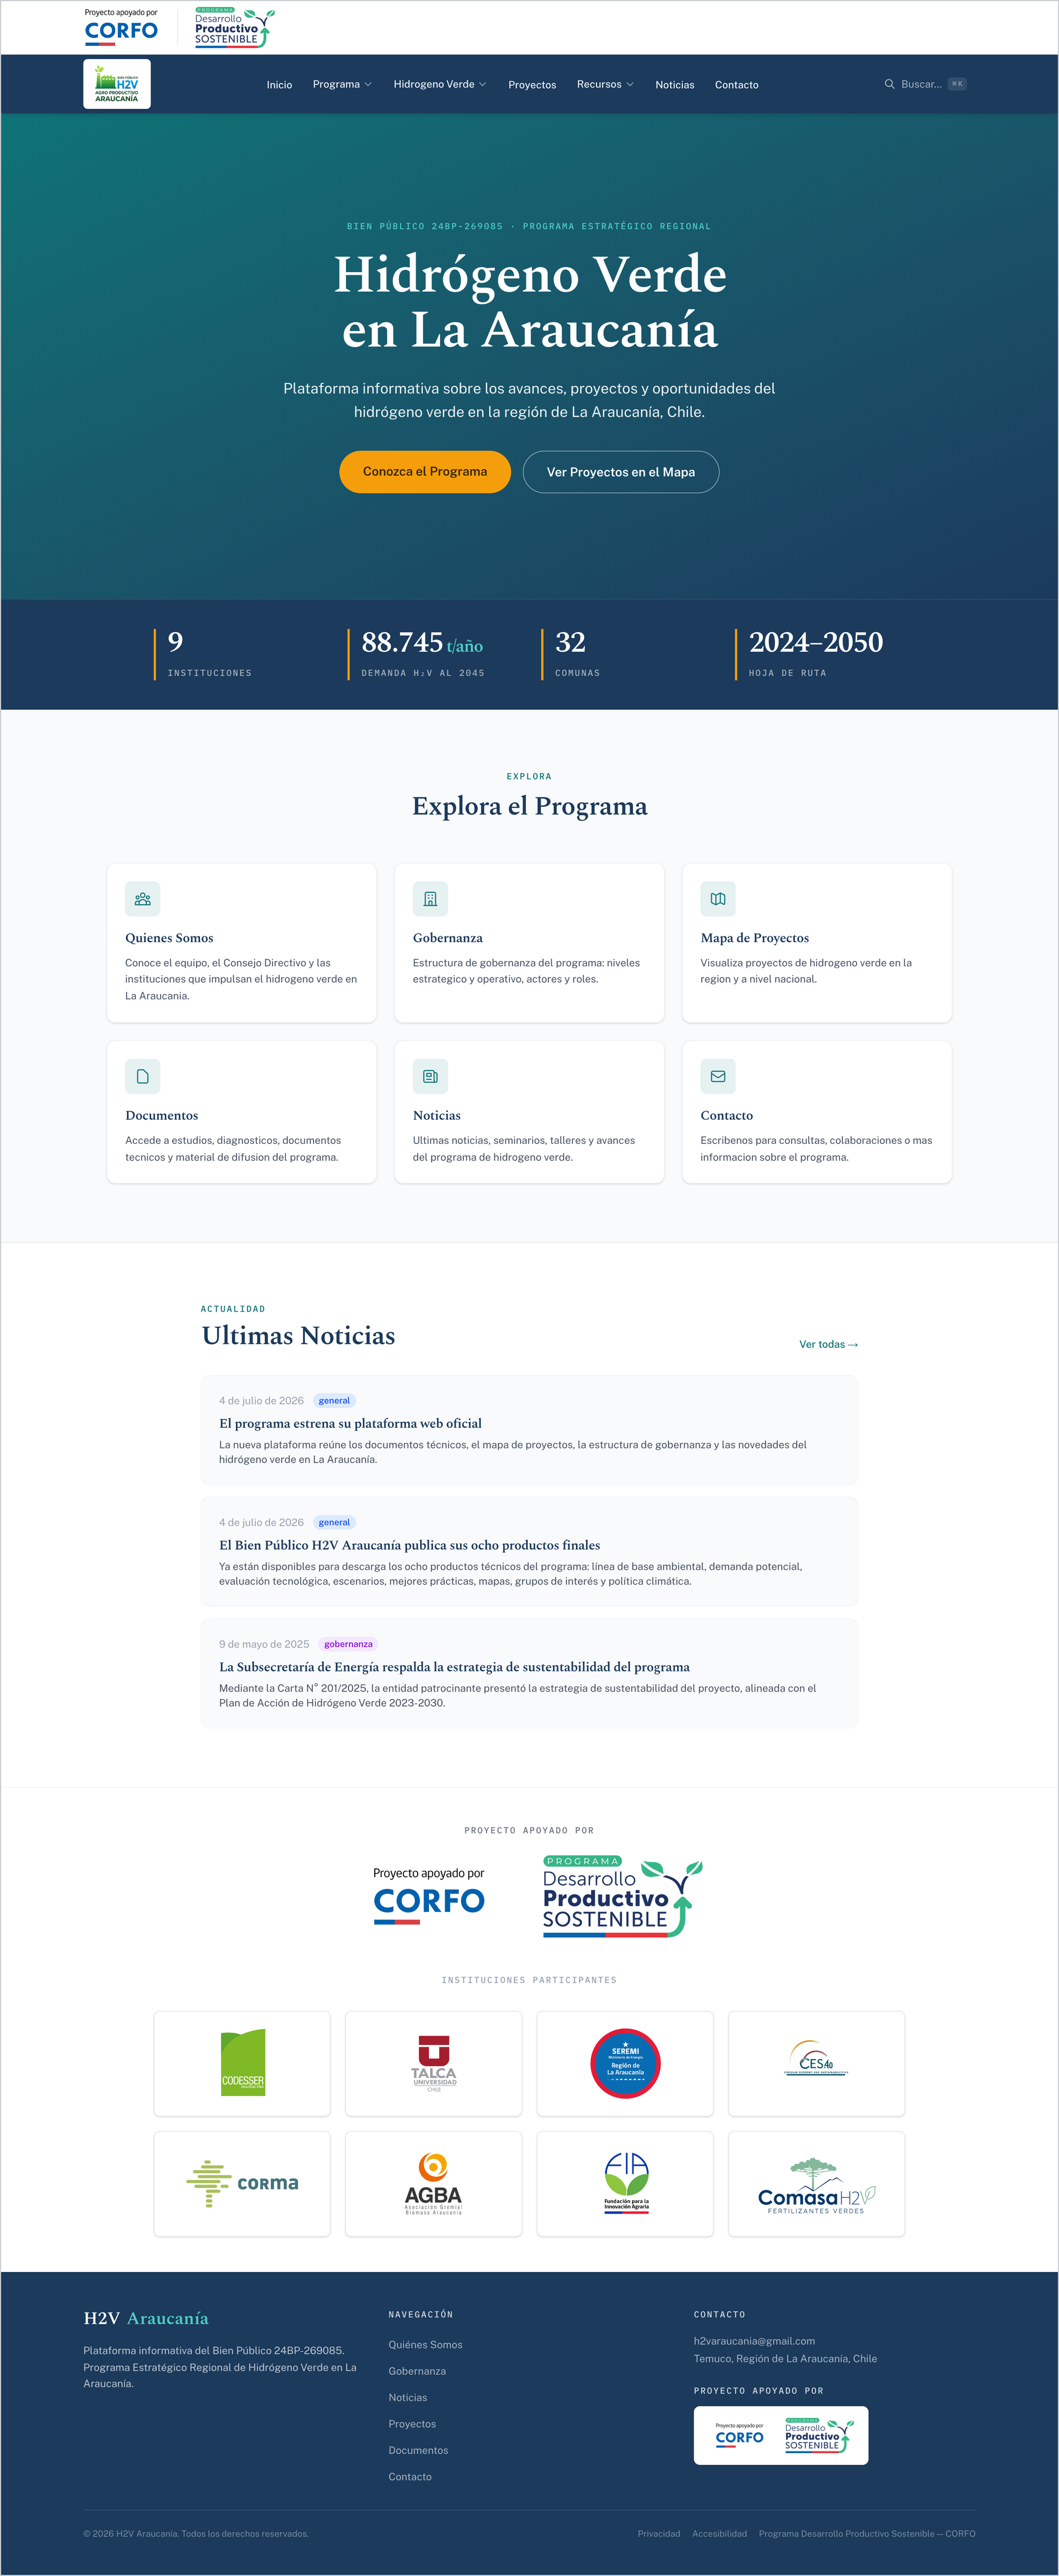
\includegraphics[width=\linewidth,height=0.74\textheight,keepaspectratio]{40-web-inicio.png}
\caption{Portada del sitio público tal como la ve cualquier visitante.}
\end{figure}
La siguiente tabla es el ''mapa'' que conviene tener a mano: qué se ve en el sitio y dónde se edita en el panel. Se explica en detalle en los capítulos siguientes.

\begin{longtable}{>{\raggedright\arraybackslash}p{0.542\textwidth}>{\raggedright\arraybackslash}p{0.388\textwidth}}
\rowcolor{h2vazul}\textbf{\color{white}Lo que se ve en el sitio público} & \textbf{\color{white}Dónde se edita en el panel} \\
\endfirsthead
\rowcolor{h2vazul}\textbf{\color{white}Lo que se ve en el sitio público} & \textbf{\color{white}Dónde se edita en el panel} \\
\endhead
Portada: línea superior, título, subtítulo, botones, cifras (KPIs), tarjetas ''Explora el Programa'', títulos de las secciones & Páginas $\rightarrow$ \textbf{Página de Inicio} \\ \midrule
\rowcolor{filaalt}Portada: las últimas noticias & Contenido $\rightarrow$ \textbf{Noticias} (aparecen solas las más recientes publicadas) \\ \midrule
Portada y pie de página: logos de instituciones participantes & Configuración $\rightarrow$ \textbf{Configuración General} $\rightarrow$ Logos institucionales \\ \midrule
\rowcolor{filaalt}Quiénes Somos: textos, descripción del Bien Público, instituciones, títulos de las secciones & Páginas $\rightarrow$ \textbf{Quiénes Somos} \\ \midrule
Quiénes Somos y Gobernanza: las personas del Comité Estratégico, del Comité Consultivo y de la Unidad de Coordinación & Contenido $\rightarrow$ \textbf{Miembros de Gobernanza} \\ \midrule
\rowcolor{filaalt}Gobernanza: niveles, funciones, diagrama, galería de fotos & Páginas $\rightarrow$ \textbf{Gobernanza} \\ \midrule
Hidrógeno Verde, Sectores Productivos, Capital Humano, Hoja de Ruta, Marco Regulatorio & Páginas $\rightarrow$ la página del mismo nombre \\ \midrule
\rowcolor{filaalt}Mapa de Proyectos: los puntos del mapa & Contenido $\rightarrow$ \textbf{Proyectos} \\ \midrule
Mapa de Proyectos: título y subtítulo de la página & Páginas $\rightarrow$ \textbf{Mapa de Proyectos} \\ \midrule
\rowcolor{filaalt}Recursos y Documentación & Contenido $\rightarrow$ \textbf{Documentos} \\ \midrule
Eventos & Contenido $\rightarrow$ \textbf{Eventos} \\ \midrule
\rowcolor{filaalt}Noticias & Contenido $\rightarrow$ \textbf{Noticias} \\ \midrule
Comunidad, Transparencia, Mediateca & Páginas $\rightarrow$ la página del mismo nombre \\ \midrule
\rowcolor{filaalt}Contacto: textos, formulario, correo y datos institucionales & Configuración $\rightarrow$ \textbf{Contacto} \\ \midrule
Contacto: los mensajes que escriben los visitantes en el formulario & Contenido $\rightarrow$ \textbf{Mensajes de contacto} (solo se leen; vea ''Leer los mensajes del formulario de Contacto'') \\ \midrule
\rowcolor{filaalt}Pie de página (títulos, derechos) y página ''no encontrada'' (404) & Configuración $\rightarrow$ \textbf{Configuración General} \\ \midrule
Política de Privacidad y Accesibilidad & Páginas $\rightarrow$ \textbf{Política de Privacidad} / \textbf{Accesibilidad} \\ \midrule
\rowcolor{filaalt}Nombre del sitio en la pestaña del navegador y en Google & Configuración $\rightarrow$ \textbf{Configuración General} \\ \bottomrule
\end{longtable}
\section{La regla de oro y sus excepciones}
La regla de oro del sitio es simple: \textbf{si usted lo ve en la web, se cambia en el panel}. Cada página tiene su formulario, cada texto tiene su campo, y cada campo tiene debajo una explicación breve de para qué sirve. Al guardar, el cambio se ve en el sitio en segundos: basta recargar la página del sitio público.

Hay unas pocas cosas que, a propósito, no se editan desde el panel:

\begin{itemize}
  \item \textbf{El diseño}: colores, tipografías, disposición de los elementos y animaciones.
  \item \textbf{El menú de navegación} (Inicio, Programa, Hidrógeno Verde, Proyectos, Recursos, Noticias, Contacto) y la estructura de las páginas.
  \item \textbf{El crédito obligatorio a CORFO} (''Proyecto apoyado por'' con el logo de CORFO y del programa Desarrollo Productivo Sostenible), que exige el Manual de Comunicaciones de CORFO y por eso está fijo, para que no pueda borrarse por error.
  \item \textbf{La dirección de correo a la que llegan los avisos del formulario de contacto} (se configura en el servidor, no en el panel; vea el Anexo D). Los mensajes mismos sí se leen en el panel, en Contenido $\rightarrow$ Mensajes de contacto.
\end{itemize}
Para cualquiera de esas cosas hay que pedir el cambio al soporte técnico (vea el Anexo D, ''Ficha técnica de la plataforma'').

\section{Qué necesita para trabajar}
\begin{itemize}
  \item Un computador con un navegador actualizado (Chrome, Edge, Firefox o Safari). El panel también funciona en tablet, pero es más cómodo en pantalla grande.
  \item Una \textbf{cuenta} en el panel: un correo electrónico y una contraseña. La crea una persona con rol Administrador (vea el capítulo ''Usuarios, roles y seguridad'').
  \item Conexión a internet.
\end{itemize}
\chapter{Entrar y salir del panel}
\section{Entrar al panel}
\begin{enumerate}
  \item Abra el navegador y escriba la dirección del sitio seguida de \url{/admin}. Por ejemplo: \url{https://h2v-araucania.vercel.app/admin}.
  \item Escriba su \textbf{Correo electrónico} (1) y su \textbf{Contraseña} (2).
  \item Haga clic en \textbf{Iniciar sesión} (3).
\end{enumerate}
\begin{figure}[H]\centering
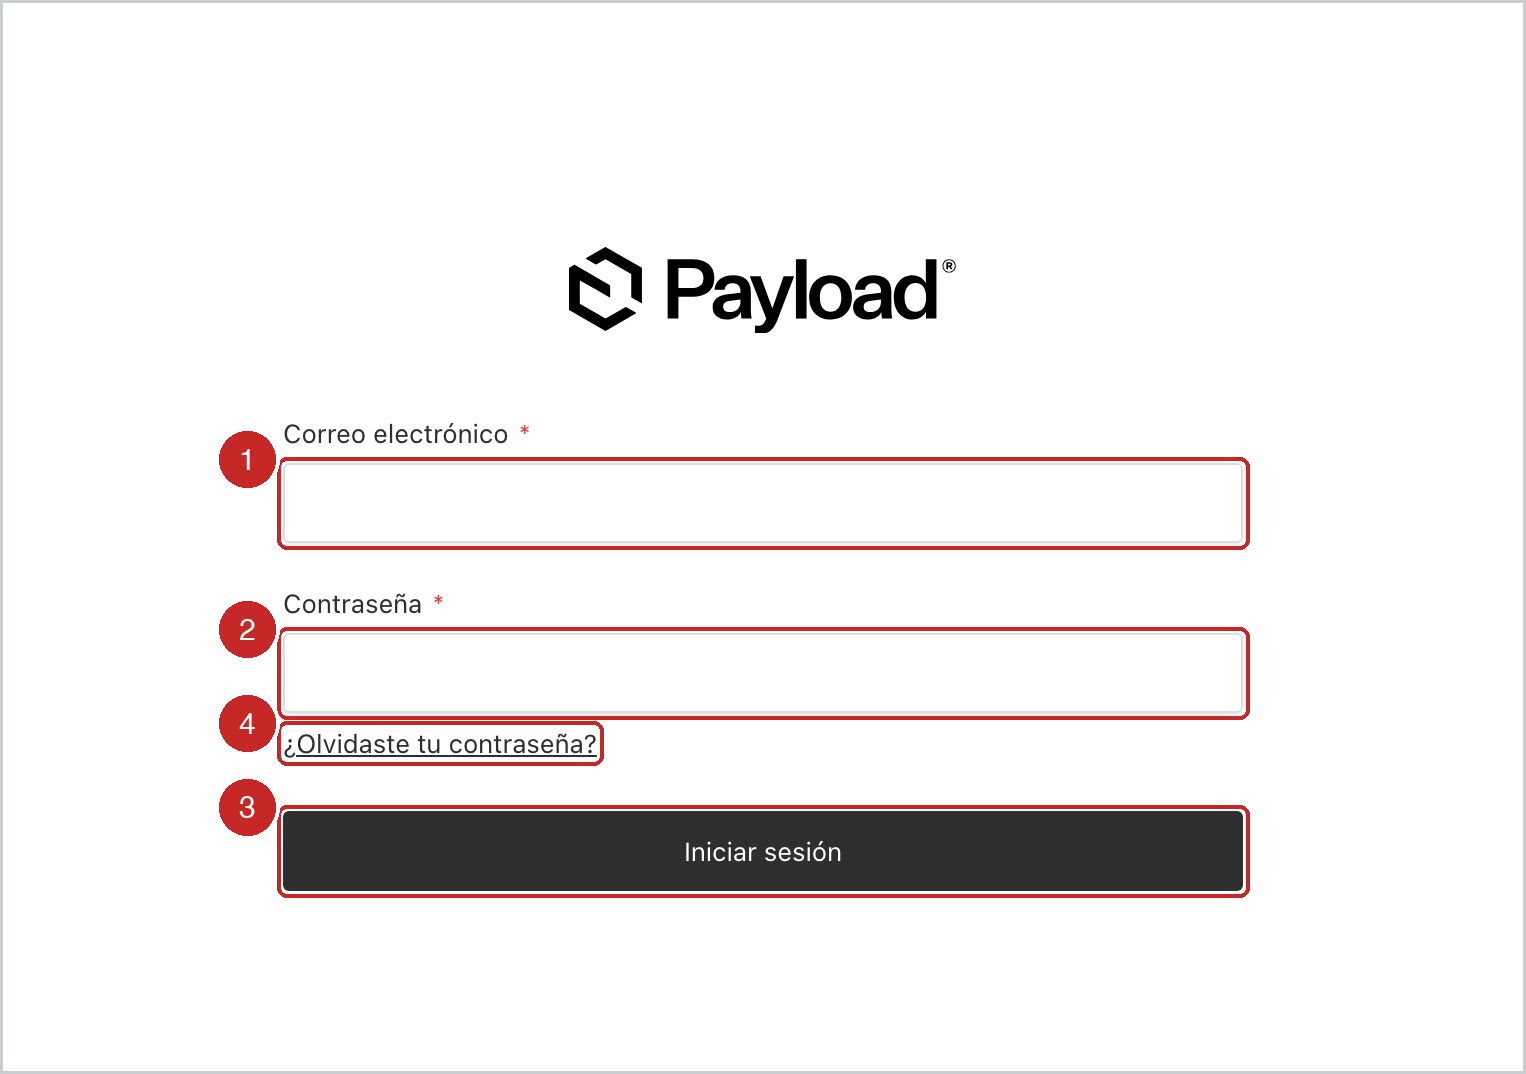
\includegraphics[width=\linewidth,keepaspectratio]{01-login.png}
\caption{Pantalla de entrada al panel: correo (1), contraseña (2), botón de entrar (3) y enlace para recuperar la contraseña (4).}
\end{figure}
\begin{recuadro}{cResultado}{bResultado}\textbf{\color{bResultado}Resultado:} se abre el ''Panel de Control'', con los grupos Cuentas y acceso, Sistema, Contenido, Configuración, Páginas y Ayuda.\end{recuadro}
\begin{recuadro}{cConsejo}{bConsejo}\textbf{\color{bConsejo}Consejo:} guarde la dirección del panel en los favoritos del navegador. El navegador también puede recordar la contraseña; úselo solo en un computador institucional y personal, nunca en uno compartido.\end{recuadro}
\section{Olvidé mi contraseña}
Pida a un Administrador que le deje escribir una contraseña nueva, \textbf{con usted presente}:

\begin{enumerate}
  \item El Administrador abre \textbf{Usuarios} (grupo Cuentas y acceso), hace clic en su correo y pulsa \textbf{Cambiar contraseña}.
  \item Usted escribe la contraseña nueva en \textbf{Nueva Contraseña} y otra vez en \textbf{Confirmar Contraseña}. El Administrador no mira.
  \item El Administrador pulsa \textbf{Guardar}. Usted ya puede entrar con la contraseña nueva.
\end{enumerate}
\begin{recuadro}{cAtencion}{bAtencion}\textbf{\color{bAtencion}Atención:} la pantalla de entrada tiene un enlace \textbf{¿Olvidaste tu contraseña?} (4 en la figura anterior), que envía un correo para crear una contraseña nueva. Mientras el sitio no tenga dominio propio, \textbf{ese correo no llega a los correos institucionales}: solo llega a la dirección con que se creó el servicio de correo del sitio. Cuando el sitio tenga su dominio (Anexo D), cada persona podrá usarlo sola, así:\end{recuadro}
\begin{enumerate}
  \item En la pantalla de entrada, haga clic en \textbf{¿Olvidaste tu contraseña?}.
  \item Escriba el correo electrónico de su cuenta (1) y haga clic en el botón de enviar (2).
  \item Revise su bandeja de entrada (y la carpeta de correo no deseado). Recibirá un mensaje con un enlace para crear una contraseña nueva. El enlace dura un tiempo limitado; si expiró, repita el procedimiento.
\end{enumerate}
\begin{figure}[H]\centering
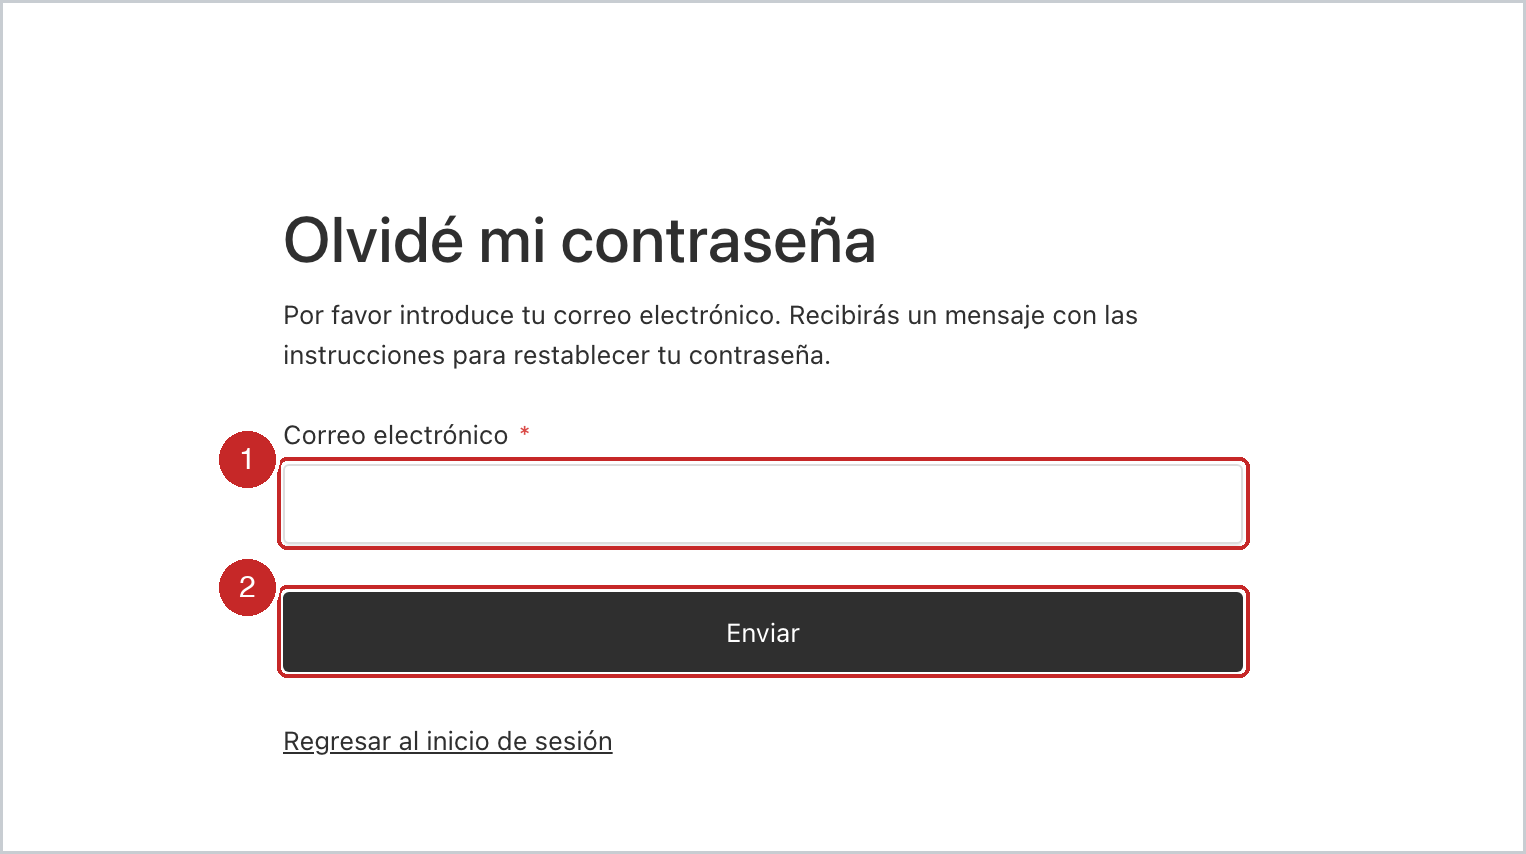
\includegraphics[width=\linewidth,keepaspectratio]{02-olvide-clave.png}
\caption{Recuperación de contraseña: correo (1) y botón de enviar (2).}
\end{figure}
\section{Me bloqueé: ''demasiados intentos''}
Por seguridad, después de \textbf{5 intentos fallidos} de contraseña la cuenta se bloquea durante \textbf{10 minutos}. No es una falla: espere 10 minutos y vuelva a intentar. Si no recuerda la contraseña, vea ''Olvidé mi contraseña''. Un Administrador también puede desbloquear la cuenta de inmediato desde Usuarios (botón \textbf{Forzar Desbloqueo} en la ficha del usuario).

\section{Cambiar mi contraseña y cerrar sesión}
\begin{enumerate}
  \item Haga clic en el círculo de la esquina superior derecha (su cuenta) y entre a su perfil, o vaya directamente a la dirección del sitio seguida de \url{/admin/account}.
  \item Haga clic en \textbf{Cambiar contraseña} (1), escriba la nueva contraseña dos veces y pulse \textbf{Guardar}.
  \item Para salir, en el mismo menú de su cuenta elija \textbf{Cerrar sesión} (o visite \url{/admin/logout}).
\end{enumerate}
\begin{figure}[H]\centering
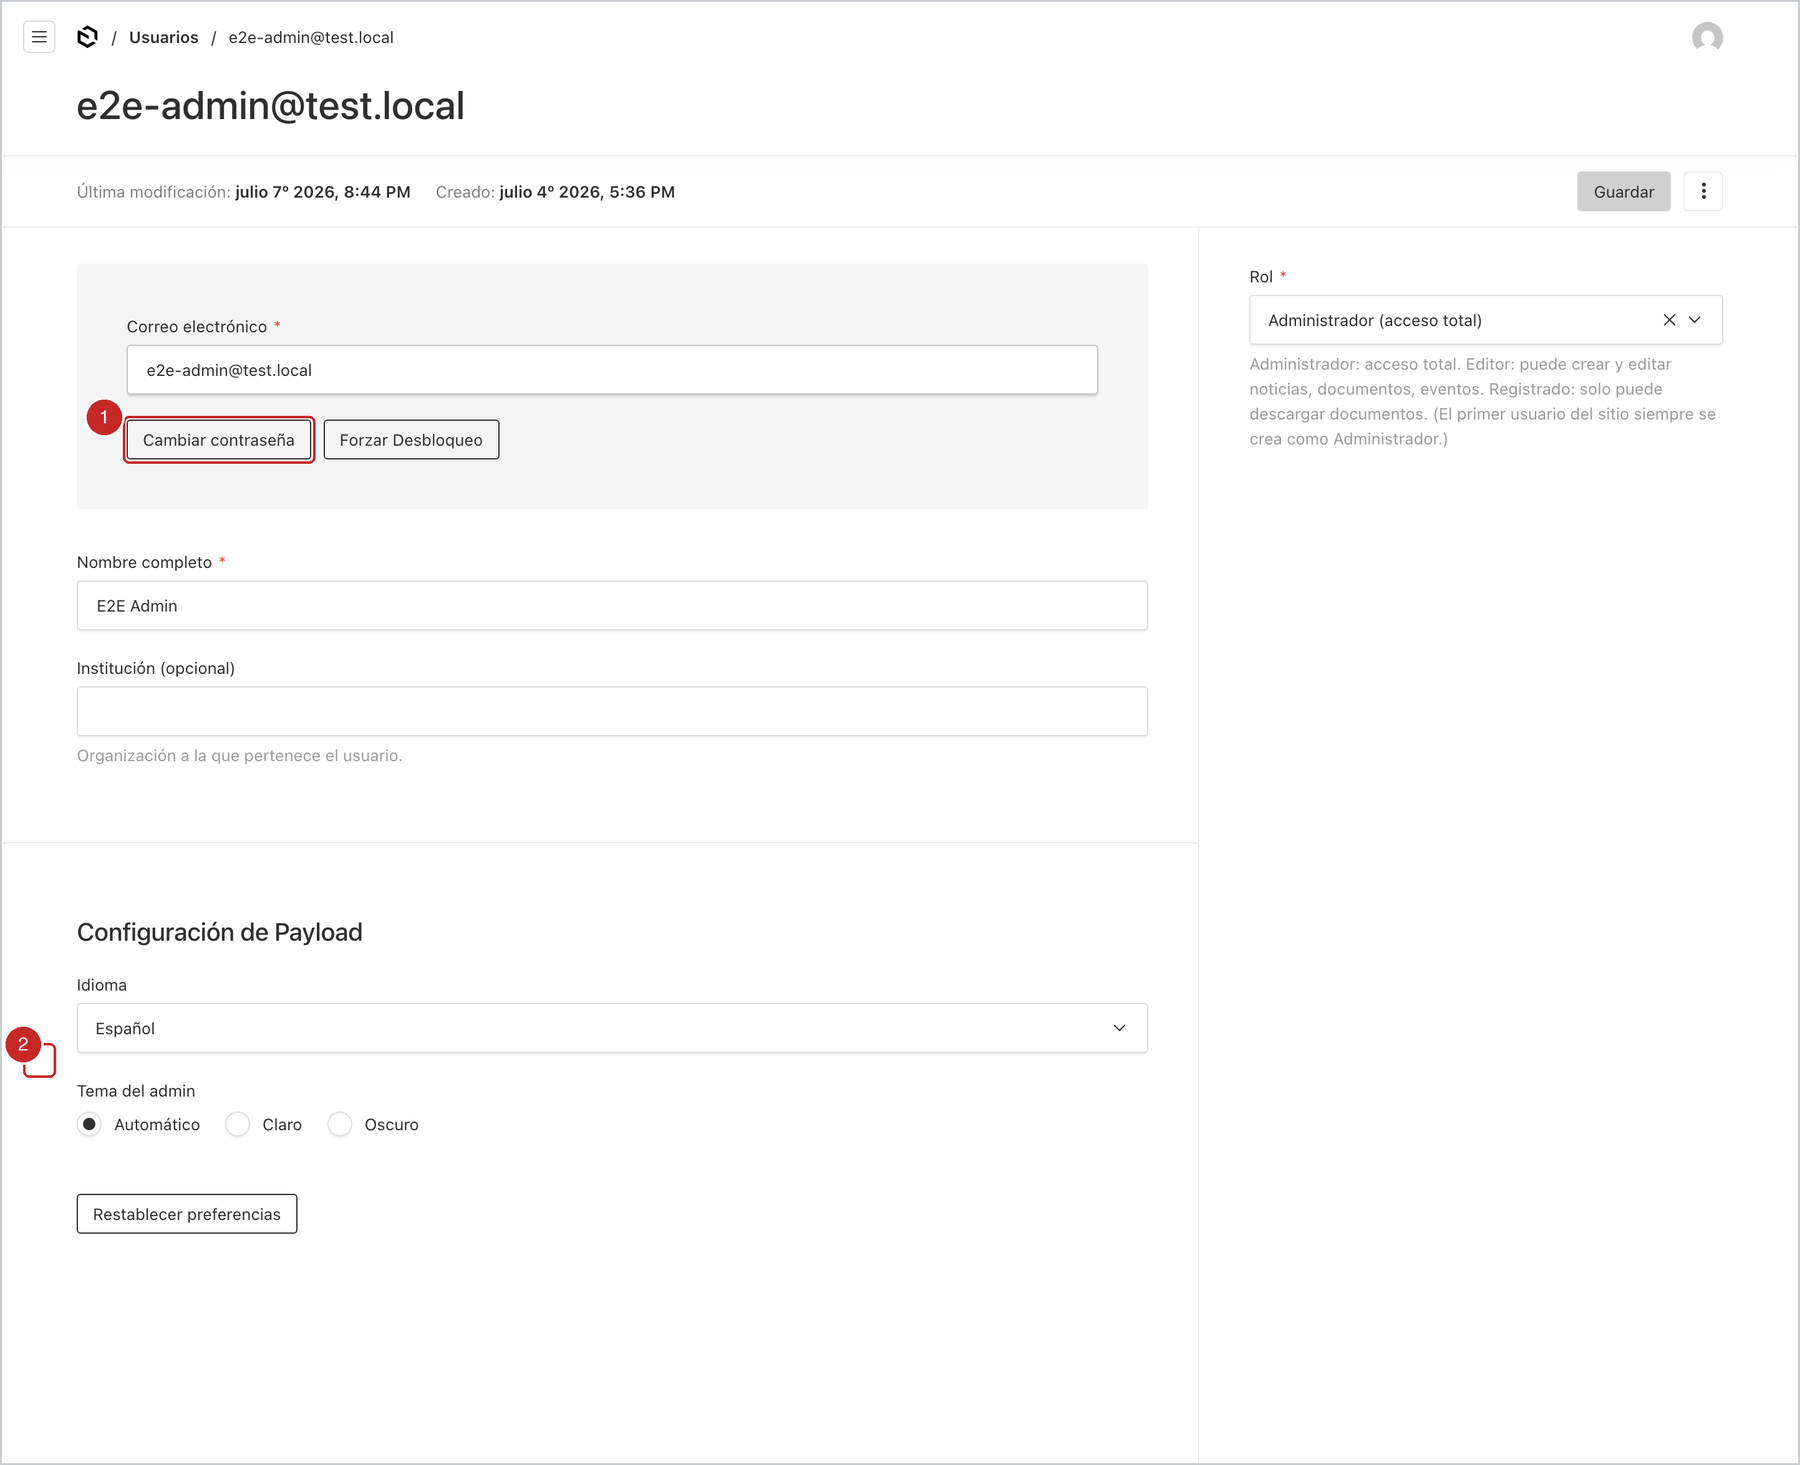
\includegraphics[width=\linewidth,keepaspectratio]{32-mi-cuenta.png}
\caption{Página ''Mi cuenta'': botón Cambiar contraseña (1). En esta página también puede elegir el idioma del panel y el tema claro u oscuro.}
\end{figure}
\begin{figure}[H]\centering
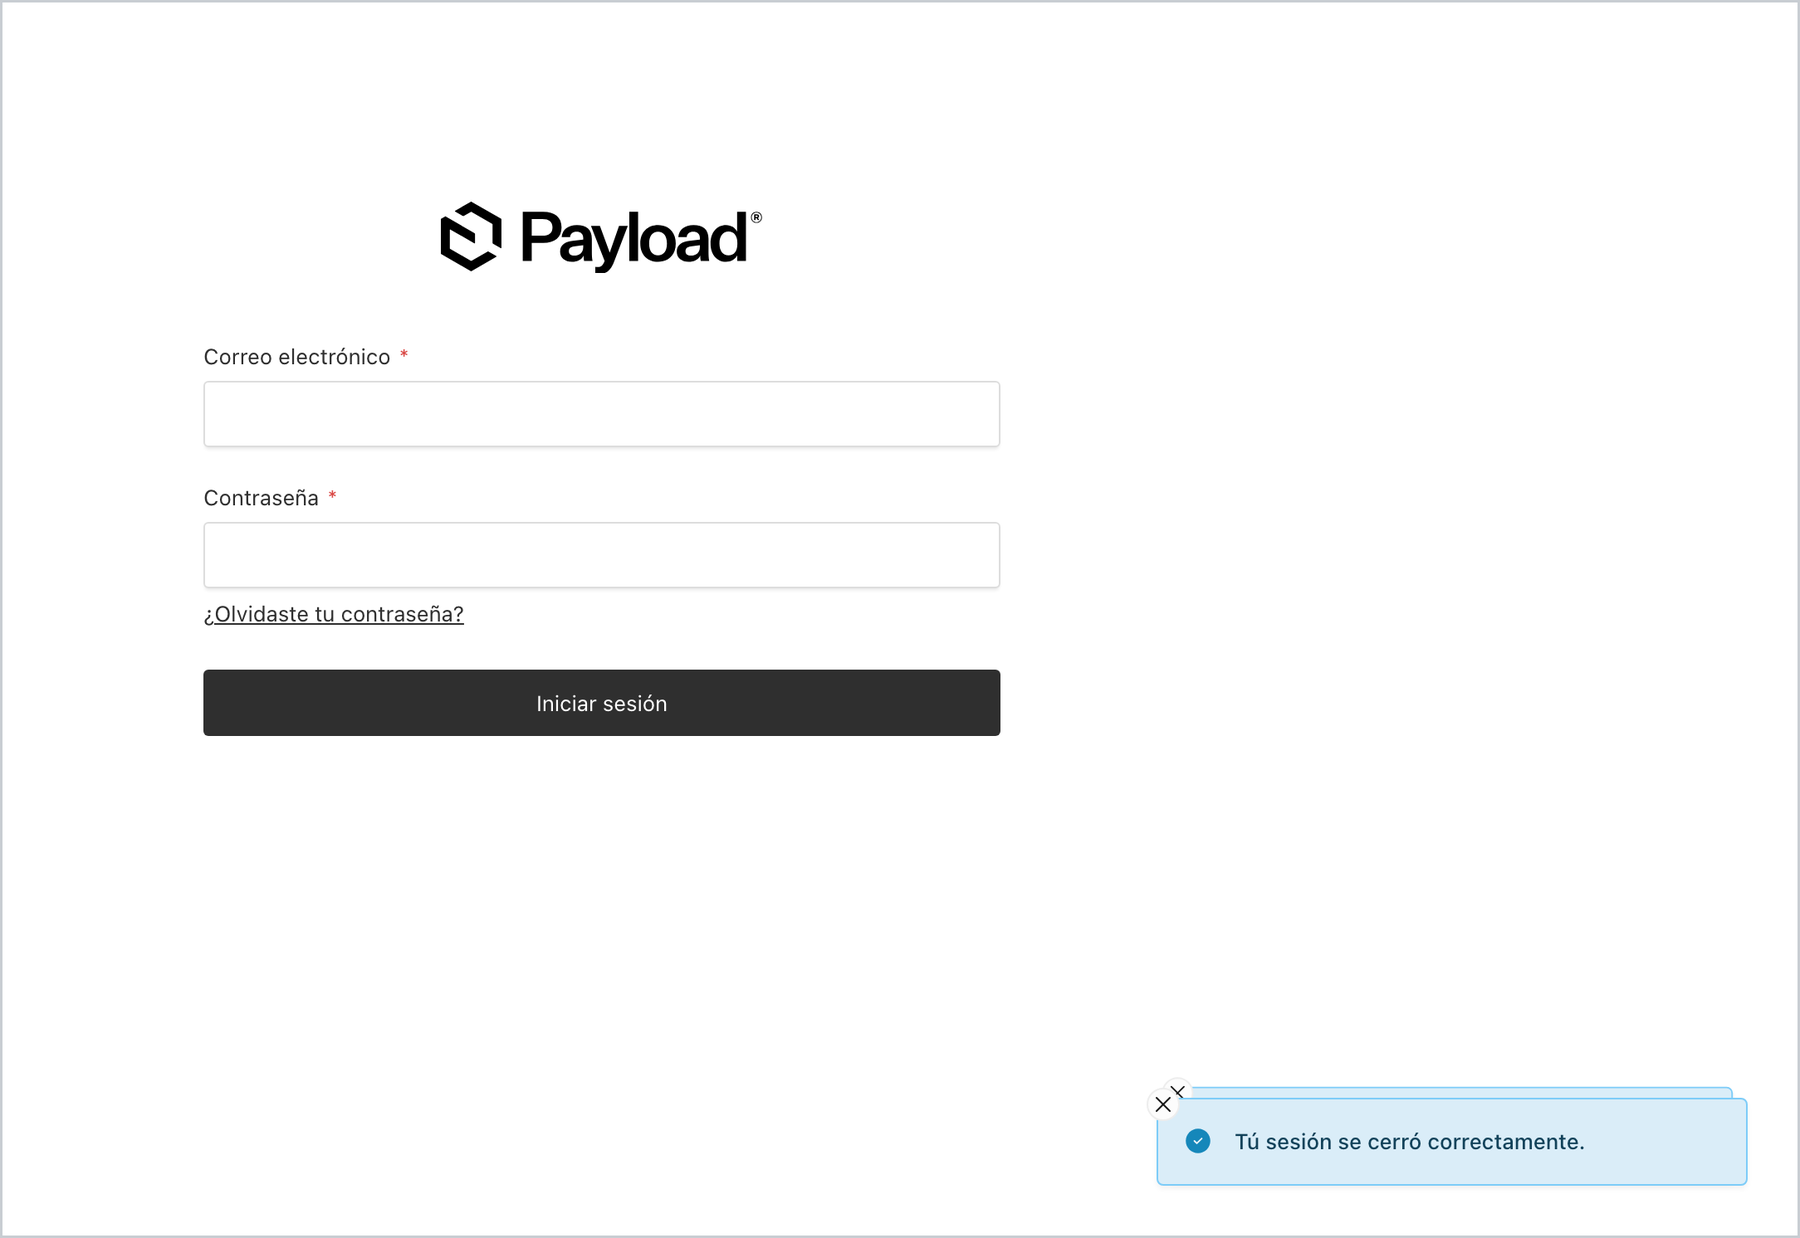
\includegraphics[width=\linewidth,keepaspectratio]{33-salir.png}
\caption{Confirmación de que la sesión se cerró correctamente.}
\end{figure}
\begin{recuadro}{cSeguridad}{bSeguridad}\textbf{\color{bSeguridad}Seguridad:} cierre sesión siempre que use un computador que no sea el suyo. Use contraseñas largas (12 caracteres o más), distintas a las de otros servicios, y no las comparta por correo ni por WhatsApp.\end{recuadro}
\chapter{Conocer el panel}
\section{El Panel de Control}
Al entrar se ve el \textbf{Panel de Control}: una página con tarjetas agrupadas. Cada tarjeta lleva a una lista (Noticias, Documentos...) o al formulario de una página del sitio (Página de Inicio, Quiénes Somos...). El botón con el símbolo ''+'' en una tarjeta crea un elemento nuevo directamente.

\begin{figure}[H]\centering
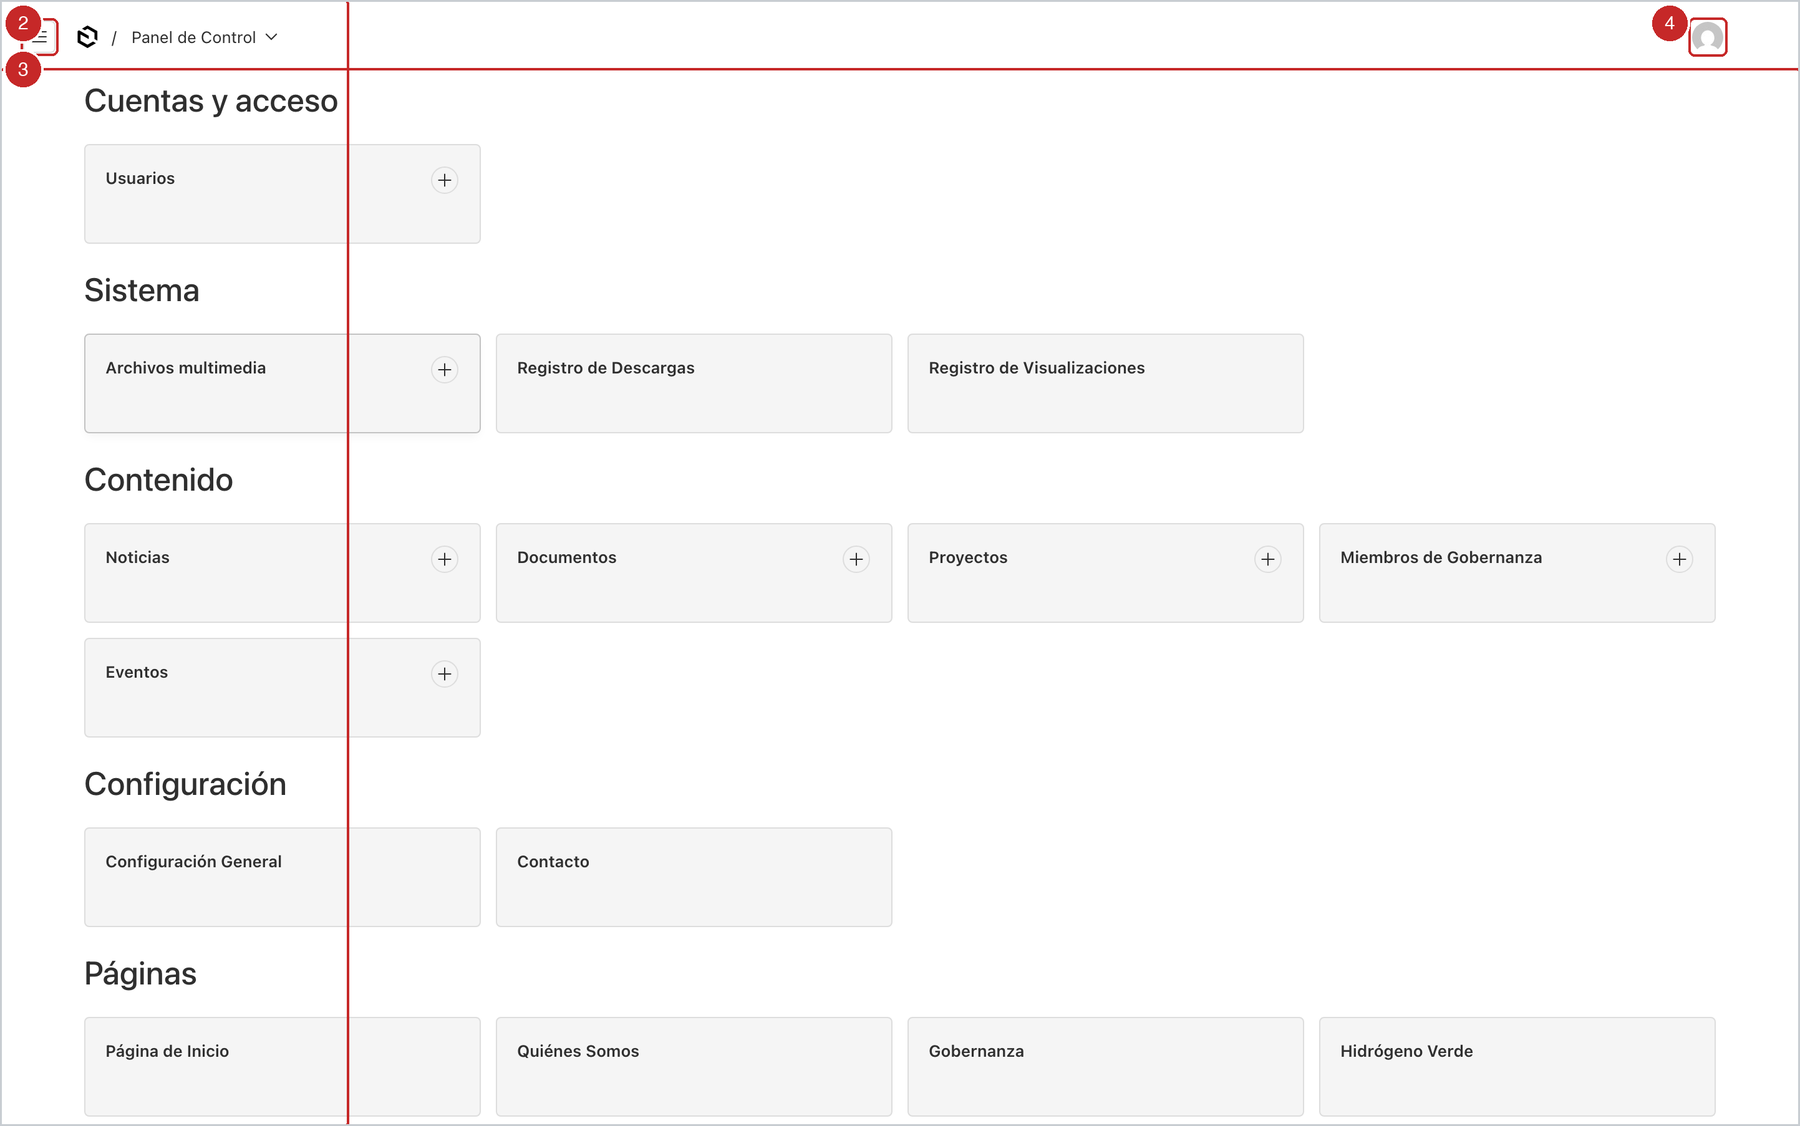
\includegraphics[width=\linewidth,keepaspectratio]{03b-panel-menu-abierto.png}
\caption{Panel de Control con los grupos de tarjetas. Arriba a la izquierda, el botón de menú (1) abre el menú lateral; arriba a la derecha, el círculo de su cuenta (4).}
\end{figure}
Los grupos son:

\begin{longtable}{>{\raggedright\arraybackslash}p{0.178\textwidth}>{\raggedright\arraybackslash}p{0.550\textwidth}>{\raggedright\arraybackslash}p{0.202\textwidth}}
\rowcolor{h2vazul}\textbf{\color{white}Grupo} & \textbf{\color{white}Qué contiene} & \textbf{\color{white}Quién lo ve} \\
\endfirsthead
\rowcolor{h2vazul}\textbf{\color{white}Grupo} & \textbf{\color{white}Qué contiene} & \textbf{\color{white}Quién lo ve} \\
\endhead
\textbf{Contenido} & Noticias, Documentos, Proyectos, Miembros de Gobernanza, Eventos. Lo que se publica con frecuencia. & Administradores y editores \\ \midrule
\rowcolor{filaalt}\textbf{Páginas} & Un formulario por cada página del sitio: Página de Inicio, Quiénes Somos, Gobernanza, Hidrógeno Verde, Sectores Productivos, Hoja de Ruta, Comunidad, Capital Humano, Marco Regulatorio, Transparencia, Mediateca, Mapa de Proyectos, Política de Privacidad, Accesibilidad. & Administradores y editores \\ \midrule
\textbf{Configuración} & Configuración General (nombre del sitio, pie de página, logos) y Contacto (datos institucionales y formulario). & Solo administradores \\ \midrule
\rowcolor{filaalt}\textbf{Sistema} & Archivos multimedia (todas las imágenes y PDF subidos), Registro de Descargas y Registro de Visualizaciones (estadísticas automáticas, solo lectura). & Administradores y editores \\ \midrule
\textbf{Cuentas y acceso} & Usuarios. & Solo administradores \\ \midrule
\rowcolor{filaalt}\textbf{Ayuda} & Guía de uso: un resumen de este manual dentro del propio panel. & Todos \\ \bottomrule
\end{longtable}
\section{El menú lateral}
El menú lateral se abre y se cierra con el botón de tres líneas de la esquina superior izquierda. Tiene los mismos grupos que el Panel de Control; cada grupo se puede plegar o desplegar haciendo clic en su nombre. Es la forma más rápida de moverse por el panel.

\begin{figure}[H]\centering
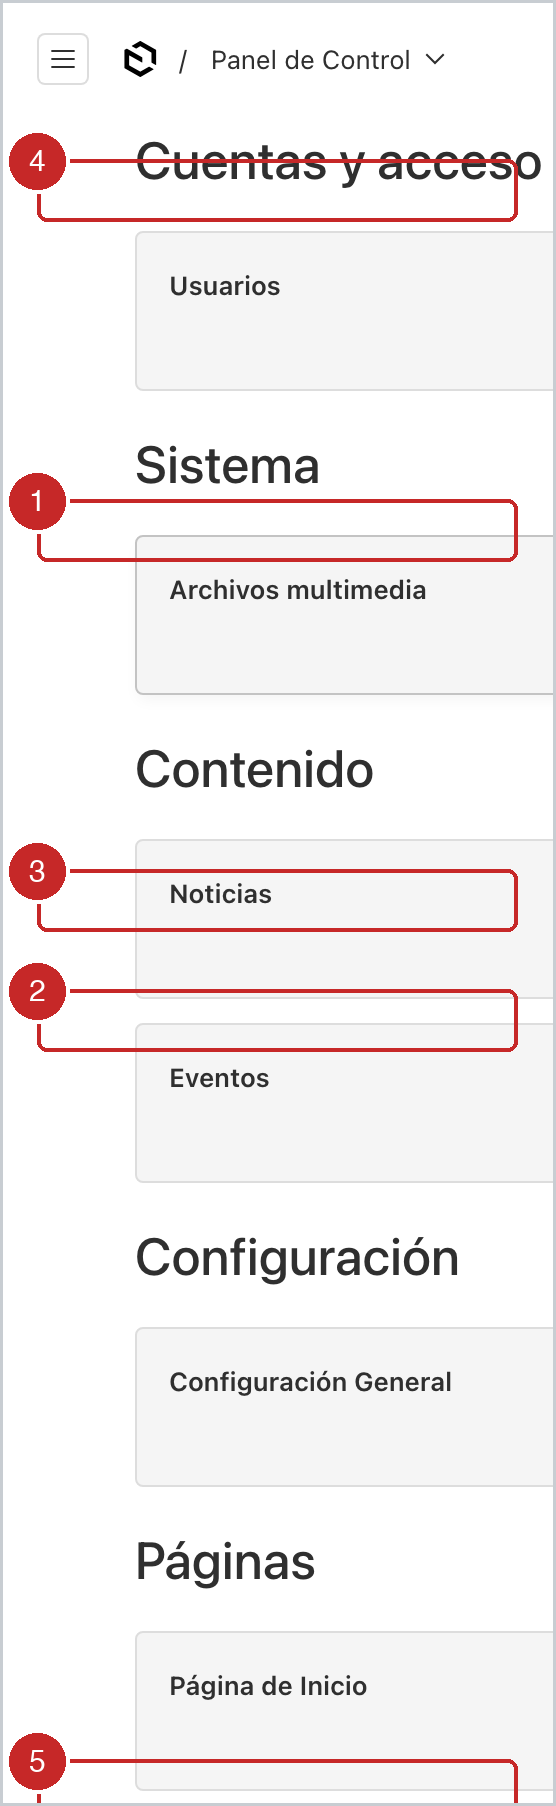
\includegraphics[width=\linewidth,height=0.74\textheight,keepaspectratio]{04-menu-lateral.png}
\caption{Menú lateral desplegado. Señalados: Noticias (1), Página de Inicio (2), Contacto (3), Usuarios (4) y la Guía de uso (5).}
\end{figure}
\section{Dos tipos de cosas: listas y páginas}
En el panel hay dos tipos de cosas, y conviene distinguirlas desde el principio:

\begin{itemize}
  \item \textbf{Listas} (en el panel se llaman ''colecciones''): Noticias, Documentos, Proyectos, Miembros de Gobernanza, Eventos, Archivos multimedia, Usuarios. Son conjuntos de elementos: usted crea uno nuevo, lo edita o lo elimina. Al entrar se ve una tabla con todos los elementos y el botón \textbf{Crear nuevo}.
  \item \textbf{Páginas} (en el panel se llaman ''globales''): Página de Inicio, Quiénes Somos, Gobernanza, Contacto, Configuración General, etc. Cada una es un único formulario con los textos de esa página del sitio. No se crean ni se borran: solo se editan y se guardan.
\end{itemize}
\begin{figure}[H]\centering
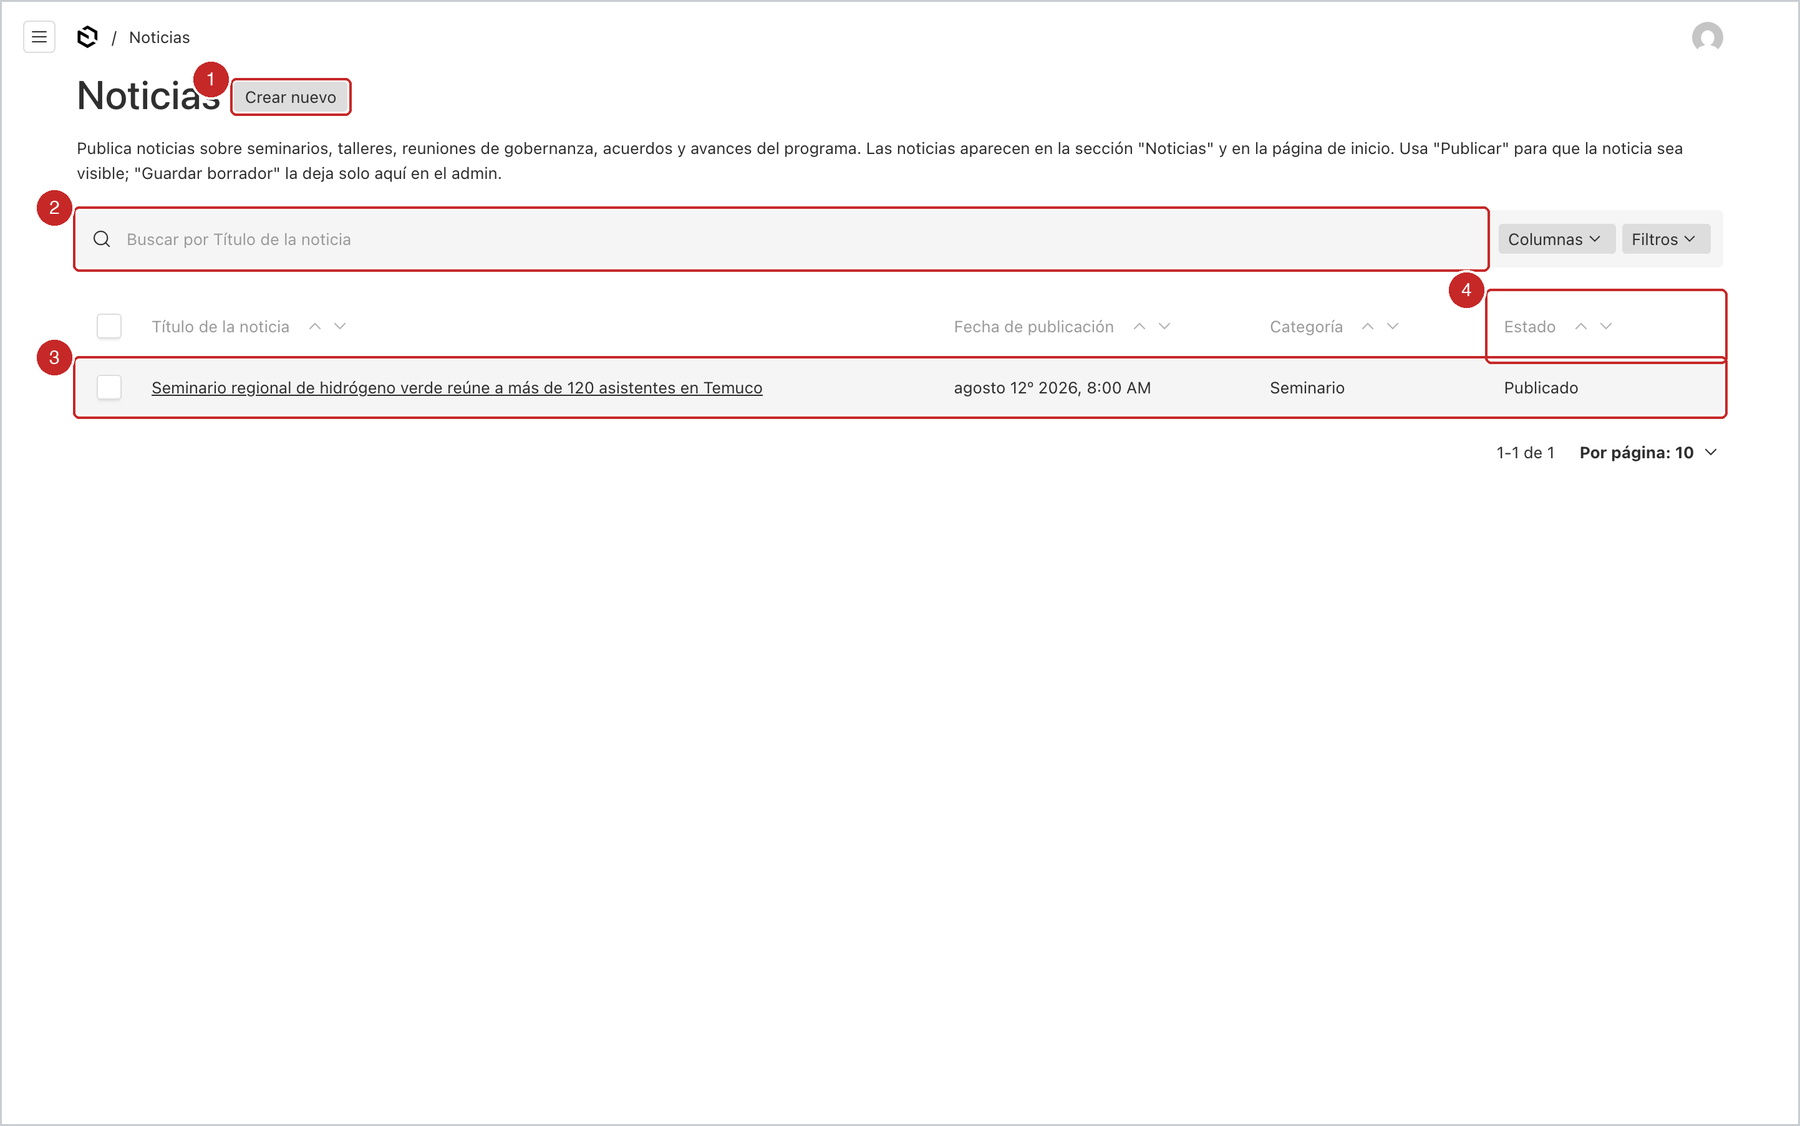
\includegraphics[width=\linewidth,keepaspectratio]{05-noticias-lista.png}
\caption{Lista de Noticias: botón Crear nuevo (1), buscador (2), filas de la tabla (3) y columna de estado (4). Al hacer clic en una fila se abre la noticia para editarla.}
\end{figure}
\section{Anatomía de un formulario}
Todos los formularios del panel se parecen. Tomemos como ejemplo el formulario de una noticia nueva:

\begin{figure}[H]\centering
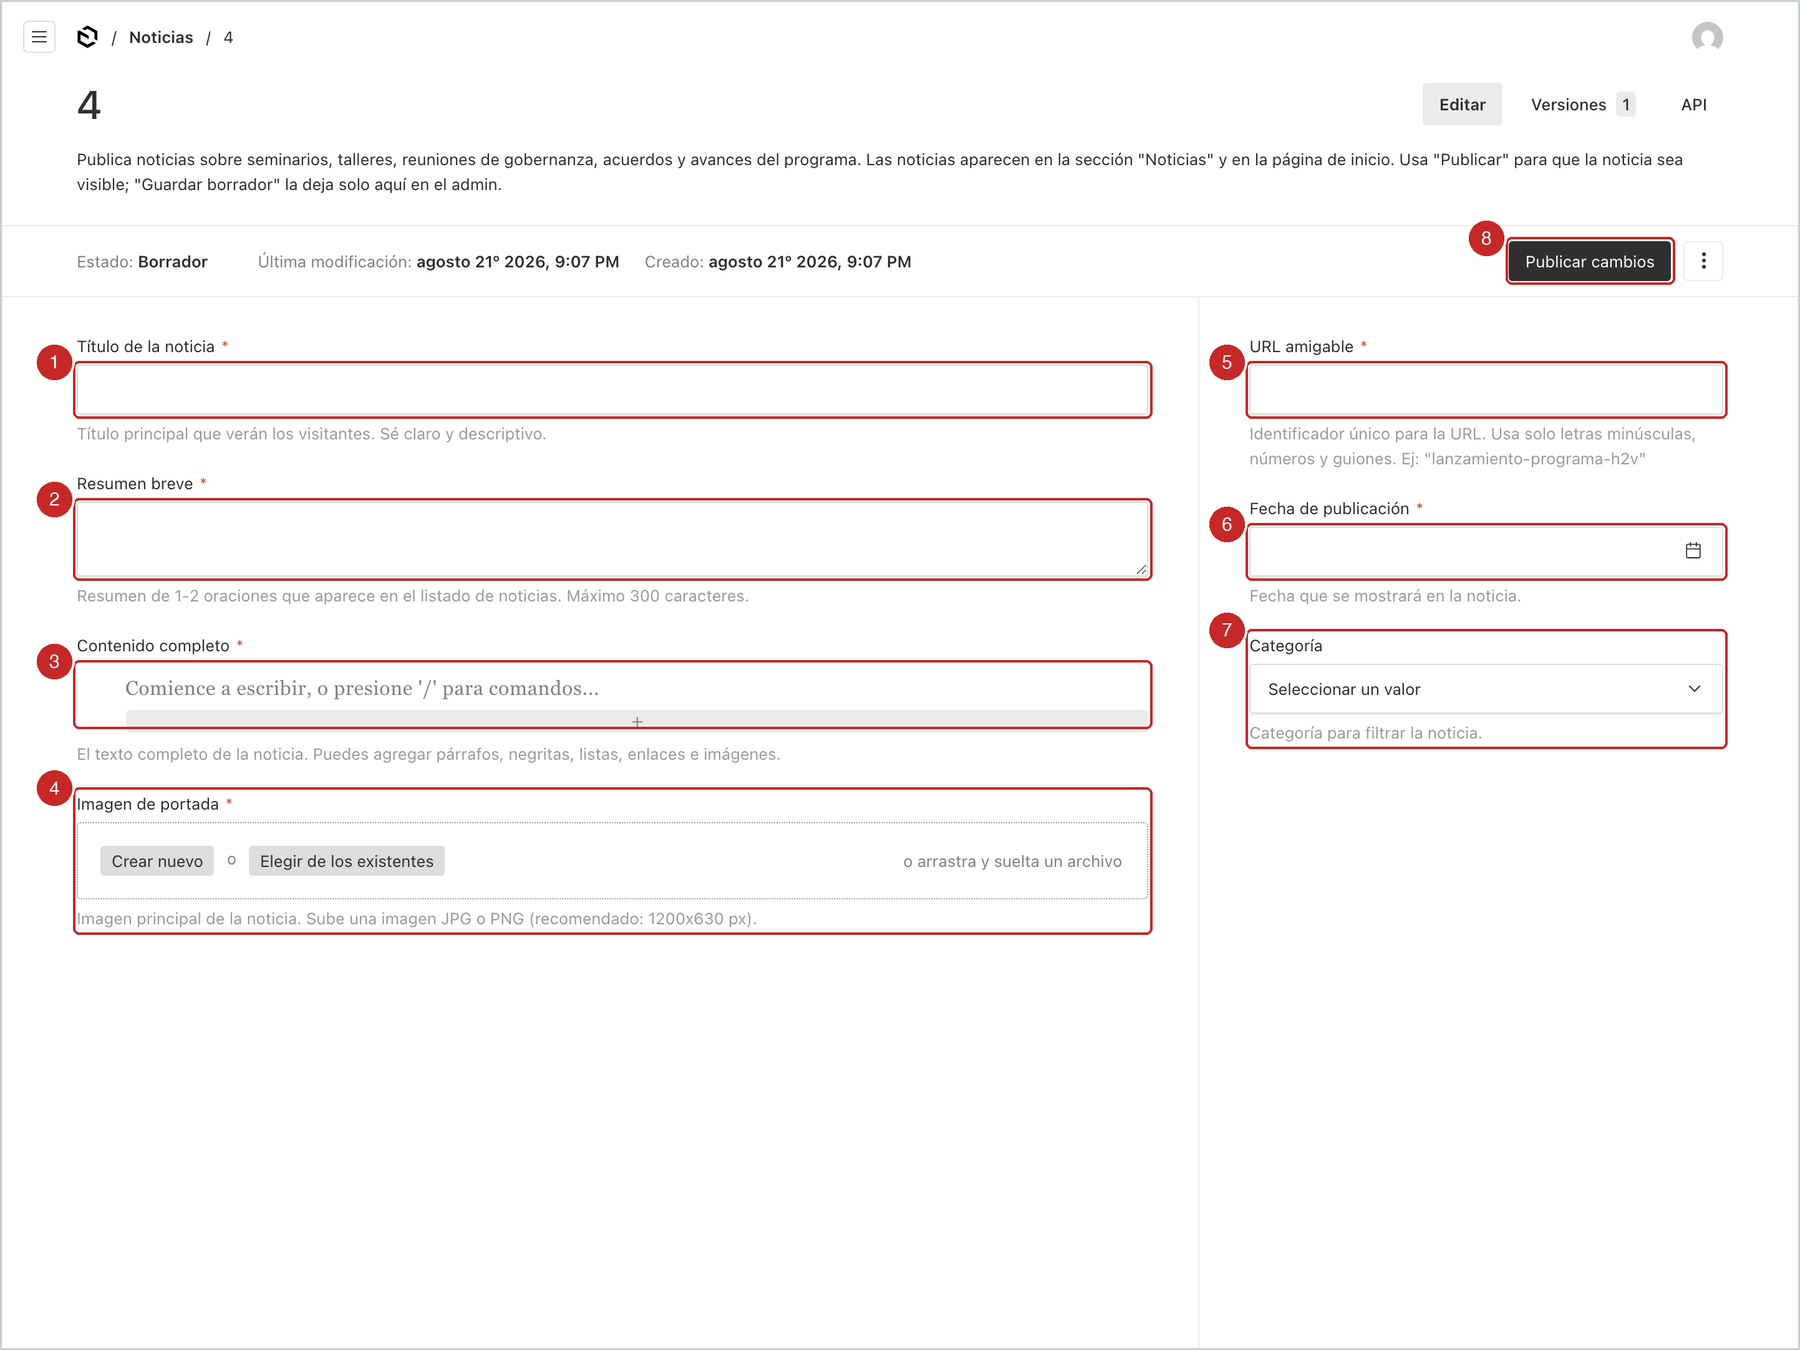
\includegraphics[width=\linewidth,keepaspectratio]{06-noticia-crear.png}
\caption{Formulario de una noticia nueva. Campos principales (1 a 4), barra lateral (5 a 7) y botón Publicar cambios (8).}
\end{figure}
\begin{itemize}
  \item \textbf{Título del formulario y descripción}: arriba, el nombre de lo que está editando y una frase que explica para qué sirve.
  \item \textbf{Barra de estado}: muestra si el elemento está en \textbf{Borrador} o \textbf{Publicado}, cuándo se modificó por última vez, y a la derecha el botón principal (\textbf{Publicar cambios} o \textbf{Guardar}, según el caso) y un botón de tres puntos con acciones adicionales (Duplicar, Eliminar).
  \item \textbf{Campos principales} (columna izquierda): los textos, el contenido, las imágenes.
  \item \textbf{Barra lateral} (columna derecha): los datos de clasificación, como la URL amigable, la fecha o la categoría.
  \item \textbf{Asterisco rojo} junto al nombre de un campo: el campo es obligatorio. Si falta, el panel no deja guardar y marca el campo en rojo.
  \item \textbf{Texto gris bajo cada campo}: la explicación de qué escribir. Léala siempre antes de llenar el campo; ahí están los ejemplos y los límites de largo.
  \item \textbf{Pestañas Editar / Versiones / API} (arriba a la derecha, en las noticias y eventos): ''Versiones'' guarda el historial de cada guardado y permite volver atrás.
\end{itemize}
\section{Borrador, publicado y versiones}
Las \textbf{Noticias} y los \textbf{Eventos} tienen dos estados:

\begin{itemize}
  \item \textbf{Borrador}: está guardado en el panel pero \textbf{no se ve en el sitio público}. Sirve para preparar una noticia con calma o terminarla otro día.
  \item \textbf{Publicado}: se ve en el sitio público.
\end{itemize}
Mientras usted escribe una noticia o un evento, el panel \textbf{guarda el borrador automáticamente} cada pocos segundos (por eso no hay un botón ''Guardar borrador'': no hace falta). Para que el contenido se vea en el sitio, debe pulsar el botón \textbf{Publicar cambios}. Si después modifica una noticia ya publicada, los cambios quedan como borrador hasta que vuelva a pulsar \textbf{Publicar cambios}; mientras tanto, el sitio sigue mostrando la última versión publicada.

\begin{figure}[H]\centering
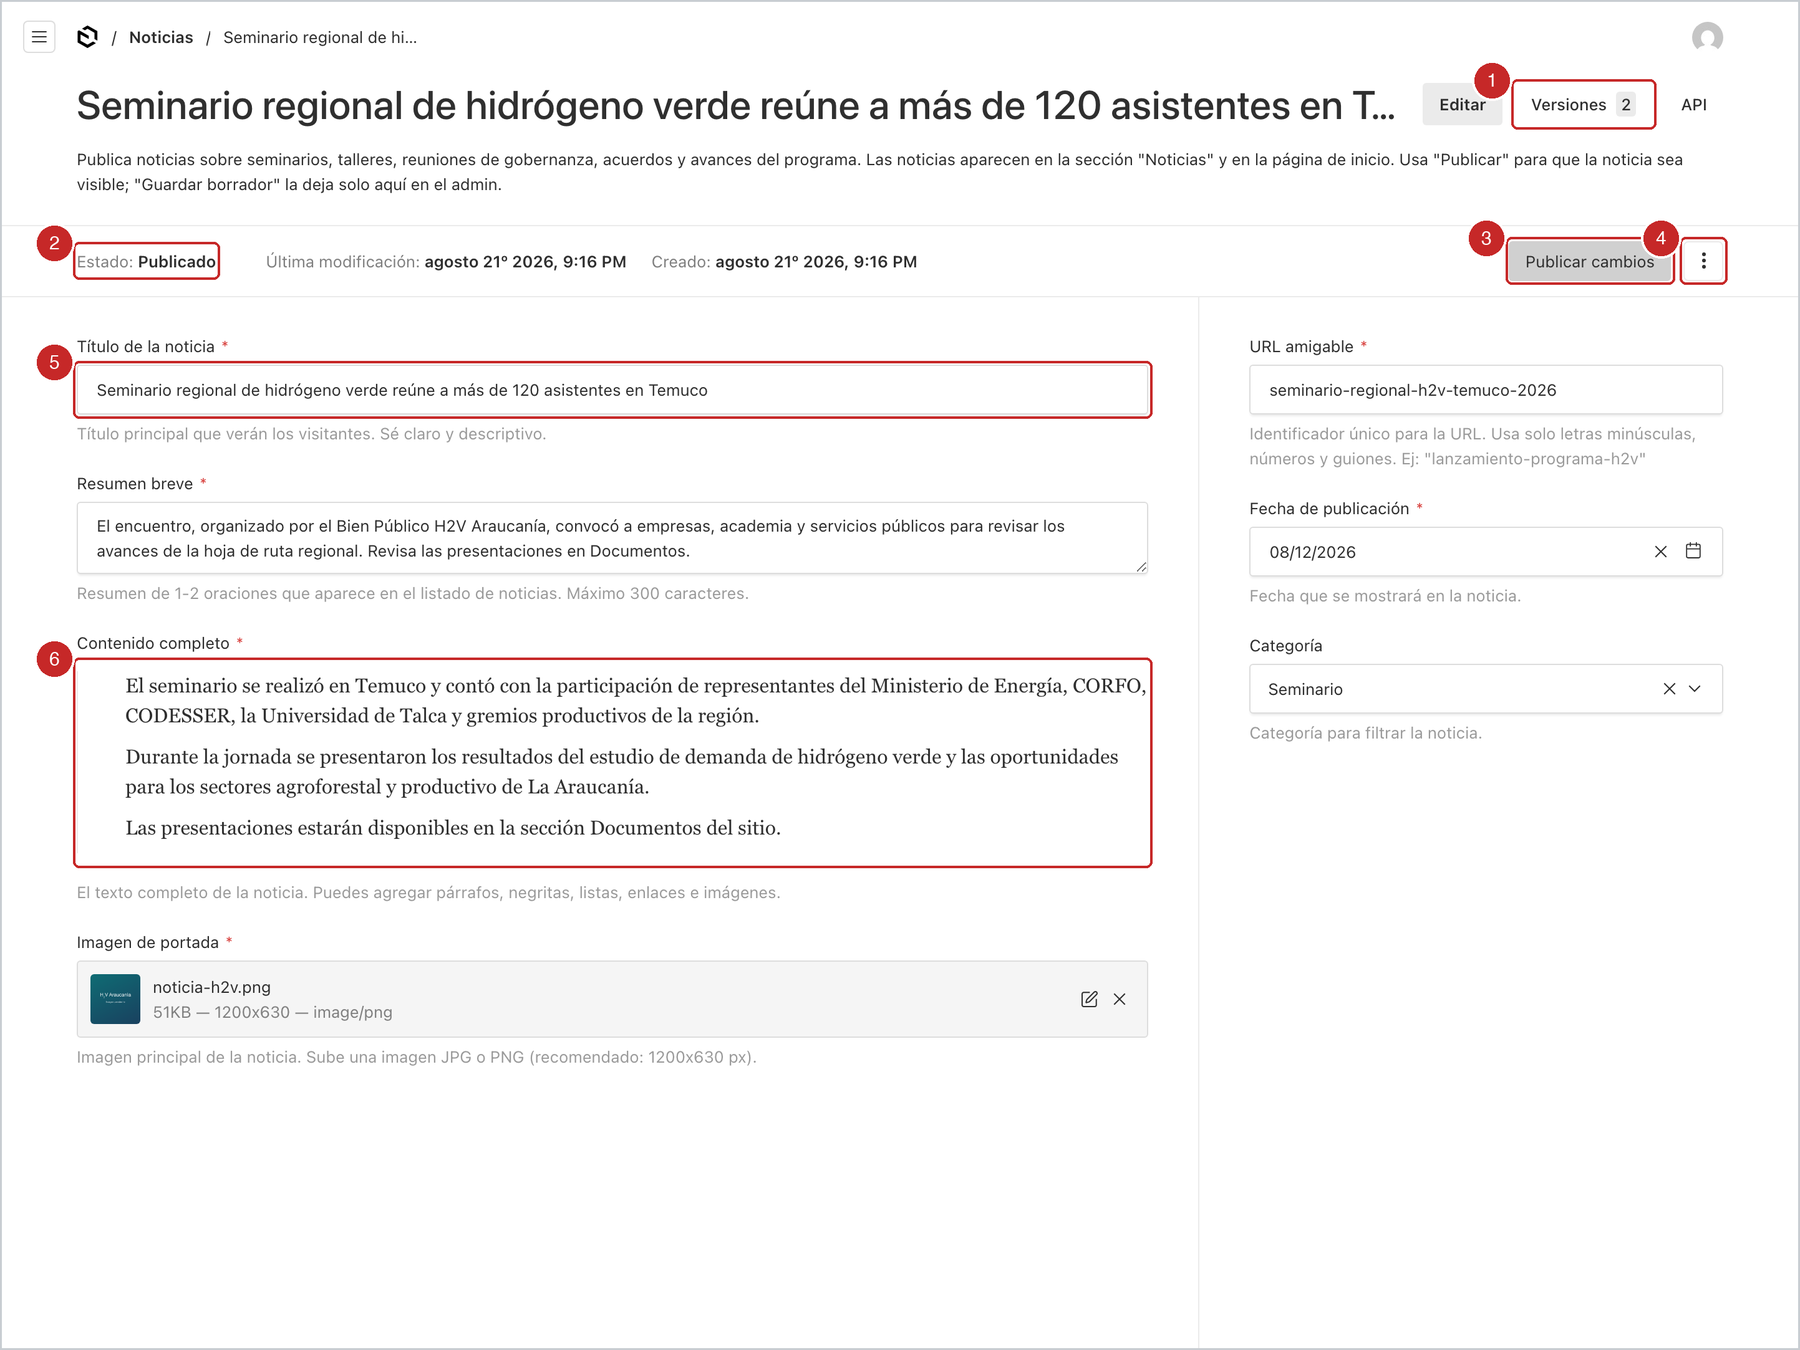
\includegraphics[width=\linewidth,keepaspectratio]{10-noticia-editar.png}
\caption{Una noticia publicada: pestaña Versiones (1), estado (2), botón Publicar cambios (3), menú de acciones (4), título (5) y contenido (6).}
\end{figure}
Cada vez que se publica queda una \textbf{versión} guardada. Si se equivocó, puede volver a una versión anterior:

\begin{enumerate}
  \item Abra la noticia o el evento y haga clic en la pestaña \textbf{Versiones} (el número indica cuántas hay).
  \item Haga clic en la versión a la que quiere volver (la lista muestra fecha y hora).
  \item Pulse \textbf{Restaurar}. Esa versión pasa a ser la actual (y queda registrada como una versión nueva, así que nunca se pierde nada).
\end{enumerate}
\begin{figure}[H]\centering
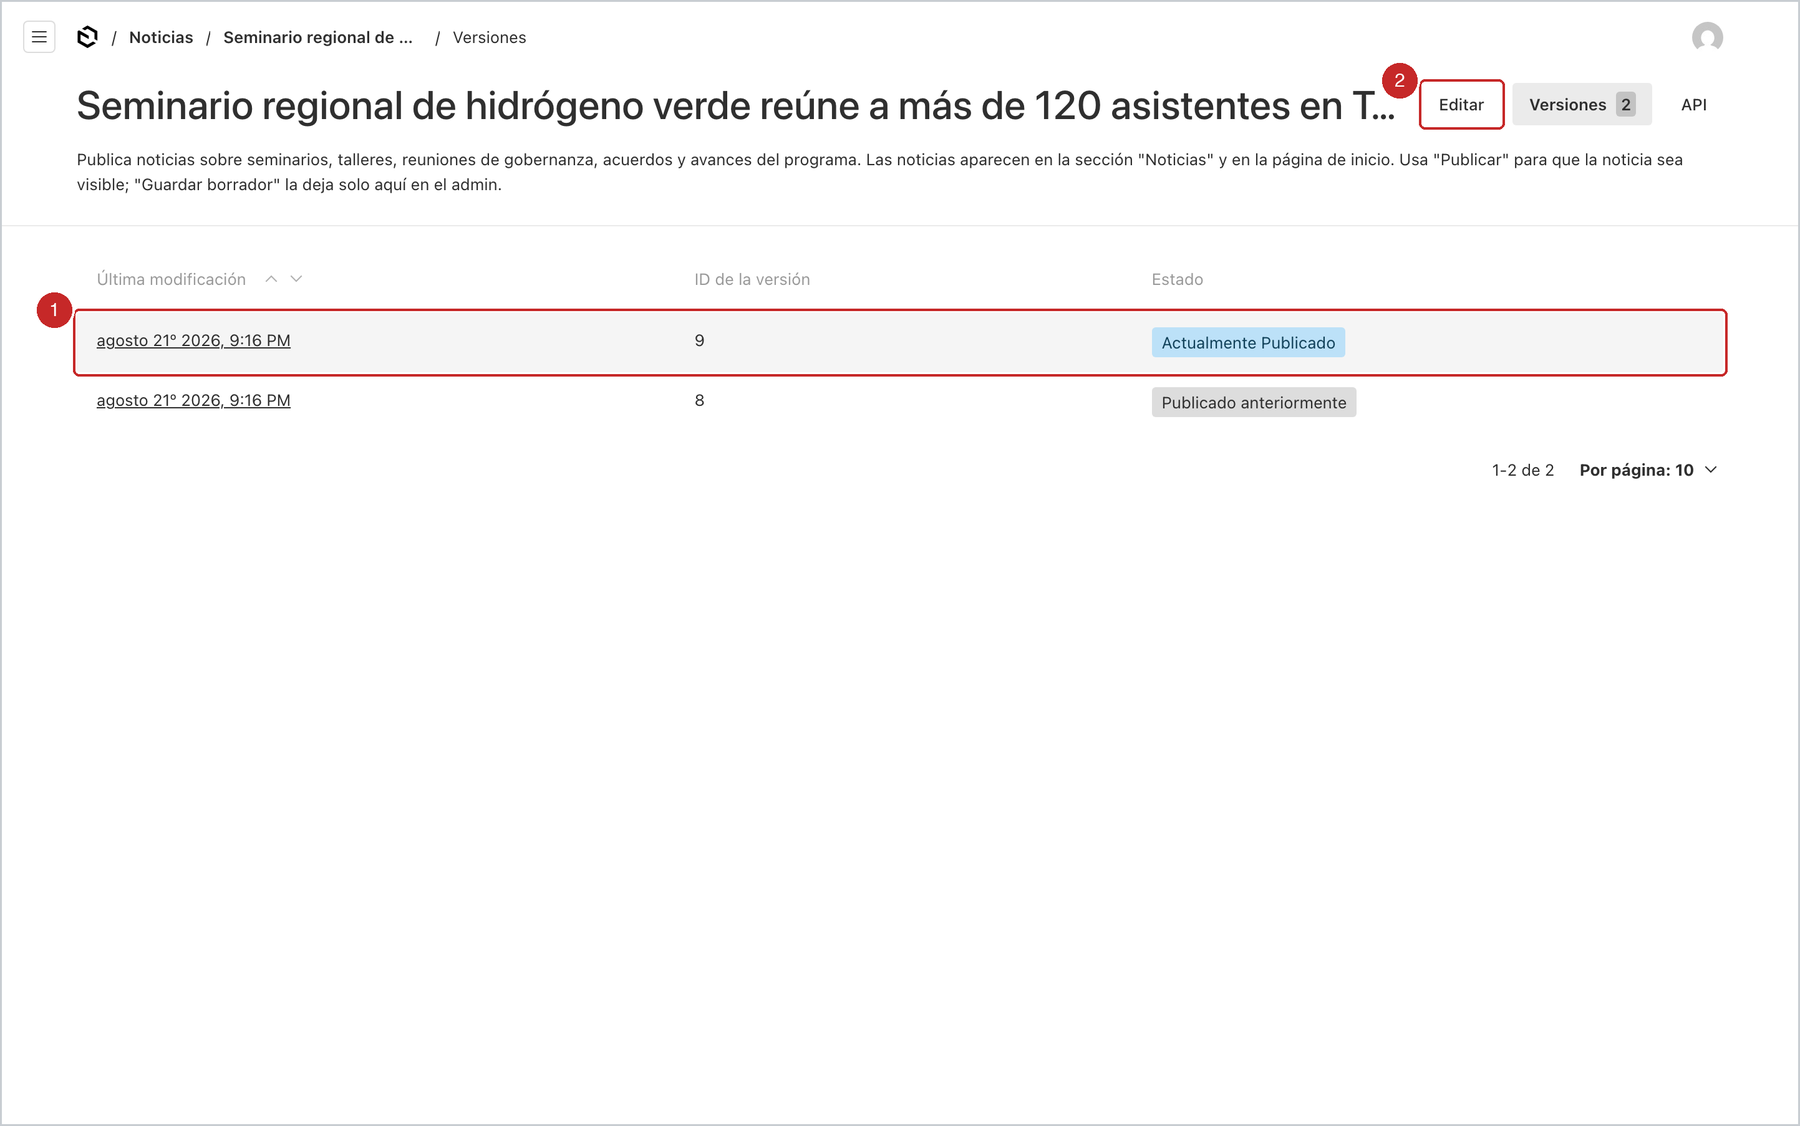
\includegraphics[width=\linewidth,keepaspectratio]{11-versiones.png}
\caption{Pestaña Versiones: cada fila (1) es un guardado con su fecha y hora.}
\end{figure}
\begin{figure}[H]\centering
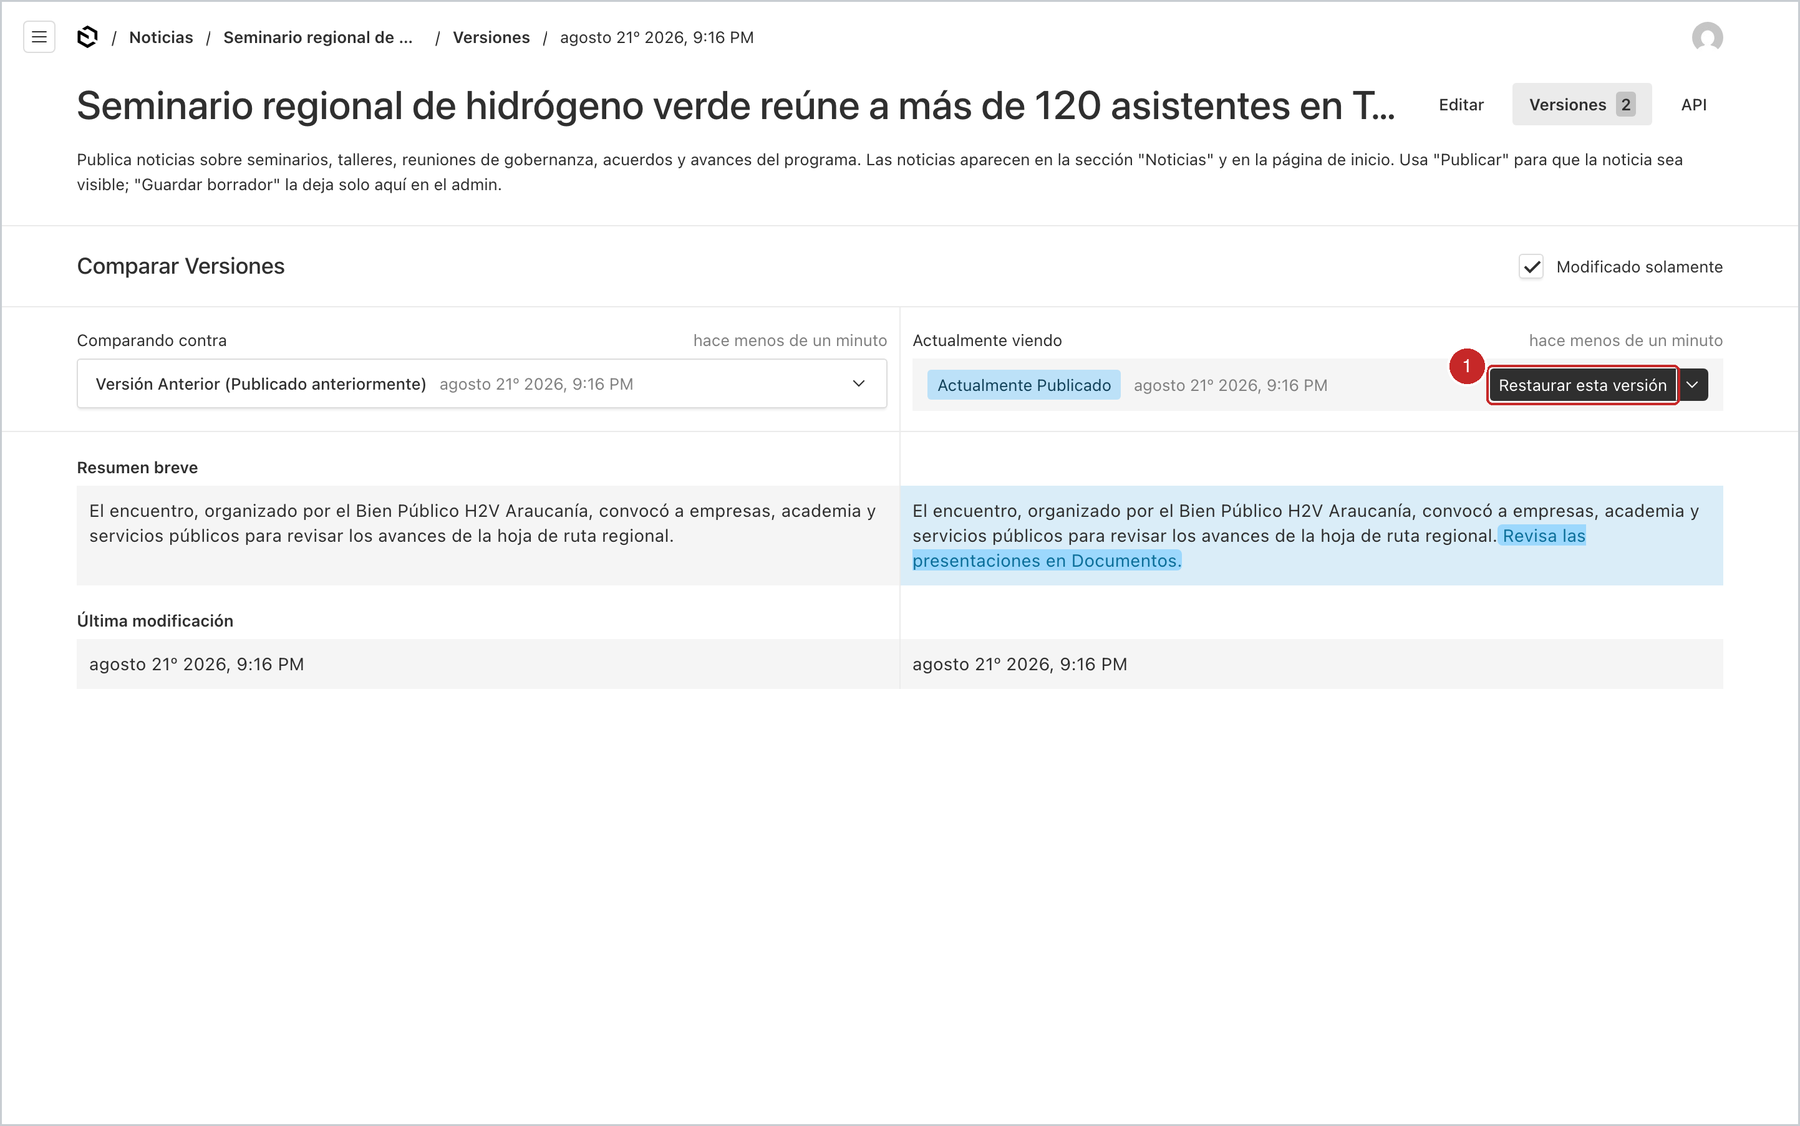
\includegraphics[width=\linewidth,keepaspectratio]{11b-version-restaurar.png}
\caption{Una versión abierta: el botón Restaurar (1) la convierte en la versión vigente.}
\end{figure}
\begin{recuadro}{cAtencion}{bAtencion}\textbf{\color{bAtencion}Atención:} los Documentos, Proyectos, Miembros y las Páginas no tienen borradores: al pulsar \textbf{Guardar} el cambio se publica de inmediato en el sitio.\end{recuadro}
\begin{recuadro}{cAtencion}{bAtencion}\textbf{\color{bAtencion}Atención:} \textbf{Eliminar es permanente} (no hay papelera). Por eso solo los Administradores pueden eliminar. Antes de eliminar algo, piense si basta con despublicarlo (dejarlo en borrador) o con editarlo.\end{recuadro}
\section{Subir imágenes y archivos}
Muchos formularios tienen un campo de archivo (por ejemplo, ''Imagen de portada'' en las noticias, ''Archivo para descargar'' en los documentos, ''Logo'' en las instituciones). Todos funcionan igual: el recuadro ofrece \textbf{Crear nuevo} (subir un archivo desde su computador), \textbf{Elegir de los existentes} (usar un archivo ya subido antes) o arrastrar y soltar el archivo desde el escritorio sobre el recuadro.

Al pulsar \textbf{Crear nuevo} se abre el cuadro de subida:

\begin{figure}[H]\centering
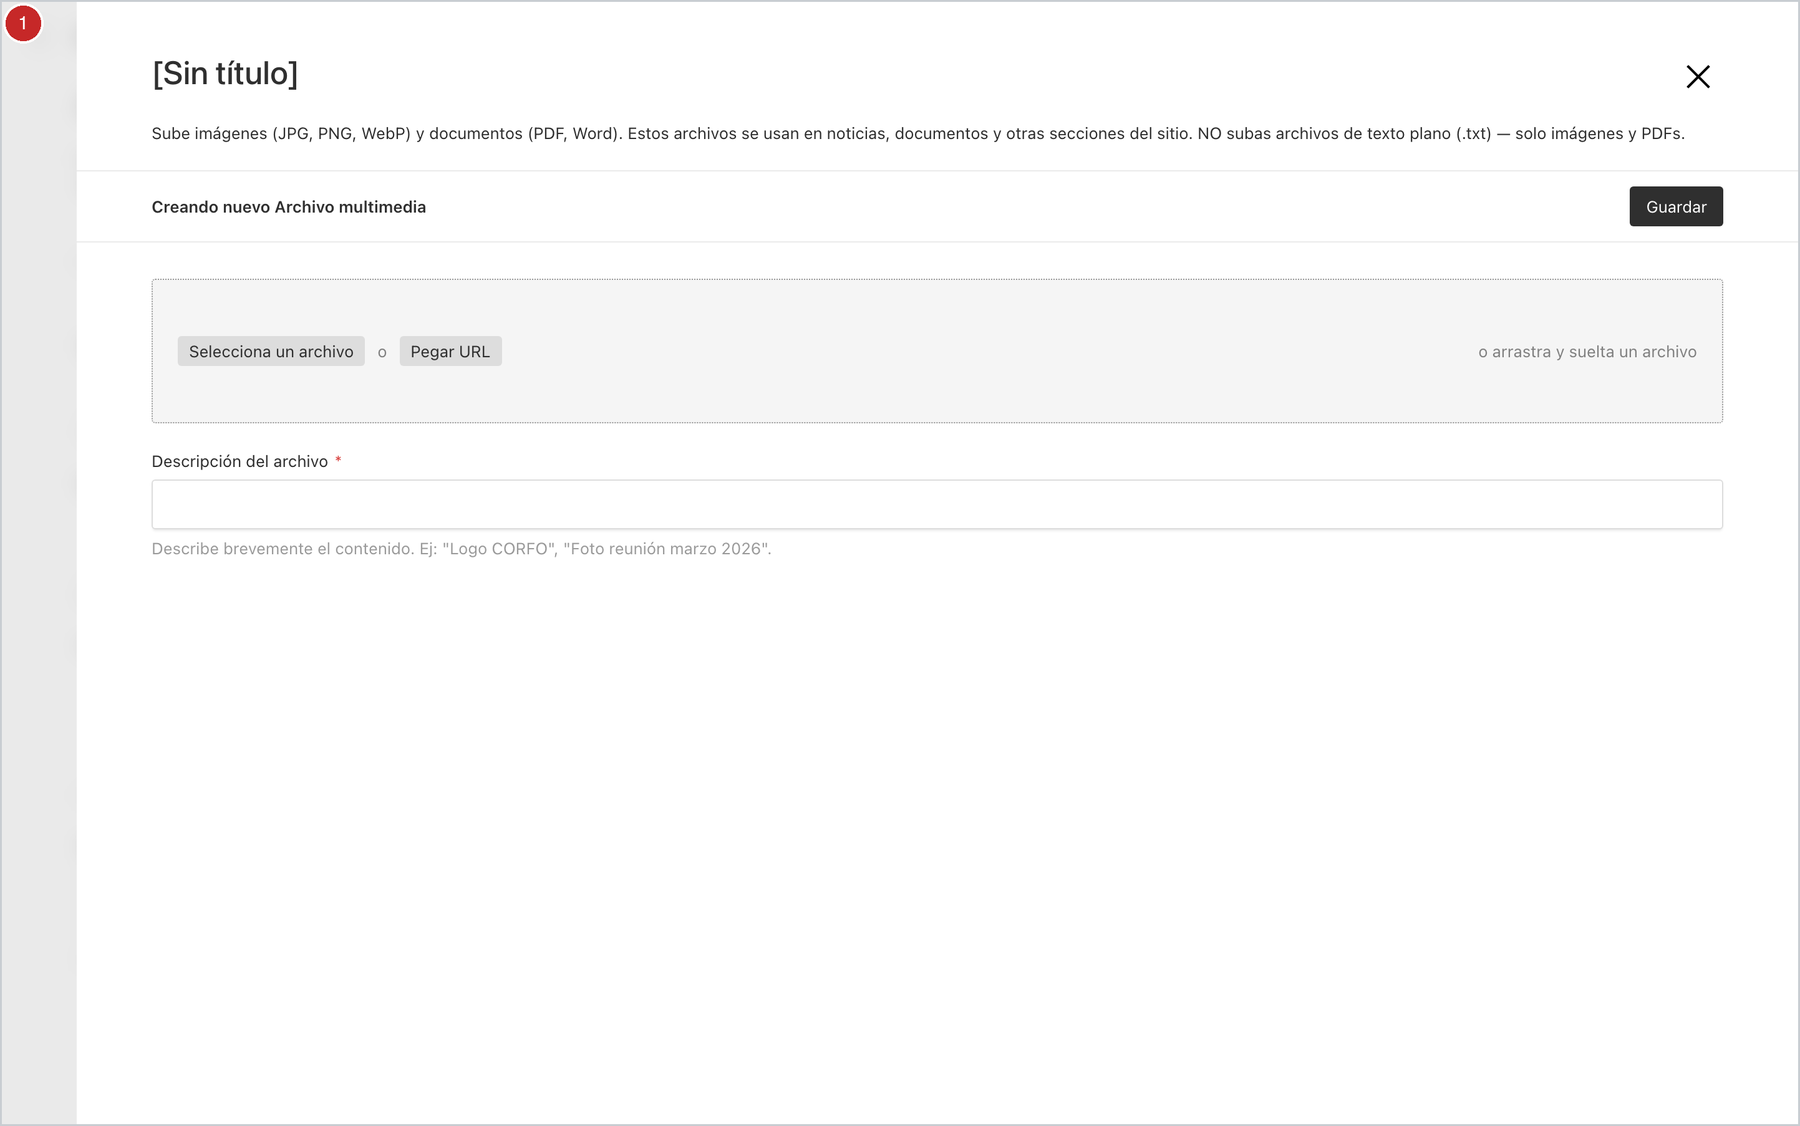
\includegraphics[width=\linewidth,keepaspectratio]{09-subir-imagen.png}
\caption{Cuadro de subida de un archivo: ''Selecciona un archivo'' abre el explorador de su computador; ''Descripción del archivo'' es obligatoria; ''Guardar'' termina la subida.}
\end{figure}
\begin{enumerate}
  \item Pulse \textbf{Selecciona un archivo} y elija el archivo en su computador (o arrástrelo al recuadro).
  \item Escriba la \textbf{Descripción del archivo} (obligatoria). Es un texto corto que dice qué es: ''Foto seminario Temuco agosto 2026'', ''Logo Seremi Energía''. Sirve para encontrar el archivo después y para las personas que usan lectores de pantalla.
  \item Pulse \textbf{Guardar}. El archivo queda subido y asociado al campo.
\end{enumerate}
\begin{longtable}{>{\raggedright\arraybackslash}p{0.143\textwidth}>{\raggedright\arraybackslash}p{0.271\textwidth}>{\raggedright\arraybackslash}p{0.516\textwidth}}
\rowcolor{h2vazul}\textbf{\color{white}Tipo de archivo} & \textbf{\color{white}Formatos aceptados} & \textbf{\color{white}Recomendaciones} \\
\endfirsthead
\rowcolor{h2vazul}\textbf{\color{white}Tipo de archivo} & \textbf{\color{white}Formatos aceptados} & \textbf{\color{white}Recomendaciones} \\
\endhead
Imágenes & JPG, PNG, WebP, GIF, SVG & Portada de noticia: 1200 x 630 píxeles. Fotos de personas: cuadradas, mínimo 200 x 200. Fotos de galería: horizontales. \\ \midrule
\rowcolor{filaalt}Documentos & PDF, Word (.docx), PowerPoint (.pptx), Excel (.xlsx) & Prefiera PDF para lo que el público descarga. \\ \bottomrule
\end{longtable}
\begin{recuadro}{cConsejo}{bConsejo}\textbf{\color{bConsejo}Consejo:} antes de subir un archivo, póngale un nombre claro en su computador (por ejemplo \texttt{seminario-temuco-2026.pdf}). Las imágenes muy pesadas (más de 5 MB) hacen lenta la página: reduzca el tamaño antes de subirlas.\end{recuadro}
Todos los archivos subidos quedan también en \textbf{Sistema $\rightarrow$ Archivos multimedia}, donde se pueden buscar y reutilizar (vea ''Archivos multimedia'' en el capítulo de tareas).

\section{El editor de texto}
El contenido de las noticias, la descripción de los eventos y algunos textos largos de las páginas se escriben en un editor de texto enriquecido, parecido a un procesador de texto sencillo. Funciona así:

\begin{itemize}
  \item \textbf{Escriba} directamente donde dice ''Comience a escribir, o presione '/' para comandos''.
  \item \textbf{Para dar formato} (negrita, cursiva, subrayado, enlace, alineación), \textbf{seleccione el texto con el ratón}: aparece una barra flotante con los botones.
  \item \textbf{Para insertar un elemento} (un título, una lista, una cita, una imagen), escriba el símbolo \textbf{/} al comienzo de una línea vacía, o pulse el botón \textbf{+} que aparece al lado izquierdo de la línea: se abre un menú con las opciones; elija una.
\end{itemize}
\begin{figure}[H]\centering
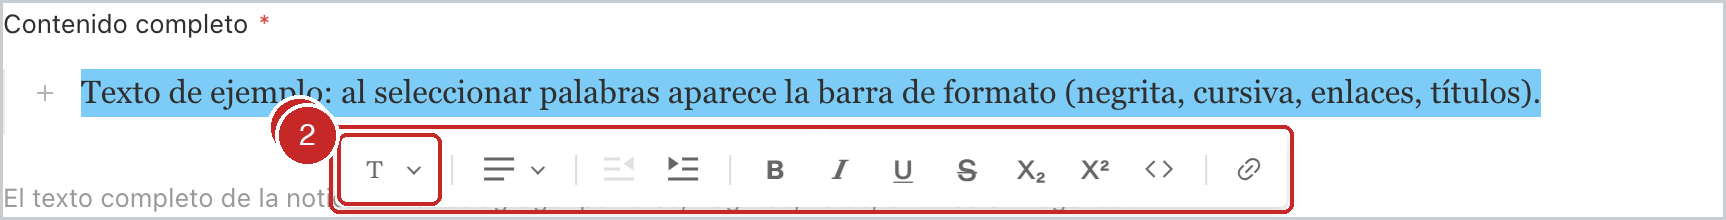
\includegraphics[width=\linewidth,keepaspectratio]{07-editor-barra.png}
\caption{Barra flotante que aparece al seleccionar texto (1): el primer desplegable (2) convierte el párrafo en título; siguen alineación, sangría, negrita, cursiva, subrayado, tachado, subíndice, superíndice, código y enlace.}
\end{figure}
\begin{figure}[H]\centering
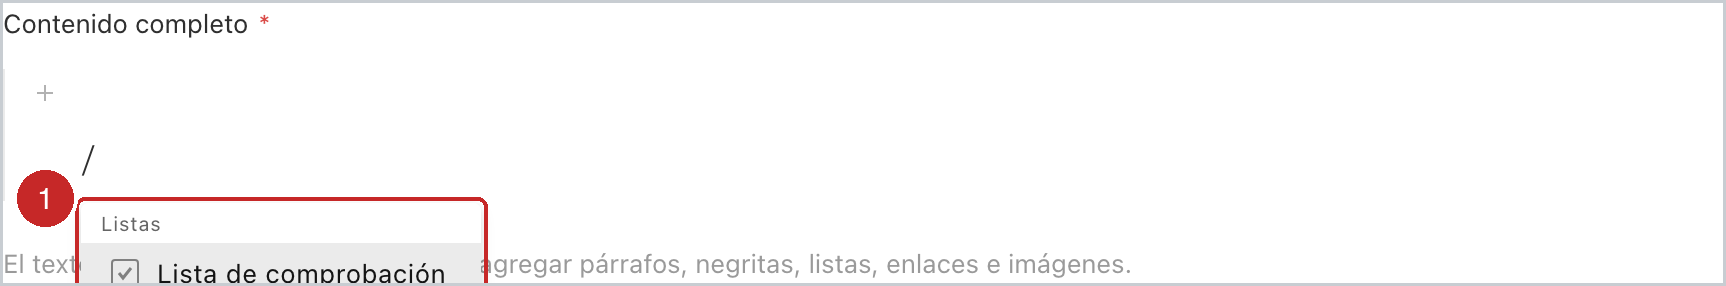
\includegraphics[width=\linewidth,keepaspectratio]{08-editor-slash.png}
\caption{Menú de comandos que aparece al escribir ''/'' en una línea vacía: títulos, listas (con viñetas, numeradas, de comprobación), cita, enlaces y subida de imagen.}
\end{figure}
Acciones más comunes:

\begin{longtable}{>{\raggedright\arraybackslash}p{0.234\textwidth}>{\raggedright\arraybackslash}p{0.696\textwidth}}
\rowcolor{h2vazul}\textbf{\color{white}Quiero...} & \textbf{\color{white}Cómo} \\
\endfirsthead
\rowcolor{h2vazul}\textbf{\color{white}Quiero...} & \textbf{\color{white}Cómo} \\
\endhead
Poner negrita o cursiva & Seleccionar el texto y pulsar \textbf{B} o \textbf{I} en la barra flotante \\ \midrule
\rowcolor{filaalt}Poner un subtítulo dentro del texto & Escribir ''/'' y elegir \textbf{Título 2} (o seleccionar el texto y usar el primer desplegable de la barra flotante) \\ \midrule
Hacer una lista & Escribir ''/'' y elegir \textbf{Lista con viñetas} o \textbf{Lista numerada} \\ \midrule
\rowcolor{filaalt}Poner un enlace a otra página web & Seleccionar el texto y pulsar el icono de enlace (el último de la barra); pegar la dirección web completa, con \url{https://} \\ \midrule
Insertar una imagen dentro del texto & Escribir ''/'' y elegir la opción de subir/insertar imagen; subir o elegir una existente \\ \midrule
\rowcolor{filaalt}Deshacer & Ctrl + Z (Cmd + Z en Mac) \\ \bottomrule
\end{longtable}
\begin{recuadro}{cConsejo}{bConsejo}\textbf{\color{bConsejo}Consejo:} si pega texto desde Word, el editor conserva párrafos, negritas y listas, pero no colores ni tipografías (a propósito: el sitio aplica su propio diseño).\end{recuadro}
\chapter{Tareas frecuentes, paso a paso}
\section{Publicar una noticia}
Las noticias aparecen en la sección \textbf{Noticias} del sitio y las más recientes se muestran también en la portada.

\begin{enumerate}
  \item En el menú lateral, haga clic en \textbf{Noticias} (grupo Contenido).
  \item Pulse \textbf{Crear nuevo} (arriba a la derecha de la lista). Se abre el formulario vacío, que ya está en estado Borrador y se guarda solo.
  \item Complete los campos (vea la figura del formulario en el capítulo anterior):
\end{enumerate}
\begin{longtable}{>{\raggedright\arraybackslash}p{0.196\textwidth}>{\raggedright\arraybackslash}p{0.579\textwidth}>{\raggedright\arraybackslash}p{0.155\textwidth}}
\rowcolor{h2vazul}\textbf{\color{white}Campo} & \textbf{\color{white}Qué escribir} & \textbf{\color{white}Obligatorio} \\
\endfirsthead
\rowcolor{h2vazul}\textbf{\color{white}Campo} & \textbf{\color{white}Qué escribir} & \textbf{\color{white}Obligatorio} \\
\endhead
\textbf{Título de la noticia} & El titular que verán los visitantes. Máximo 120 caracteres. Ejemplo: ''Seminario regional de hidrógeno verde reúne a más de 120 asistentes en Temuco''. & Sí \\ \midrule
\rowcolor{filaalt}\textbf{Resumen breve} & Una o dos oraciones que aparecen en el listado de noticias. Máximo 300 caracteres. & Sí \\ \midrule
\textbf{Contenido completo} & El texto completo. Use el editor: párrafos, subtítulos, negritas, listas, enlaces e imágenes. & Sí \\ \midrule
\rowcolor{filaalt}\textbf{Imagen de portada} & Una imagen JPG o PNG (recomendado 1200 x 630 píxeles). Aparece en el listado y arriba de la noticia. & Sí \\ \midrule
\textbf{URL amigable} (barra lateral) & El identificador que aparece en la dirección web de la noticia. Solo letras minúsculas, números y guiones, sin espacios ni tildes. Ejemplo: \texttt{seminario-regional-h2v-temuco-2026}. Debe ser único. & Sí \\ \midrule
\rowcolor{filaalt}\textbf{Fecha de publicación} (barra lateral) & La fecha que se mostrará en la noticia. Elíjala en el calendario. & Sí \\ \midrule
\textbf{Categoría} (barra lateral) & Seminario, Taller, Gobernanza, Acuerdo, Proyecto o General. Sirve para filtrar. & No \\ \bottomrule
\end{longtable}
\begin{enumerate}[start=4]
  \item Pulse \textbf{Publicar cambios}.
\end{enumerate}
\begin{recuadro}{cResultado}{bResultado}\textbf{\color{bResultado}Resultado:} la barra de estado cambia a ''Publicado''. Abra el sitio público, entre a Noticias y recargue: la noticia aparece primera. En la portada aparece entre las últimas noticias.\end{recuadro}
\begin{figure}[H]\centering
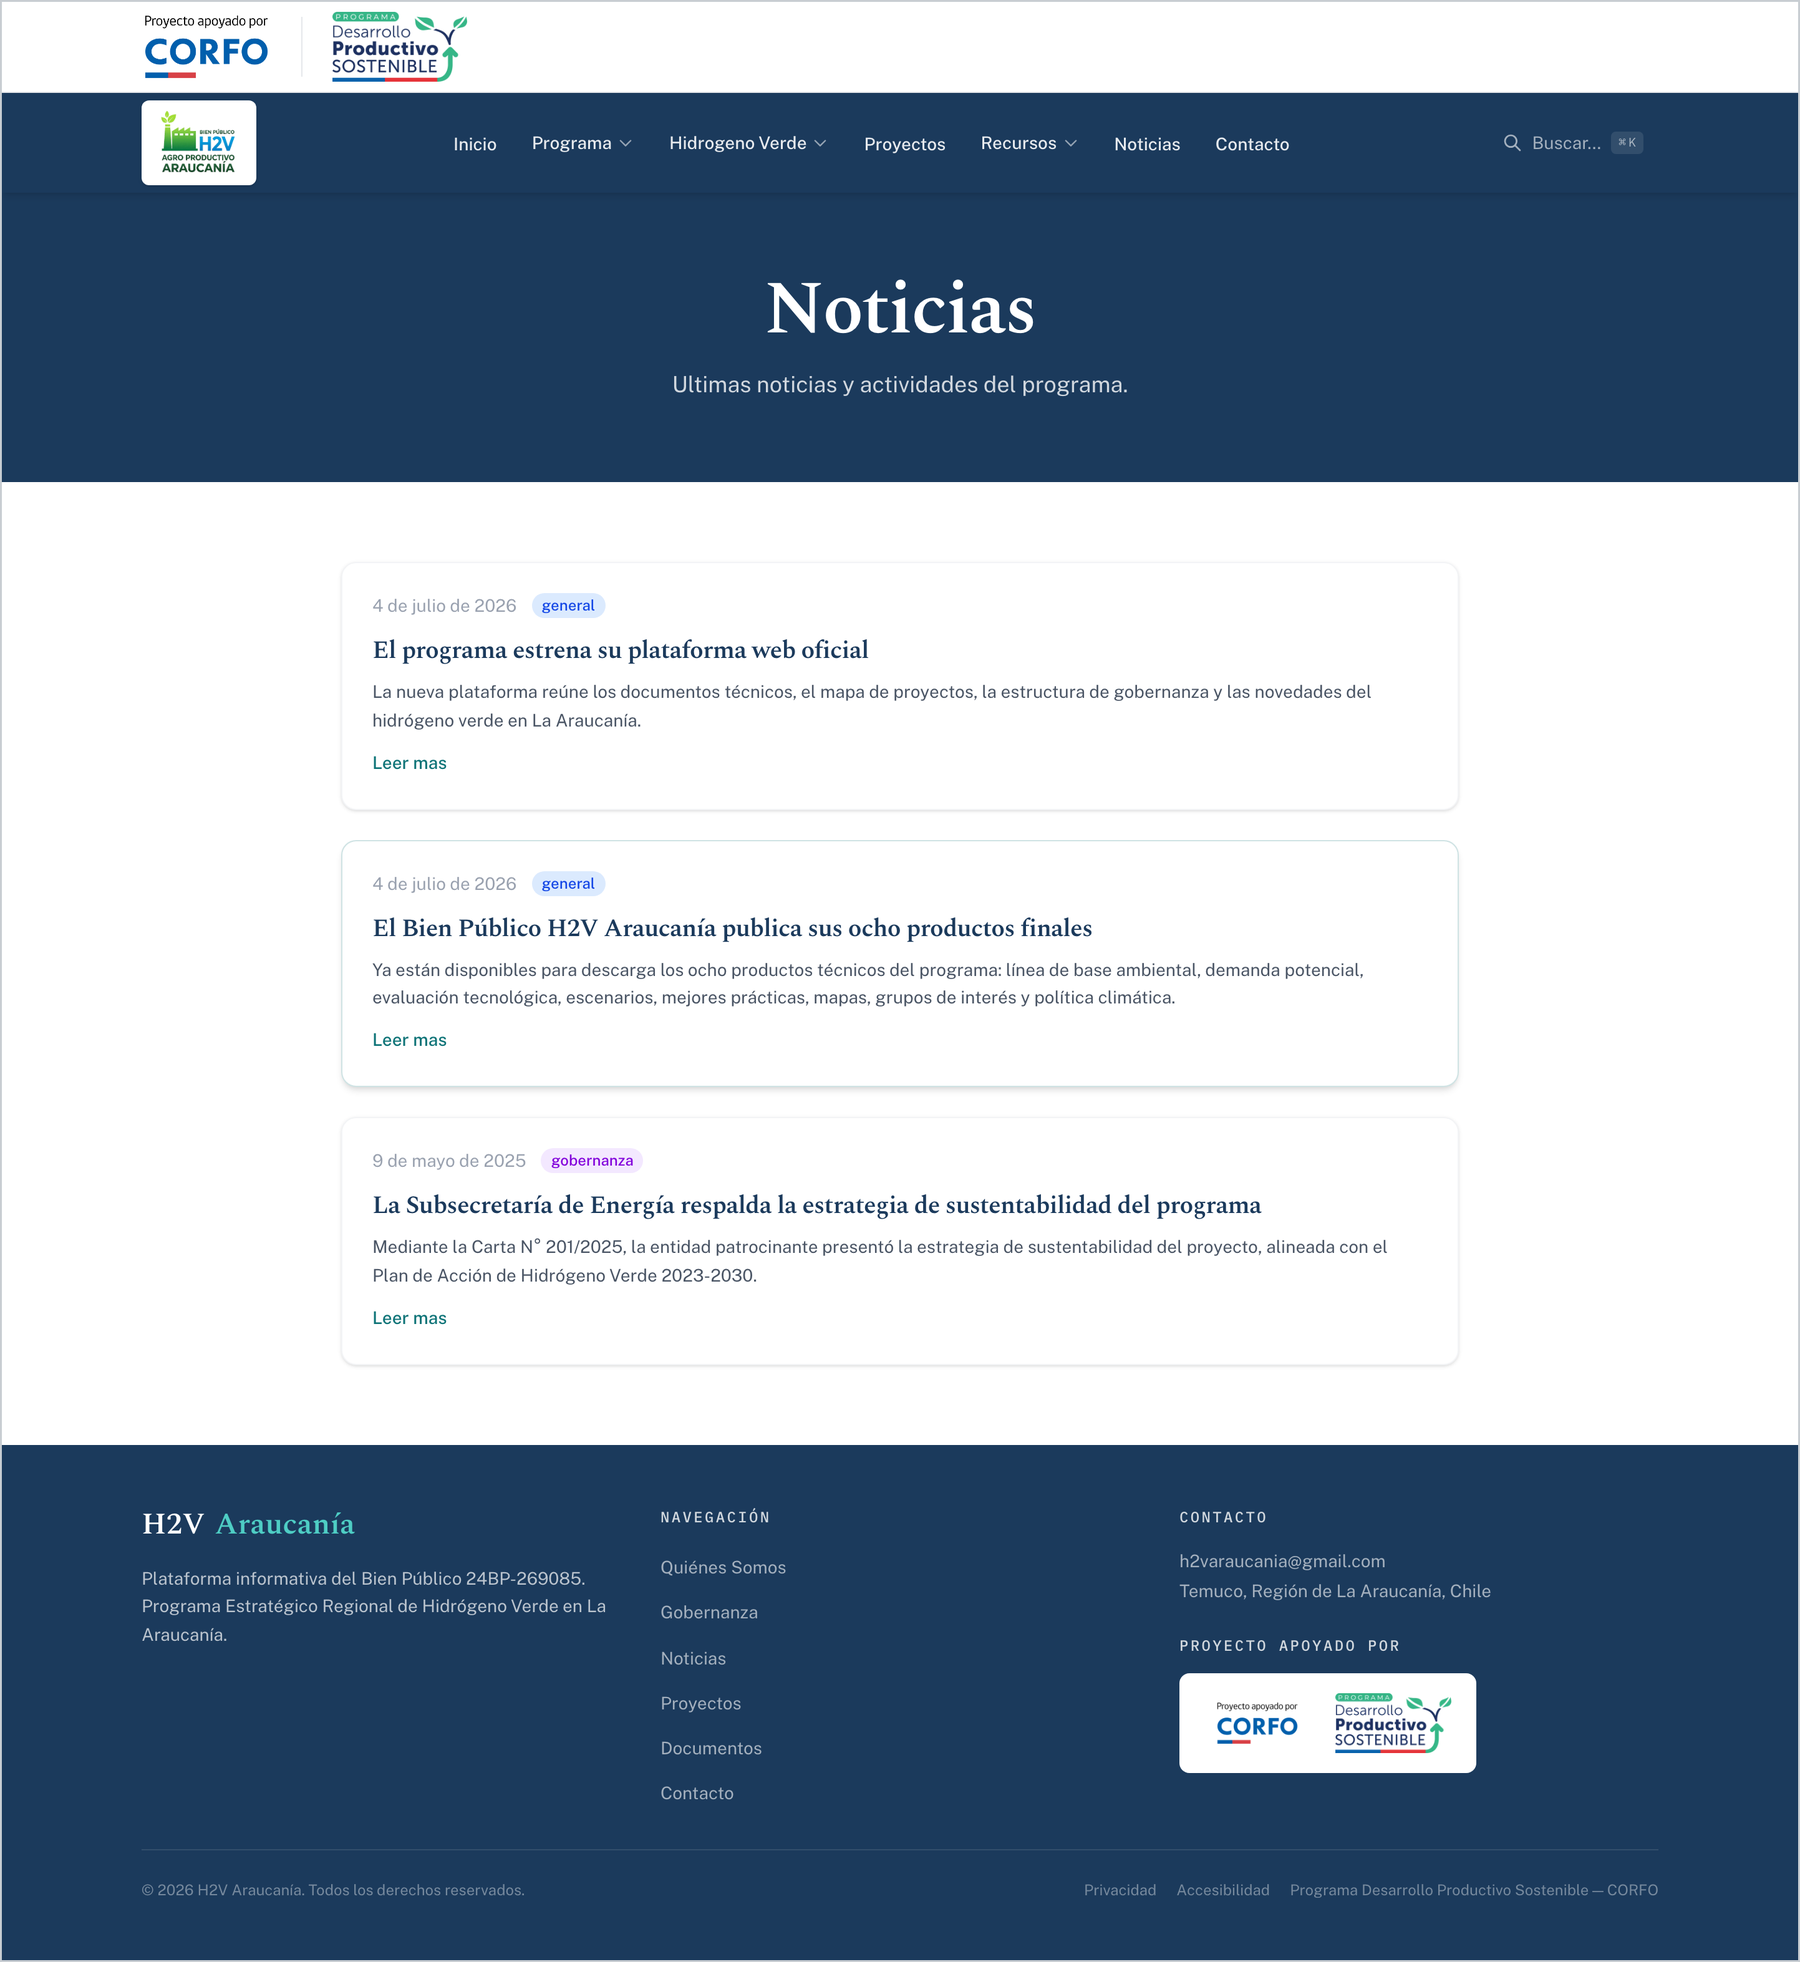
\includegraphics[width=\linewidth,keepaspectratio]{43-web-noticias.png}
\caption{Así se ve la sección Noticias del sitio público.}
\end{figure}
\begin{figure}[H]\centering
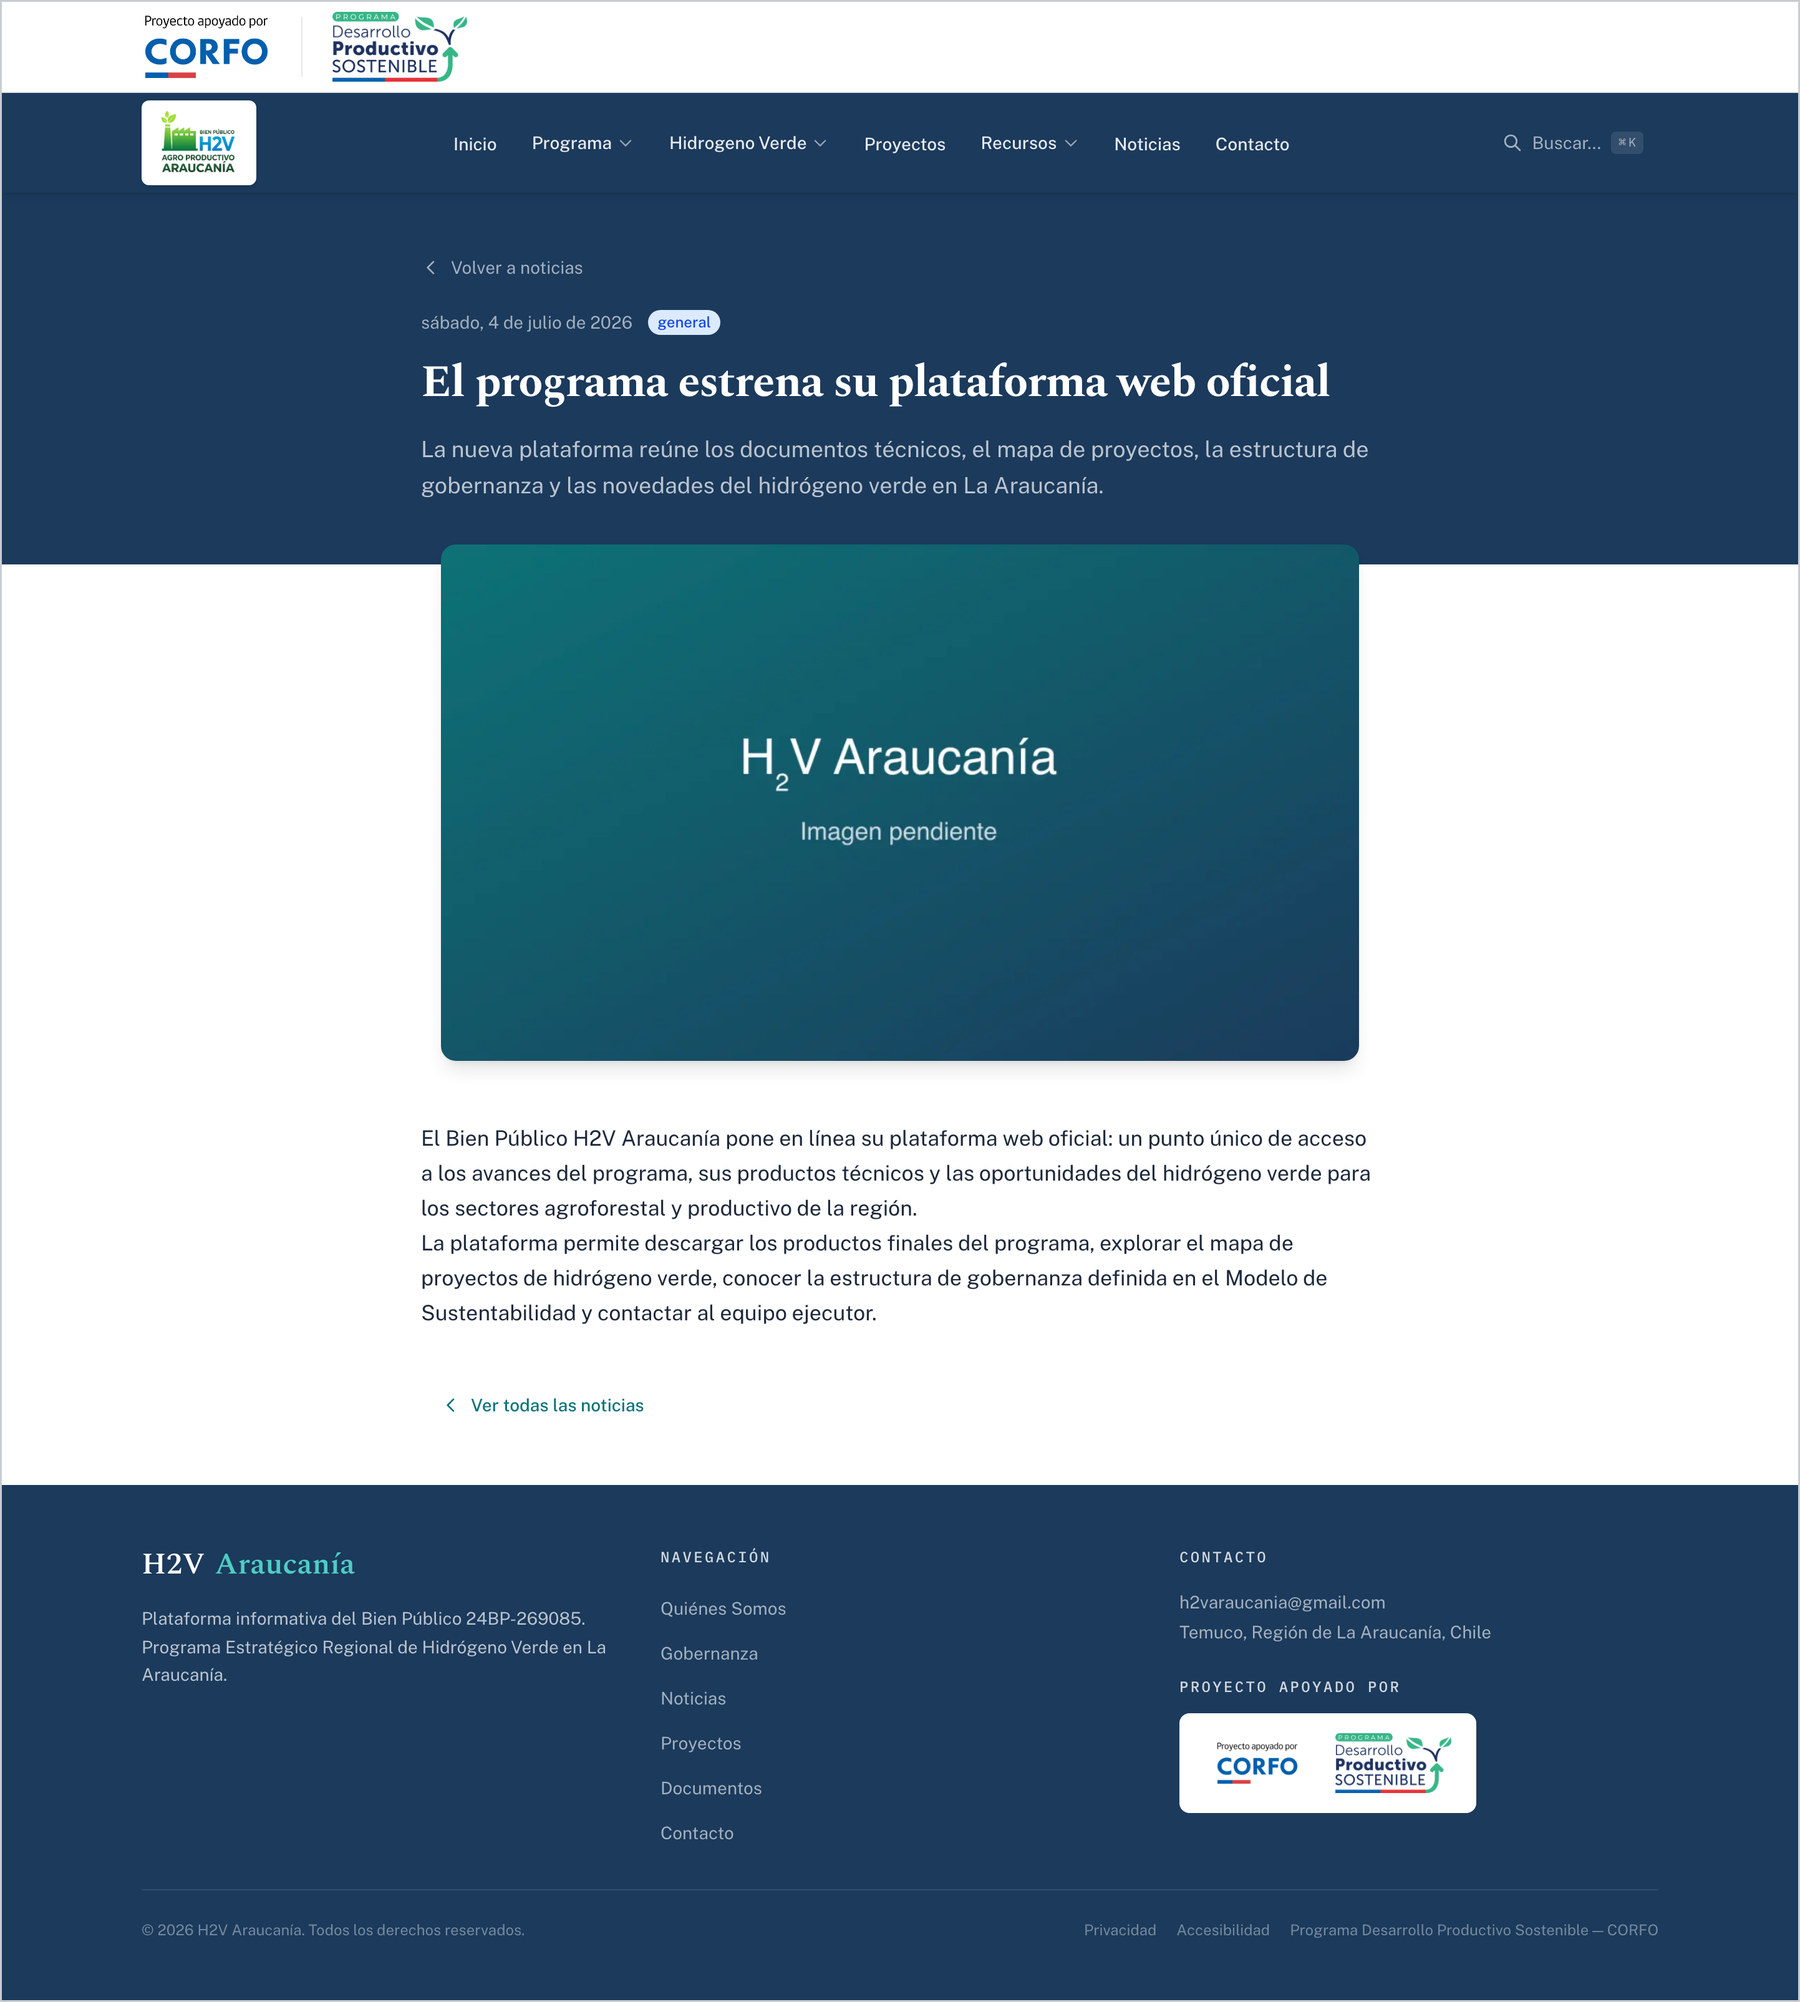
\includegraphics[width=\linewidth,keepaspectratio]{44-web-noticia-detalle.png}
\caption{Así se ve una noticia abierta: imagen de portada, fecha, categoría y contenido.}
\end{figure}
\begin{recuadro}{cAtencion}{bAtencion}\textbf{\color{bAtencion}Atención:} si la noticia no aparece en el sitio, casi siempre es porque quedó en \textbf{Borrador}: ábrala y pulse \textbf{Publicar cambios}. Si el panel marca en rojo la URL amigable con un mensaje de valor duplicado, cambie el texto (ya existe otra noticia con esa URL).\end{recuadro}
\section{Editar, despublicar o eliminar una noticia}
\begin{itemize}
  \item \textbf{Editar}: en la lista de Noticias haga clic en el título, modifique lo que necesite y pulse \textbf{Publicar cambios}. Hasta que lo pulse, el sitio sigue mostrando la versión anterior.
  \item \textbf{Despublicar} (que deje de verse sin borrarla): abra la noticia, pulse el botón de tres puntos junto a ''Publicar cambios'' y elija la opción de \textbf{despublicar} (o restaure una versión en borrador). La noticia queda en el panel como borrador.
  \item \textbf{Eliminar} (solo Administradores): abra la noticia, botón de tres puntos, \textbf{Eliminar}, y confirme. Es permanente.
  \item \textbf{Duplicar}: el mismo menú tiene \textbf{Duplicar}, útil para crear una noticia parecida a otra.
\end{itemize}
\section{Crear un evento}
Los eventos aparecen en \textbf{Recursos $\rightarrow$ Eventos} del sitio. Funcionan igual que las noticias (borrador automático y botón Publicar cambios).

\begin{enumerate}
  \item Menú lateral $\rightarrow$ \textbf{Eventos} $\rightarrow$ \textbf{Crear nuevo}.
  \item Complete:
\end{enumerate}
\begin{longtable}{>{\raggedright\arraybackslash}p{0.250\textwidth}>{\raggedright\arraybackslash}p{0.526\textwidth}>{\raggedright\arraybackslash}p{0.155\textwidth}}
\rowcolor{h2vazul}\textbf{\color{white}Campo} & \textbf{\color{white}Qué escribir} & \textbf{\color{white}Obligatorio} \\
\endfirsthead
\rowcolor{h2vazul}\textbf{\color{white}Campo} & \textbf{\color{white}Qué escribir} & \textbf{\color{white}Obligatorio} \\
\endhead
\textbf{Nombre del evento} & Ejemplo: ''Taller de capacitación: H2V para el sector forestal''. Máximo 120 caracteres. & Sí \\ \midrule
\rowcolor{filaalt}\textbf{Descripción} & Programa, expositores, objetivos, público. Use el editor de texto. & Sí \\ \midrule
\textbf{Fecha de inicio} (barra lateral) & Día en que comienza. & Sí \\ \midrule
\rowcolor{filaalt}\textbf{Fecha de término} (barra lateral) & Solo si dura más de un día. & No \\ \midrule
\textbf{Lugar} & Dirección física u ''Online vía Zoom''. Máximo 100 caracteres. & Sí \\ \midrule
\rowcolor{filaalt}\textbf{Tipo de evento} (barra lateral) & Seminario, Taller, Feria, Reunión, Capacitación u Otro. & No \\ \midrule
\textbf{Imagen o afiche} & Imagen promocional. & No \\ \midrule
\rowcolor{filaalt}\textbf{Enlace de inscripción} & Dirección web del formulario de inscripción (Google Forms, Eventbrite...). & No \\ \bottomrule
\end{longtable}
\begin{enumerate}[start=3]
  \item Pulse \textbf{Publicar cambios}.
\end{enumerate}
\begin{figure}[H]\centering
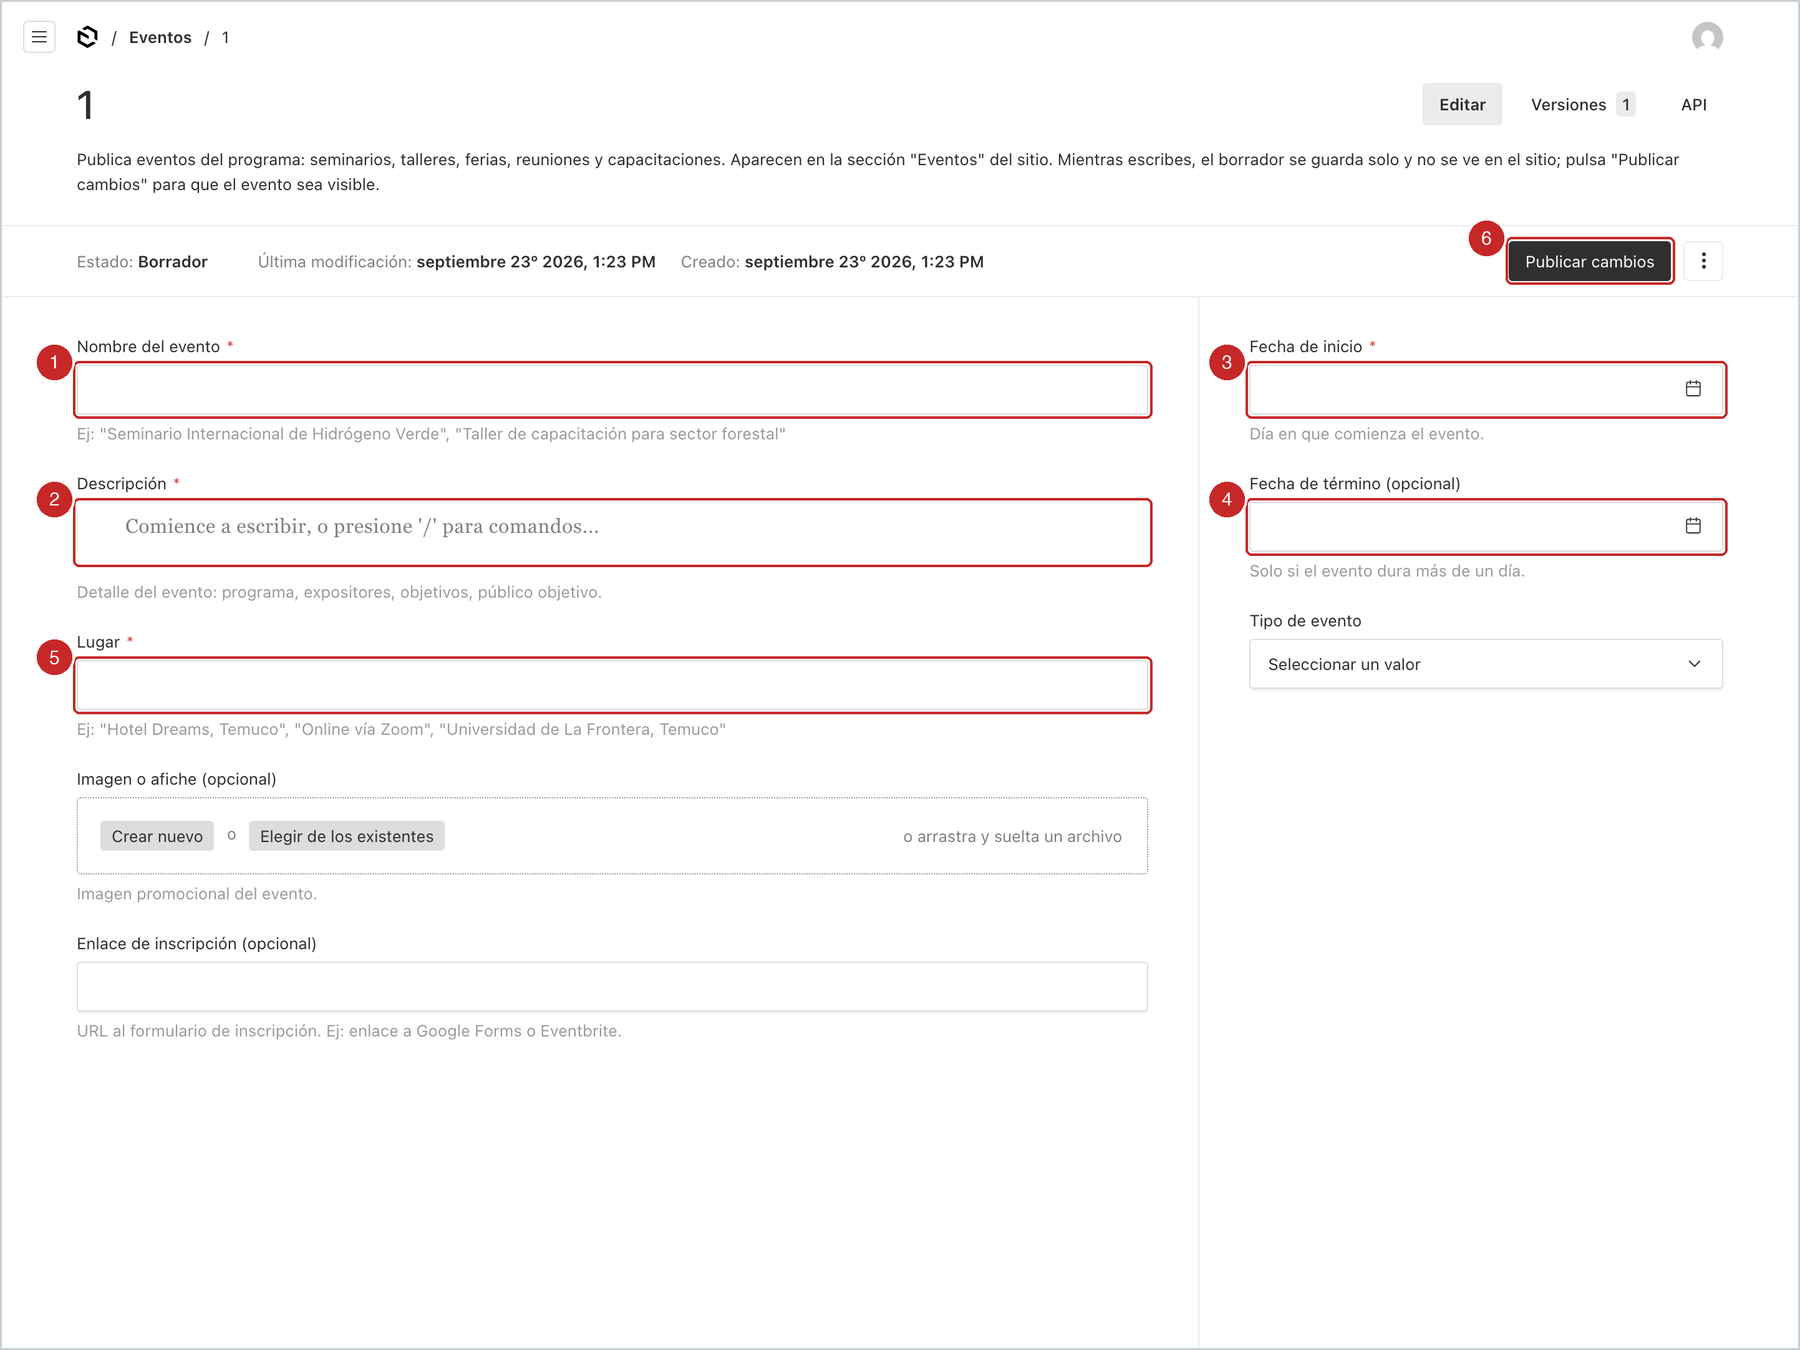
\includegraphics[width=\linewidth,keepaspectratio]{15-evento-crear.png}
\caption{Formulario de un evento nuevo: nombre (1), descripción (2), fechas (3 y 4), lugar (5) y Publicar cambios (6).}
\end{figure}
\begin{figure}[H]\centering
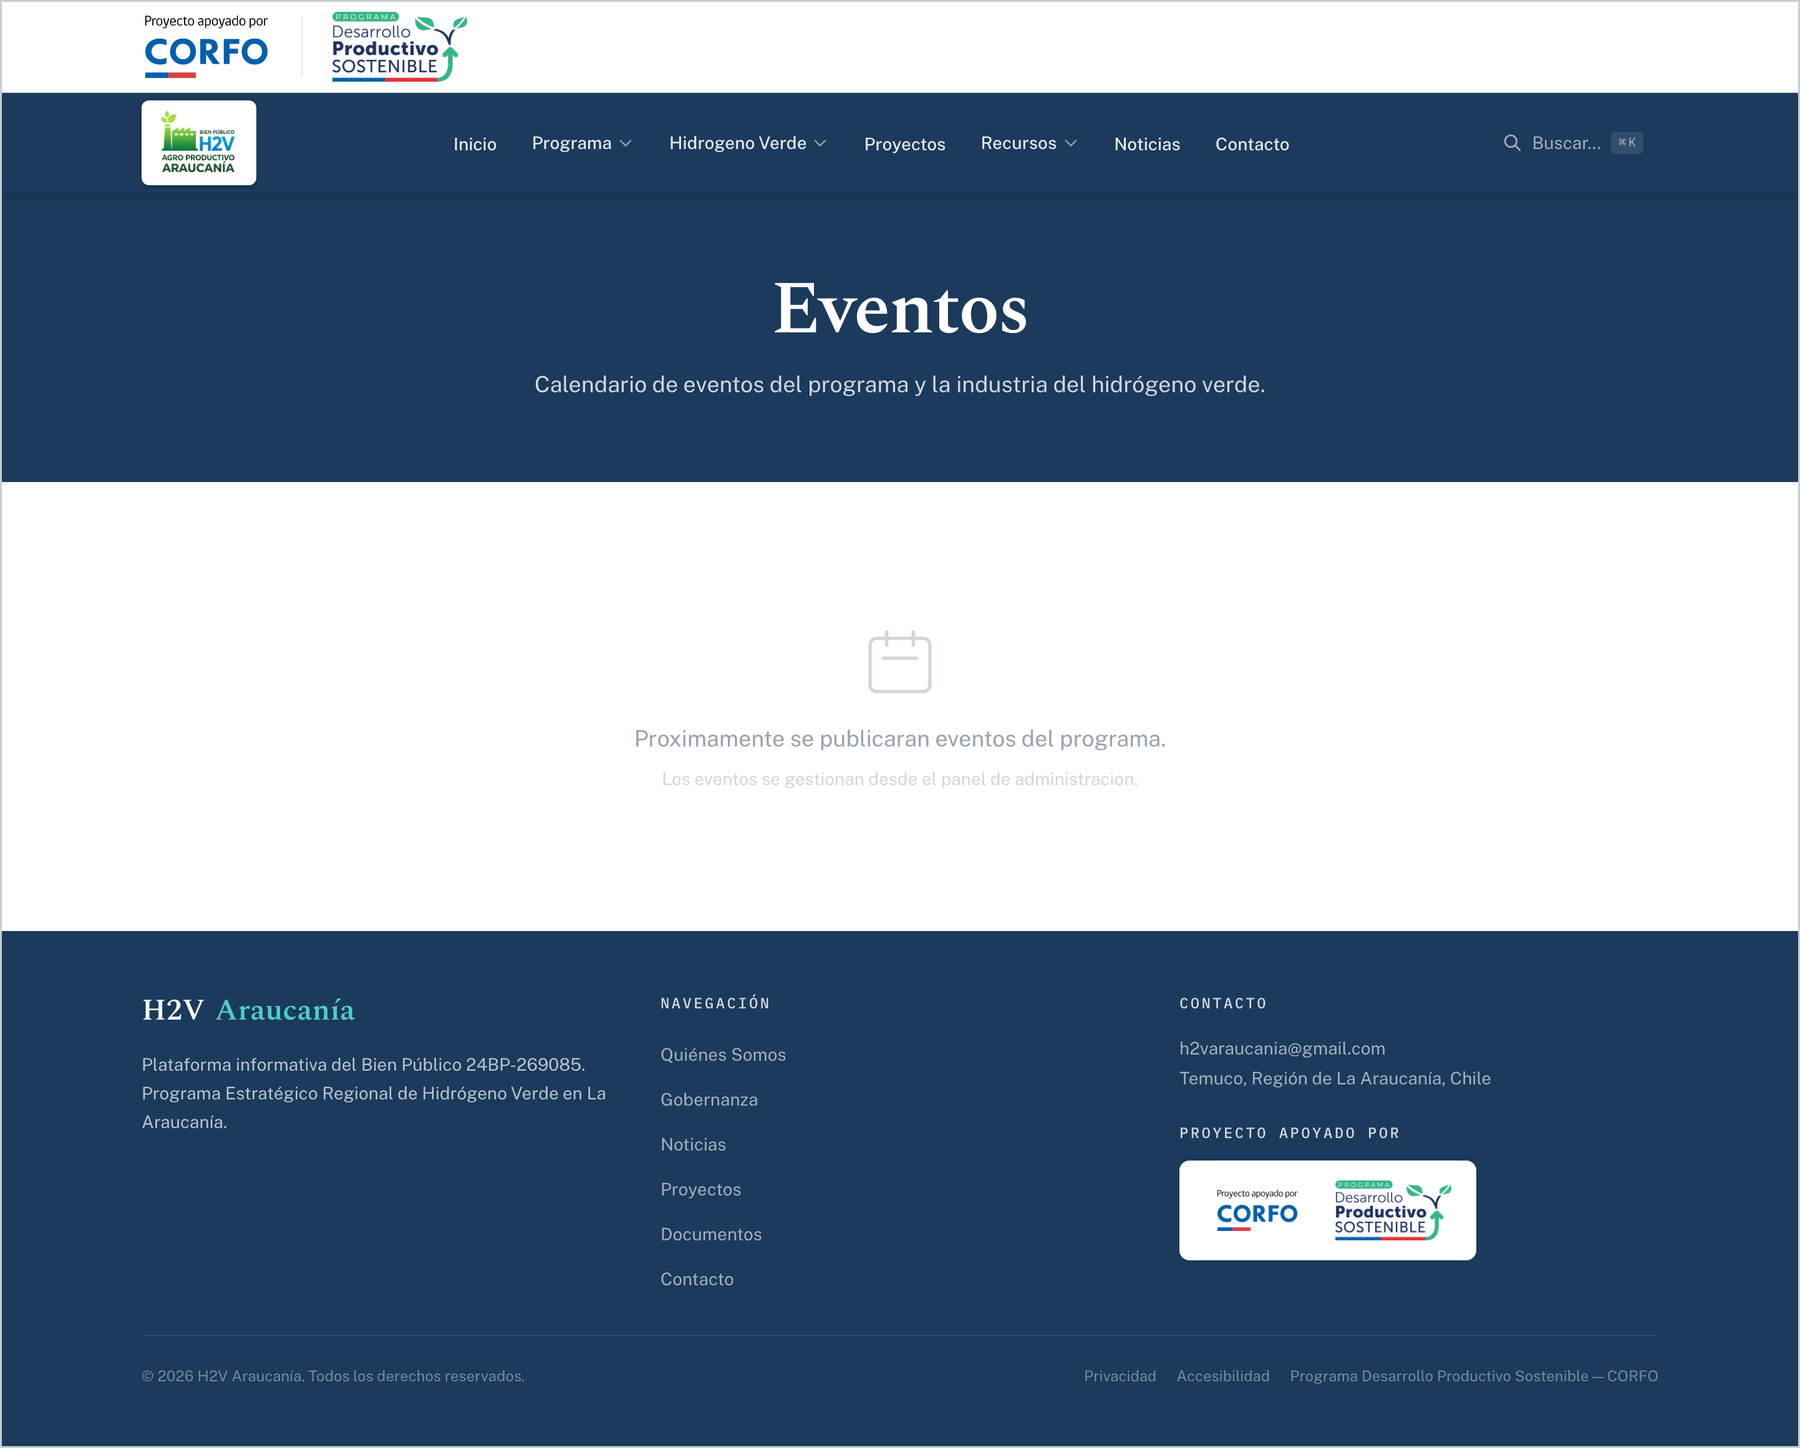
\includegraphics[width=\linewidth,keepaspectratio]{48-web-eventos.png}
\caption{Así se ve la sección Eventos del sitio público.}
\end{figure}
\section{Subir un documento}
Los documentos aparecen en \textbf{Recursos $\rightarrow$ Documentos} del sitio, con filtros por tipo y año. Los visitantes registrados pueden descargarlos y cada descarga queda contada.

\begin{enumerate}
  \item Menú lateral $\rightarrow$ \textbf{Documentos} $\rightarrow$ \textbf{Crear nuevo}.
  \item Complete:
\end{enumerate}
\begin{longtable}{>{\raggedright\arraybackslash}p{0.229\textwidth}>{\raggedright\arraybackslash}p{0.546\textwidth}>{\raggedright\arraybackslash}p{0.155\textwidth}}
\rowcolor{h2vazul}\textbf{\color{white}Campo} & \textbf{\color{white}Qué escribir} & \textbf{\color{white}Obligatorio} \\
\endfirsthead
\rowcolor{h2vazul}\textbf{\color{white}Campo} & \textbf{\color{white}Qué escribir} & \textbf{\color{white}Obligatorio} \\
\endhead
\textbf{Título del documento} & Nombre descriptivo. Máximo 120 caracteres. & Sí \\ \midrule
\rowcolor{filaalt}\textbf{Descripción} & Dos o tres oraciones sobre el contenido. Máximo 400 caracteres (se muestra completa en la tarjeta del sitio). & Sí \\ \midrule
\textbf{Archivo para descargar} & El PDF o Word que los visitantes descargarán. & Sí \\ \midrule
\rowcolor{filaalt}\textbf{Imagen de portada} & Miniatura del documento (por ejemplo, la portada del PDF como imagen). Si no sube una, se muestra un icono genérico. & No \\ \midrule
\textbf{Tipo de documento} (barra lateral) & Técnico, Difusión, Regulatorio o Capacitación. & Sí \\ \midrule
\rowcolor{filaalt}\textbf{Año} (barra lateral) & Año del documento. & Sí \\ \midrule
\textbf{Descargas} (barra lateral) & Contador automático. \textbf{No lo modifique.} & Automático \\ \bottomrule
\end{longtable}
\begin{enumerate}[start=3]
  \item Pulse \textbf{Guardar}. El documento queda visible de inmediato.
\end{enumerate}
\begin{figure}[H]\centering
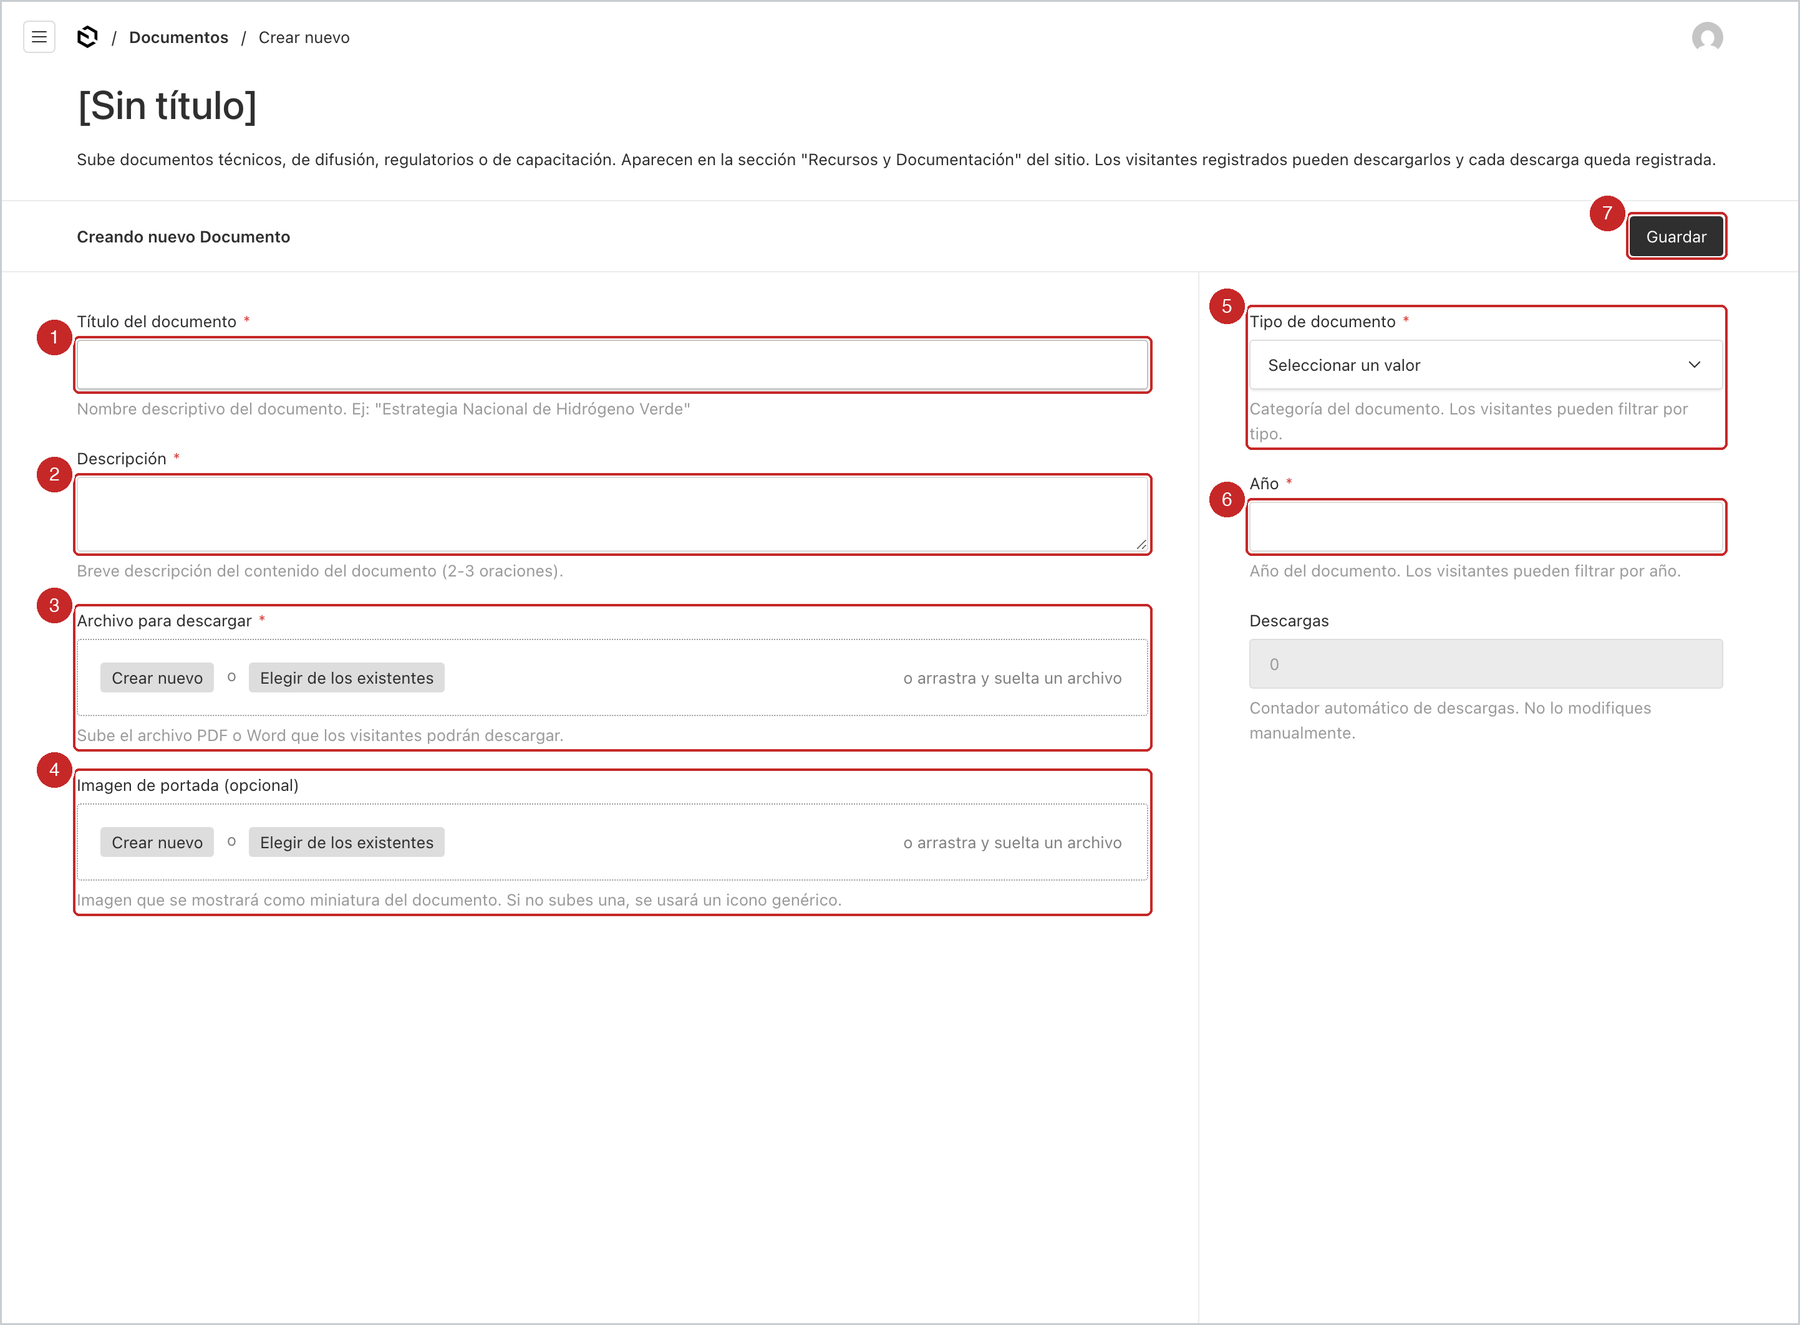
\includegraphics[width=\linewidth,keepaspectratio]{12-documento-crear.png}
\caption{Formulario de un documento nuevo: título (1), descripción (2), archivo (3), portada (4), tipo (5), año (6) y Guardar (7).}
\end{figure}
\begin{figure}[H]\centering
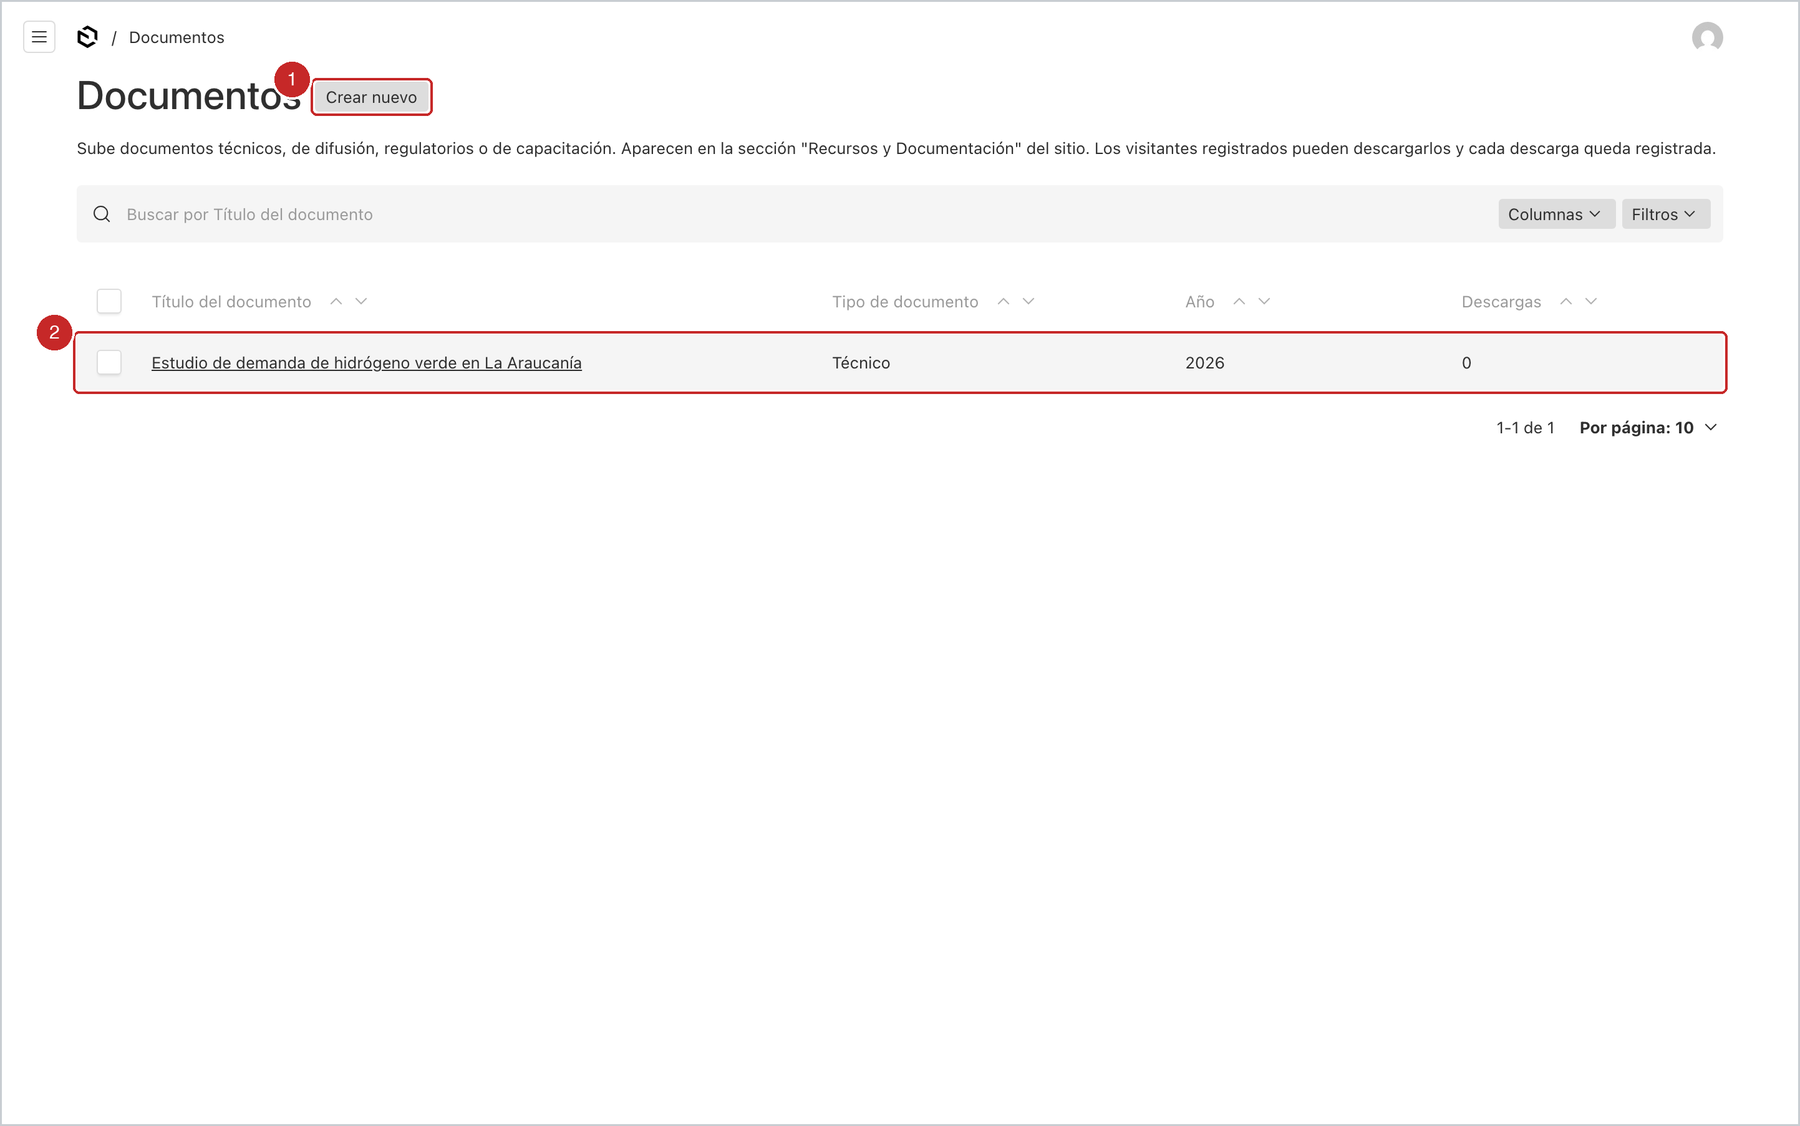
\includegraphics[width=\linewidth,keepaspectratio]{12b-documentos-lista.png}
\caption{Lista de documentos en el panel: Crear nuevo (1) y filas existentes (2).}
\end{figure}
\begin{figure}[H]\centering
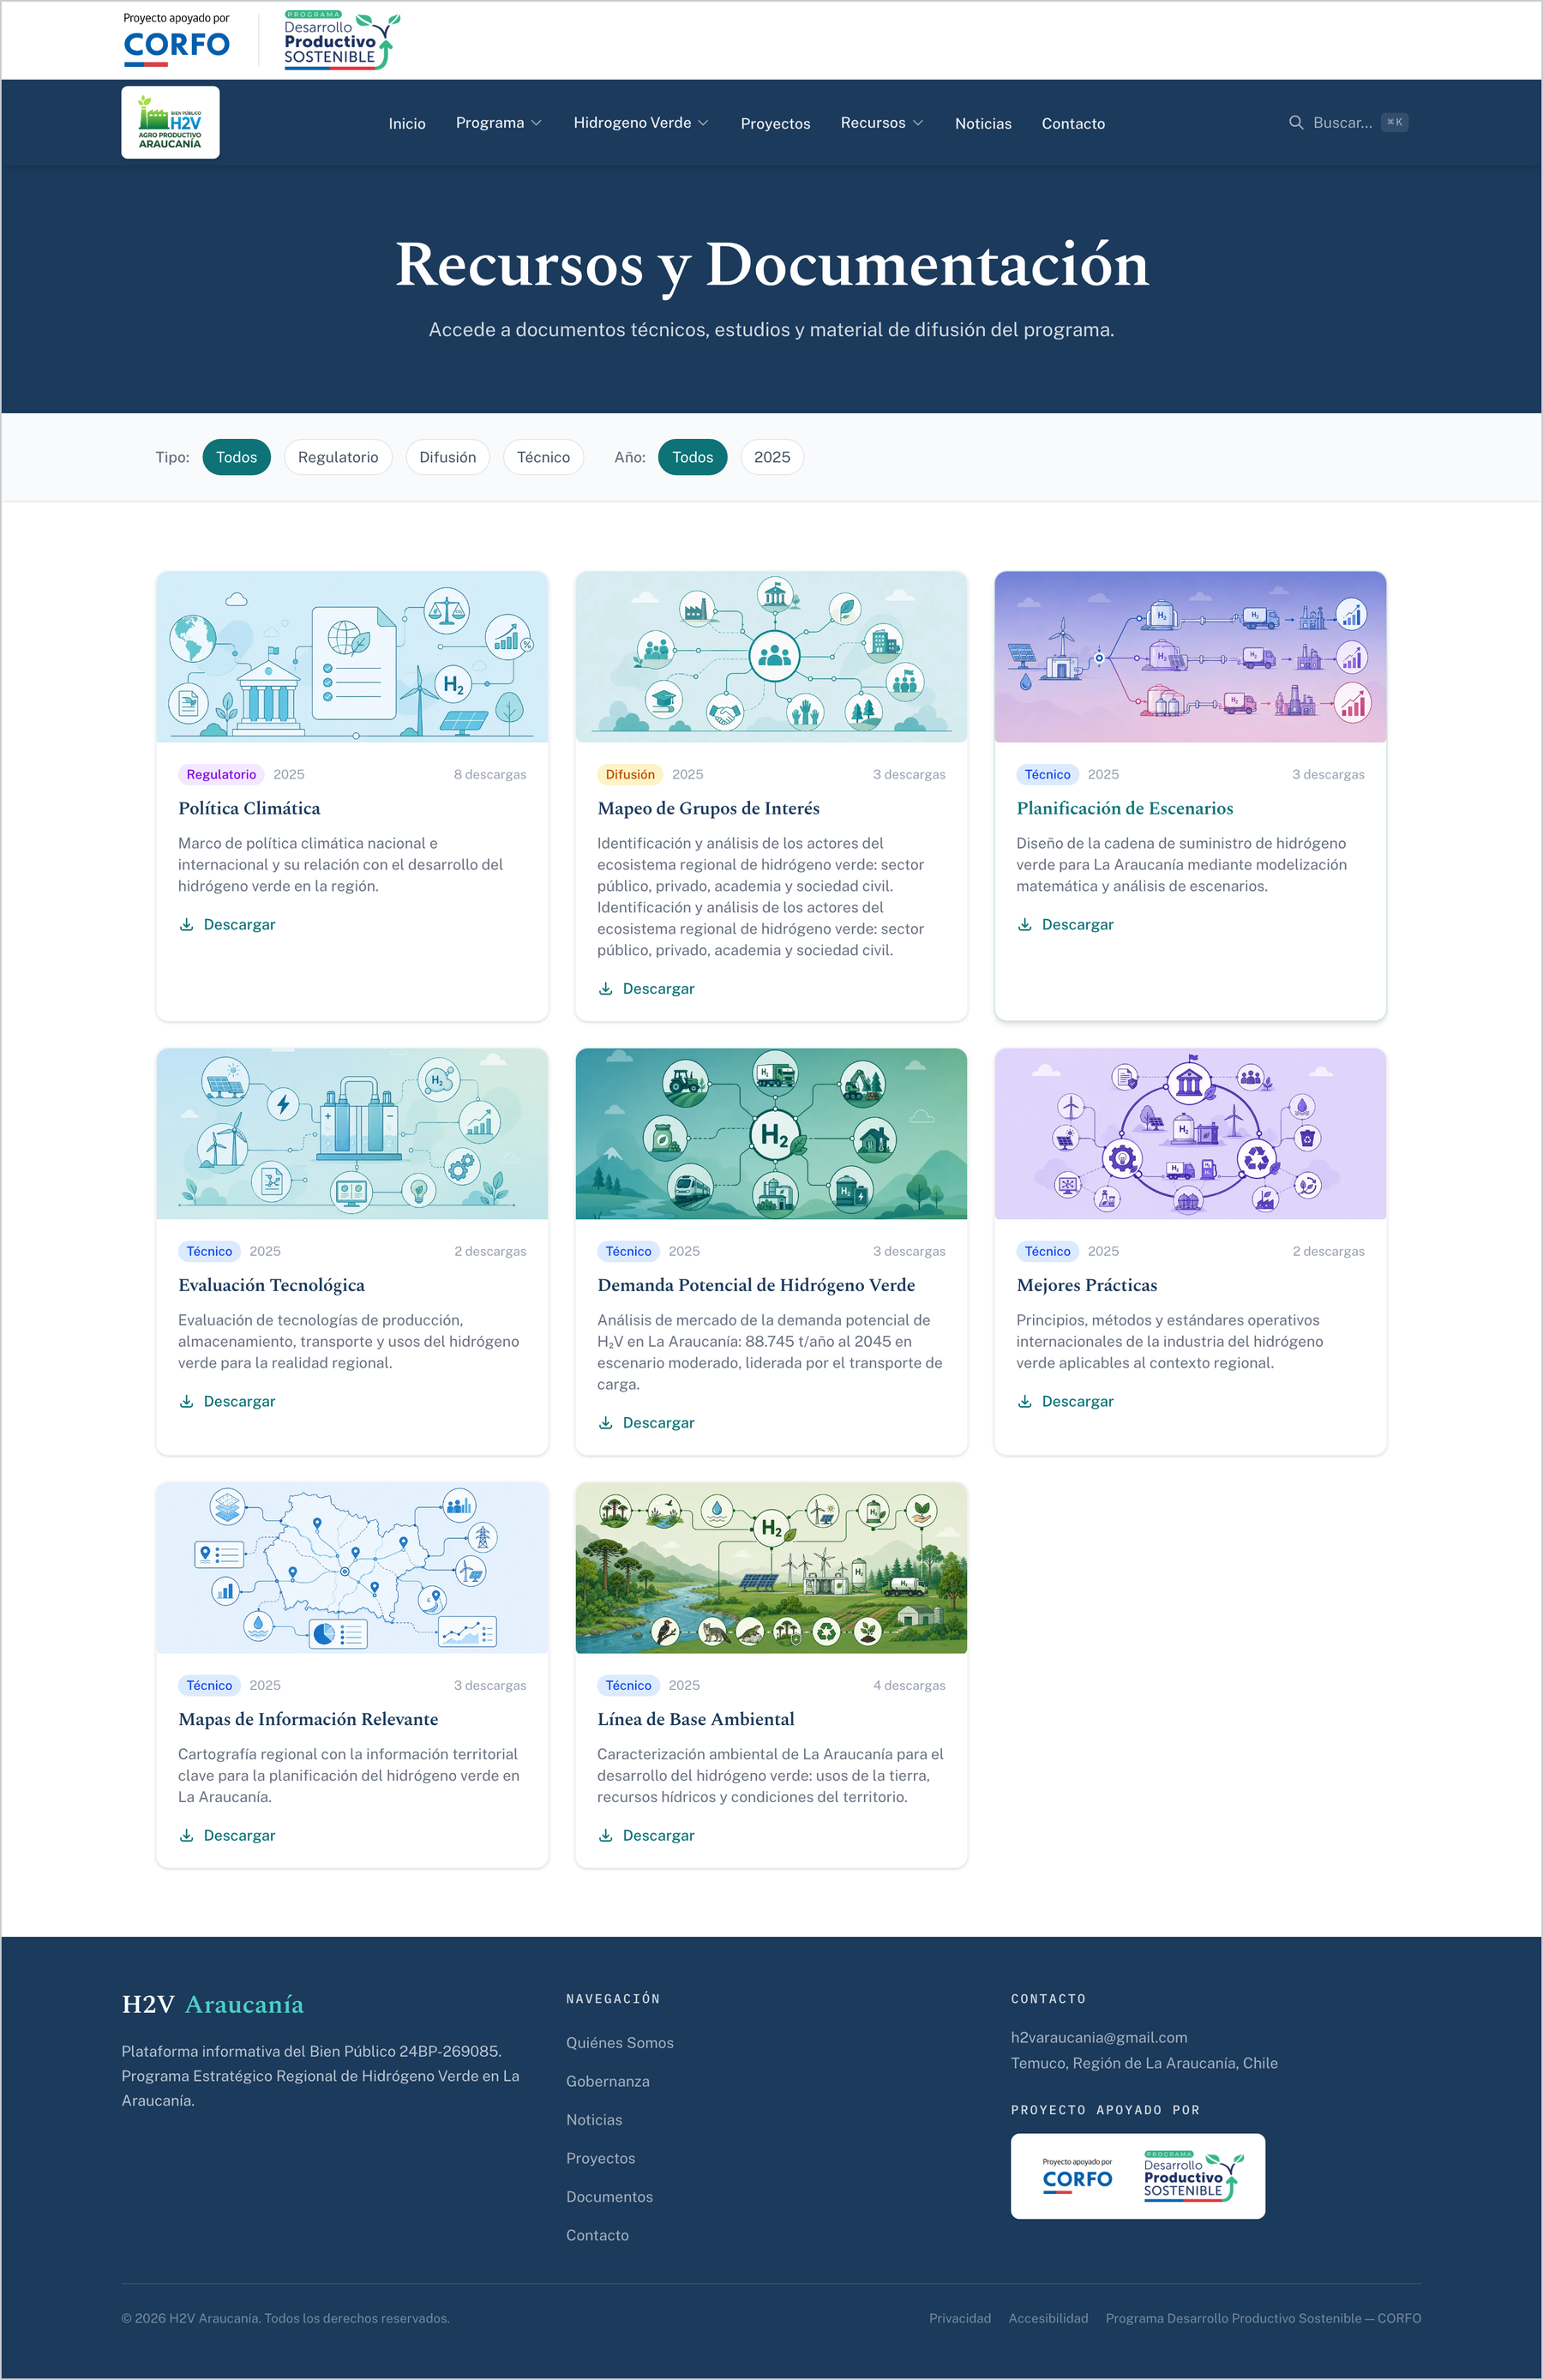
\includegraphics[width=\linewidth,height=0.74\textheight,keepaspectratio]{45-web-documentos.png}
\caption{Así se ve la sección Recursos y Documentación del sitio público.}
\end{figure}
\section{Agregar un proyecto al mapa}
El \textbf{Mapa de Proyectos} del sitio muestra un punto por cada proyecto de hidrógeno verde, con un globo de información al hacer clic.

\begin{enumerate}
  \item Menú lateral $\rightarrow$ \textbf{Proyectos} $\rightarrow$ \textbf{Crear nuevo}.
  \item Complete:
\end{enumerate}
\begin{longtable}{>{\raggedright\arraybackslash}p{0.271\textwidth}>{\raggedright\arraybackslash}p{0.505\textwidth}>{\raggedright\arraybackslash}p{0.155\textwidth}}
\rowcolor{h2vazul}\textbf{\color{white}Campo} & \textbf{\color{white}Qué escribir} & \textbf{\color{white}Obligatorio} \\
\endfirsthead
\rowcolor{h2vazul}\textbf{\color{white}Campo} & \textbf{\color{white}Qué escribir} & \textbf{\color{white}Obligatorio} \\
\endhead
\textbf{Nombre del proyecto} & Ejemplo: ''Planta piloto H2V Temuco''. Máximo 100 caracteres. & Sí \\ \midrule
\rowcolor{filaalt}\textbf{Descripción} & Dos a cuatro oraciones; aparece en el globo del mapa. Máximo 400 caracteres. & Sí \\ \midrule
\textbf{Empresa o entidad} & Responsable del proyecto. Máximo 80 caracteres. & Sí \\ \midrule
\rowcolor{filaalt}\textbf{Coordenadas geográficas: Latitud y Longitud} & La ubicación del punto (vea cómo obtenerlas más abajo). & Sí \\ \midrule
\textbf{Etapa actual} (barra lateral) & Planificación, Pilotaje, Desarrollo u Operación (cambia el color del punto). & Sí \\ \midrule
\rowcolor{filaalt}\textbf{Ubicación} (barra lateral) & Araucanía o Nacional (otra región). & Sí \\ \midrule
\textbf{Capacidad (MW)} y \textbf{Producción (ton/año)} (barra lateral) & Si se conocen. & No \\ \midrule
\rowcolor{filaalt}\textbf{Imagen del proyecto} & Foto o render; aparece en el globo del mapa. & No \\ \midrule
\textbf{Enlace externo} & Dirección web del proyecto o empresa (con \url{https://}); aparece como ''Ver sitio del proyecto''. & No \\ \bottomrule
\end{longtable}
\begin{enumerate}[start=3]
  \item Pulse \textbf{Guardar}.
\end{enumerate}
\begin{figure}[H]\centering
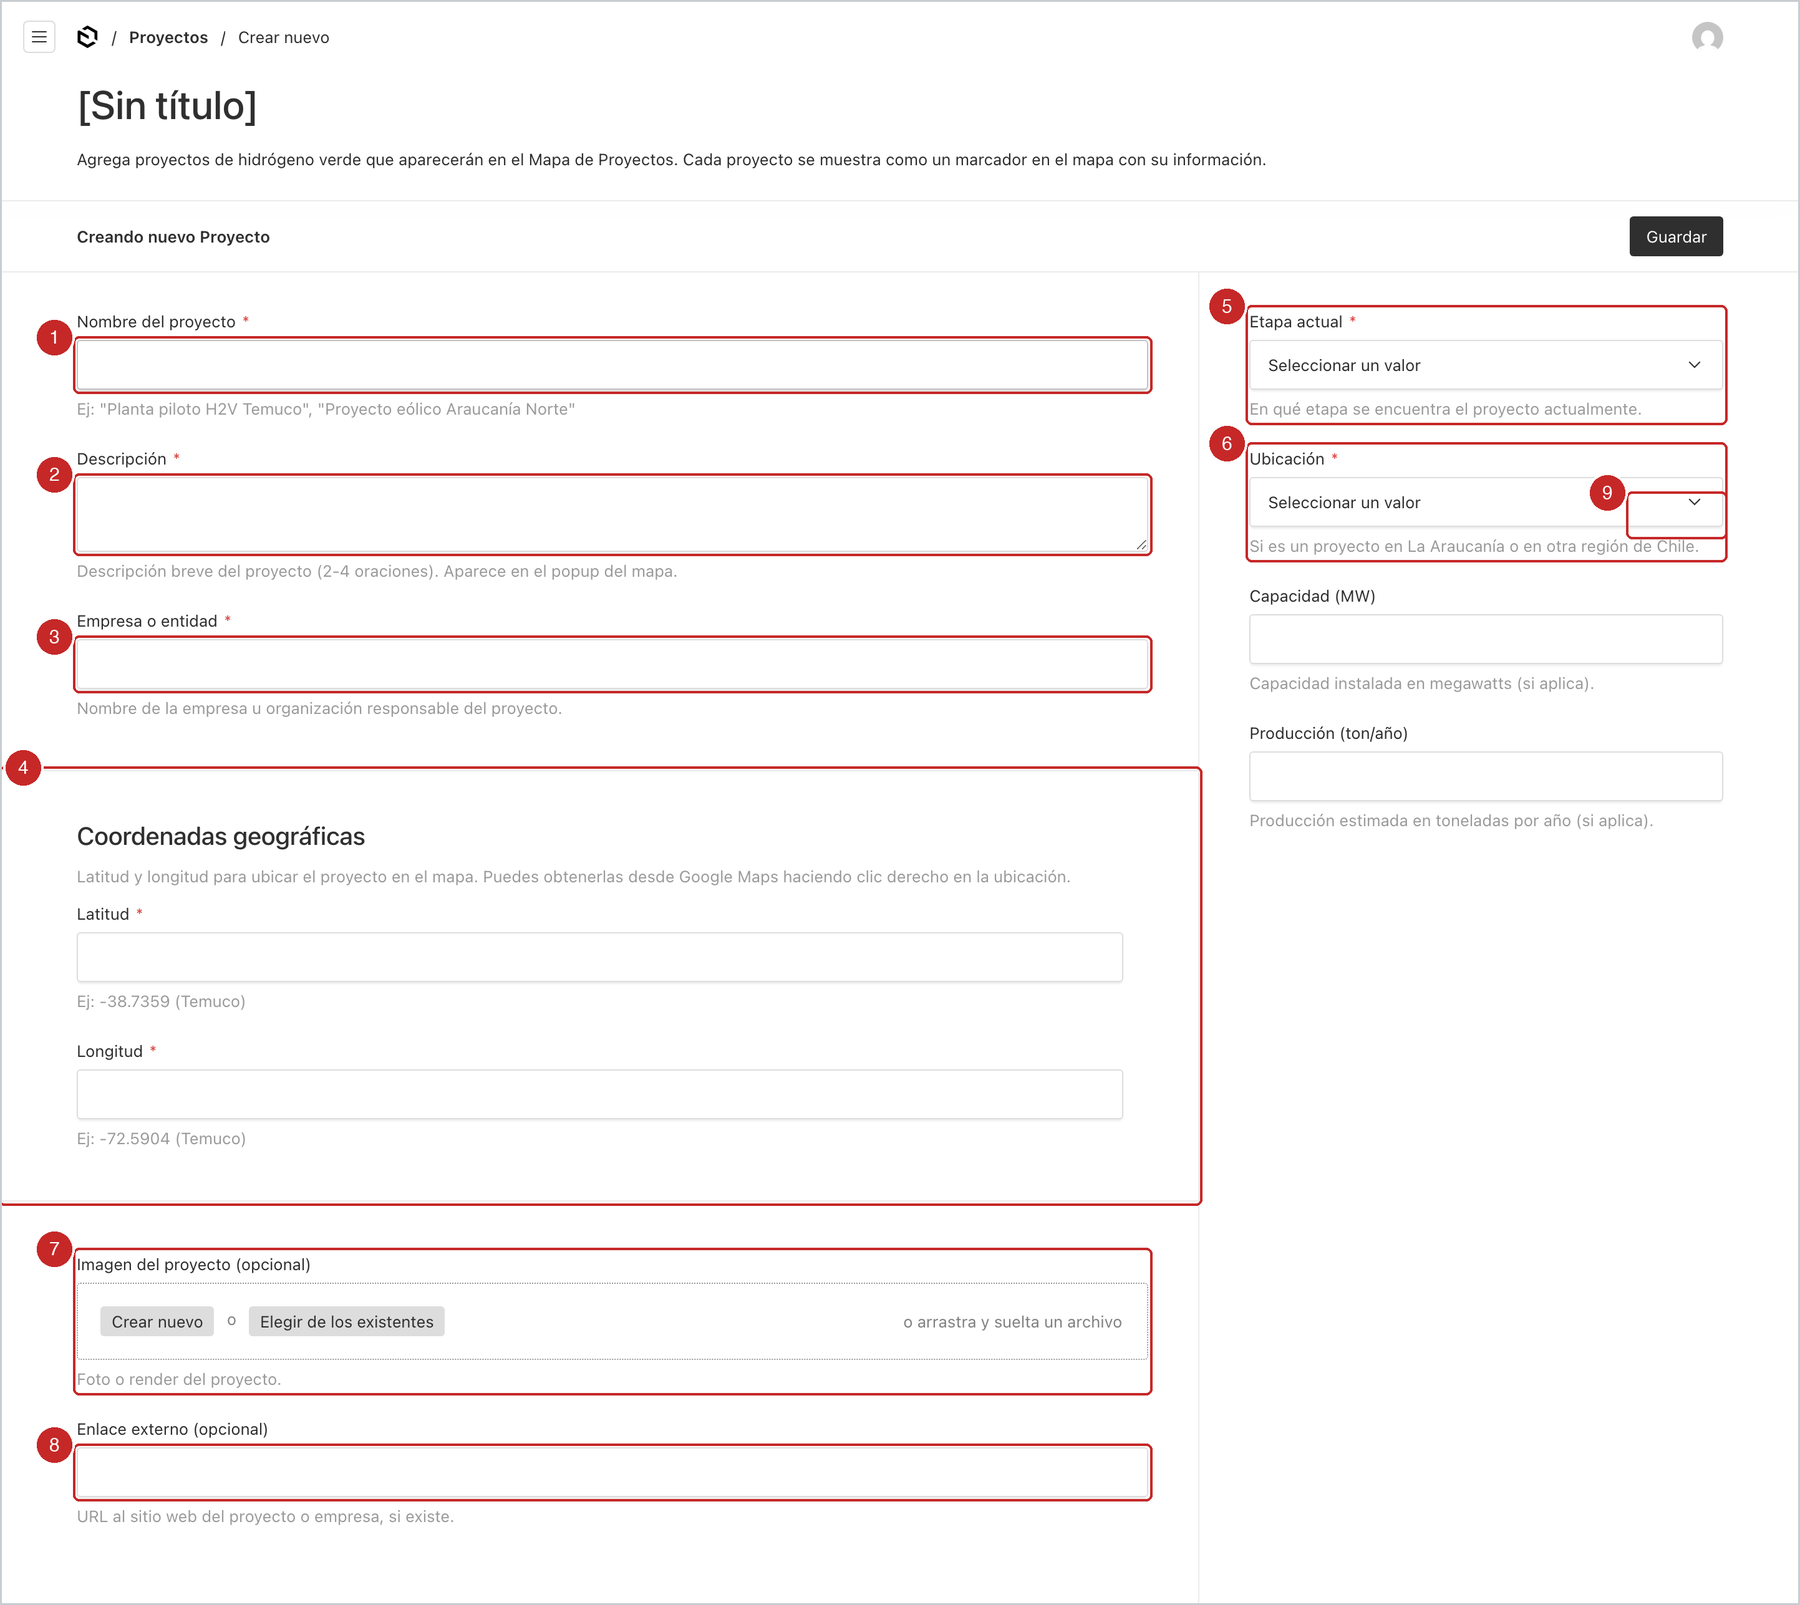
\includegraphics[width=\linewidth,keepaspectratio]{13-proyecto-crear.png}
\caption{Formulario de un proyecto nuevo: nombre (1), descripción (2), empresa (3), coordenadas (4), etapa (5), ubicación (6), imagen (7), enlace (8) y Guardar (9).}
\end{figure}
\textbf{Cómo obtener las coordenadas con Google Maps:}

\begin{enumerate}
  \item Abra \url{maps.google.com} y busque el lugar del proyecto.
  \item Haga \textbf{clic derecho} sobre el punto exacto del mapa.
  \item El primer renglón del menú muestra dos números, por ejemplo \texttt{-38.7359, -72.5904}. Haga clic sobre ellos para copiarlos.
  \item El primer número es la \textbf{Latitud} y el segundo la \textbf{Longitud}. Péguelos en los campos correspondientes.
\end{enumerate}
\begin{recuadro}{cAtencion}{bAtencion}\textbf{\color{bAtencion}Atención:} en Chile la latitud y la longitud son siempre números \textbf{negativos} (latitud entre -17 y -56; longitud entre -66 y -76). Si el punto aparece en el mar o en otro país, lo más probable es que haya invertido latitud y longitud.\end{recuadro}
\begin{figure}[H]\centering
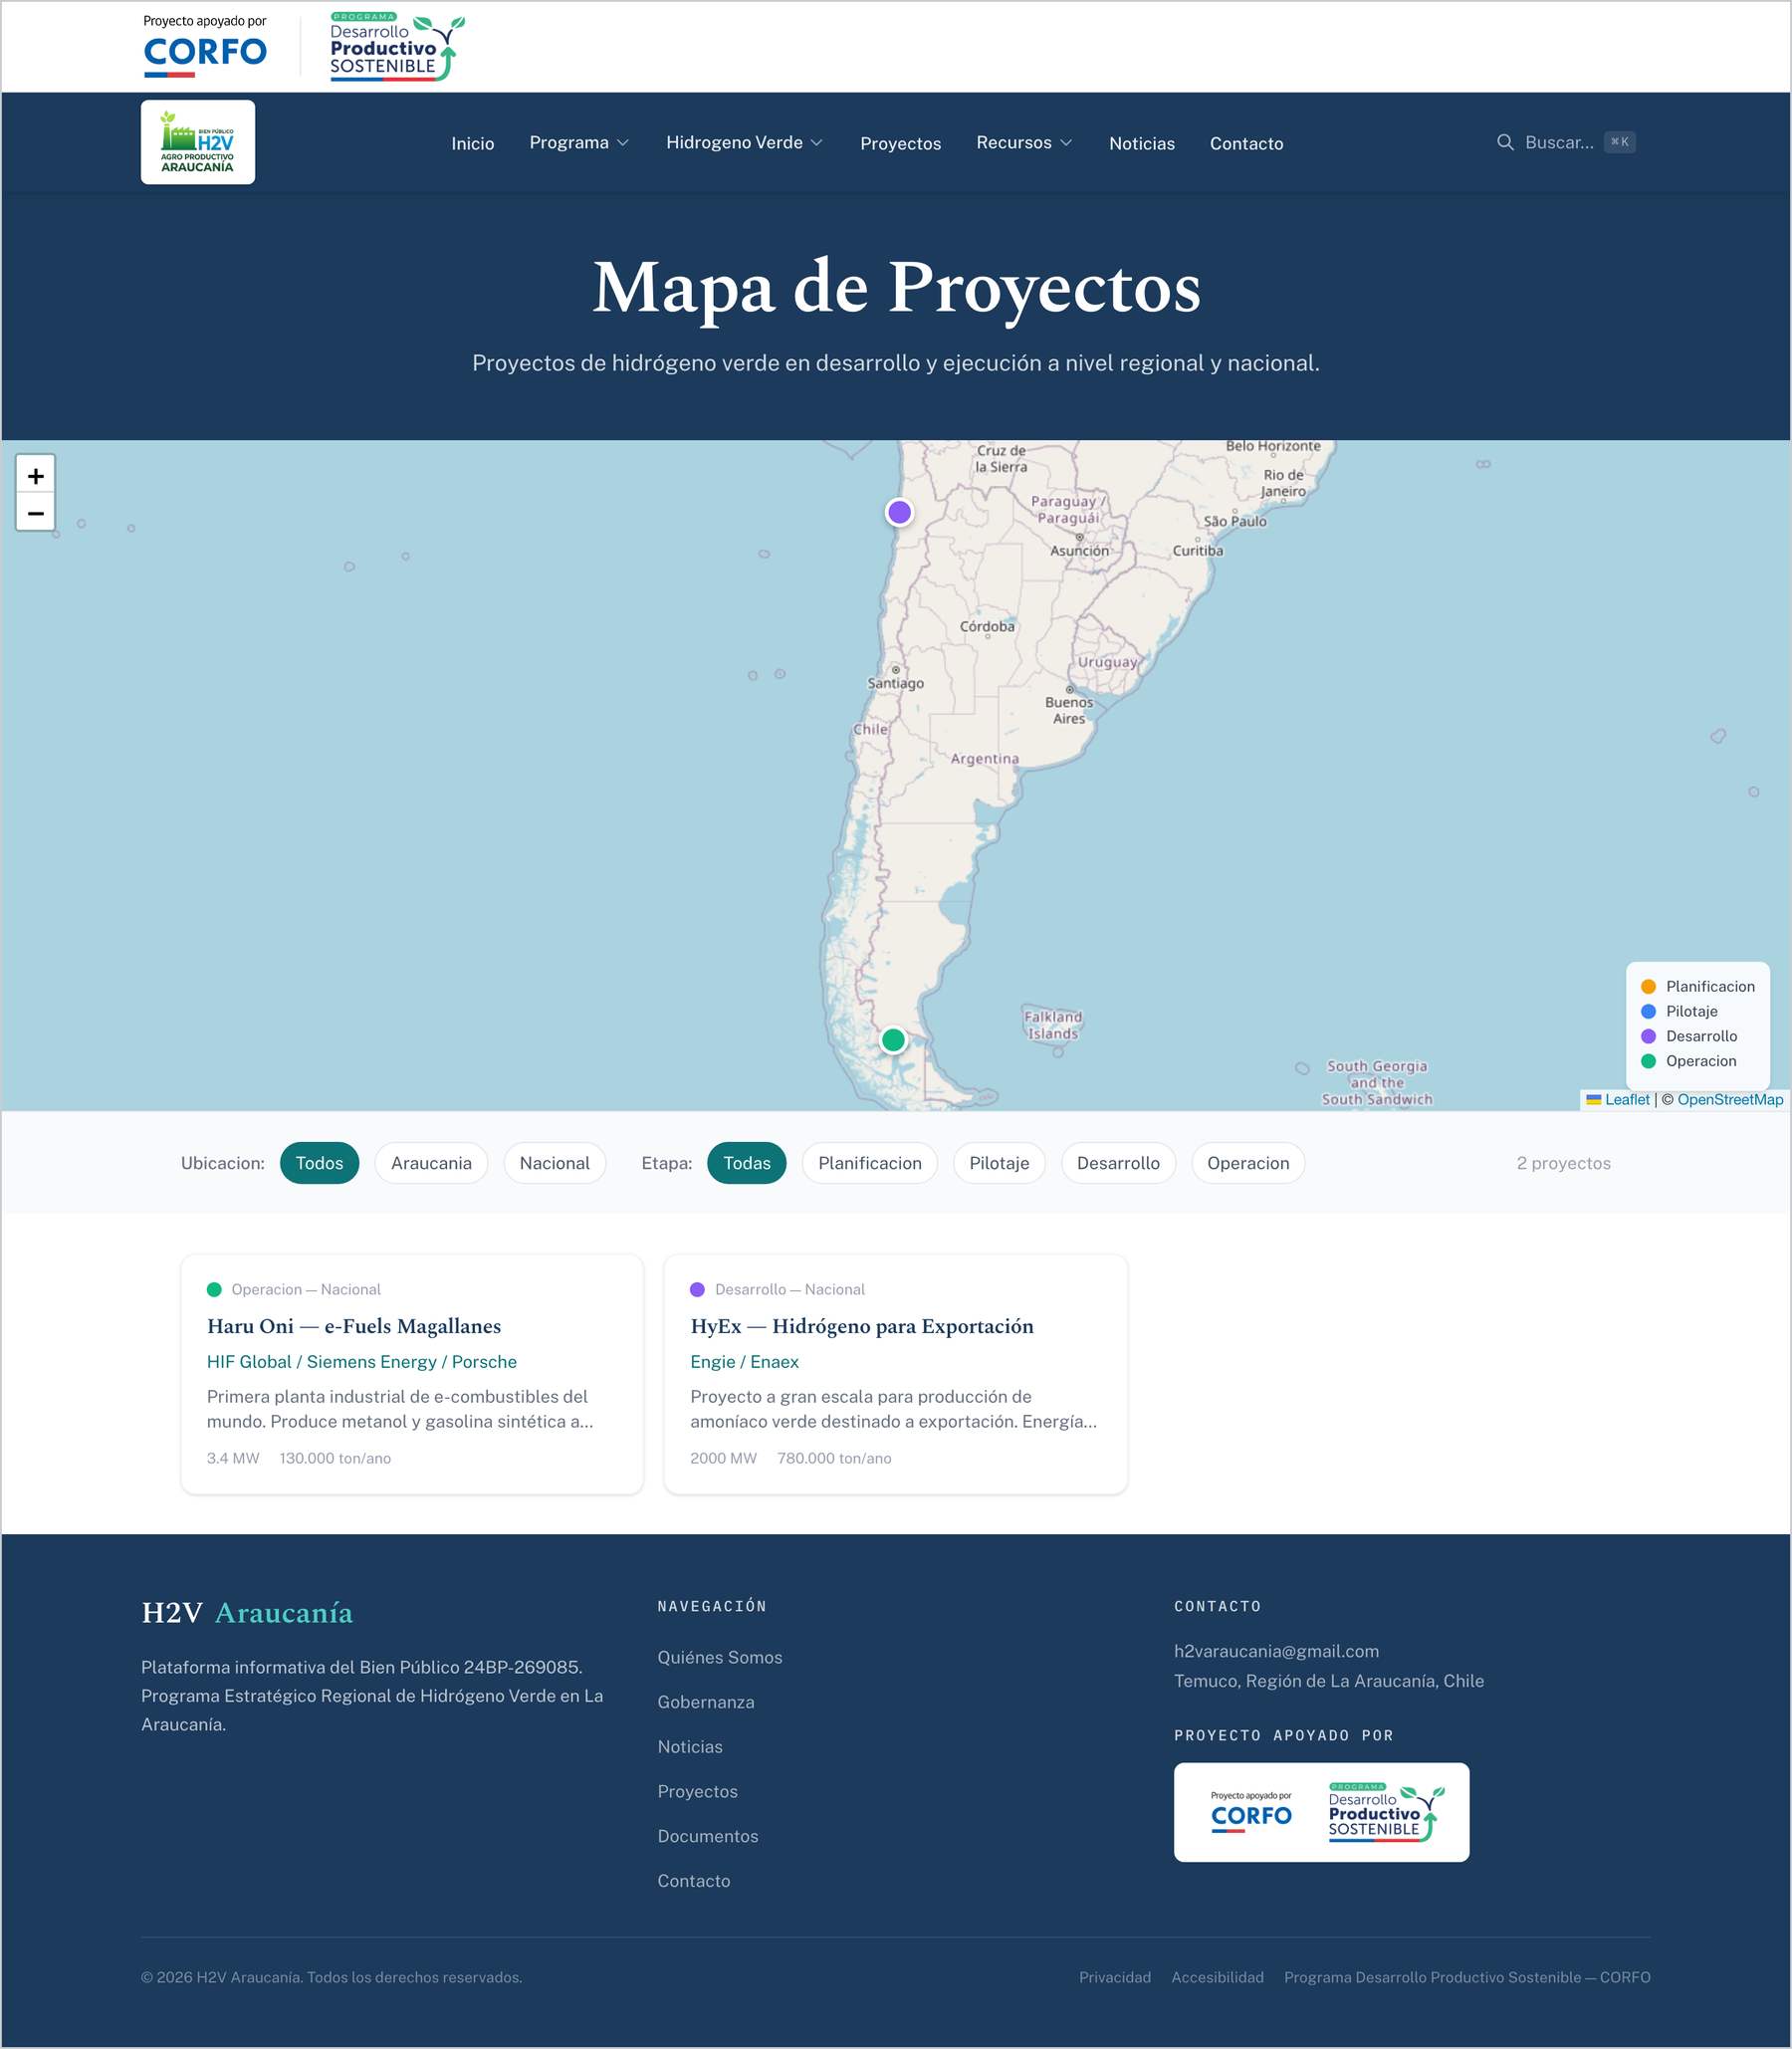
\includegraphics[width=\linewidth,keepaspectratio]{46-web-proyectos.png}
\caption{Así se ve el Mapa de Proyectos del sitio público.}
\end{figure}
\section{Dibujar la forma de un proyecto en el mapa (archivos KMZ)}
Cada proyecto aparece en el mapa como un \textbf{círculo de color}, en el lugar de sus coordenadas. Además, puede mostrar la \textbf{forma real de su terreno} (el contorno del predio) o de una obra (el trazado de un ducto o de un camino). Esa forma se dibuja en \textbf{Google Earth} y se sube al sitio como un archivo \textbf{KMZ} o \textbf{KML}.

\begin{recuadro}{cNota}{bNota}\textbf{\color{bNota}Nota:} un archivo KMZ o KML es el archivo en que Google Earth guarda un dibujo hecho sobre el mapa: puntos, líneas o formas, con sus coordenadas. Son lo mismo: el KMZ es la versión comprimida del KML. El sitio acepta los dos.\end{recuadro}
\textbf{Qué se ve en el mapa:}

\begin{longtable}{>{\raggedright\arraybackslash}p{0.149\textwidth}>{\raggedright\arraybackslash}p{0.352\textwidth}>{\raggedright\arraybackslash}p{0.428\textwidth}}
\rowcolor{h2vazul}\textbf{\color{white}Lo que ve} & \textbf{\color{white}Qué significa} & \textbf{\color{white}De dónde sale} \\
\endfirsthead
\rowcolor{h2vazul}\textbf{\color{white}Lo que ve} & \textbf{\color{white}Qué significa} & \textbf{\color{white}De dónde sale} \\
\endhead
\textbf{Un círculo} & Dónde está el proyecto. Al hacerle clic se abre su ficha. & De la Latitud y Longitud escritas en el formulario del proyecto. Todo proyecto lo tiene, con o sin archivo KMZ. \\ \midrule
\rowcolor{filaalt}\textbf{Una forma} (polígono o línea) & Qué superficie ocupa el proyecto, o por dónde pasa una obra. & Del archivo KMZ unido al proyecto. \\ \bottomrule
\end{longtable}
Los dos se pintan con el \textbf{color de la etapa} del proyecto: anaranjado para Planificación, azul para Pilotaje, morado para Desarrollo y verde para Operación.

El trabajo tiene cuatro partes: \textbf{dibujar} la forma en Google Earth, \textbf{subir} el archivo al panel, \textbf{unirlo} al proyecto y \textbf{comprobar} el resultado en el sitio.

\subsection{Parte 1. Dibujar la forma en Google Earth}
Se usa Google Earth en el navegador: es gratis, no hay que instalar nada y el archivo queda guardado en su computador.

\begin{enumerate}
  \item Abra \textbf{earth.google.com} en Chrome. Si se lo pide, entre con cualquier cuenta de Google.
  \item Arriba a la izquierda, abra el menú \textbf{Archivo} y elija \textbf{Nuevo archivo KML local}. Otra forma de llegar: en la pantalla de inicio, botón \textbf{Editor de KML local} $\rightarrow$ \textbf{Crear un nuevo archivo KML}.
  \item Escriba el lugar del proyecto en el buscador de arriba (\textbf{Buscar en Google Earth}) y acérquese hasta ver bien el terreno.
  \item Abra el menú \textbf{Agregar} $\rightarrow$ \textbf{Línea o forma} $\rightarrow$ \textbf{Ruta o polígono}.
  \item Haga clic en cada esquina del terreno, una tras otra. Para cerrar la forma, haga clic otra vez sobre \textbf{el primer punto}. Si lo que dibuja es una línea (por ejemplo, un ducto), termínela con doble clic.
  \item Haga clic en \textbf{Listo} y luego en \textbf{Guardar en el proyecto}. Si le pide un nombre, escriba uno claro, por ejemplo ''Predio planta Temuco''.
  \item Abra el menú \textbf{Archivo} y elija \textbf{Exportar como archivo KML}. El archivo queda en la carpeta \textbf{Descargas} de su computador.
\end{enumerate}
\begin{recuadro}{cConsejo}{bConsejo}\textbf{\color{bConsejo}Consejo:} si la empresa o alguien del equipo ya le envió el archivo KMZ o KML del proyecto, no necesita dibujar nada: pase directo a la Parte 2. Si usa el programa \textbf{Google Earth Pro} (el que se instala), el archivo se obtiene con clic derecho sobre lo dibujado $\rightarrow$ \textbf{Guardar lugar como...} $\rightarrow$ formato KMZ.\end{recuadro}
\begin{recuadro}{cAtencion}{bAtencion}\textbf{\color{bAtencion}Atención:} Google Earth cambia sus pantallas de vez en cuando. Si un botón aparece con un nombre algo distinto (por ejemplo ''Terminar'' en vez de ''Listo''), use el equivalente.\end{recuadro}
\subsection{Parte 2. Subir el archivo al panel}
\begin{enumerate}
  \item Entre al panel. En el menú de la izquierda, grupo \textbf{Contenido}, haga clic en \textbf{Capas geográficas (KMZ)}.
  \item Arriba, haga clic en \textbf{Crear nuevo}.
  \item Complete el formulario:
\end{enumerate}
\begin{longtable}{>{\raggedright\arraybackslash}p{0.155\textwidth}>{\raggedright\arraybackslash}p{0.629\textwidth}>{\raggedright\arraybackslash}p{0.155\textwidth}}
\rowcolor{h2vazul}\textbf{\color{white}Campo} & \textbf{\color{white}Qué poner} & \textbf{\color{white}Obligatorio} \\
\endfirsthead
\rowcolor{h2vazul}\textbf{\color{white}Campo} & \textbf{\color{white}Qué poner} & \textbf{\color{white}Obligatorio} \\
\endhead
\textbf{Título de la capa} & Un nombre claro. Ejemplo: ''Predio planta Temuco''. & Sí \\ \midrule
\rowcolor{filaalt}\textbf{Tipo de capa} & \textbf{Geometría de un proyecto}, que es el caso normal. El otro tipo se explica al final de esta sección. & Sí \\ \midrule
\textbf{El archivo} & Arrastre el archivo .kmz o .kml a la zona gris, o haga clic ahí y búsquelo en su carpeta Descargas. & Sí \\ \midrule
\rowcolor{filaalt}\textbf{Descripción} & Una frase sobre qué muestra la capa. & No \\ \midrule
\textbf{Color} (columna derecha) & Déjelo vacío para usar el color de la etapa del proyecto. Solo si quiere otro color, escriba su código, por ejemplo \texttt{\#0D7377}. & No \\ \bottomrule
\end{longtable}
\begin{enumerate}[start=4]
  \item Haga clic en \textbf{Guardar}.
  \item Revise el resultado. En unos segundos el formulario muestra lo que el sistema encontró en el archivo: \textbf{Resultado del procesamiento} debe decir \textbf{''Sin observaciones.''} y \textbf{N.º de geometrías} indica cuántas formas encontró.
\end{enumerate}
\begin{figure}[H]\centering
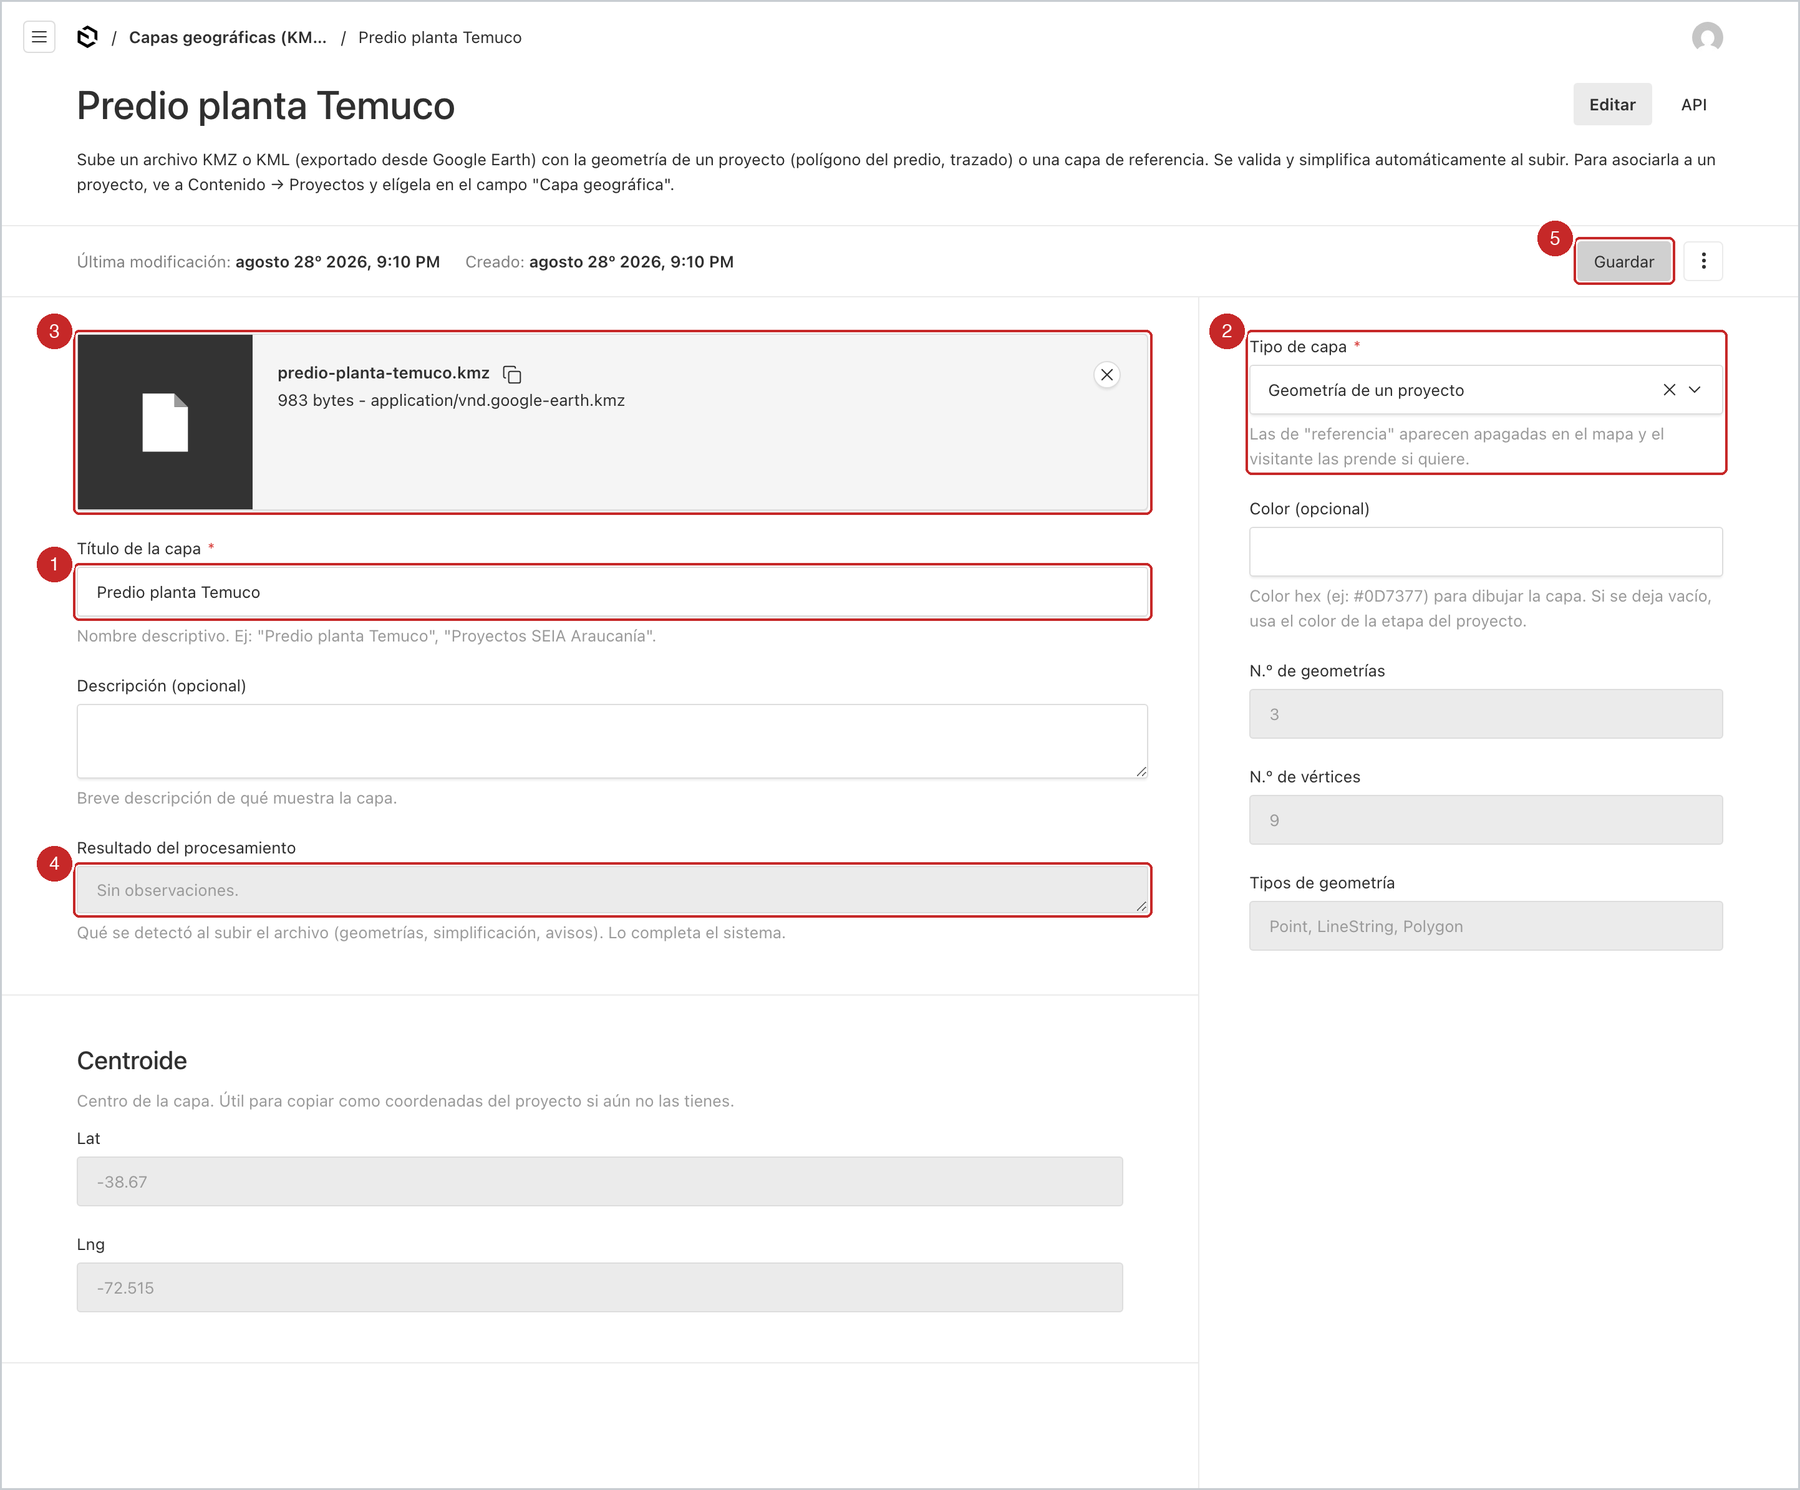
\includegraphics[width=\linewidth,keepaspectratio]{13b-capa-kmz.png}
\caption{La capa ya guardada: título (1), tipo (2), el archivo subido (3), el resultado del procesamiento, que completa el sistema (4), y Guardar (5).}
\end{figure}
\begin{recuadro}{cResultado}{bResultado}\textbf{\color{bResultado}Resultado:} la capa queda guardada. Todavía no se ve en el sitio: falta unirla a un proyecto (Parte 3).\end{recuadro}
Si el archivo tiene un problema, el panel muestra un mensaje rojo y \textbf{no lo guarda}. Estos son los mensajes más comunes:

\begin{longtable}{>{\raggedright\arraybackslash}p{0.311\textwidth}>{\raggedright\arraybackslash}p{0.619\textwidth}}
\rowcolor{h2vazul}\textbf{\color{white}El mensaje dice...} & \textbf{\color{white}Qué hacer} \\
\endfirsthead
\rowcolor{h2vazul}\textbf{\color{white}El mensaje dice...} & \textbf{\color{white}Qué hacer} \\
\endhead
''El archivo supera los 4 MB permitidos'' & El archivo trae imágenes u otras capas. Exporte solo la forma del proyecto; un predio pesa unos pocos KB. \\ \midrule
\rowcolor{filaalt}''El archivo no contiene ninguna geometría'' & Se exportó sin dibujo. Vuelva a la Parte 1 y dibuje la forma antes de exportar. \\ \midrule
''Este archivo es un enlace a un mapa en línea'' & Viene de Google My Maps. Ahí use ''Exportar a KML/KMZ'' y desmarque ''Mantener los datos actualizados''. \\ \midrule
\rowcolor{filaalt}''El archivo tiene coordenadas fuera de rango'' & Probablemente la latitud y la longitud están invertidas. Vuelva a exportarlo desde Google Earth. \\ \midrule
''Se alcanzó el máximo de 50 capas'' & Elimine alguna capa que ya no se use (vea más abajo). \\ \midrule
\rowcolor{filaalt}Cualquier otro mensaje & Vuelva a exportar el archivo desde Google Earth y súbalo de nuevo. \\ \bottomrule
\end{longtable}
\subsection{Parte 3. Unir el archivo al proyecto}
\begin{enumerate}
  \item En el menú de la izquierda, grupo \textbf{Contenido}, haga clic en \textbf{Proyectos} y abra el proyecto. Si todavía no existe, créelo como se explica en ''Agregar un proyecto al mapa''.
  \item Baje hasta el final del formulario, al campo \textbf{Capa geográfica (KMZ, opcional)}.
  \item Haga clic en \textbf{Elegir de los existentes} y, en la lista que aparece, haga clic en la capa que subió.
  \item Haga clic en \textbf{Guardar}.
\end{enumerate}
\begin{figure}[H]\centering
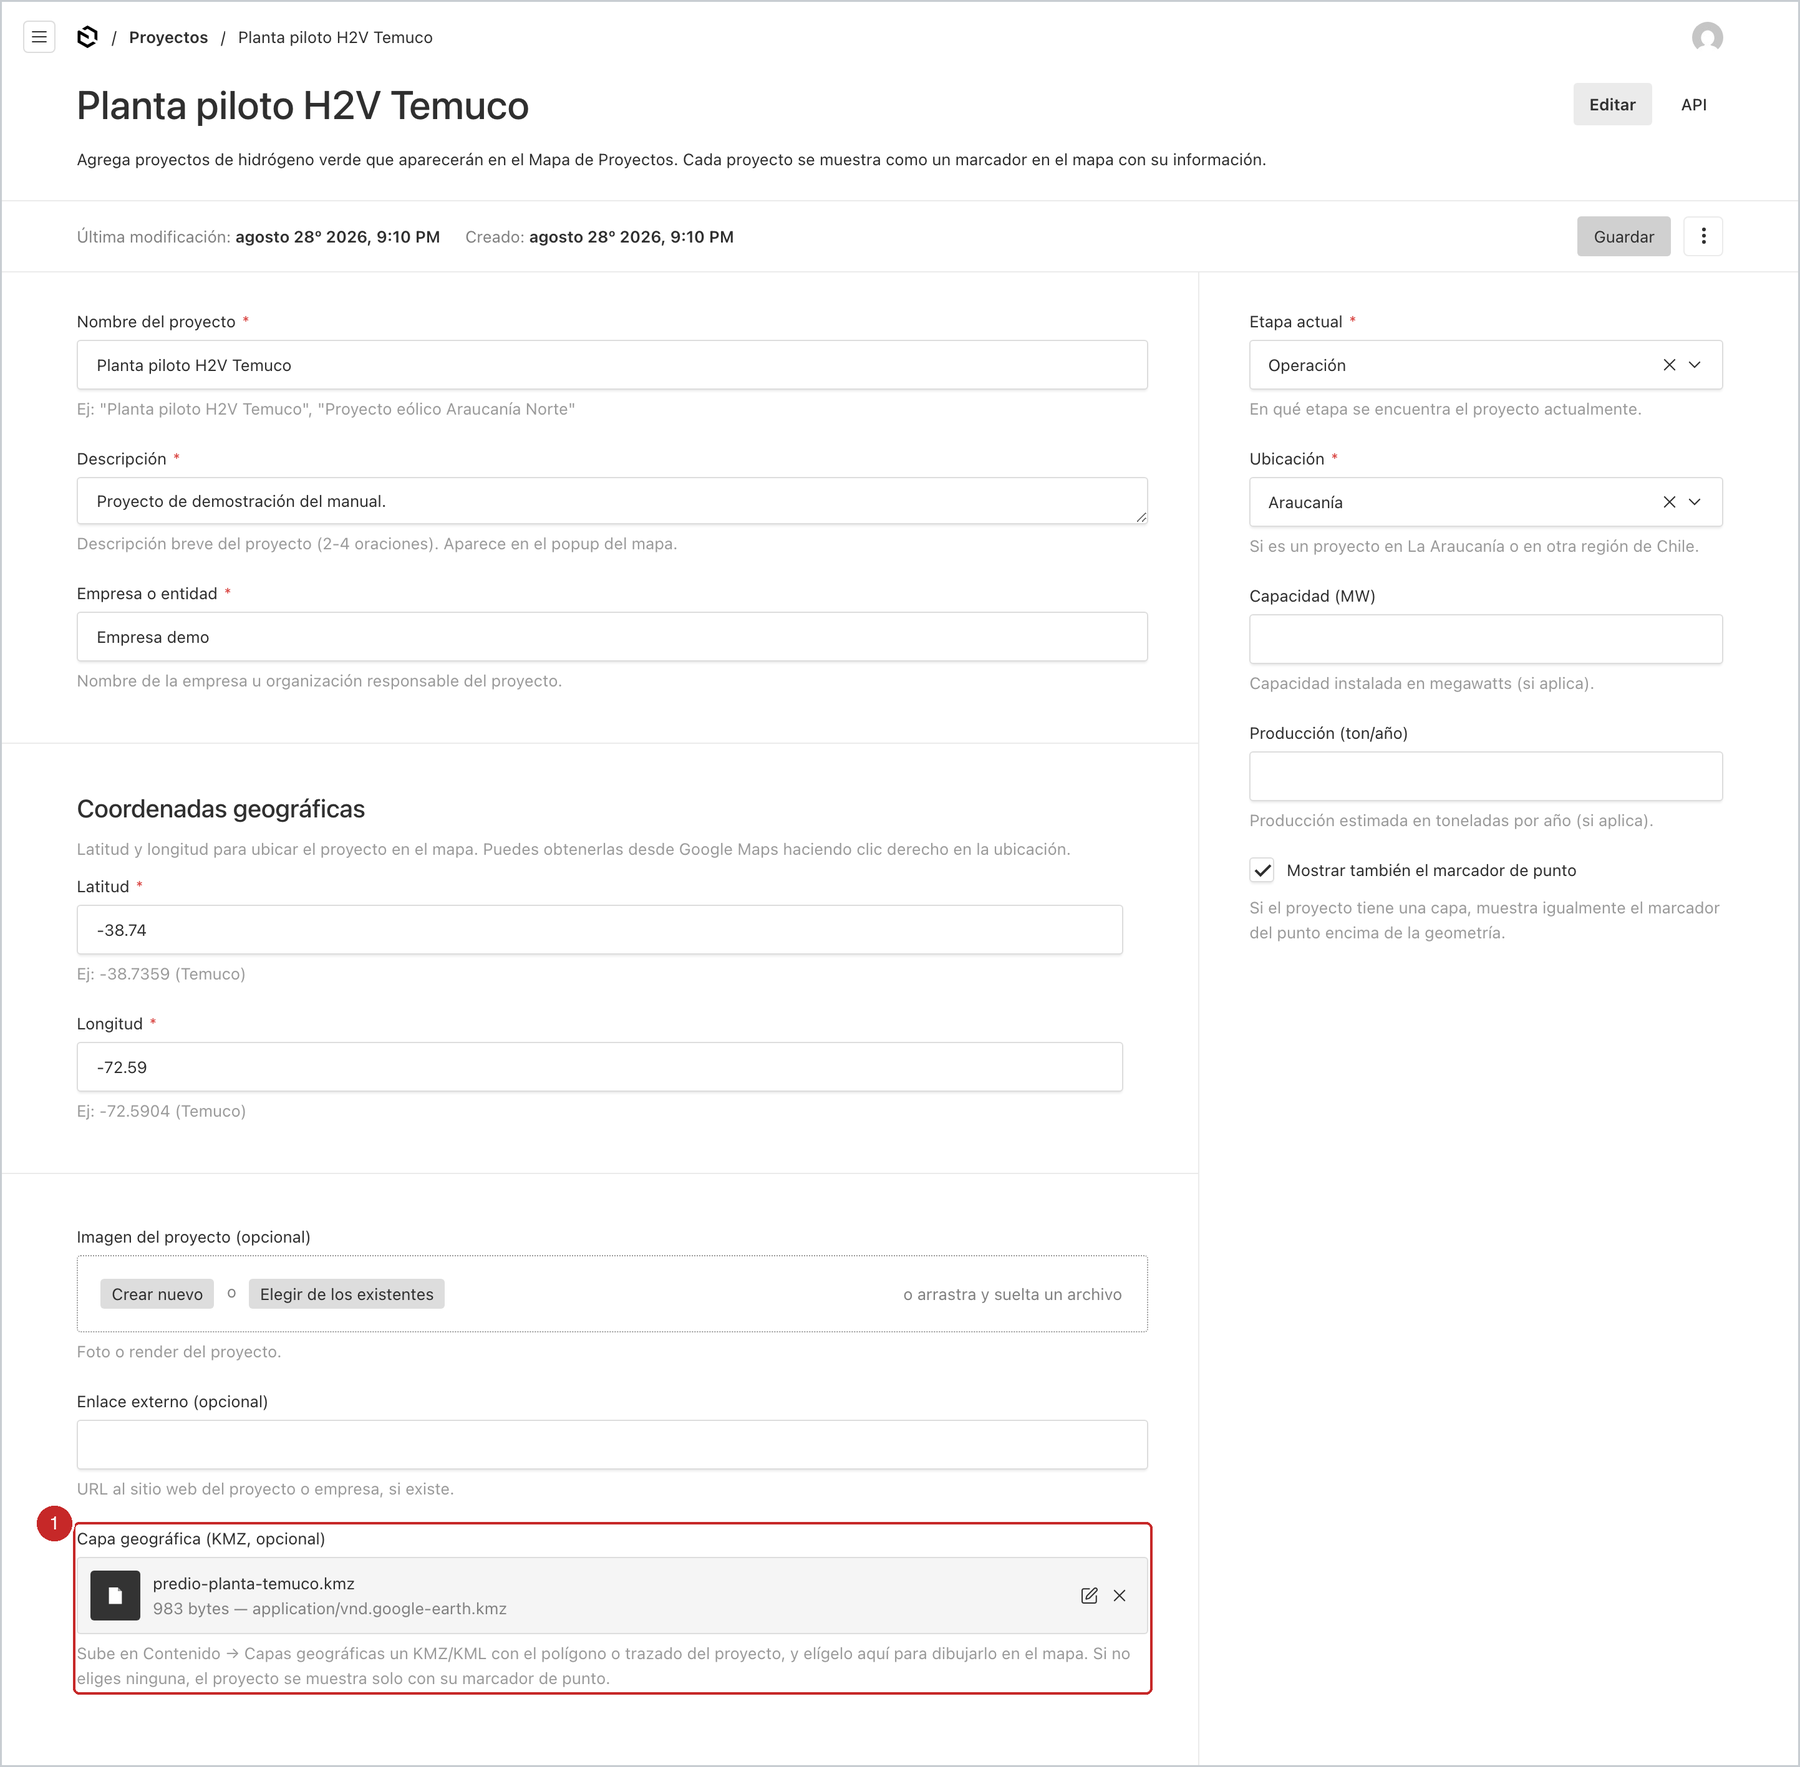
\includegraphics[width=\linewidth,keepaspectratio]{13c-proyecto-capa.png}
\caption{El campo ''Capa geográfica (KMZ, opcional)'' al final del formulario del proyecto (1), ya con la capa elegida.}
\end{figure}
\begin{recuadro}{cConsejo}{bConsejo}\textbf{\color{bConsejo}Consejo:} escriba las coordenadas del proyecto (Latitud y Longitud) de un punto \textbf{dentro} del terreno dibujado; así el círculo queda sobre la forma. En la columna derecha, la casilla \textbf{Mostrar también el marcador de punto} (marcada de fábrica) decide si se ve el círculo; desmárquela si prefiere ver solo la forma.\end{recuadro}
\subsection{Parte 4. Comprobar en el sitio}
\begin{enumerate}
  \item Abra el sitio y entre a \textbf{Proyectos}. Si ya tenía la página abierta, recárguela.
  \item Busque la forma en el lugar del proyecto. Para acercarse, use el filtro \textbf{Araucanía} que está bajo el mapa, o los botones \textbf{+} y \textbf{−} del mapa.
  \item Haga clic sobre la forma o sobre el círculo: se abre la ficha del proyecto.
\end{enumerate}
Sobre el mapa también aparecen los botones \textbf{Descargar todos (KMZ)} y \textbf{Abrir en Google Earth} (1): con ellos cualquier visitante se lleva los proyectos a Google Earth, sin que usted tenga que hacer nada. El ícono de capas (2), arriba a la derecha del mapa, cambia a la vista satelital.

\begin{figure}[H]\centering
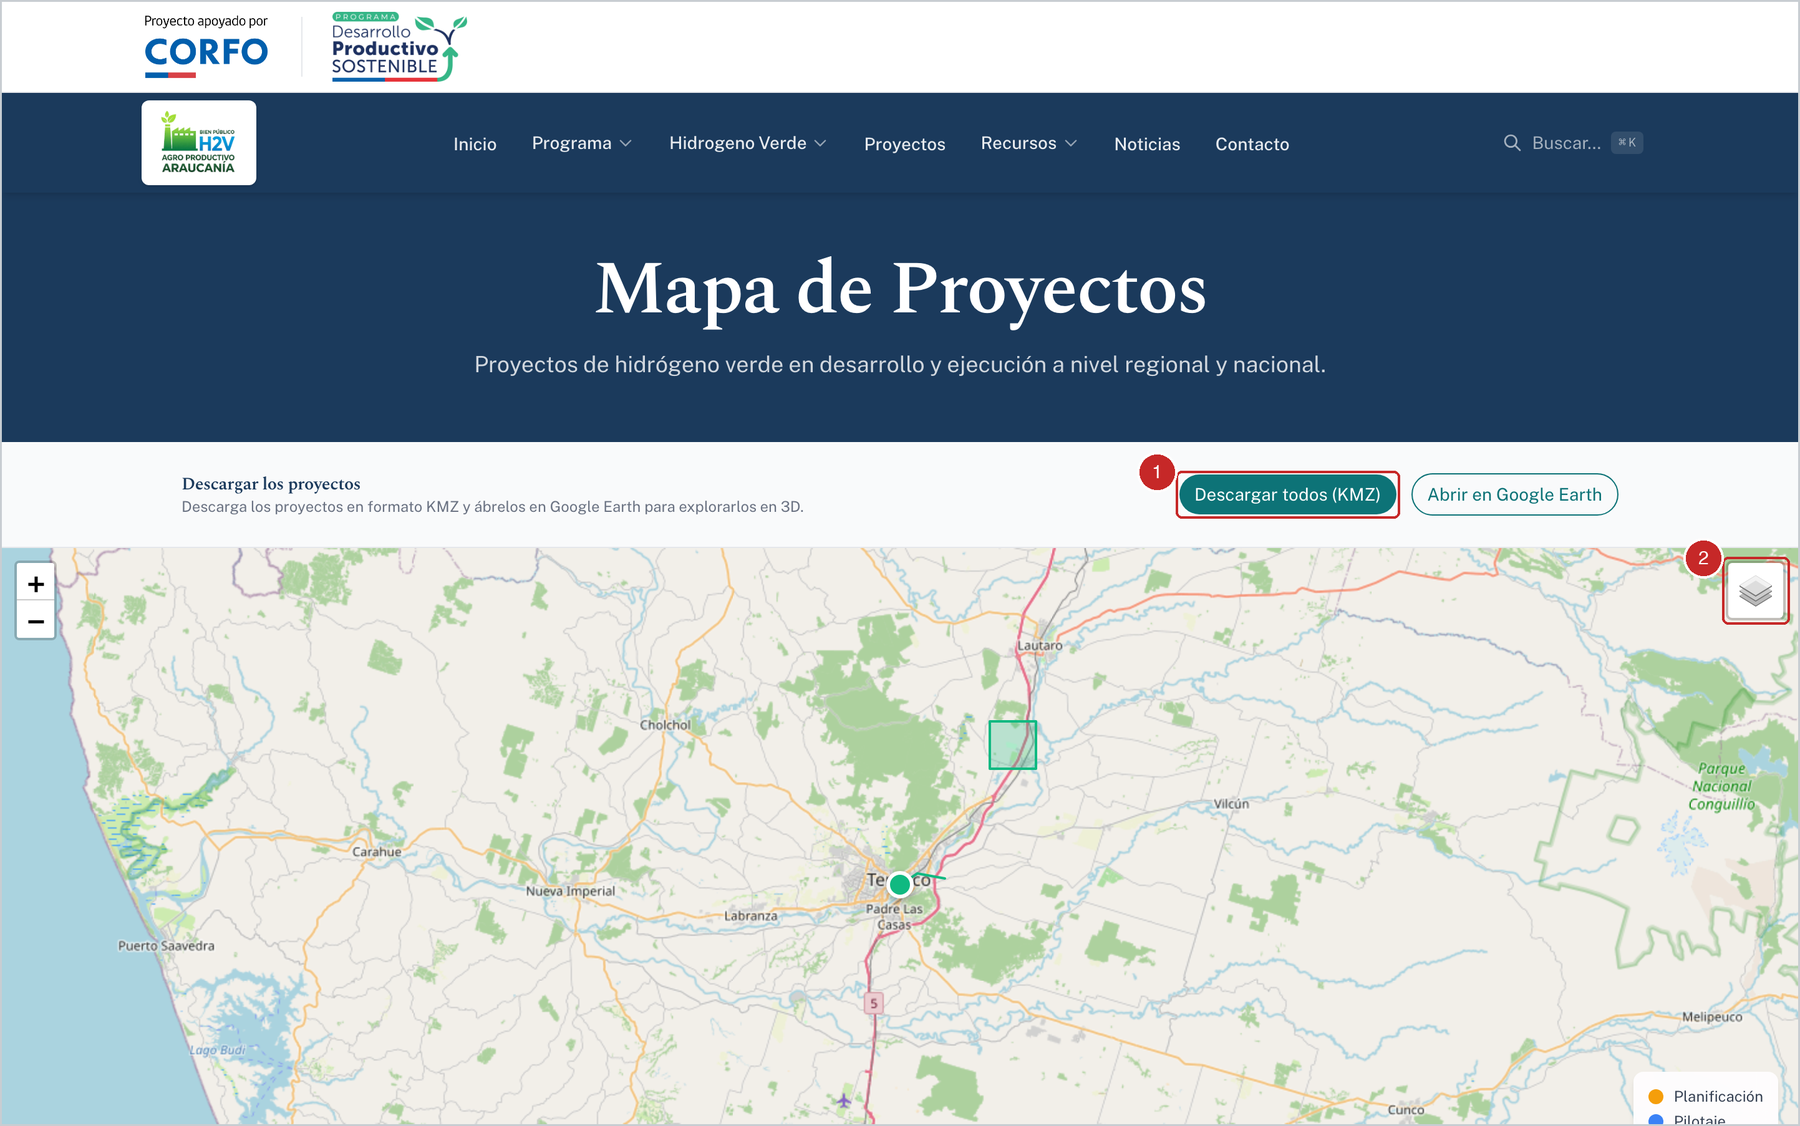
\includegraphics[width=\linewidth,keepaspectratio]{46b-web-proyectos-kmz.png}
\caption{El mapa público con la forma del proyecto dibujada, los botones de descarga (1) y el ícono de capas (2).}
\end{figure}
\begin{recuadro}{cNota}{bNota}\textbf{\color{bNota}Nota:} si no ve los botones de descarga ni la forma, las funciones de mapa están apagadas. No es un error suyo ni del panel: las enciende el equipo informático (Anexo D). Hoy están encendidas.\end{recuadro}
\subsection{Cambiar o quitar la forma de un proyecto}
\begin{itemize}
  \item \textbf{Cambiarla por otra:} suba el archivo nuevo como una capa nueva (Parte 2) y, en el proyecto, elija esa capa nueva (Parte 3). Después puede eliminar la capa antigua.
  \item \textbf{Quitarla del mapa:} abra el proyecto, en el campo \textbf{Capa geográfica (KMZ, opcional)} haga clic en la \textbf{X} que está junto a la capa, y guarde. El proyecto vuelve a verse solo con su círculo.
  \item \textbf{Eliminar una capa del panel} (solo Administrador): primero quítela de los proyectos que la usan; luego ábrala en \textbf{Capas geográficas (KMZ)}, haga clic en los tres puntos junto a \textbf{Guardar} y elija \textbf{Eliminar}.
\end{itemize}
\begin{recuadro}{cConsejo}{bConsejo}\textbf{\color{bConsejo}Consejo:} una capa también puede servir de \textbf{contexto} para toda la región; por ejemplo, todos los proyectos del SEIA en La Araucanía exportados como KMZ. Súbala con \textbf{Tipo de capa = ''Capa de referencia (contexto)''} y no la una a ningún proyecto. Aparece \textbf{apagada} en el ícono de capas del mapa, y cada visitante decide si la enciende.\end{recuadro}
\begin{recuadro}{cAtencion}{bAtencion}\textbf{\color{bAtencion}Atención:} cada archivo puede pesar \textbf{hasta 4 MB} y el sitio acepta \textbf{hasta 50 capas} en total. El sitio es de difusión: suba formas acotadas al proyecto, no mapas completos.\end{recuadro}
\section{Actualizar la gobernanza (personas)}
Las personas de la gobernanza se administran en \textbf{Miembros de Gobernanza} y aparecen automáticamente en las páginas \textbf{Quiénes Somos} y \textbf{Gobernanza} del sitio, agrupadas en tres instancias:

\begin{itemize}
  \item \textbf{Consejo de Dirección (nivel estratégico)}: es el \textbf{Comité Estratégico del Bien Público} (presidido por la SEREMI de Energía, con vicepresidencia de CORFO). Se muestra como tabla con institución, cargo, titular y aporte.
  \item \textbf{Comité Consultivo Técnico Científico}.
  \item \textbf{Unidad de Coordinación y Gestión (nivel operativo)}: el equipo del proyecto. Mientras un cargo no tenga titular, se deja con el nombre ''Por definir''.
\end{itemize}
Para agregar una persona:

\begin{enumerate}
  \item Menú lateral $\rightarrow$ \textbf{Miembros de Gobernanza} $\rightarrow$ \textbf{Crear nuevo}.
  \item Complete:
\end{enumerate}
\begin{longtable}{>{\raggedright\arraybackslash}p{0.203\textwidth}>{\raggedright\arraybackslash}p{0.572\textwidth}>{\raggedright\arraybackslash}p{0.155\textwidth}}
\rowcolor{h2vazul}\textbf{\color{white}Campo} & \textbf{\color{white}Qué escribir} & \textbf{\color{white}Obligatorio} \\
\endfirsthead
\rowcolor{h2vazul}\textbf{\color{white}Campo} & \textbf{\color{white}Qué escribir} & \textbf{\color{white}Obligatorio} \\
\endhead
\textbf{Nombre completo} & Nombre y apellido (o ''Por definir'' si el cargo está vacante). & Sí \\ \midrule
\rowcolor{filaalt}\textbf{Cargo} & Ejemplo: ''Presidente'', ''Vicepresidenta'', ''Miembro Titular'', ''Secretaría Técnica'', ''Director del proyecto''. Máximo 60 caracteres. & Sí \\ \midrule
\textbf{Institución} & La organización que representa. Ejemplo: ''Ministerio de Energía — Seremi Araucanía'', ''CORFO'', ''CODESSER'', ''Universidad de Talca''. & Sí \\ \midrule
\rowcolor{filaalt}\textbf{Instancia de gobernanza} (barra lateral) & A cuál de las tres instancias pertenece. & Sí \\ \midrule
\textbf{Foto} & Foto de perfil cuadrada (mínimo 200 x 200). & No \\ \midrule
\rowcolor{filaalt}\textbf{Aporte al programa} & Una frase: cómo contribuye. & No \\ \midrule
\textbf{Nombre del suplente} & Si tiene suplente. & No \\ \midrule
\rowcolor{filaalt}\textbf{Orden de aparición} (barra lateral) & Número para ordenar: 1 aparece primero, 2 después, etc. & No \\ \bottomrule
\end{longtable}
\begin{enumerate}[start=3]
  \item Pulse \textbf{Guardar}.
\end{enumerate}
\begin{figure}[H]\centering
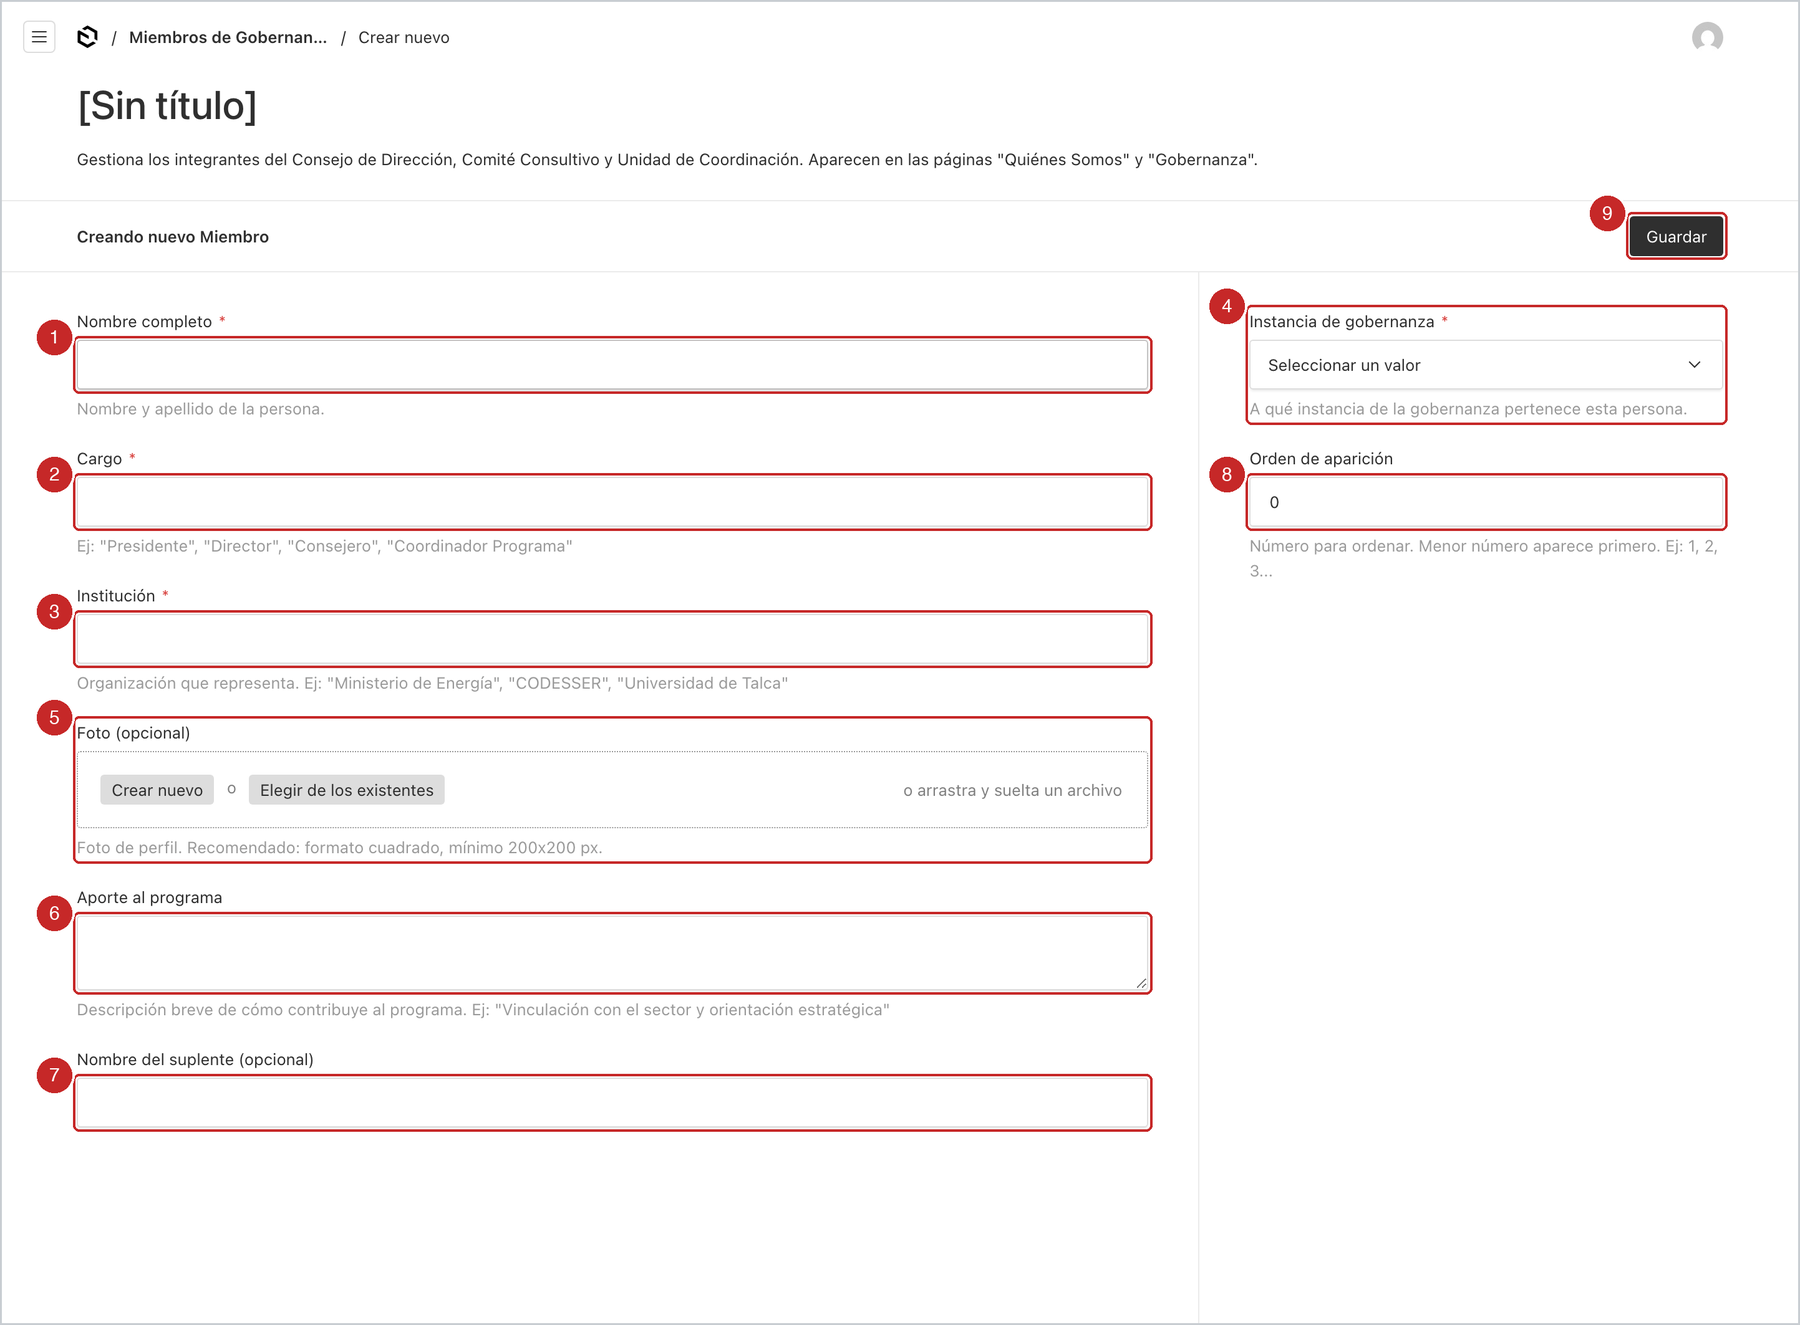
\includegraphics[width=\linewidth,keepaspectratio]{14-miembro-crear.png}
\caption{Formulario de un miembro de gobernanza: nombre (1), cargo (2), institución (3), instancia (4), foto (5), aporte (6), suplente (7), orden (8) y Guardar (9).}
\end{figure}
Para \textbf{cambiar a una persona por otra} (por ejemplo, un nuevo titular en el Comité), no cree una fila nueva: abra la fila de ese cargo, cambie el nombre (y el suplente o la foto si corresponde) y guarde. Así se mantiene el orden de la tabla.

\begin{figure}[H]\centering
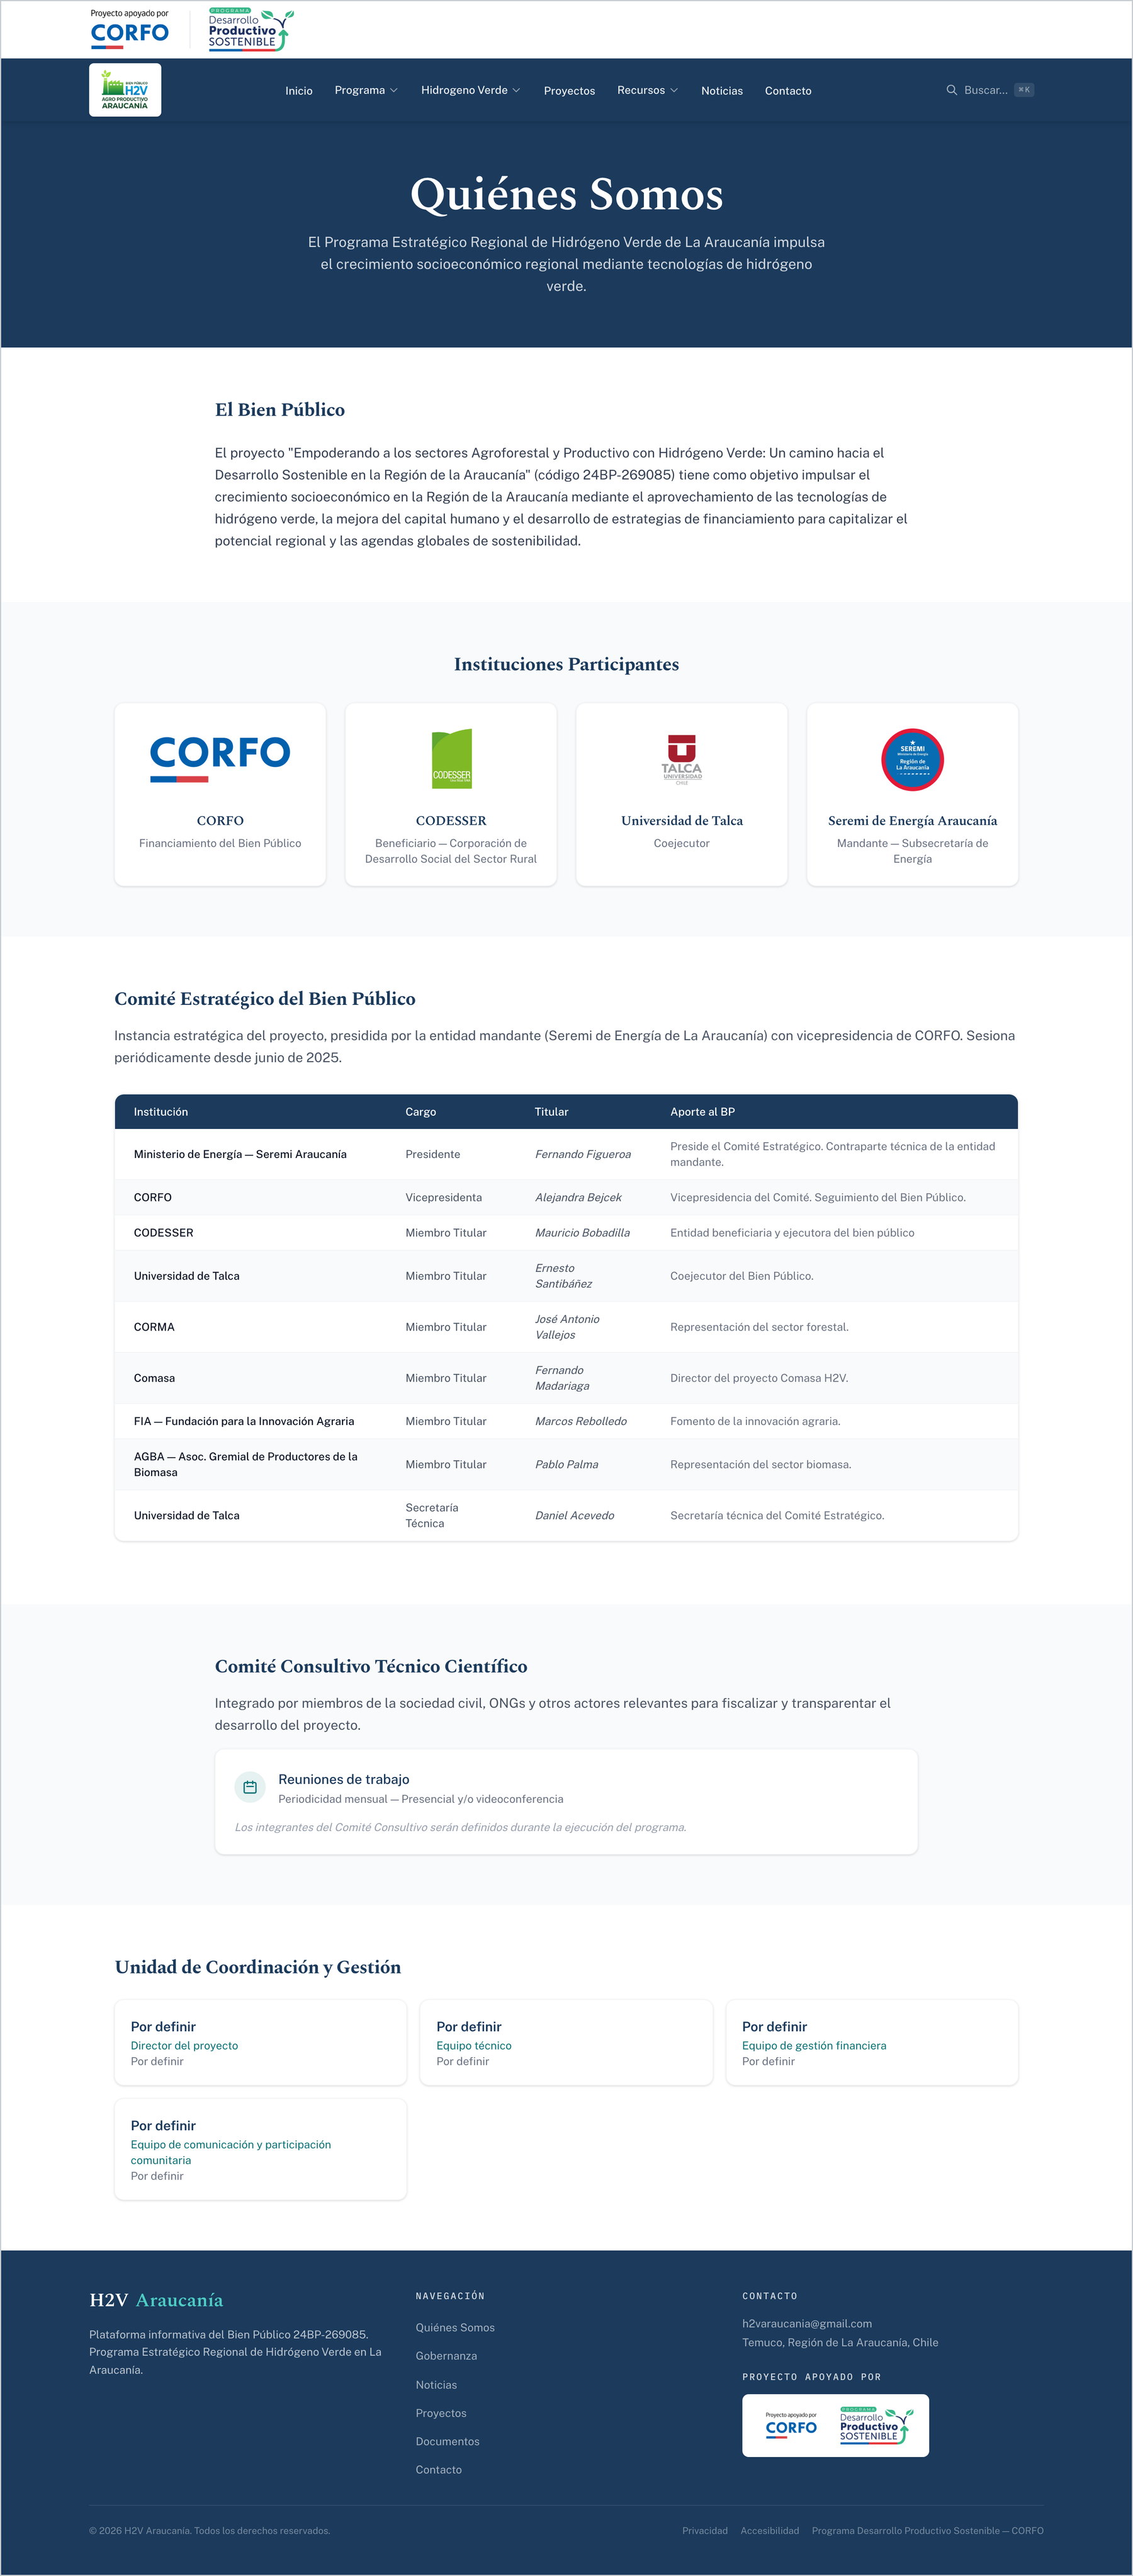
\includegraphics[width=\linewidth,height=0.74\textheight,keepaspectratio]{41-web-quienes-somos.png}
\caption{Así se ve la página Quiénes Somos del sitio, con las instituciones y la tabla del Comité Estratégico.}
\end{figure}
\begin{figure}[H]\centering
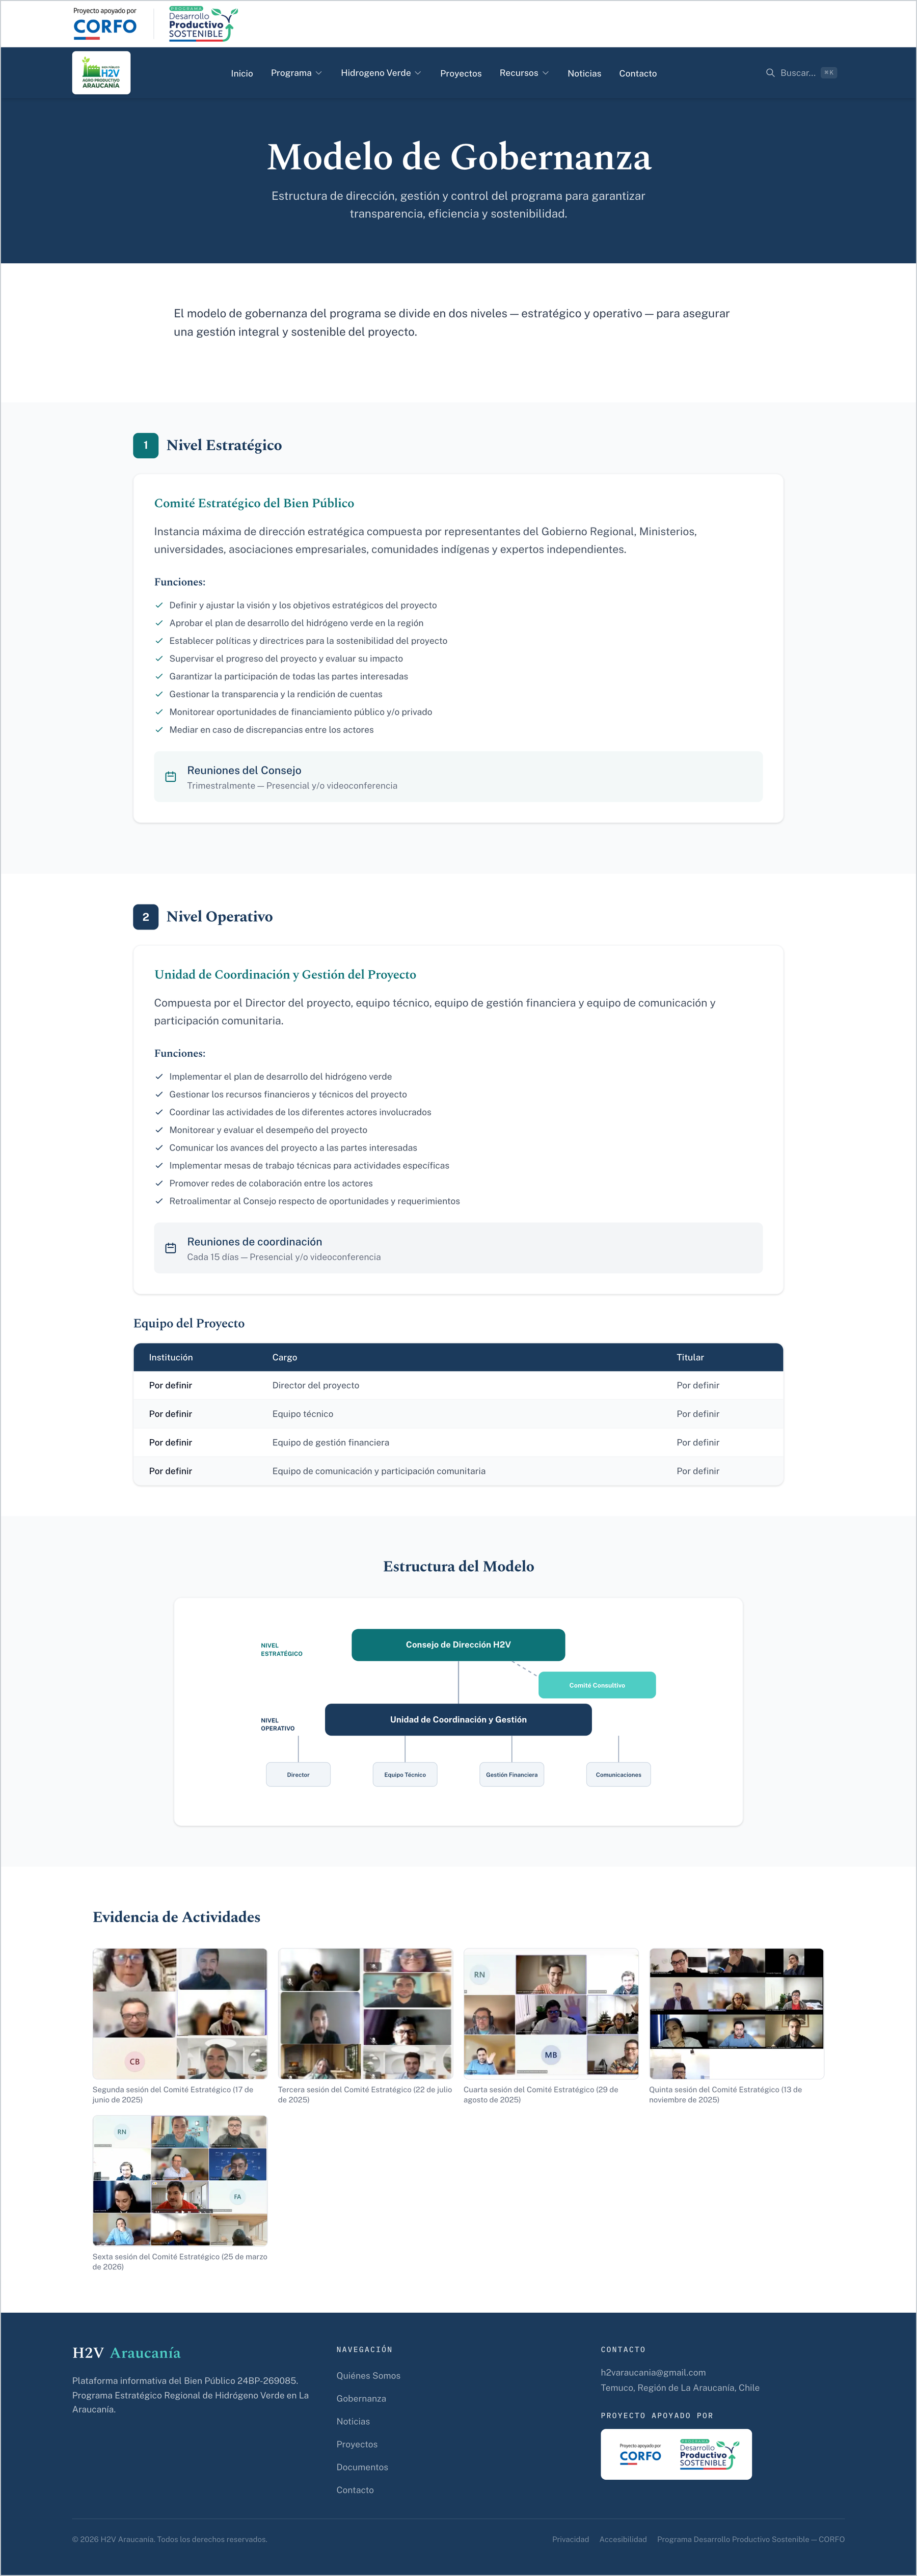
\includegraphics[width=\linewidth,height=0.74\textheight,keepaspectratio]{42-web-gobernanza.png}
\caption{Así se ve la página Gobernanza del sitio, con los niveles, el equipo del proyecto y el diagrama.}
\end{figure}
\section{Subir fotos de actividades (galería de Gobernanza)}
La página Gobernanza tiene una galería ''Evidencia de Actividades'' (fotos de sesiones del Comité, talleres, visitas).

\begin{enumerate}
  \item Menú lateral $\rightarrow$ grupo \textbf{Páginas} $\rightarrow$ \textbf{Gobernanza}.
  \item Baje hasta \textbf{Evidencia de Actividades (galería de fotos)} y pulse \textbf{Añadir fila}.
  \item Suba la \textbf{Foto} (ideal horizontal) y escriba una \textbf{Descripción breve} (ejemplo: ''Sesión del Comité Estratégico, junio 2026'').
  \item Repita para cada foto. Puede reordenarlas arrastrando el tirador de puntos de cada fila.
  \item Pulse \textbf{Guardar}.
\end{enumerate}
\section{Archivos multimedia}
En \textbf{Sistema $\rightarrow$ Archivos multimedia} están todos los archivos subidos al sitio (imágenes, PDF, logos), con su descripción. Desde aquí puede buscar un archivo, ver dónde está, subir archivos nuevos para usarlos después, o reemplazar una imagen.

\begin{figure}[H]\centering
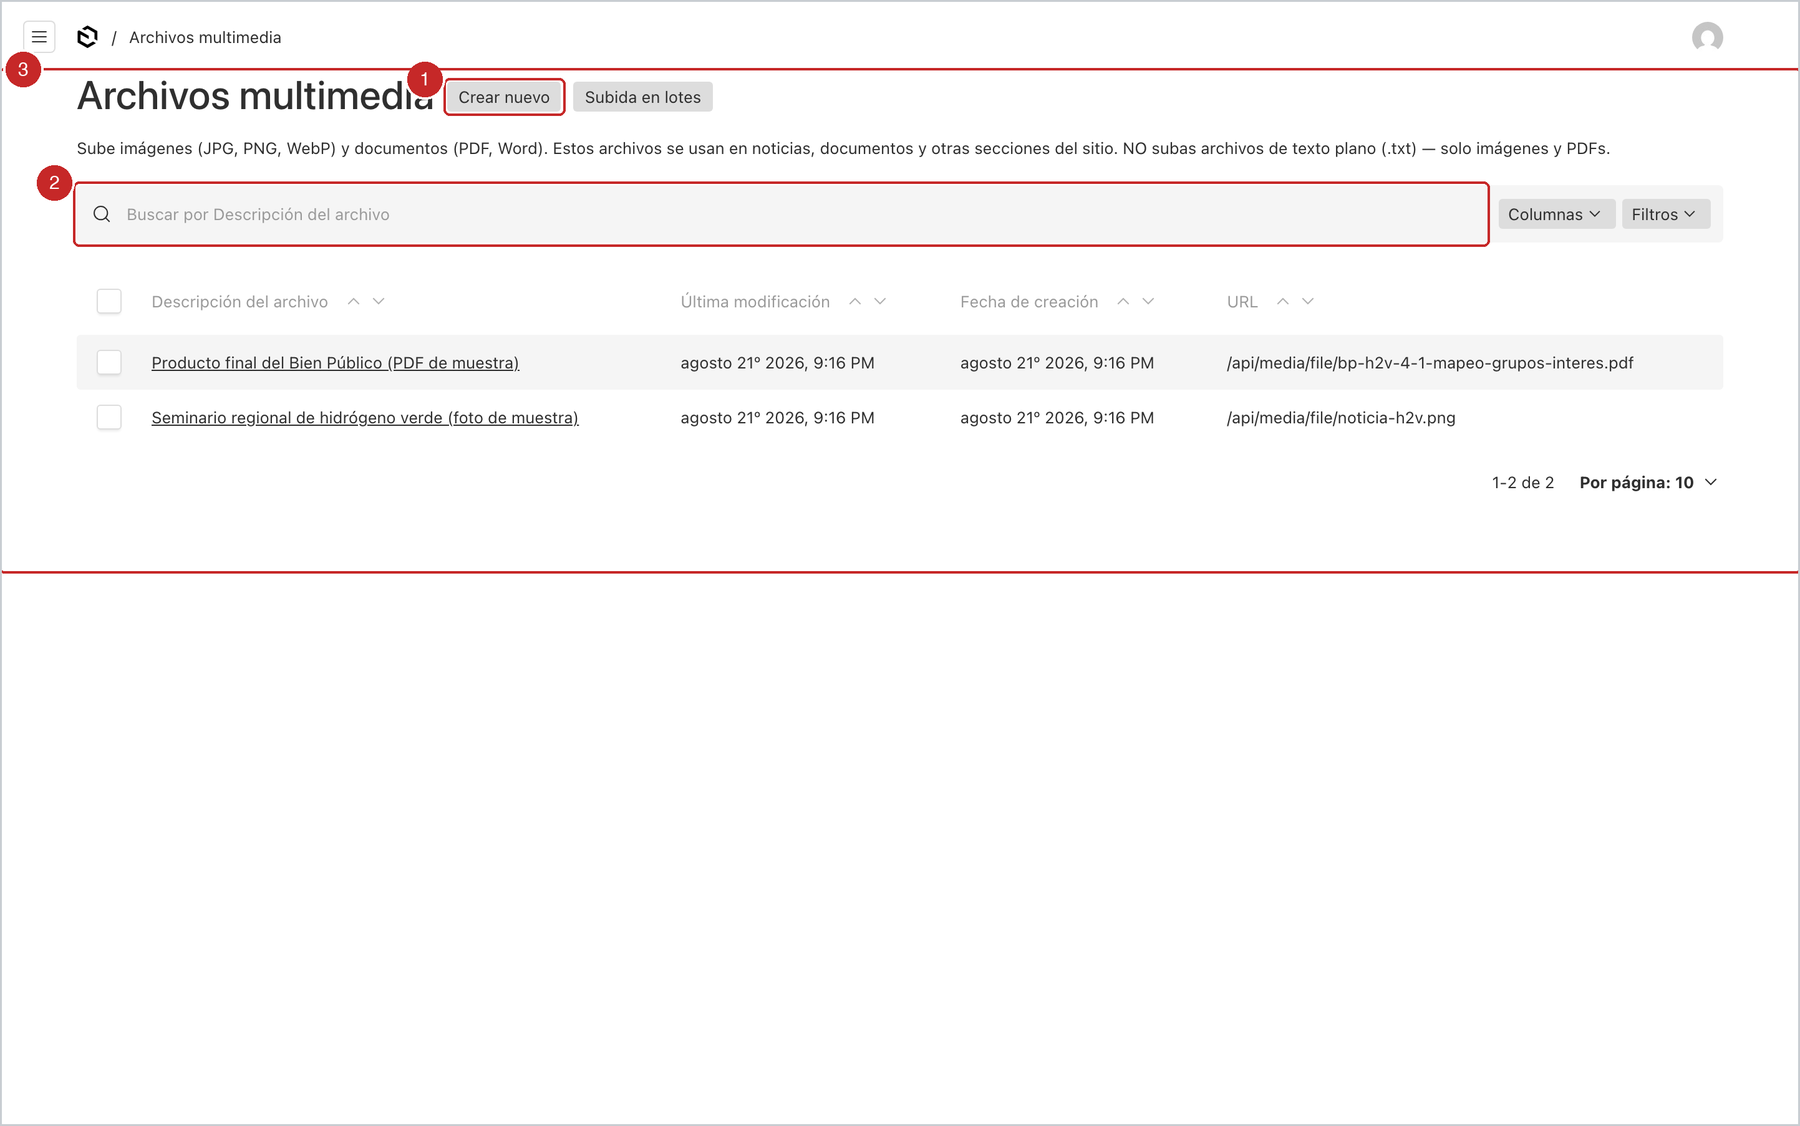
\includegraphics[width=\linewidth,keepaspectratio]{16-media-lista.png}
\caption{Lista de archivos multimedia: Crear nuevo (1), buscador (2) y los archivos (3).}
\end{figure}
\begin{figure}[H]\centering
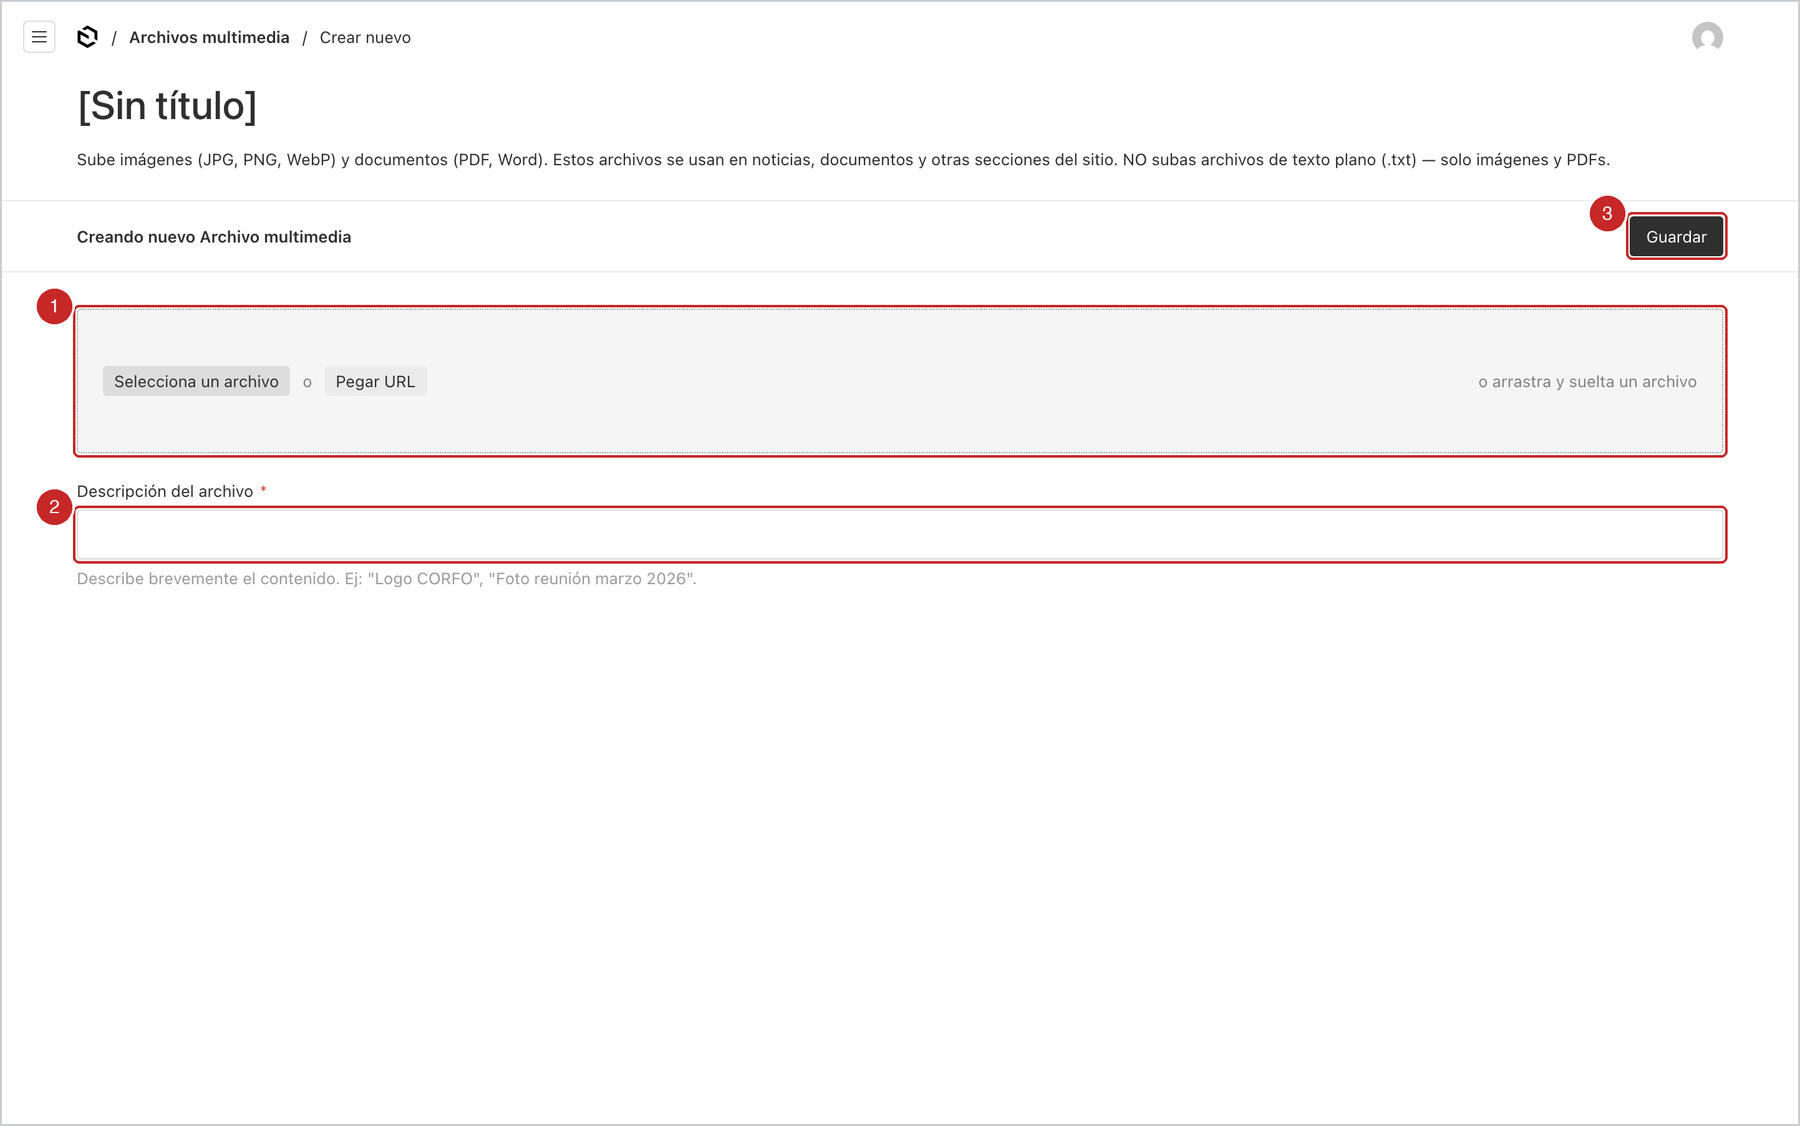
\includegraphics[width=\linewidth,keepaspectratio]{17-media-subir.png}
\caption{Subir un archivo desde Archivos multimedia: zona de subida (1), descripción obligatoria (2) y Guardar (3).}
\end{figure}
\begin{recuadro}{cAtencion}{bAtencion}\textbf{\color{bAtencion}Atención:} eliminar un archivo que está en uso (por ejemplo, la portada de una noticia) deja esa noticia sin imagen. Por eso solo los Administradores pueden eliminar archivos; antes de hacerlo, compruebe que no se usa.\end{recuadro}
\section{Leer los mensajes del formulario de Contacto}
Todo lo que los visitantes escriben en el formulario de la página \textbf{Contacto} queda guardado en el panel, aunque el aviso por correo no llegue.

\begin{enumerate}
  \item Menú lateral $\rightarrow$ grupo \textbf{Contenido} $\rightarrow$ \textbf{Mensajes de contacto} (1). Los mensajes más recientes aparecen primero (2).
  \item La columna \textbf{Atendido} (3) muestra cuáles ya se respondieron (''verdadero'') y cuáles no (''falso'').
\end{enumerate}
\begin{figure}[H]\centering
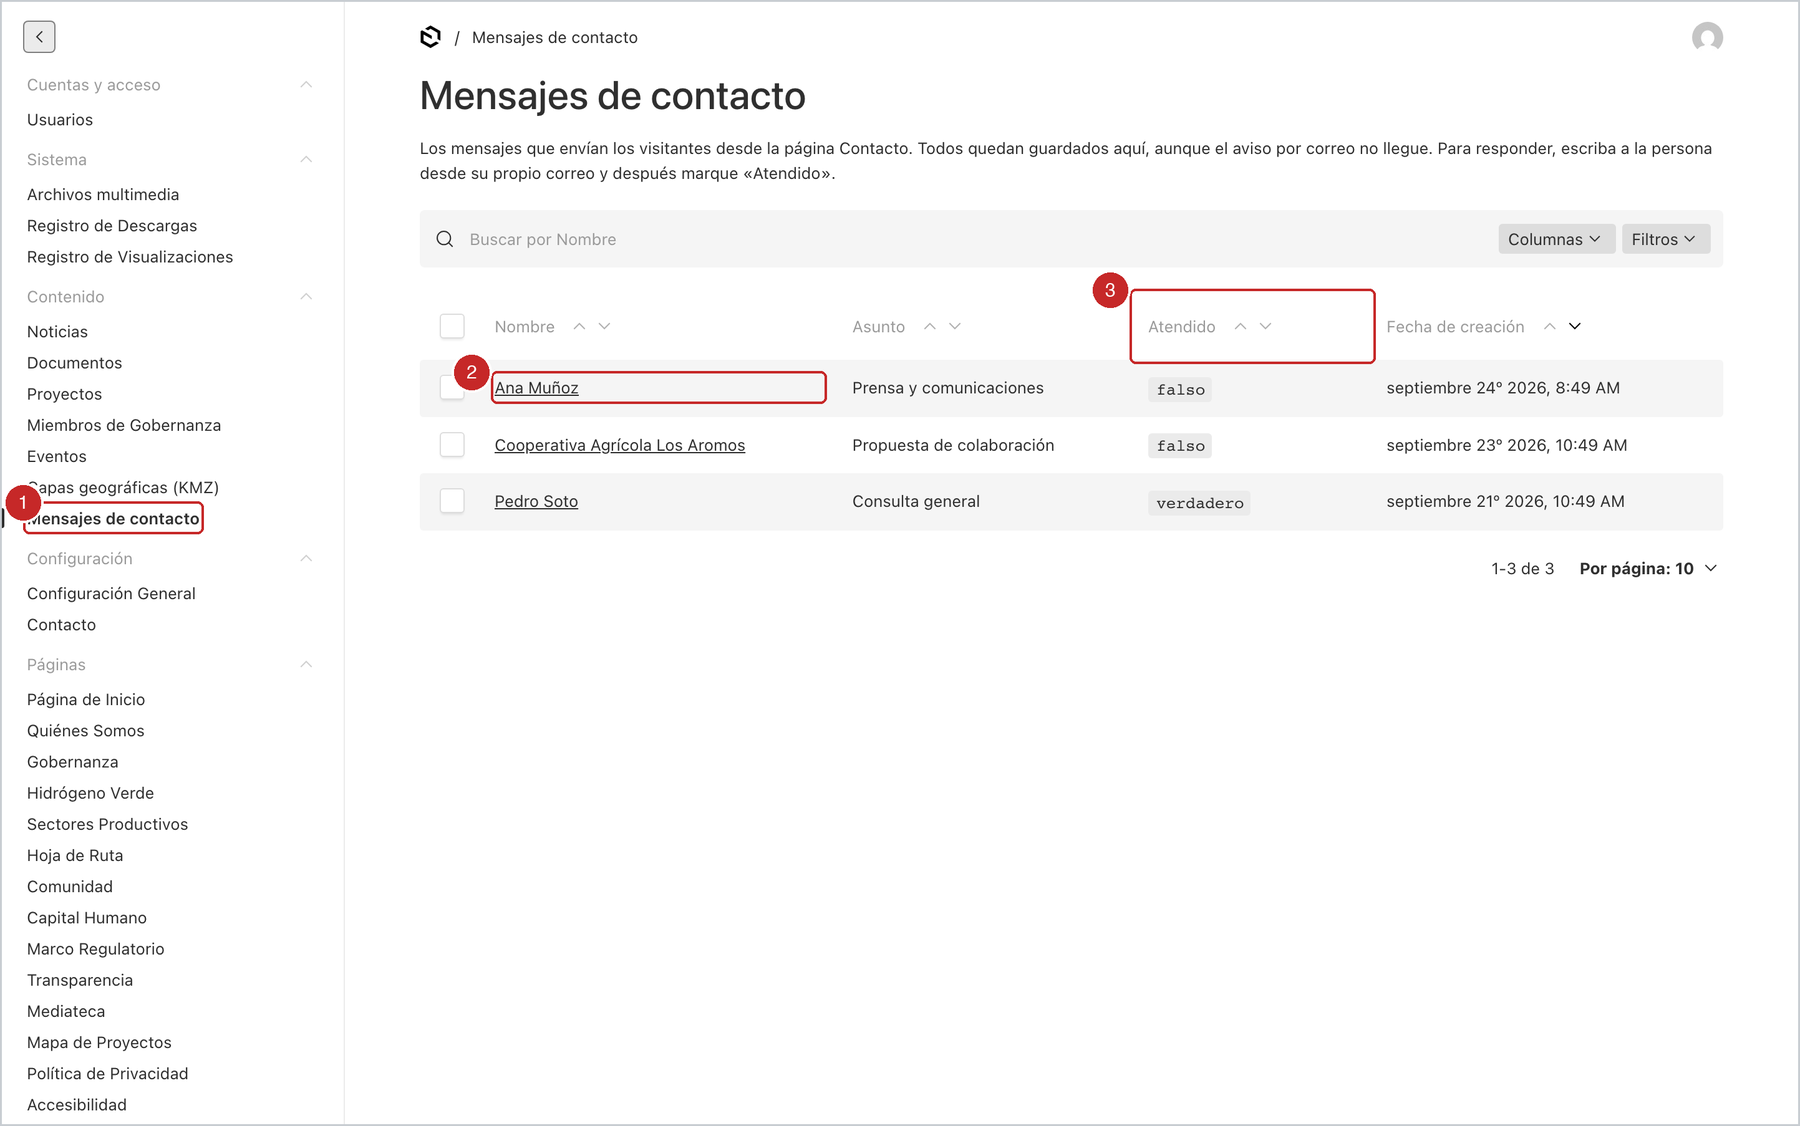
\includegraphics[width=\linewidth,keepaspectratio]{18-mensajes-lista.png}
\caption{Mensajes de contacto: dónde está en el menú (1), el mensaje más reciente (2) y la columna Atendido (3).}
\end{figure}
\begin{enumerate}[start=3]
  \item Haga clic en el nombre de la persona para abrir su mensaje (2).
  \item Para responder, escríbale desde su propio correo a la dirección que aparece en \textbf{Correo de la persona} (1). El panel no envía respuestas.
  \item Cuando haya respondido, marque \textbf{Atendido} (3) y pulse \textbf{Guardar} (5).
\end{enumerate}
\begin{figure}[H]\centering
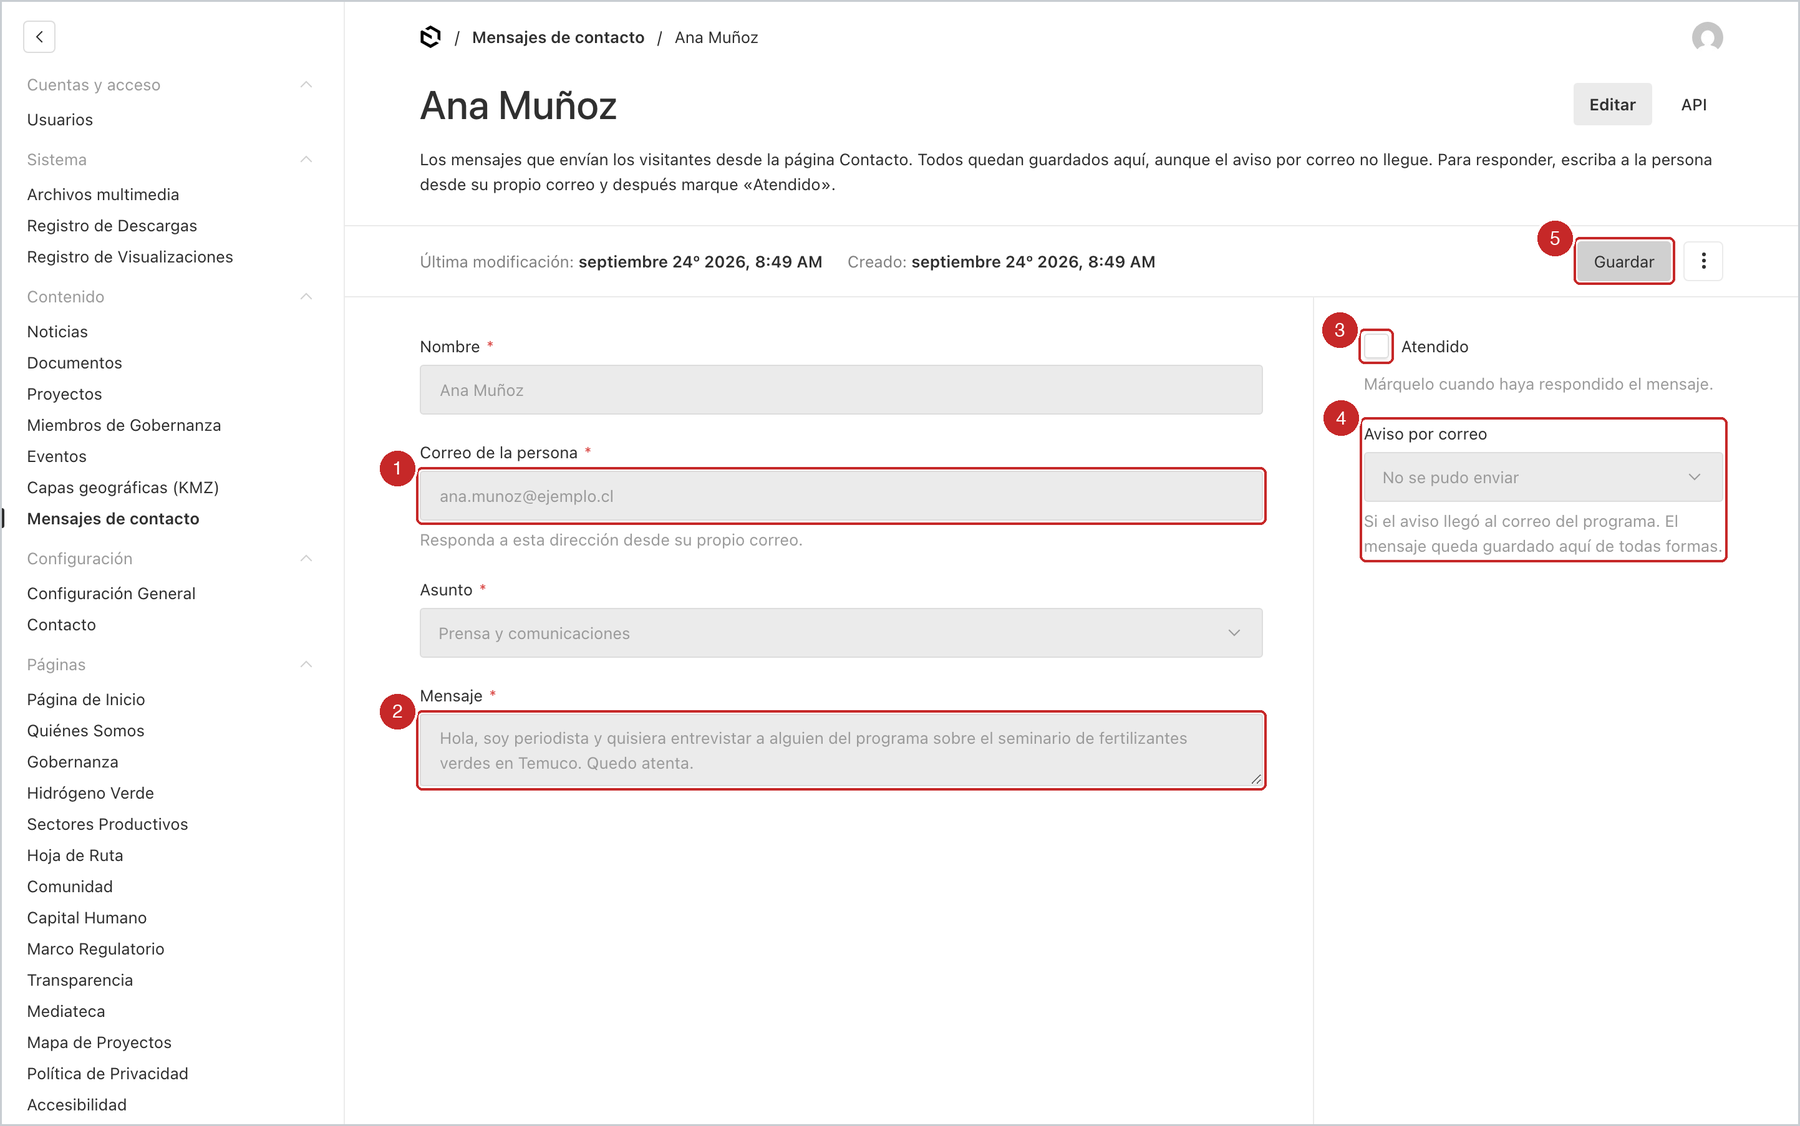
\includegraphics[width=\linewidth,keepaspectratio]{19-mensaje-detalle.png}
\caption{Un mensaje abierto: correo de la persona (1), mensaje (2), casilla Atendido (3), si el aviso por correo llegó (4) y Guardar (5).}
\end{figure}
\begin{recuadro}{cConsejo}{bConsejo}\textbf{\color{bConsejo}Consejo:} revise esta sección una o dos veces por semana. Mientras el sitio no tenga dominio propio, el aviso por correo puede no llegar; el campo \textbf{Aviso por correo} (4) indica si llegó.\end{recuadro}
\begin{recuadro}{cSeguridad}{bSeguridad}\textbf{\color{bSeguridad}Seguridad:} los mensajes contienen datos personales (el nombre y el correo de quien escribe). Úselos solo para responder y no los comparta. Solo un Administrador puede eliminarlos.\end{recuadro}
\chapter{Editar los textos de cada página}
\section{Cómo funcionan las Páginas}
En el grupo \textbf{Páginas} del menú hay un formulario por cada página del sitio. Cada formulario está dividido en secciones con el mismo nombre que las partes de la página pública (Encabezado, Sección Hero, Banda de indicadores...). Tres reglas:

\begin{itemize}
  \item Lo que usted escribe \textbf{reemplaza} el texto estándar del sitio. Lo que deja \textbf{vacío} muestra el texto estándar (así nunca queda un hueco).
  \item Las secciones con varios elementos (cifras, tarjetas, hitos, logos, fotos) son \textbf{listas}: tienen un botón \textbf{Añadir ...} al final, y cada fila tiene un menú de tres puntos (mover, duplicar, eliminar) y un tirador de puntos para arrastrar y reordenar. Los botones \textbf{Contraer Todo / Mostrar Todo} ayudan cuando la lista es larga.
  \item Al pulsar \textbf{Guardar}, el cambio se ve en el sitio de inmediato (estas páginas no tienen borrador).
\end{itemize}
\begin{recuadro}{cConsejo}{bConsejo}\textbf{\color{bConsejo}Consejo:} abra el sitio público en otra pestaña del navegador. Edite, guarde, recargue la pestaña del sitio y compruebe cómo quedó. Si no le gusta, vuelva a editar y guardar.\end{recuadro}
\section{Página de Inicio (la portada)}
Menú lateral $\rightarrow$ \textbf{Páginas $\rightarrow$ Página de Inicio}. Secciones del formulario y a qué corresponden en la portada:

\begin{longtable}{>{\raggedright\arraybackslash}p{0.287\textwidth}>{\raggedright\arraybackslash}p{0.643\textwidth}}
\rowcolor{h2vazul}\textbf{\color{white}Sección del formulario} & \textbf{\color{white}Qué controla en la portada} \\
\endfirsthead
\rowcolor{h2vazul}\textbf{\color{white}Sección del formulario} & \textbf{\color{white}Qué controla en la portada} \\
\endhead
\textbf{Sección Hero (banner principal)} & Línea superior (eyebrow) en mayúsculas pequeñas, Título grande, Subtítulo, y los textos de los dos botones (Cta Primario, Cta Secundario). \\ \midrule
\rowcolor{filaalt}\textbf{Banda de indicadores (KPIs)} & Las cifras destacadas bajo el banner (por ejemplo ''9 Instituciones'', ''88.745 t/año Demanda H2V al 2045'', ''32 Comunas'', ''2024–2050 Hoja de ruta''). Cada indicador tiene Cifra, Unidad (opcional) y Etiqueta. Se pueden agregar, quitar y reordenar. \\ \midrule
\textbf{Sección ''Explora el Programa''} & El kicker (palabra pequeña sobre el título), el título y las \textbf{Tarjetas de acceso rápido} (título, descripción y enlace de cada tarjeta). \\ \midrule
\rowcolor{filaalt}\textbf{Sección ''Últimas Noticias''} & Kicker, título y texto del enlace ''ver todas''. (Las noticias en sí vienen de Contenido $\rightarrow$ Noticias.) \\ \midrule
\textbf{Sección de logos institucionales} & Los títulos ''Proyecto apoyado por'' e ''Instituciones participantes''. (Los logos de las instituciones se cambian en Configuración General.) \\ \bottomrule
\end{longtable}
\begin{figure}[H]\centering
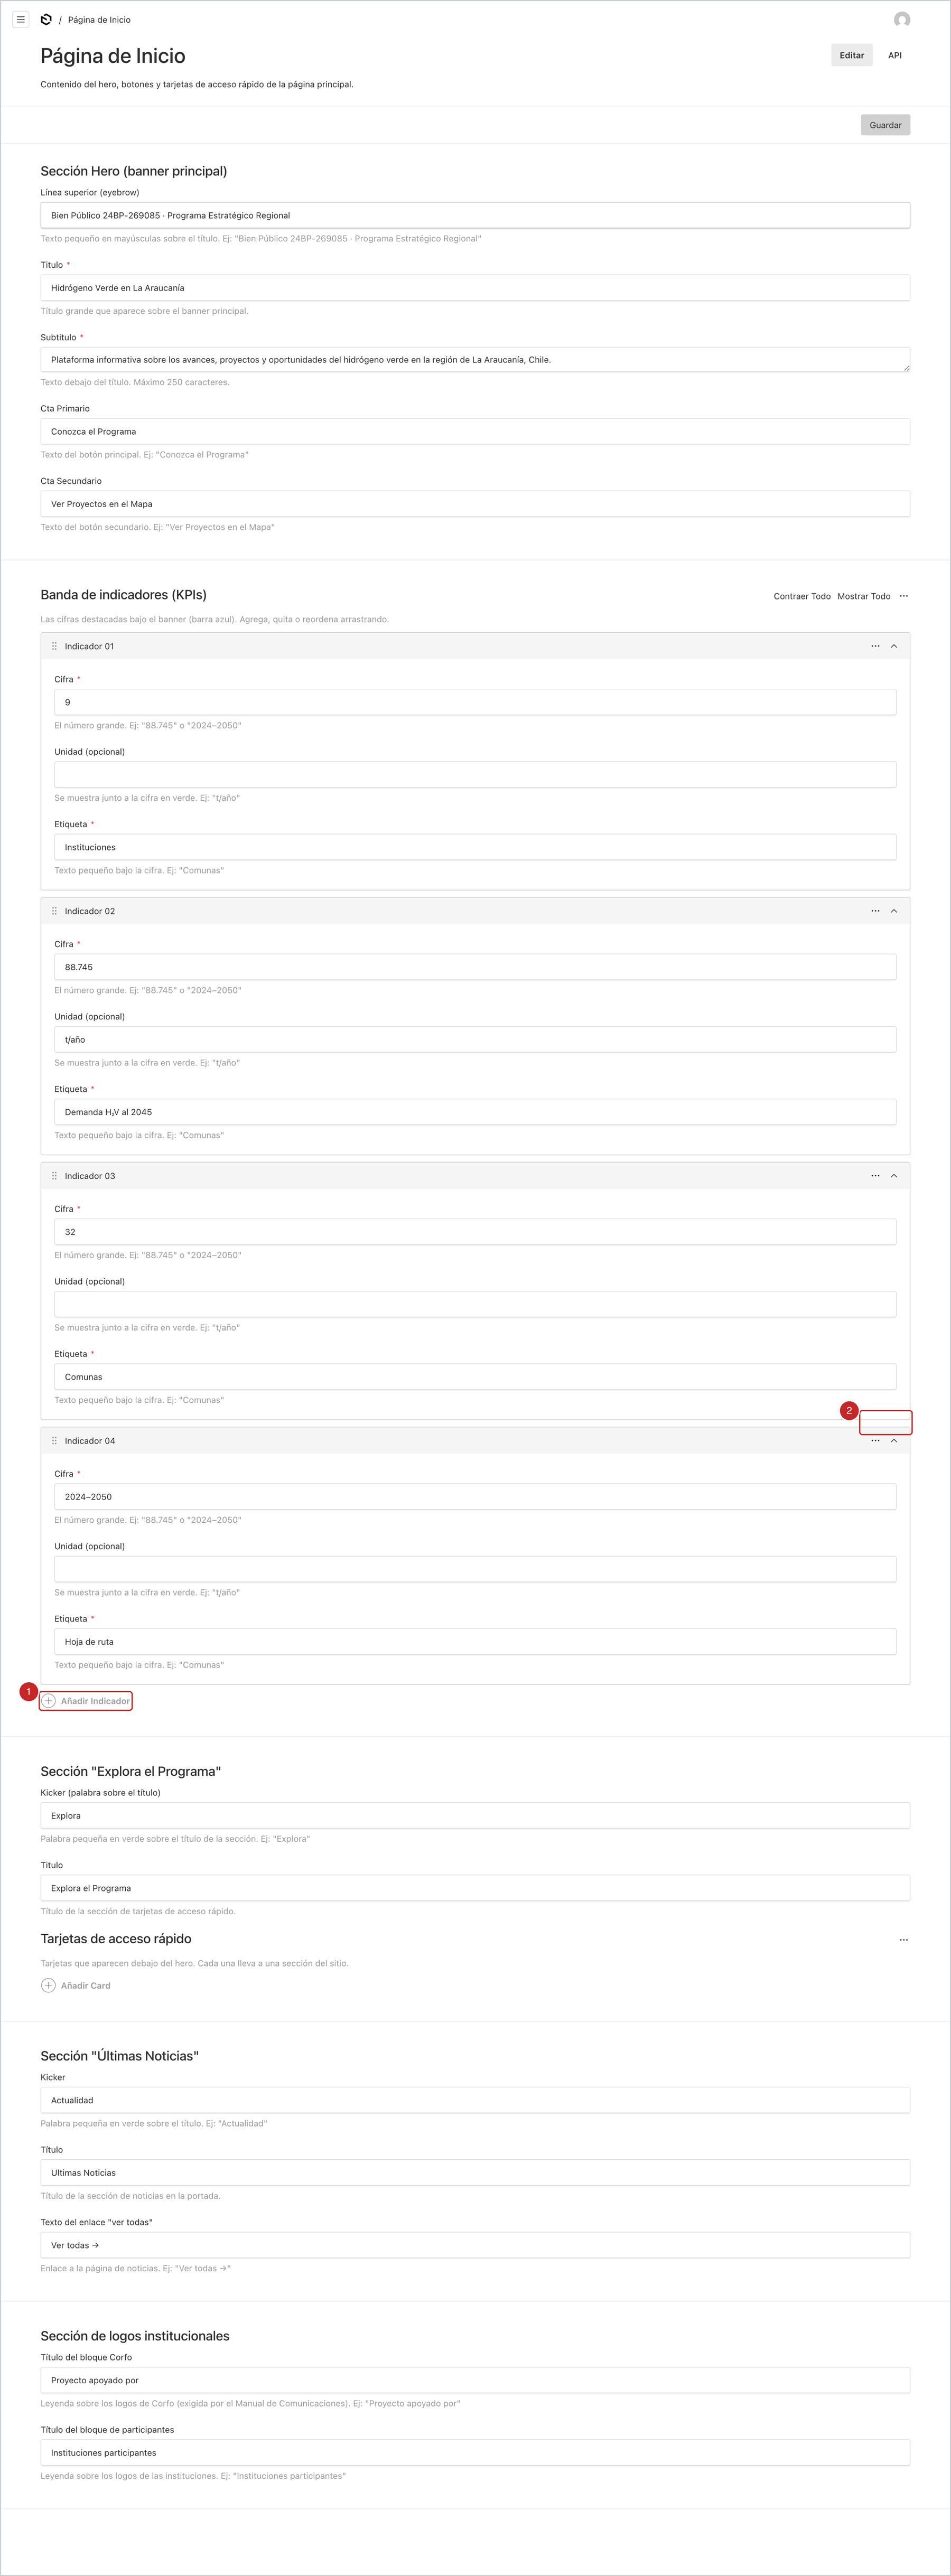
\includegraphics[width=\linewidth,height=0.74\textheight,keepaspectratio]{20-pagina-inicio.png}
\caption{Formulario completo de la Página de Inicio. Al final de cada lista está el botón Añadir (1); el botón Guardar (2) está arriba a la derecha.}
\end{figure}
\begin{recuadro}{cAtencion}{bAtencion}\textbf{\color{bAtencion}Atención:} los indicadores (KPIs) son cifras oficiales del programa. Antes de cambiarlos, confirme el dato con la Unidad de Coordinación.\end{recuadro}
\section{Quiénes Somos}
Menú lateral $\rightarrow$ \textbf{Páginas $\rightarrow$ Quiénes Somos}.

\begin{longtable}{>{\raggedright\arraybackslash}p{0.235\textwidth}>{\raggedright\arraybackslash}p{0.695\textwidth}}
\rowcolor{h2vazul}\textbf{\color{white}Sección} & \textbf{\color{white}Qué controla} \\
\endfirsthead
\rowcolor{h2vazul}\textbf{\color{white}Sección} & \textbf{\color{white}Qué controla} \\
\endhead
\textbf{Encabezado} & Título y subtítulo del banner azul. \\ \midrule
\rowcolor{filaalt}\textbf{El Bien Público} & Título y texto libre (editor de texto) que describe el proyecto. \\ \midrule
\textbf{Instituciones participantes} & Lista de instituciones con nombre, rol según las bases (por ejemplo CORFO: financiamiento; CODESSER: Beneficiario; Universidad de Talca: Coejecutor; Seremi de Energía: Mandante) y logo opcional. Si no sube logo, el sitio usa el logo oficial que ya tiene guardado para CORFO, CODESSER, UTalca y Seremi. \\ \midrule
\rowcolor{filaalt}\textbf{Título y Descripción del Consejo} & Título y texto de presentación de la tabla del Comité Estratégico. \\ \midrule
\textbf{Título y Descripción del Comité} & Lo mismo para el Comité Consultivo Técnico Científico. \\ \bottomrule
\end{longtable}
Las personas de las tablas se editan en Contenido $\rightarrow$ Miembros de Gobernanza (capítulo anterior).

\begin{figure}[H]\centering
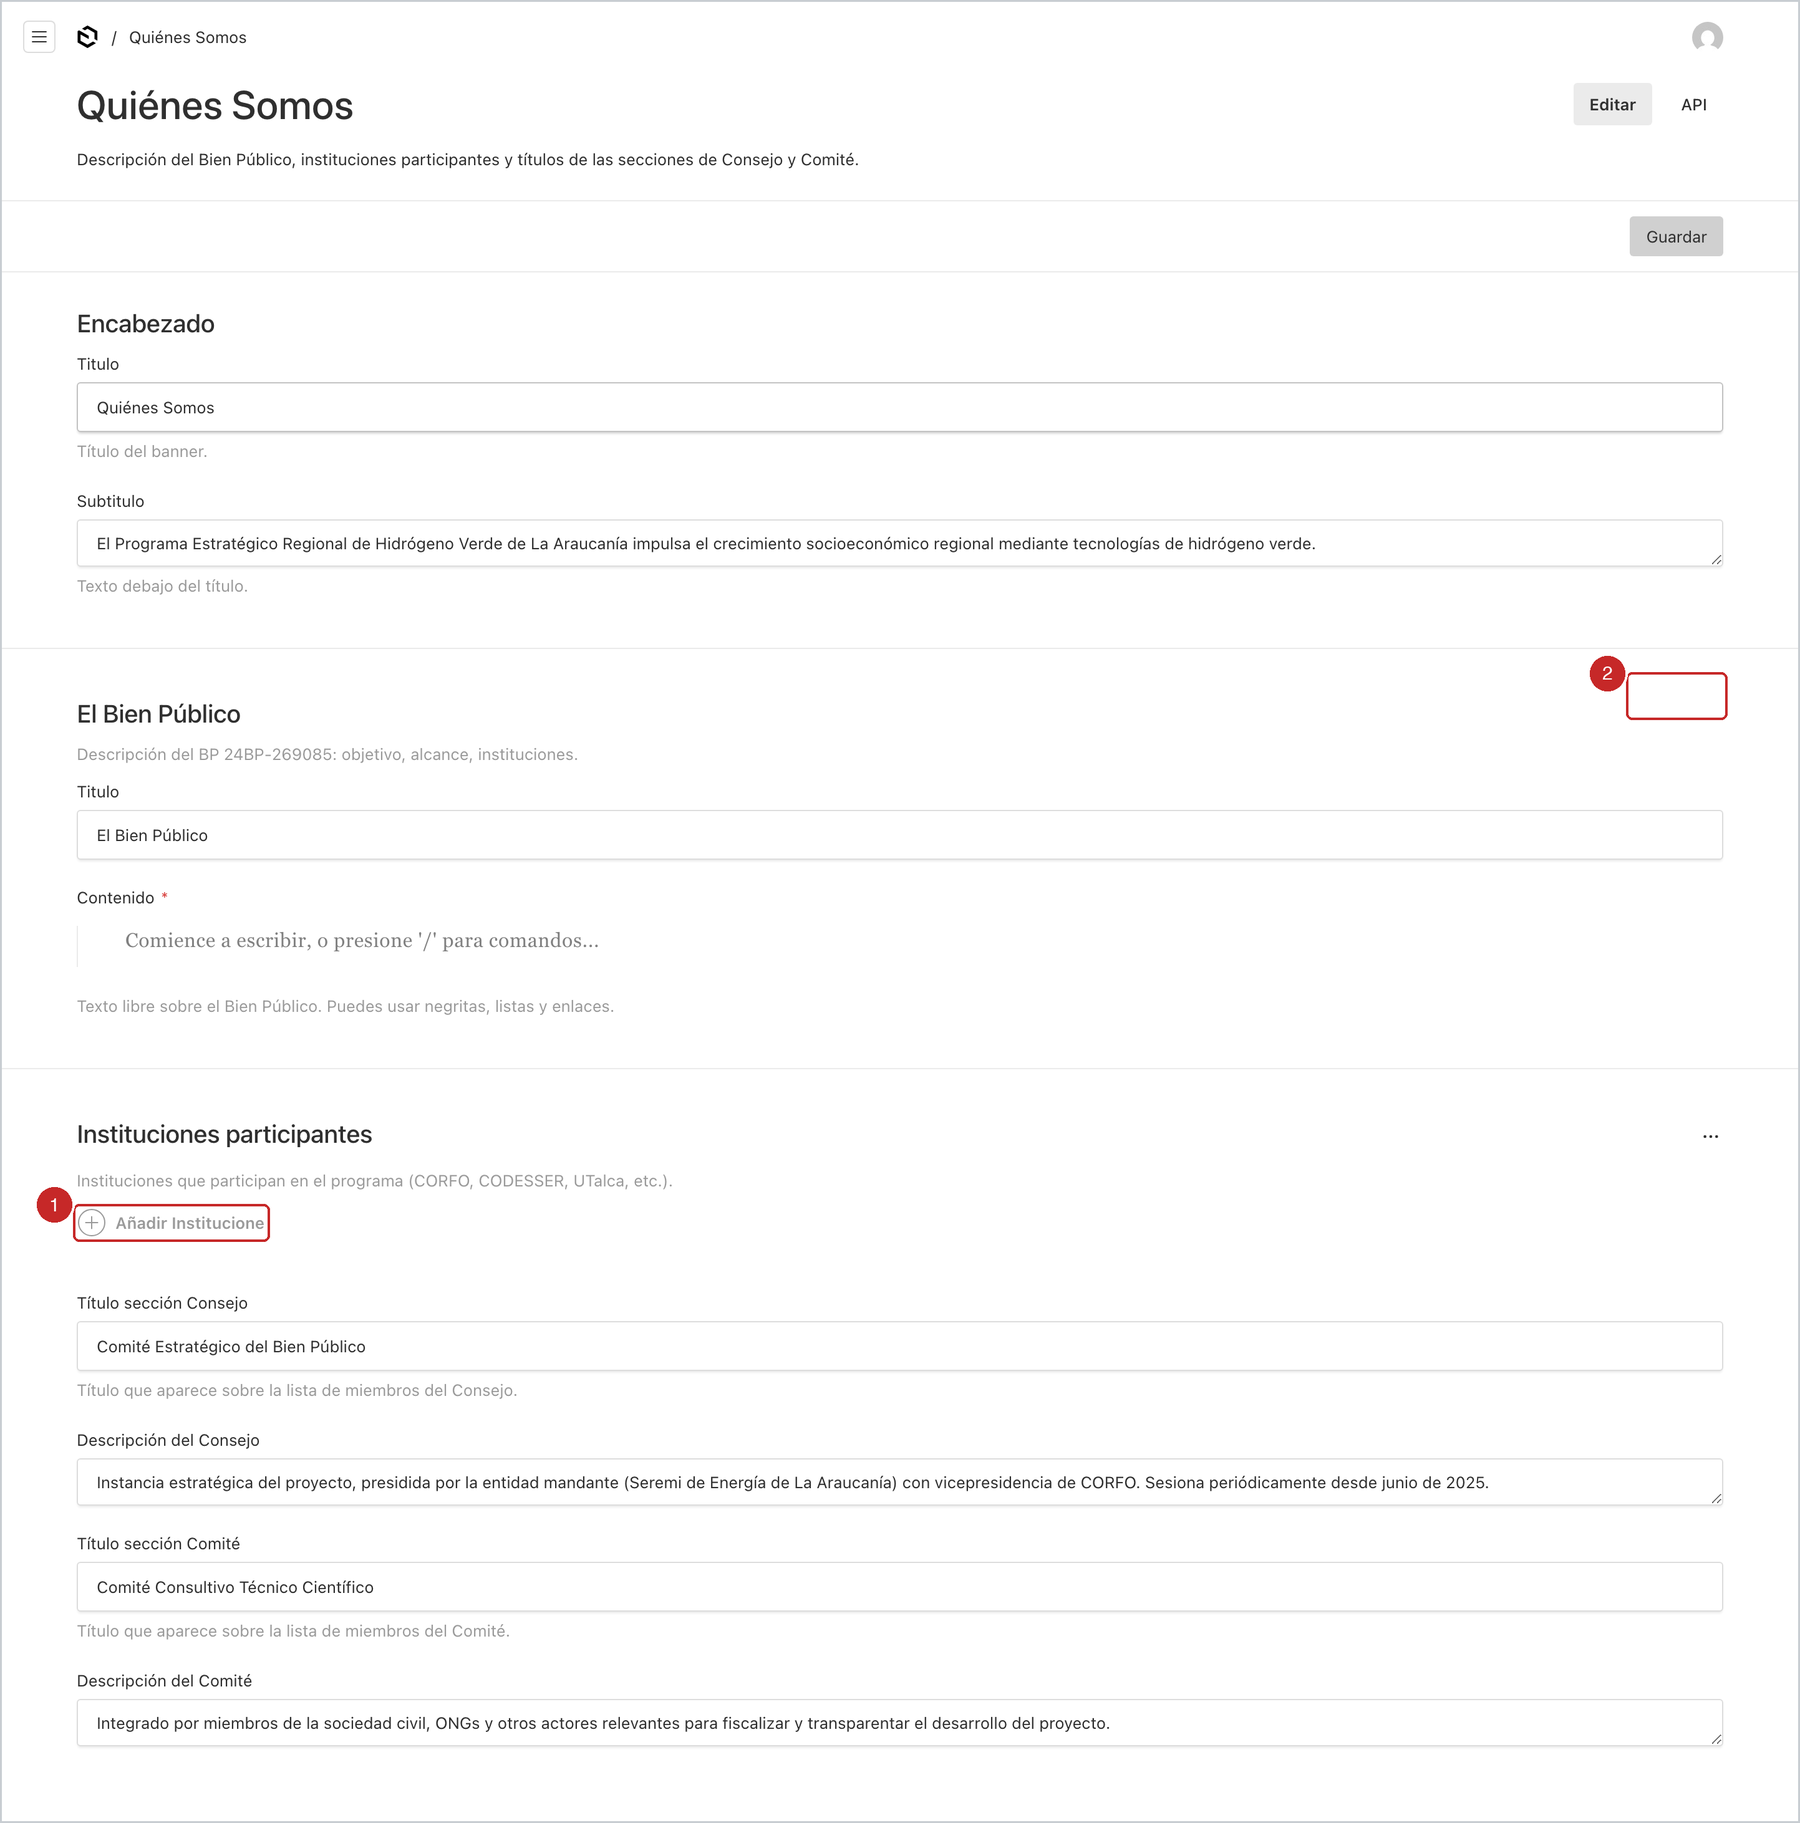
\includegraphics[width=\linewidth,keepaspectratio]{21-quienes-somos.png}
\caption{Formulario de Quiénes Somos.}
\end{figure}
\section{Gobernanza}
Menú lateral $\rightarrow$ \textbf{Páginas $\rightarrow$ Gobernanza}.

\begin{longtable}{>{\raggedright\arraybackslash}p{0.321\textwidth}>{\raggedright\arraybackslash}p{0.609\textwidth}}
\rowcolor{h2vazul}\textbf{\color{white}Sección} & \textbf{\color{white}Qué controla} \\
\endfirsthead
\rowcolor{h2vazul}\textbf{\color{white}Sección} & \textbf{\color{white}Qué controla} \\
\endhead
\textbf{Encabezado} y \textbf{Descripción general} & Banner y párrafo introductorio. \\ \midrule
\rowcolor{filaalt}\textbf{Nivel Estratégico} & Título, descripción, lista de \textbf{Funciones} (hasta 8) y periodicidad de reuniones del Consejo. \\ \midrule
\textbf{Nivel Operativo} & Lo mismo para la Unidad de Coordinación y Gestión. \\ \midrule
\rowcolor{filaalt}\textbf{Diagrama ''Estructura del Modelo''} & Los textos de las cajas del diagrama (consejo, comité, unidad) y los \textbf{Equipos} (cajas inferiores). \\ \midrule
\textbf{Evidencia de Actividades (galería de fotos)} & Las fotos con su descripción breve. \\ \bottomrule
\end{longtable}
\begin{figure}[H]\centering
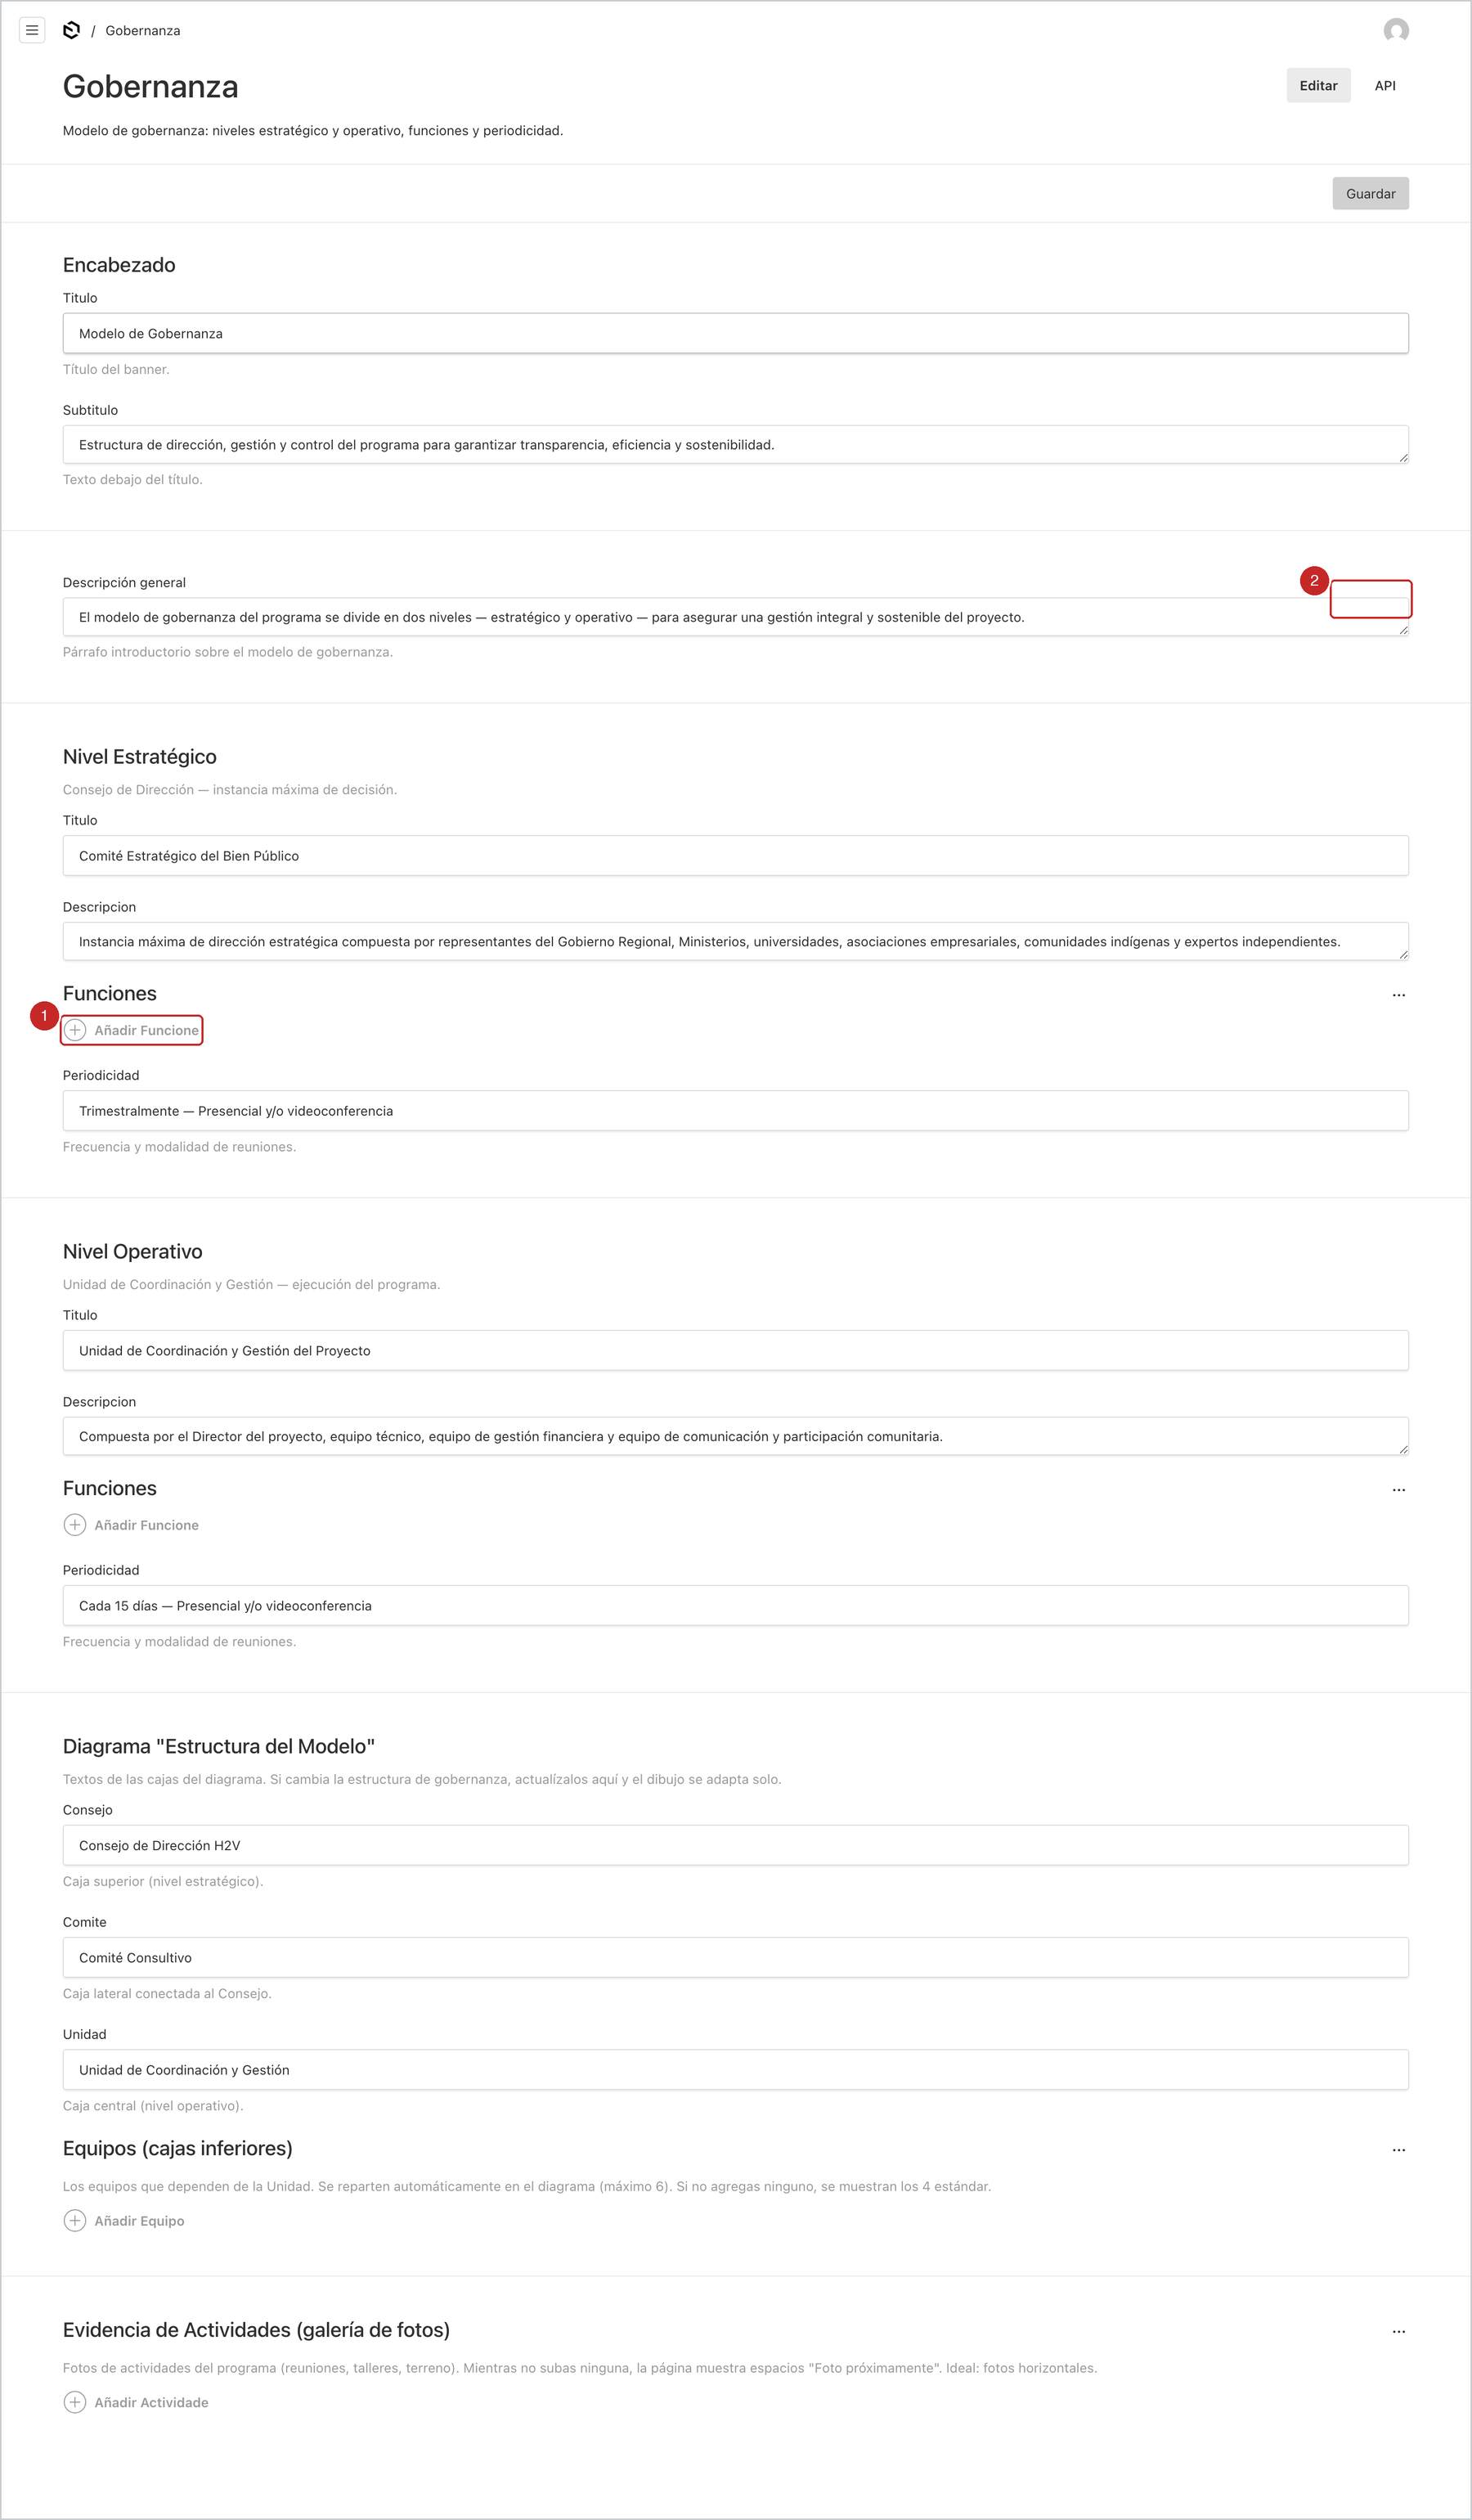
\includegraphics[width=\linewidth,height=0.74\textheight,keepaspectratio]{22-gobernanza.png}
\caption{Formulario de Gobernanza (vista completa).}
\end{figure}
\section{Contacto}
Menú lateral $\rightarrow$ \textbf{Configuración $\rightarrow$ Contacto} (solo Administradores). Tiene tres pestañas:

\begin{itemize}
  \item \textbf{Página}: título y bajada del encabezado, títulos de las columnas, etiquetas de los datos (correo, ubicación, teléfono, programa, ejecutores, mandante).
  \item \textbf{Formulario}: etiquetas y textos de ayuda de cada campo del formulario, las \textbf{Opciones de asunto} (lista editable), el texto del botón, y los mensajes de éxito y de error.
  \item \textbf{Datos institucionales}: \textbf{Email de contacto} (el que se muestra al público; también se actualiza solo en el pie de página, Privacidad y Accesibilidad), \textbf{Ubicación}, \textbf{Teléfono}, \textbf{Beneficiario (entidad ejecutora)}, \textbf{Coejecutor}, \textbf{Mandante} y \textbf{Código Bien Público}.
\end{itemize}
\begin{figure}[H]\centering
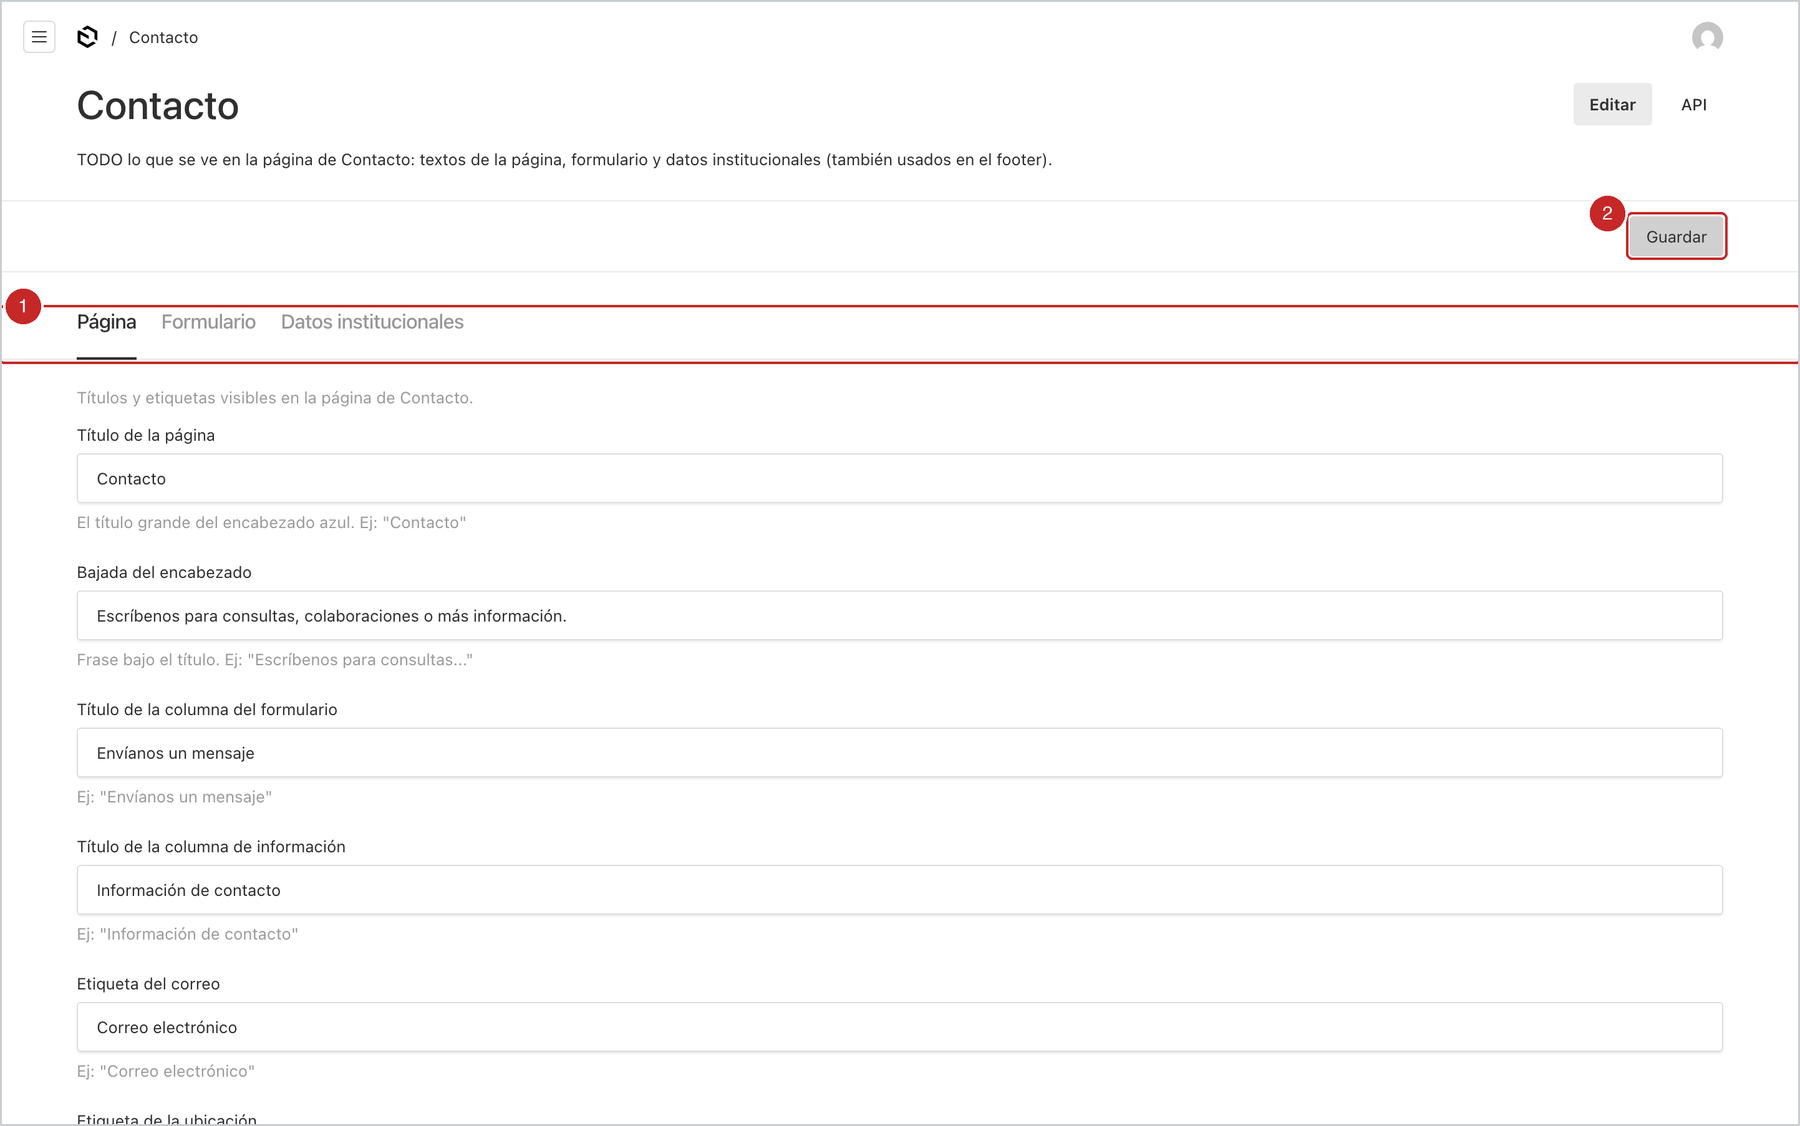
\includegraphics[width=\linewidth,keepaspectratio]{23-contacto-pagina.png}
\caption{Contacto, pestaña Página: las tres pestañas (1) y el botón Guardar (2).}
\end{figure}
\begin{figure}[H]\centering
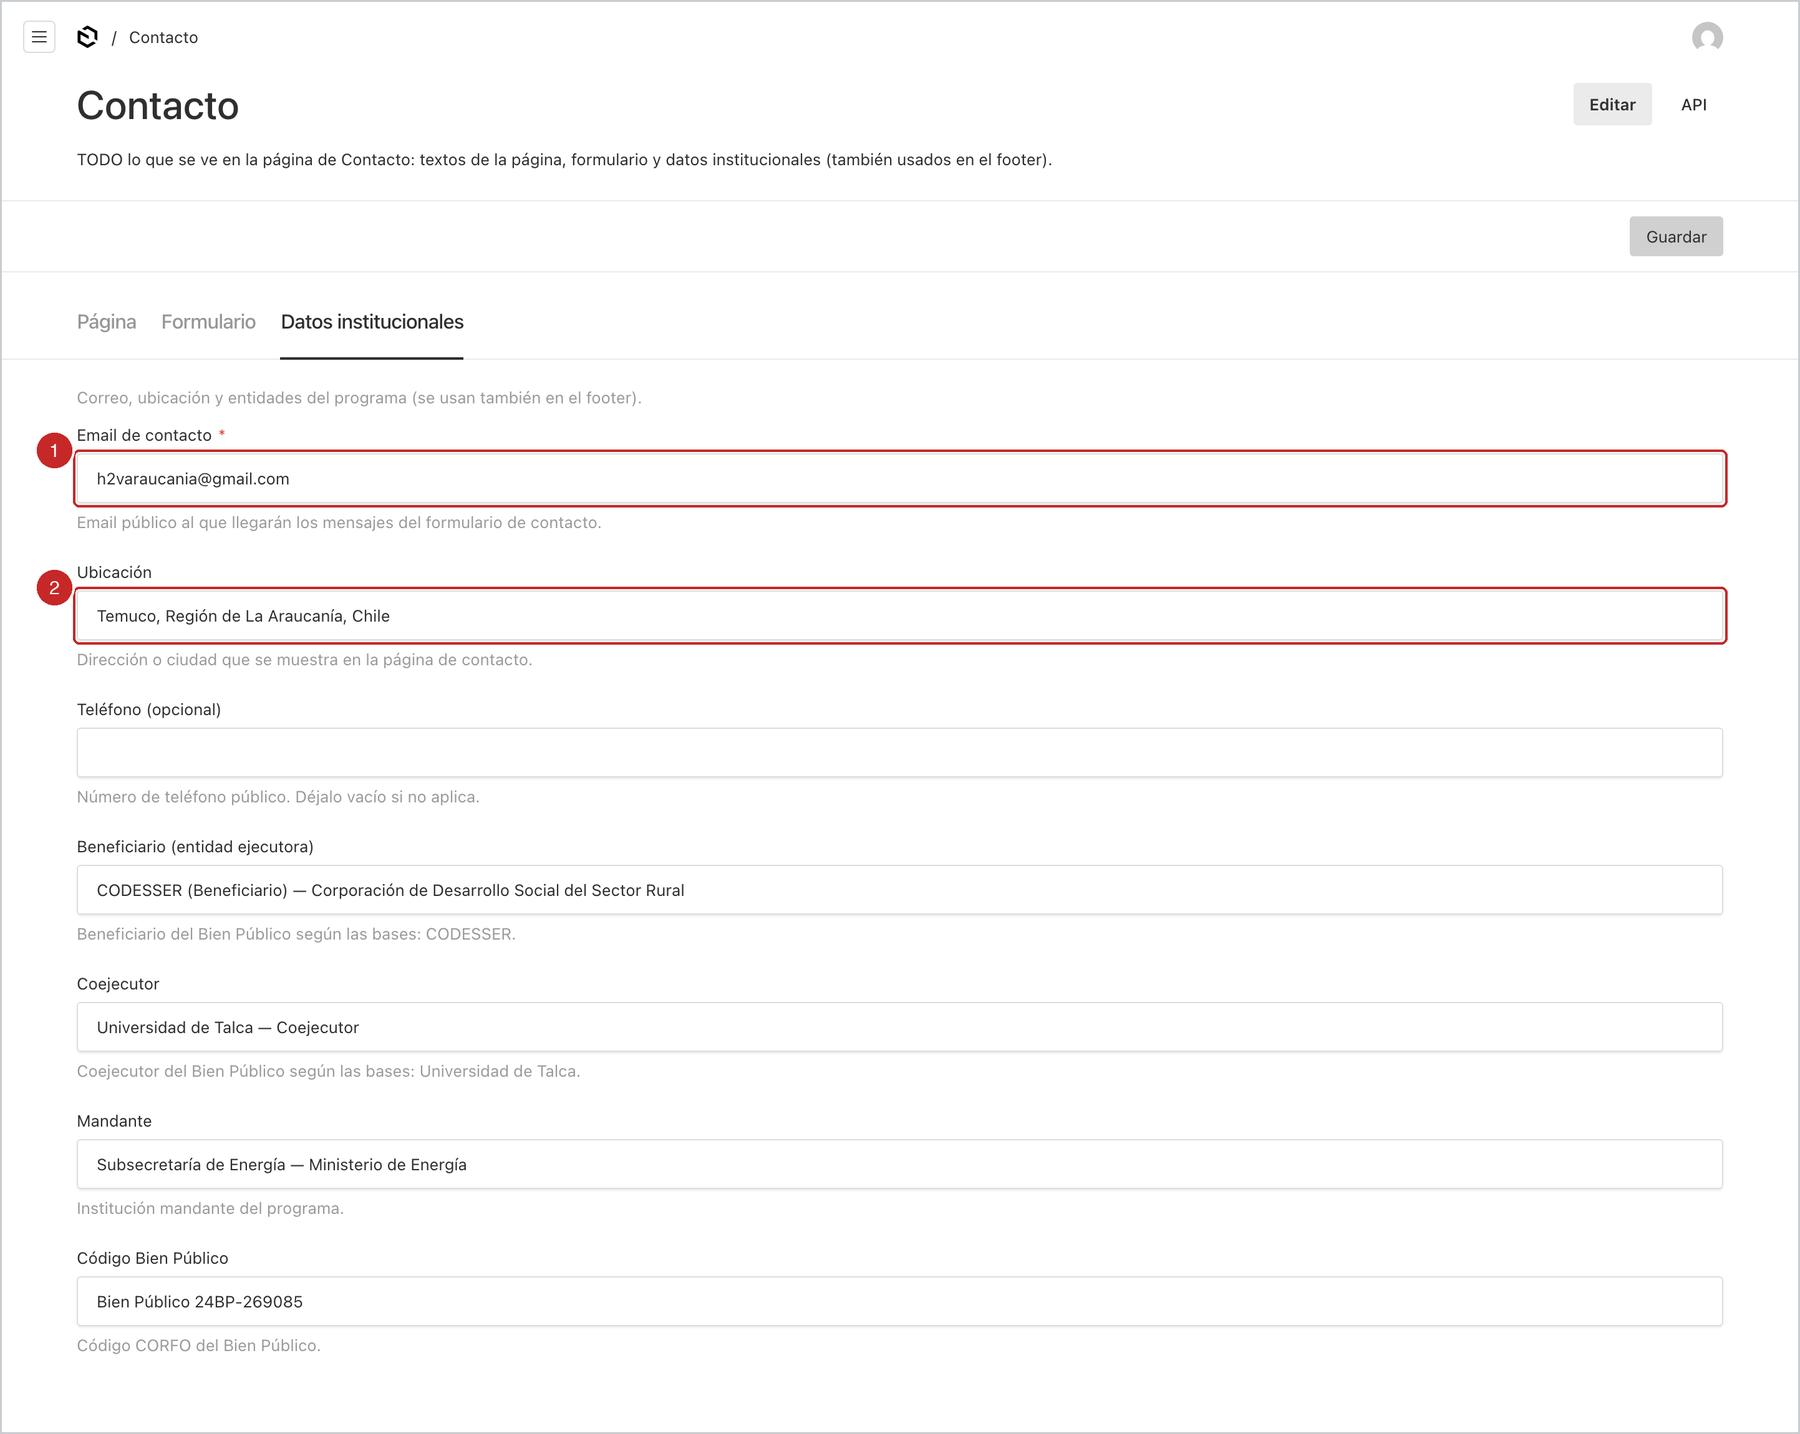
\includegraphics[width=\linewidth,keepaspectratio]{23b-contacto-datos.png}
\caption{Contacto, pestaña Datos institucionales: Email de contacto (1) y Ubicación (2).}
\end{figure}
\begin{figure}[H]\centering
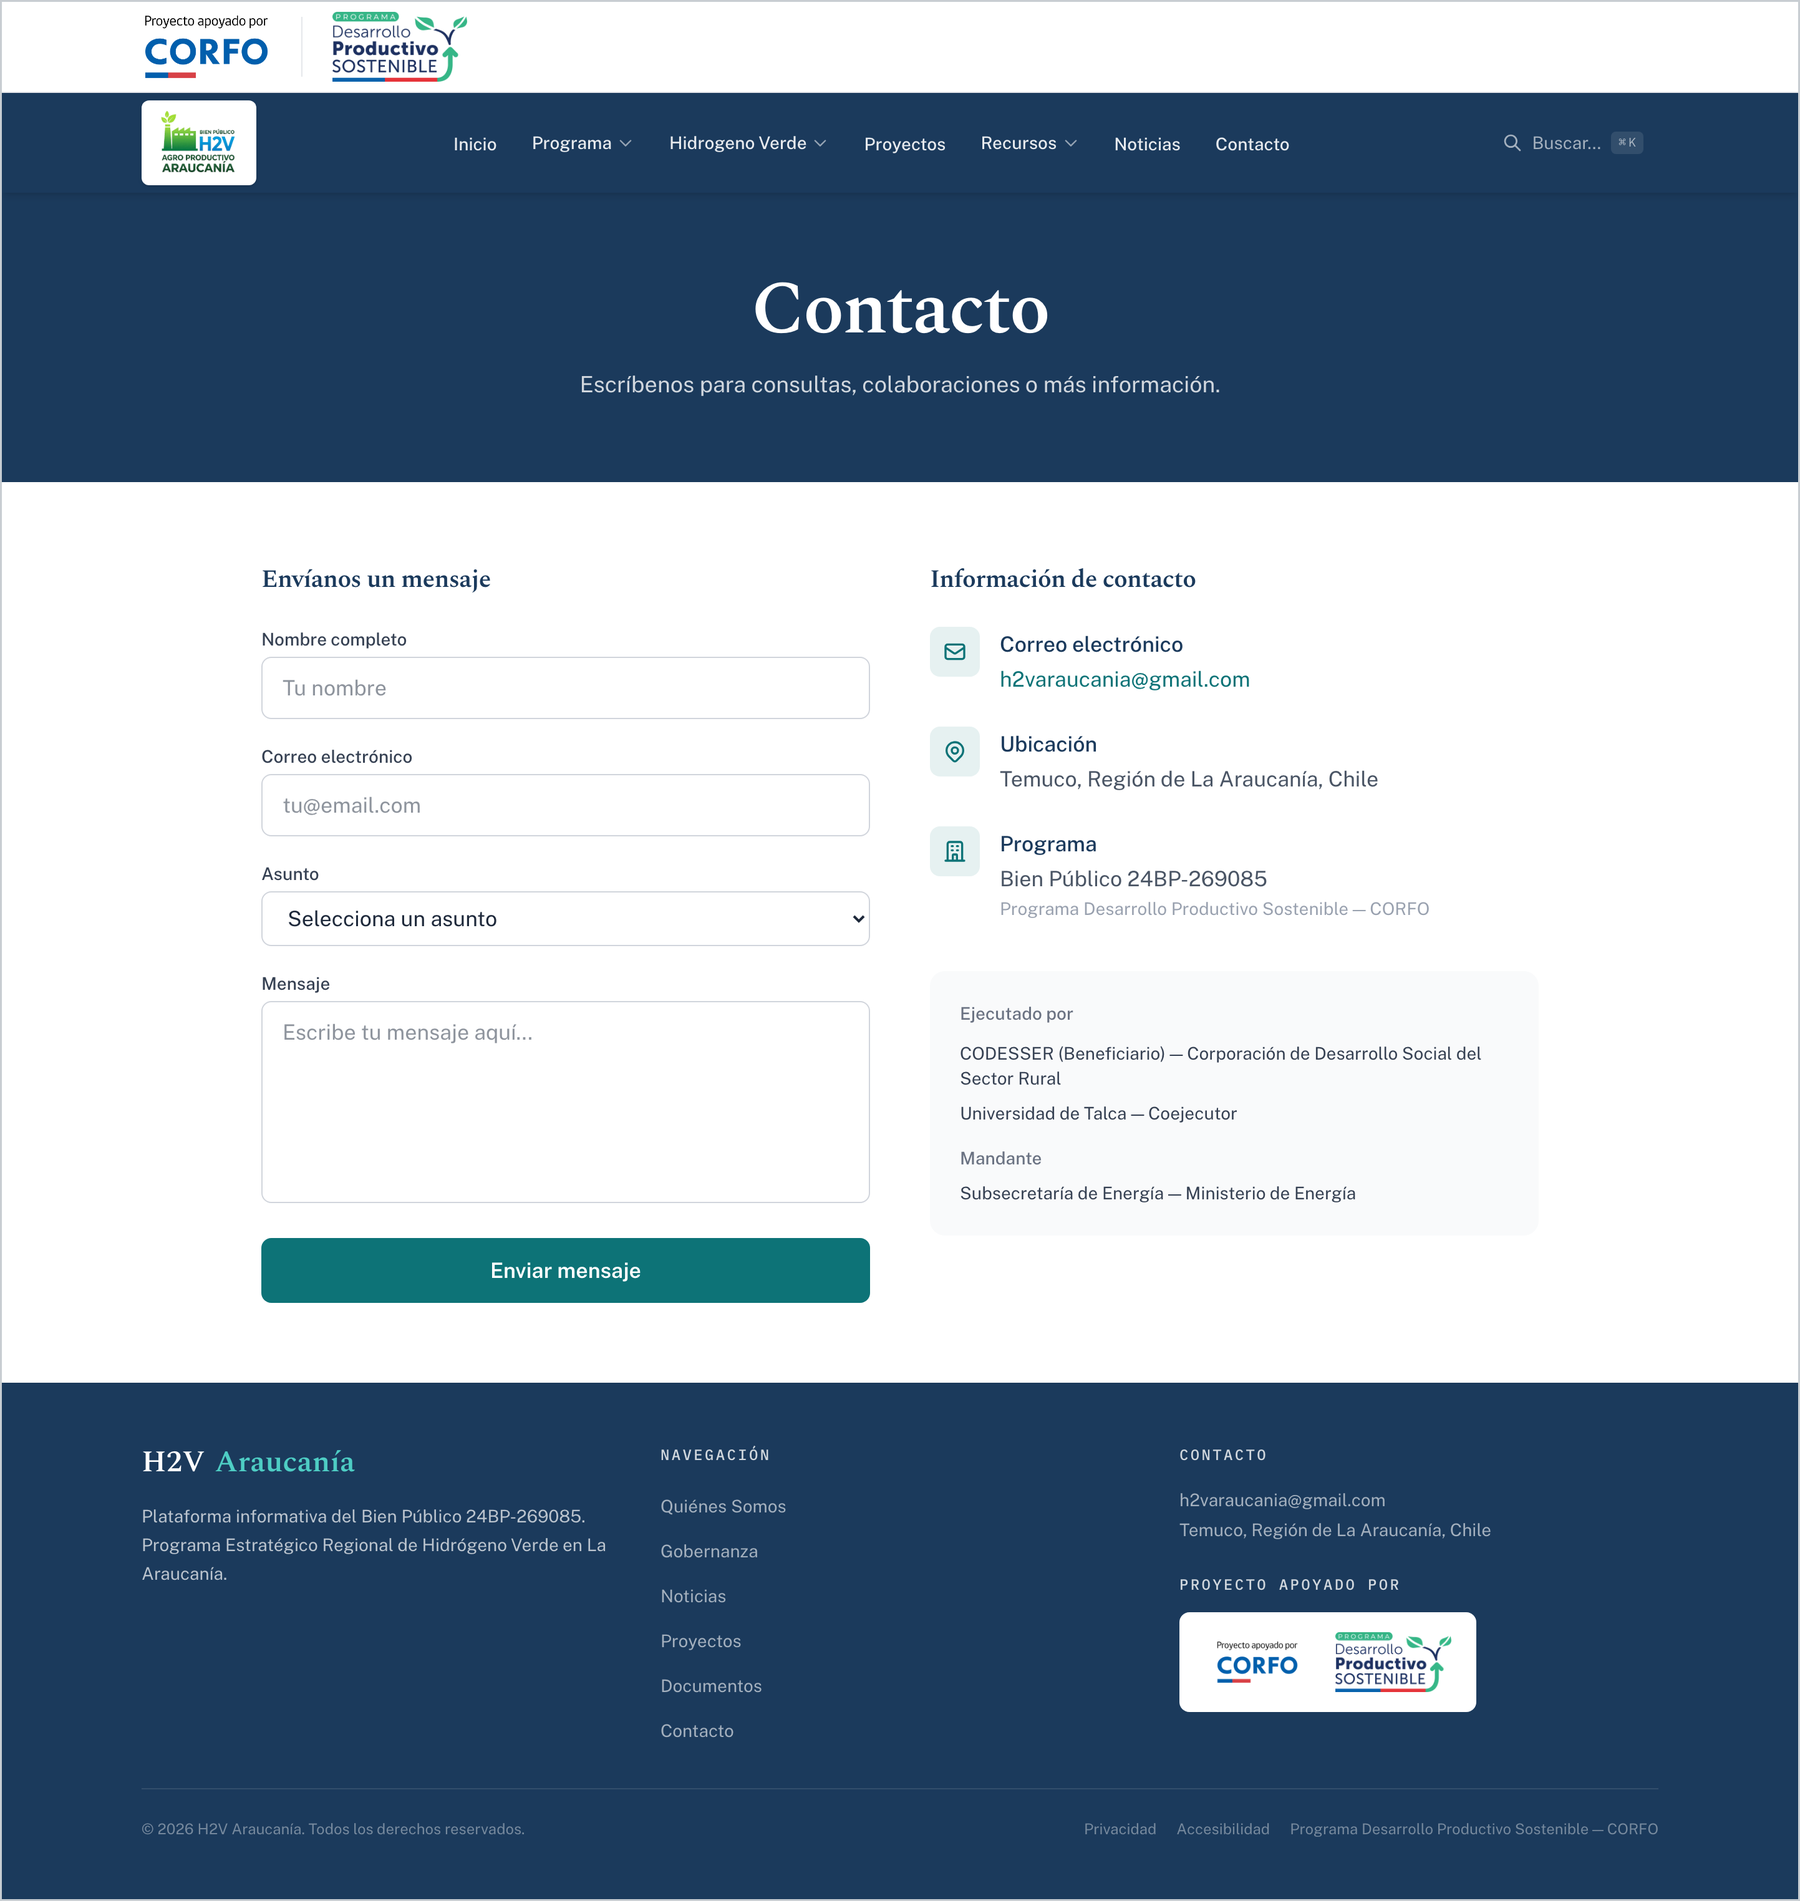
\includegraphics[width=\linewidth,keepaspectratio]{47-web-contacto.png}
\caption{Así se ve la página Contacto del sitio público.}
\end{figure}
\begin{recuadro}{cAtencion}{bAtencion}\textbf{\color{bAtencion}Atención:} el \textbf{Email de contacto} de esta pestaña es el que se \textbf{muestra} a los visitantes. La dirección a la que \textbf{llegan} los mensajes enviados por el formulario se configura en el servidor (variable \texttt{CONTACT\_\allowbreak{}EMAIL}); si cambia el correo institucional, pida al soporte técnico que actualice también esa variable (Anexo D).\end{recuadro}
\section{Configuración General}
Menú lateral $\rightarrow$ \textbf{Configuración $\rightarrow$ Configuración General} (solo Administradores).

\begin{longtable}{>{\raggedright\arraybackslash}p{0.366\textwidth}>{\raggedright\arraybackslash}p{0.564\textwidth}}
\rowcolor{h2vazul}\textbf{\color{white}Campo o sección} & \textbf{\color{white}Qué controla} \\
\endfirsthead
\rowcolor{h2vazul}\textbf{\color{white}Campo o sección} & \textbf{\color{white}Qué controla} \\
\endhead
\textbf{Nombre del sitio} & El nombre en la pestaña del navegador y en los resultados de Google. \\ \midrule
\rowcolor{filaalt}\textbf{Descripción SEO} & La frase que Google muestra bajo el nombre del sitio. Máximo 200 caracteres. \\ \midrule
\textbf{Texto del footer} y \textbf{Línea del programa (footer)} & Los textos de la primera columna del pie de página. \\ \midrule
\rowcolor{filaalt}\textbf{Título de la columna de navegación / de contacto (footer)}, \textbf{Leyenda de apoyo (footer)} & Los títulos pequeños en mayúsculas del pie de página. \\ \midrule
\textbf{Texto de derechos} & La línea ''© ... Todos los derechos reservados''. \\ \midrule
\rowcolor{filaalt}\textbf{Título, Texto, Botón principal y Botón secundario de la página 404} & La página que ve un visitante cuando escribe una dirección que no existe. \\ \midrule
\textbf{Logos institucionales} & La lista de instituciones participantes (nombre y logo) que se muestra en la portada y en el pie de página. \\ \bottomrule
\end{longtable}
\begin{figure}[H]\centering
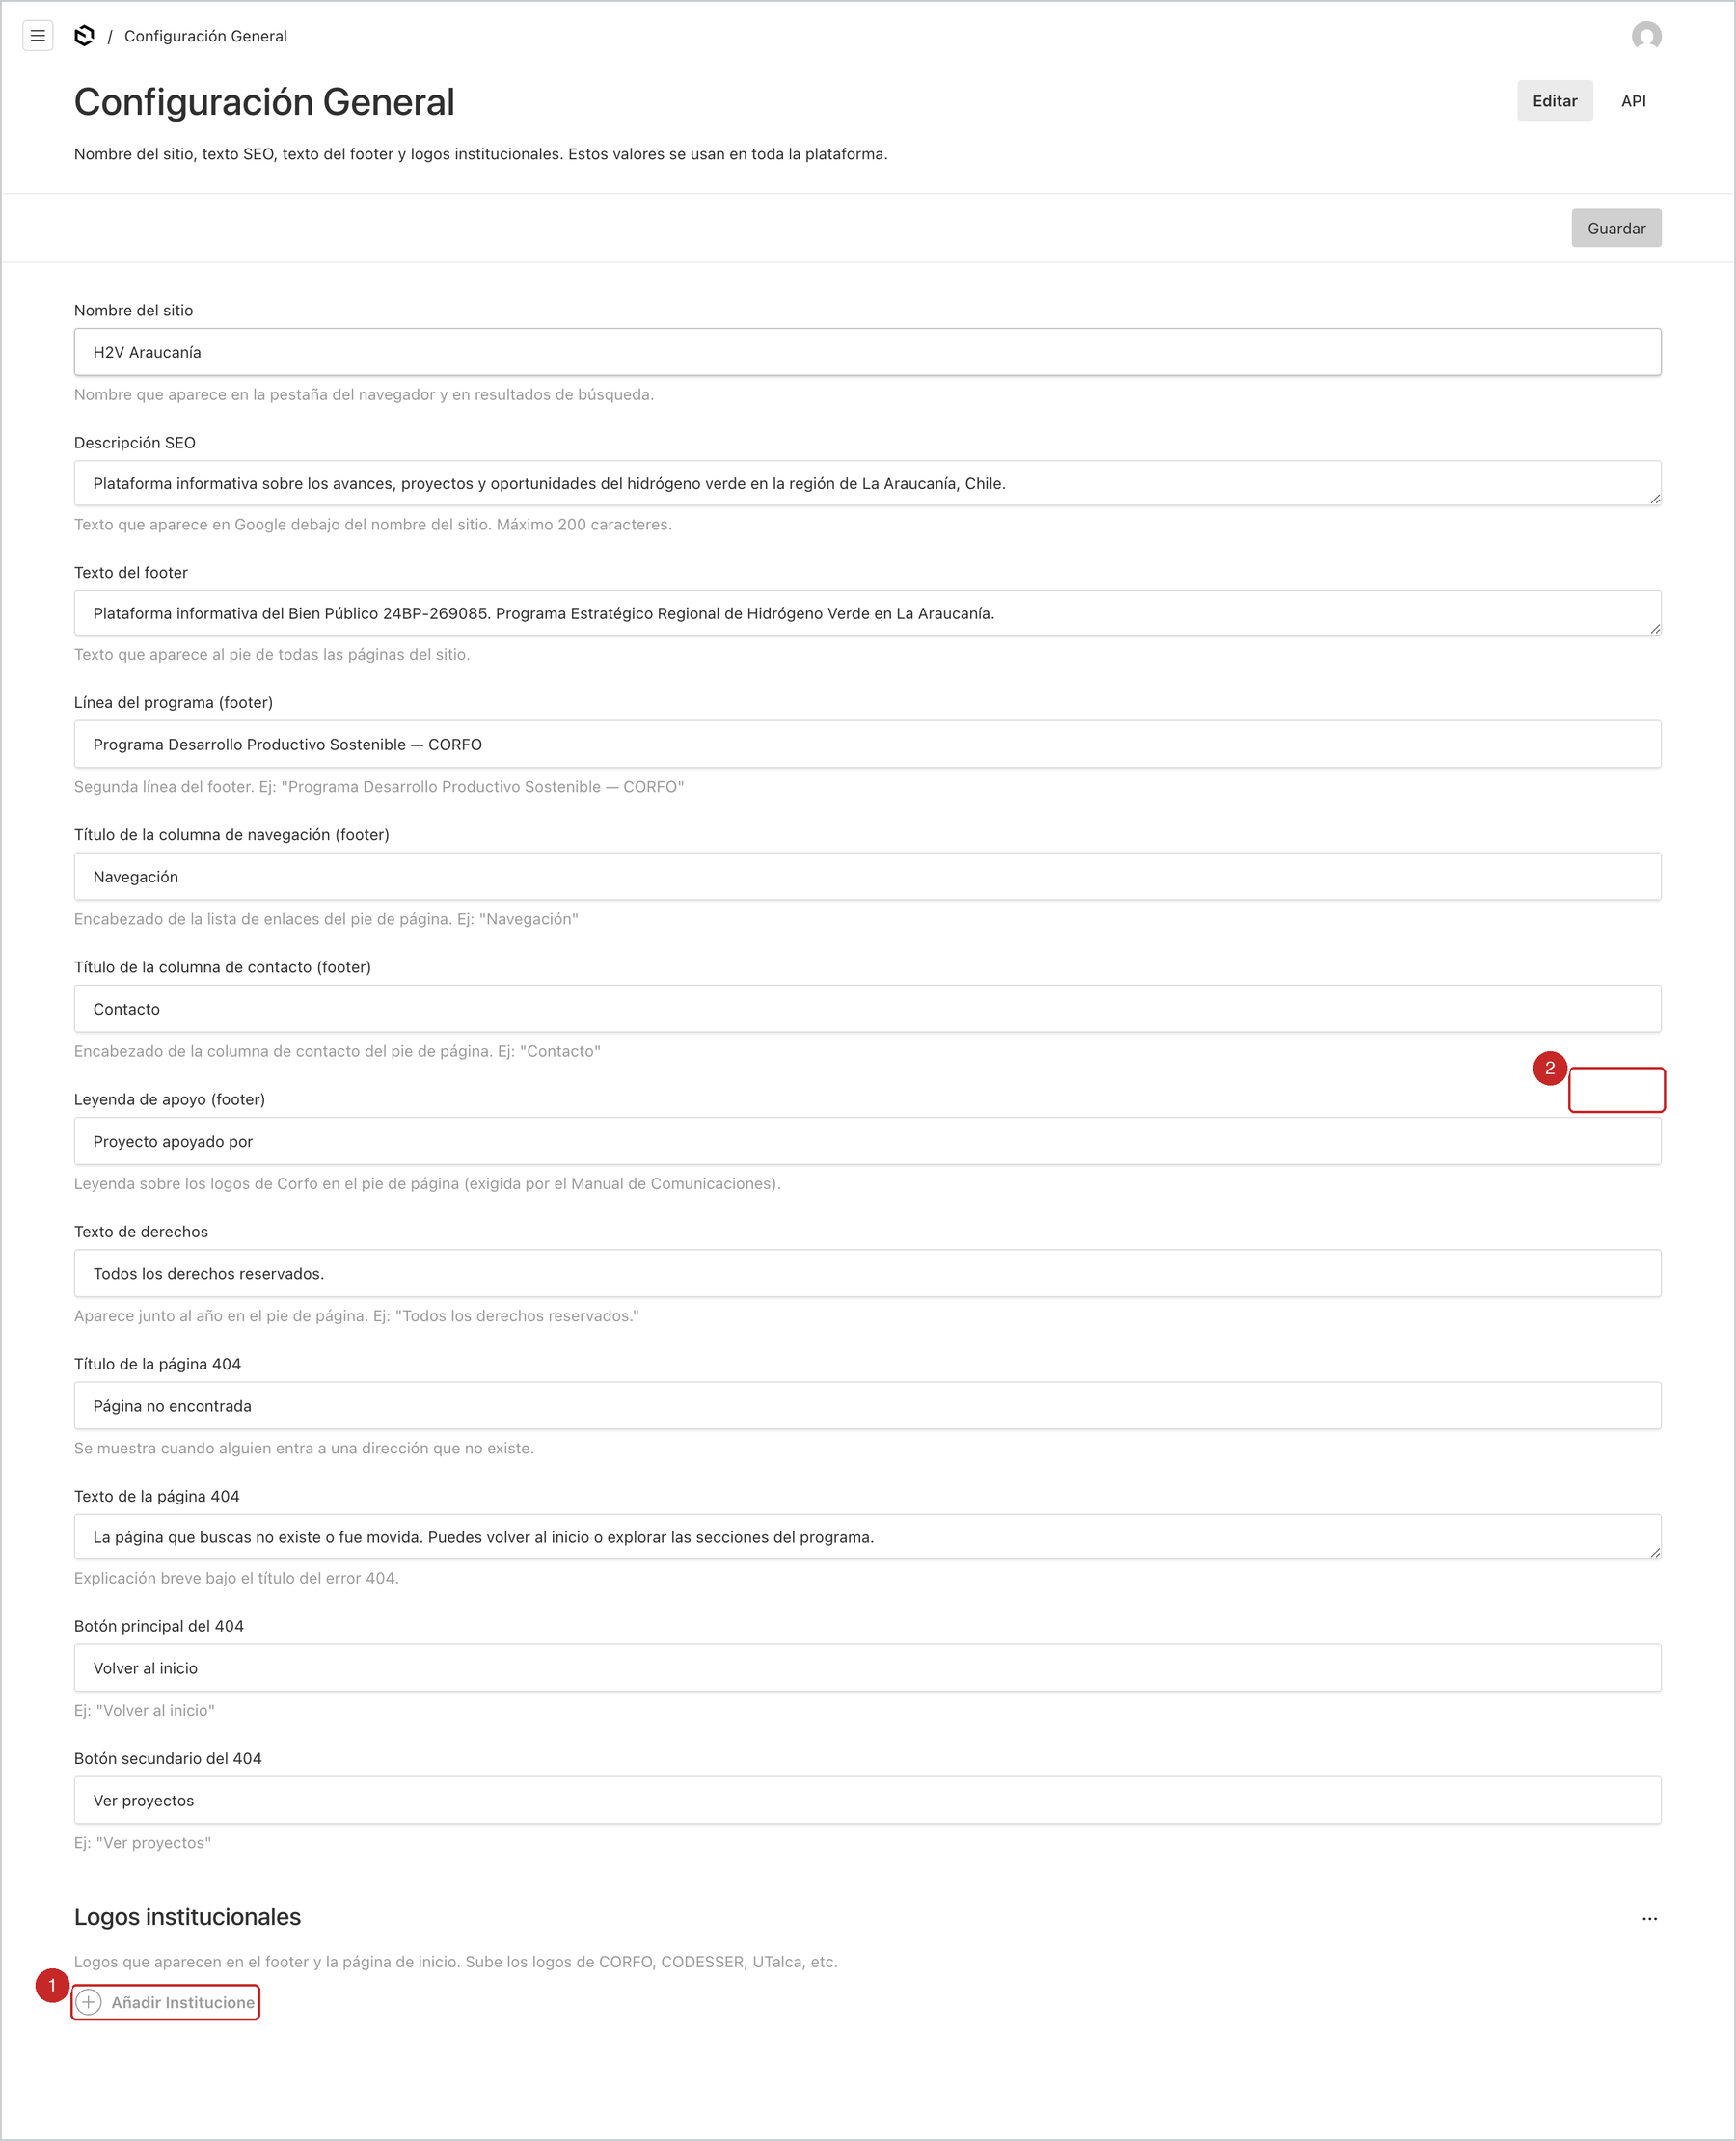
\includegraphics[width=\linewidth,keepaspectratio]{24-sitio-general.png}
\caption{Formulario de Configuración General.}
\end{figure}
\section{Las demás páginas}
Todas se editan igual (Páginas $\rightarrow$ nombre de la página $\rightarrow$ Guardar). Resumen de lo que contiene cada una:

\begin{longtable}{>{\raggedright\arraybackslash}p{0.187\textwidth}>{\raggedright\arraybackslash}p{0.743\textwidth}}
\rowcolor{h2vazul}\textbf{\color{white}Página} & \textbf{\color{white}Qué se puede editar} \\
\endfirsthead
\rowcolor{h2vazul}\textbf{\color{white}Página} & \textbf{\color{white}Qué se puede editar} \\
\endhead
\textbf{Hidrógeno Verde} & Encabezado; ''¿Qué es el H2V?'' (texto libre); Proceso de Electrólisis (pasos); Tipos de Electrolizadores (nombre, madurez, costo); Cadena de Valor (ítems con emoji e ícono); Derivados del H2V (aplicación principal); Sección ''Explora más'' (tarjetas con página de destino). \\ \midrule
\rowcolor{filaalt}\textbf{Sectores Productivos} & Encabezado; lista de Sectores, cada uno con emoji, descripción y sus Oportunidades. \\ \midrule
\textbf{Hoja de Ruta} & Encabezado; Hitos del timeline (Año/Período, título, descripción); Nota al pie. \\ \midrule
\rowcolor{filaalt}\textbf{Capital Humano} & Encabezado; texto introductorio; Perfiles laborales emergentes; Programas de formación del BP; Nota de oportunidad regional. \\ \midrule
\textbf{Marco Regulatorio} & Encabezado; Documentos normativos (nombre, descripción, relevancia para La Araucanía, enlace). \\ \midrule
\rowcolor{filaalt}\textbf{Comunidad} & Encabezado; texto introductorio; Participación en gobernanza; Compromiso con el territorio; Glosario Mapudungún (término y significado). \\ \midrule
\textbf{Transparencia} & Encabezado; texto introductorio; Secciones de transparencia (título y descripción de cada bloque). \\ \midrule
\rowcolor{filaalt}\textbf{Mediateca} & Encabezado; Recursos multimedia (tipo: video, infografía, presentación o documento; título; enlace); mensaje cuando no hay recursos. \\ \midrule
\textbf{Mapa de Proyectos} & Título y subtítulo del encabezado de la página del mapa (los puntos vienen de Contenido $\rightarrow$ Proyectos). \\ \midrule
\rowcolor{filaalt}\textbf{Política de Privacidad} & Encabezado, fecha de última actualización y texto completo (opcional; si se deja vacío se usa el texto estándar). \\ \midrule
\textbf{Accesibilidad} & Encabezado y texto completo de la declaración (opcional). \\ \bottomrule
\end{longtable}
\begin{figure}[H]\centering
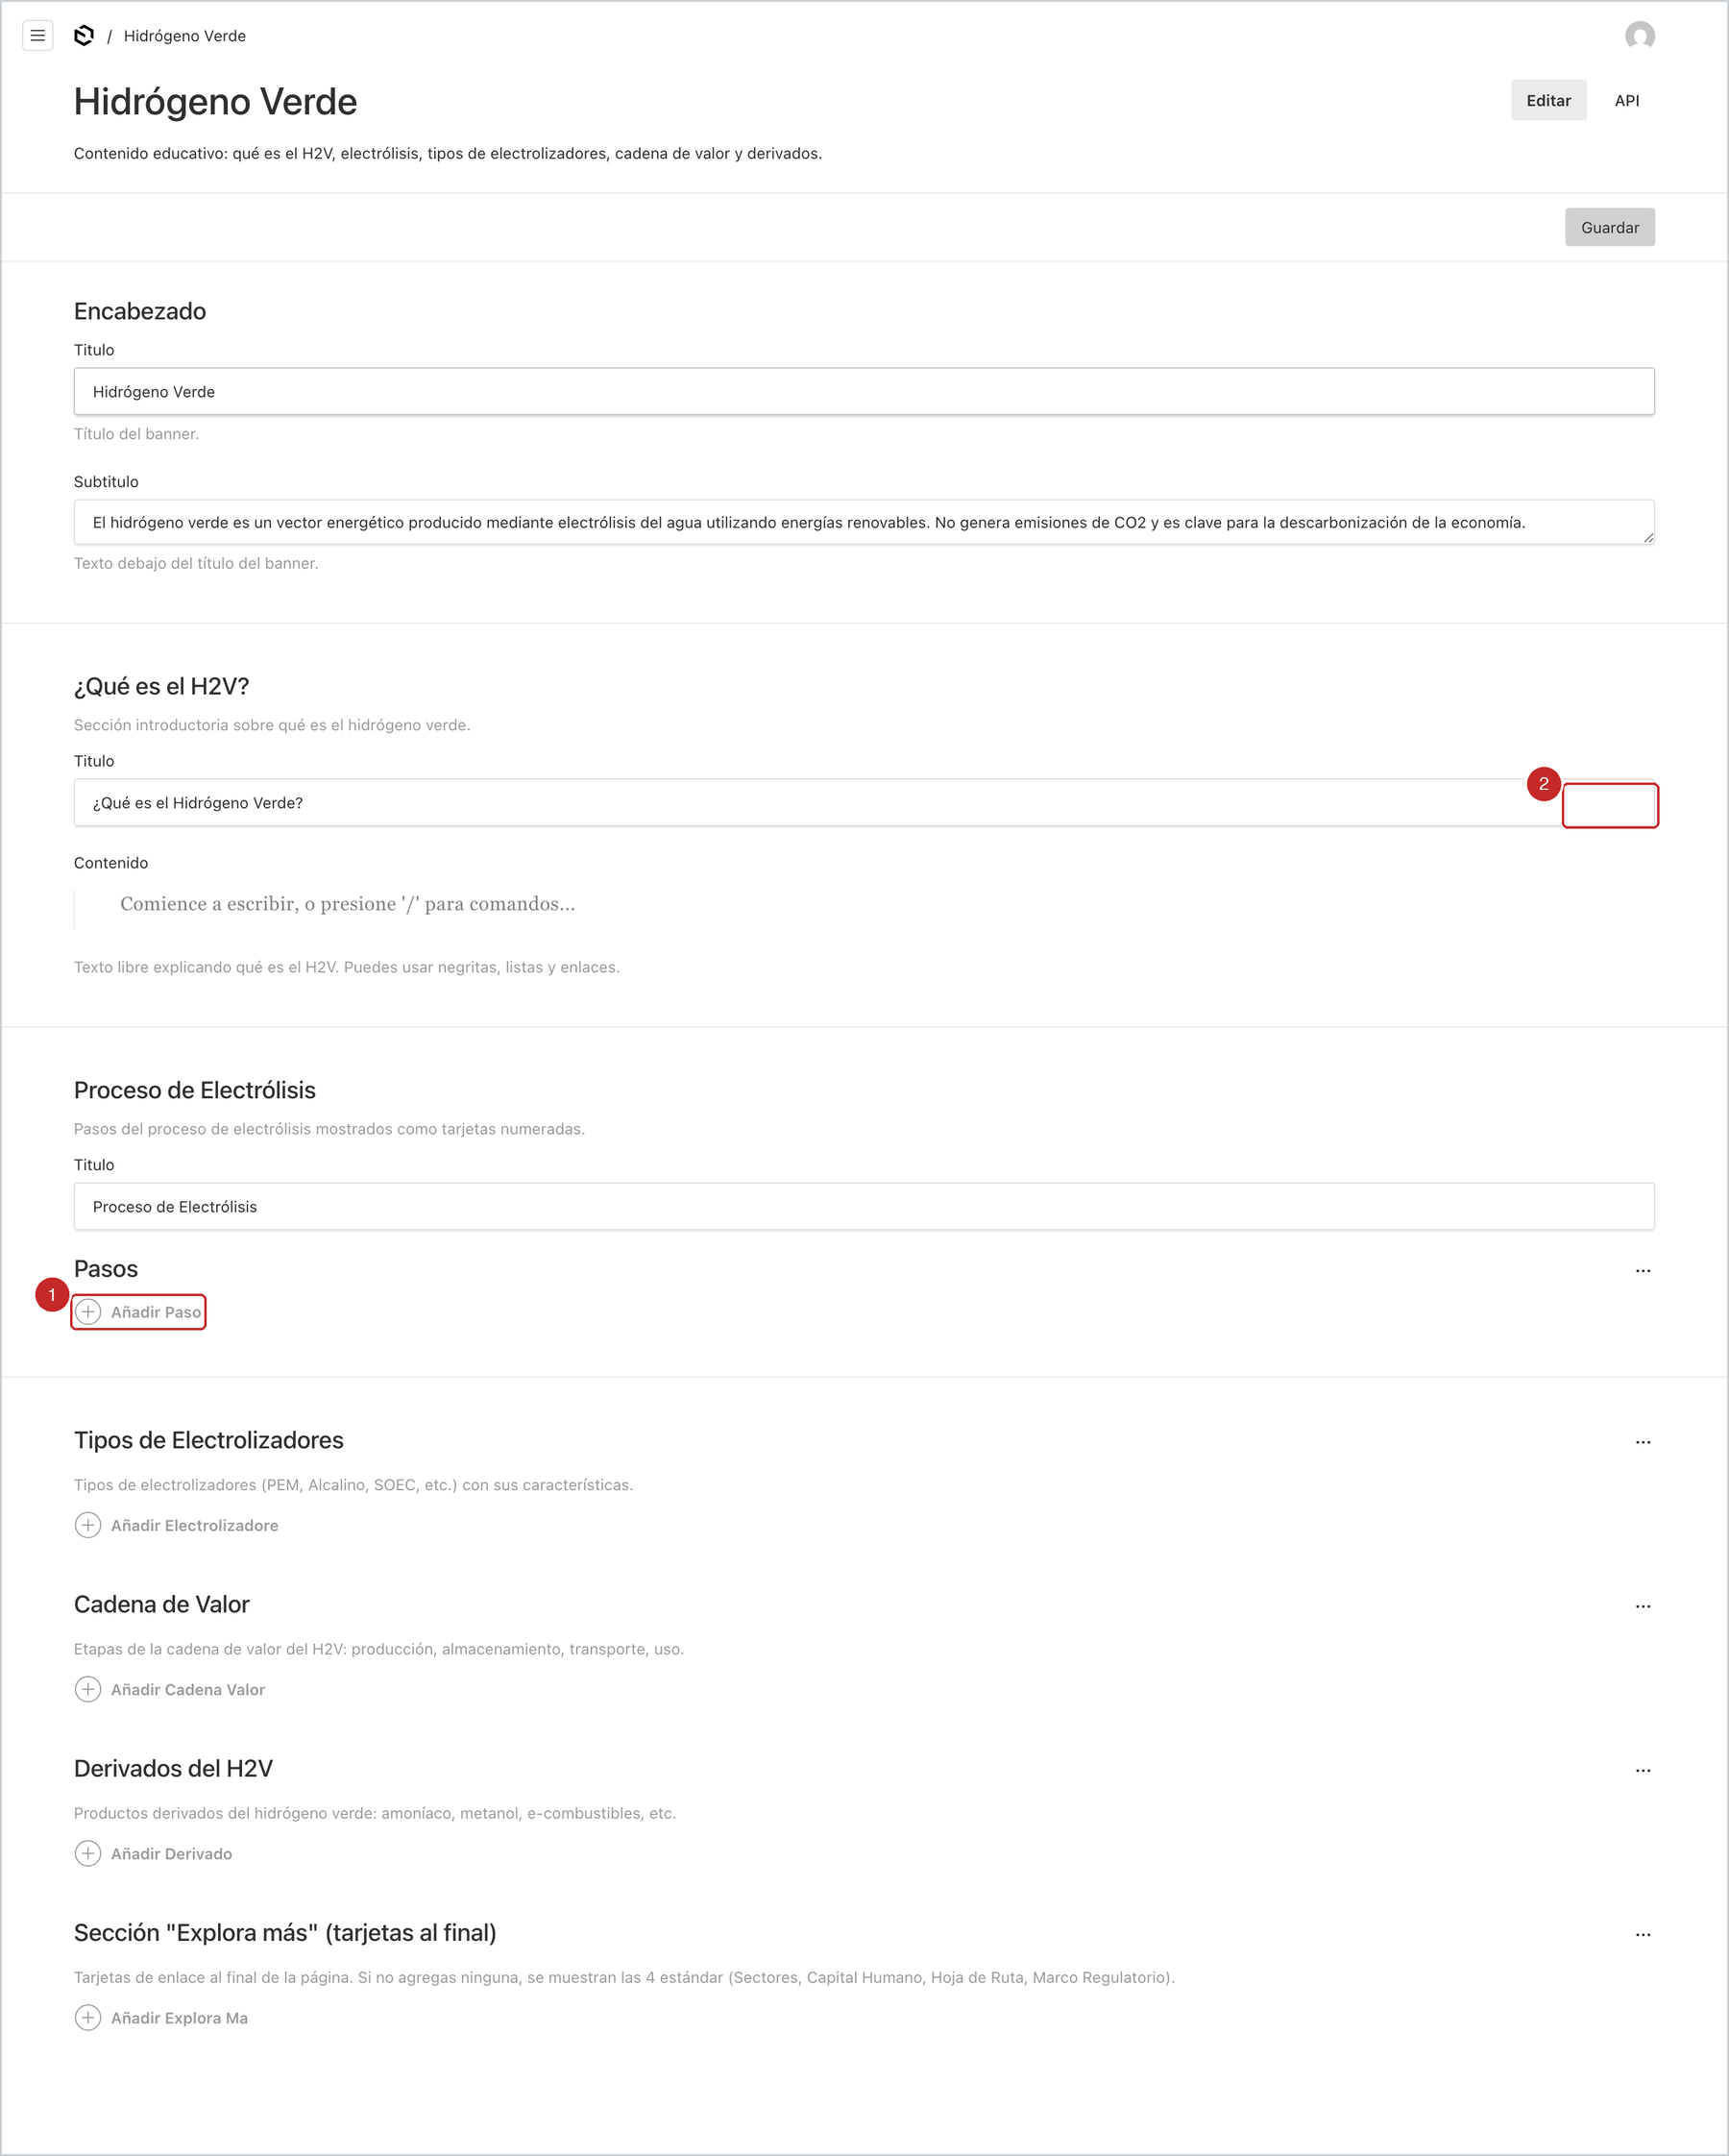
\includegraphics[width=\linewidth,keepaspectratio]{26-hidrogeno-verde.png}
\caption{Formulario de Hidrógeno Verde (vista completa).}
\end{figure}
\begin{figure}[H]\centering
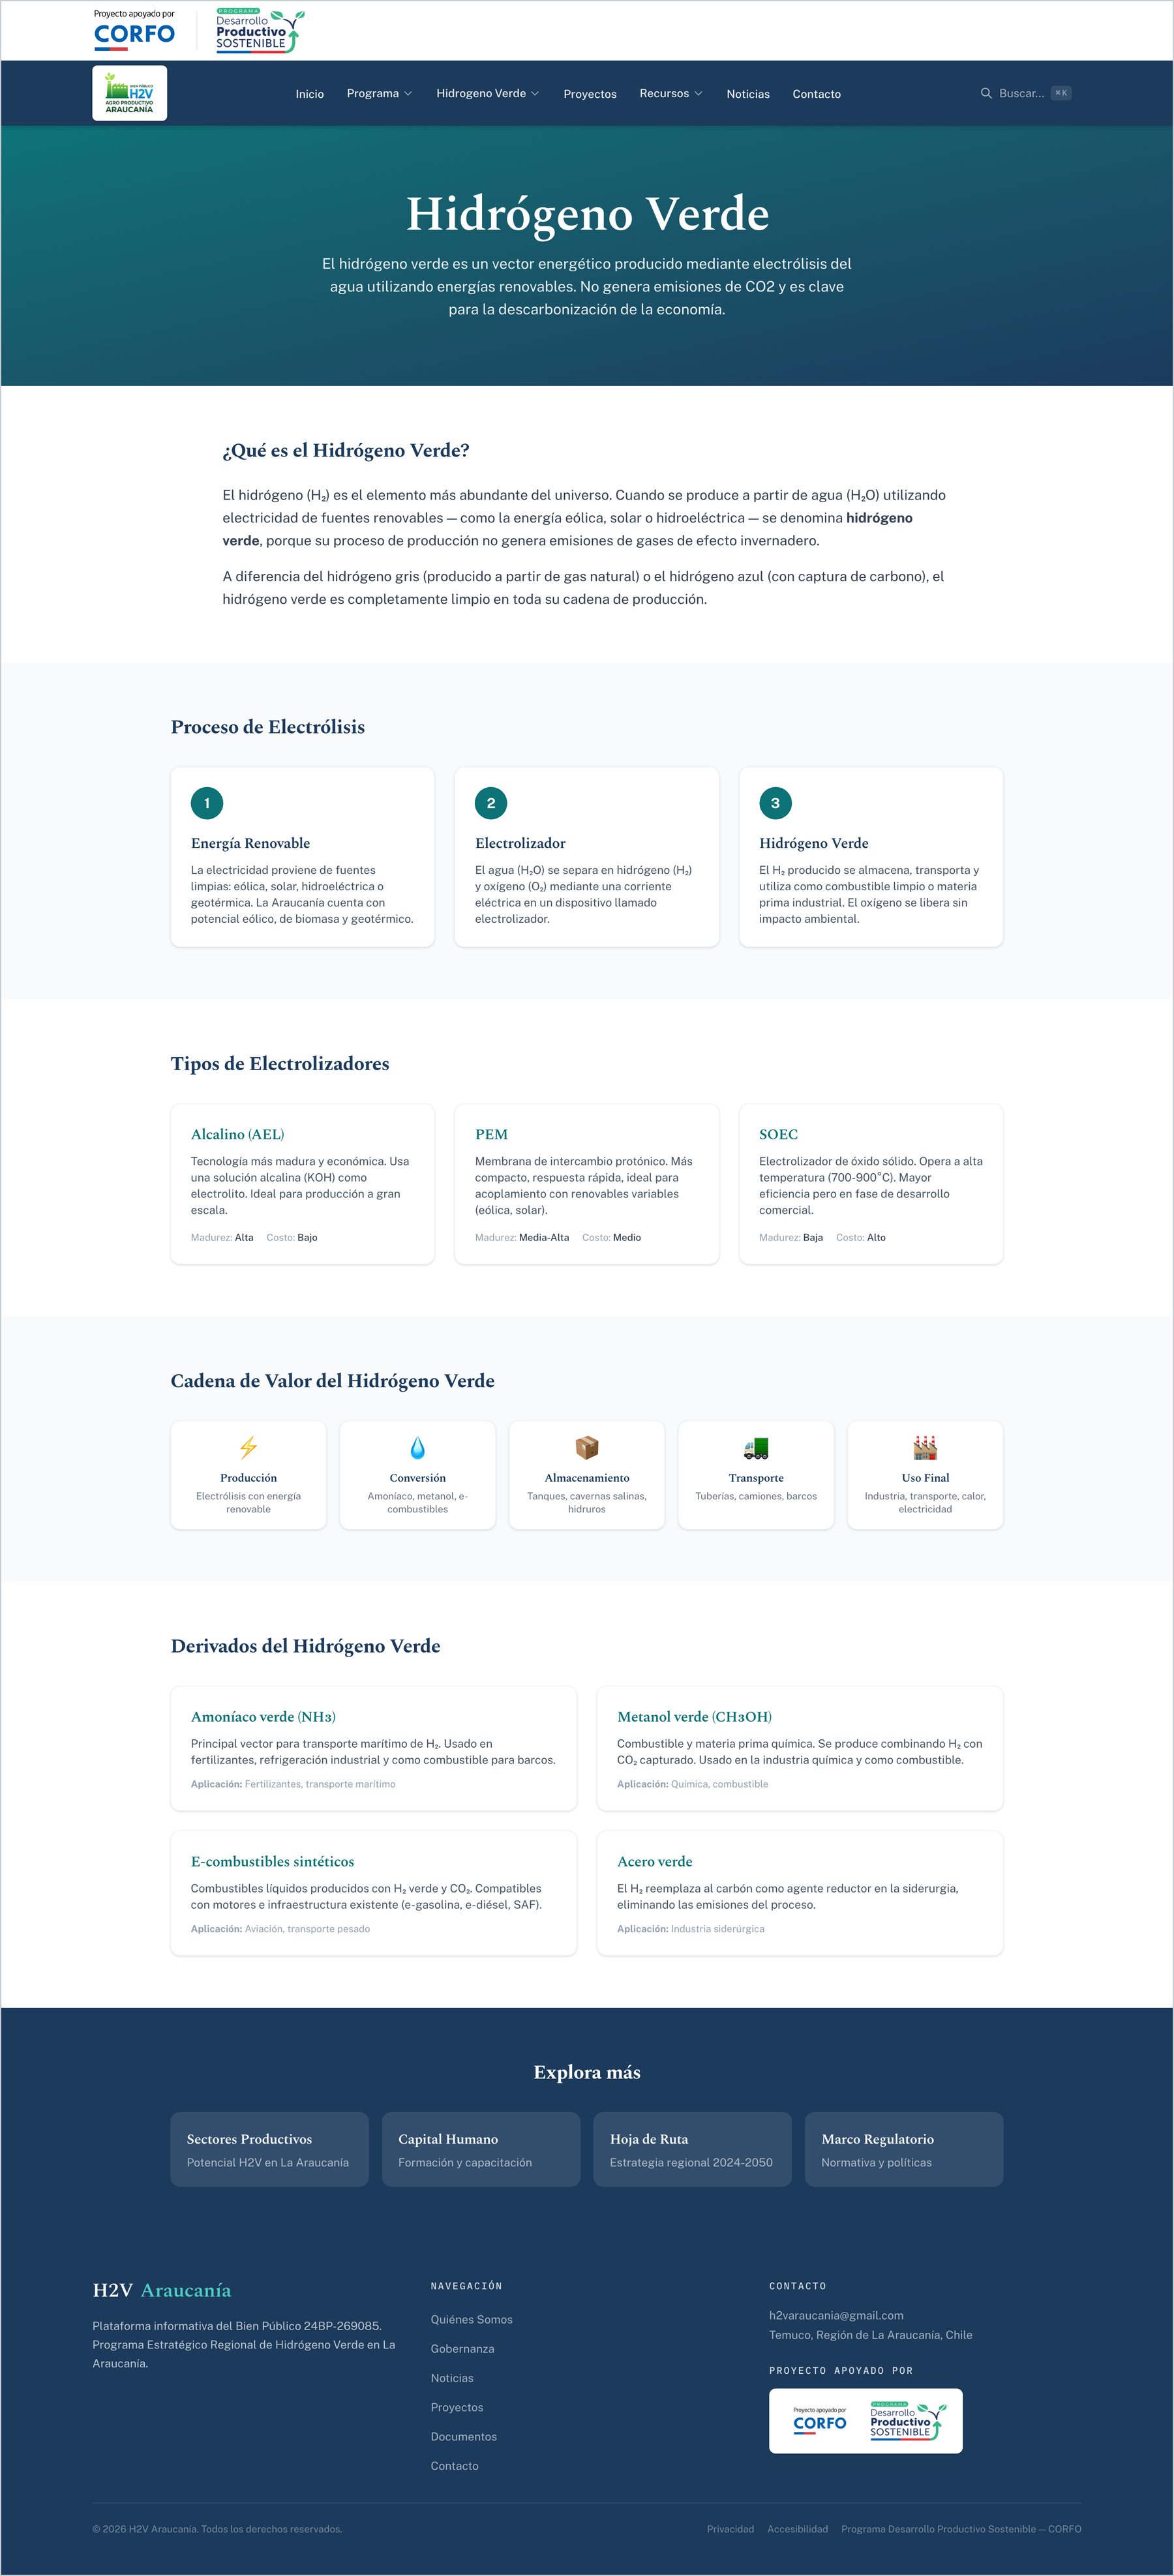
\includegraphics[width=\linewidth,height=0.74\textheight,keepaspectratio]{49-web-hidrogeno-verde.png}
\caption{Así se ve la página Hidrógeno Verde del sitio público.}
\end{figure}
\begin{figure}[H]\centering
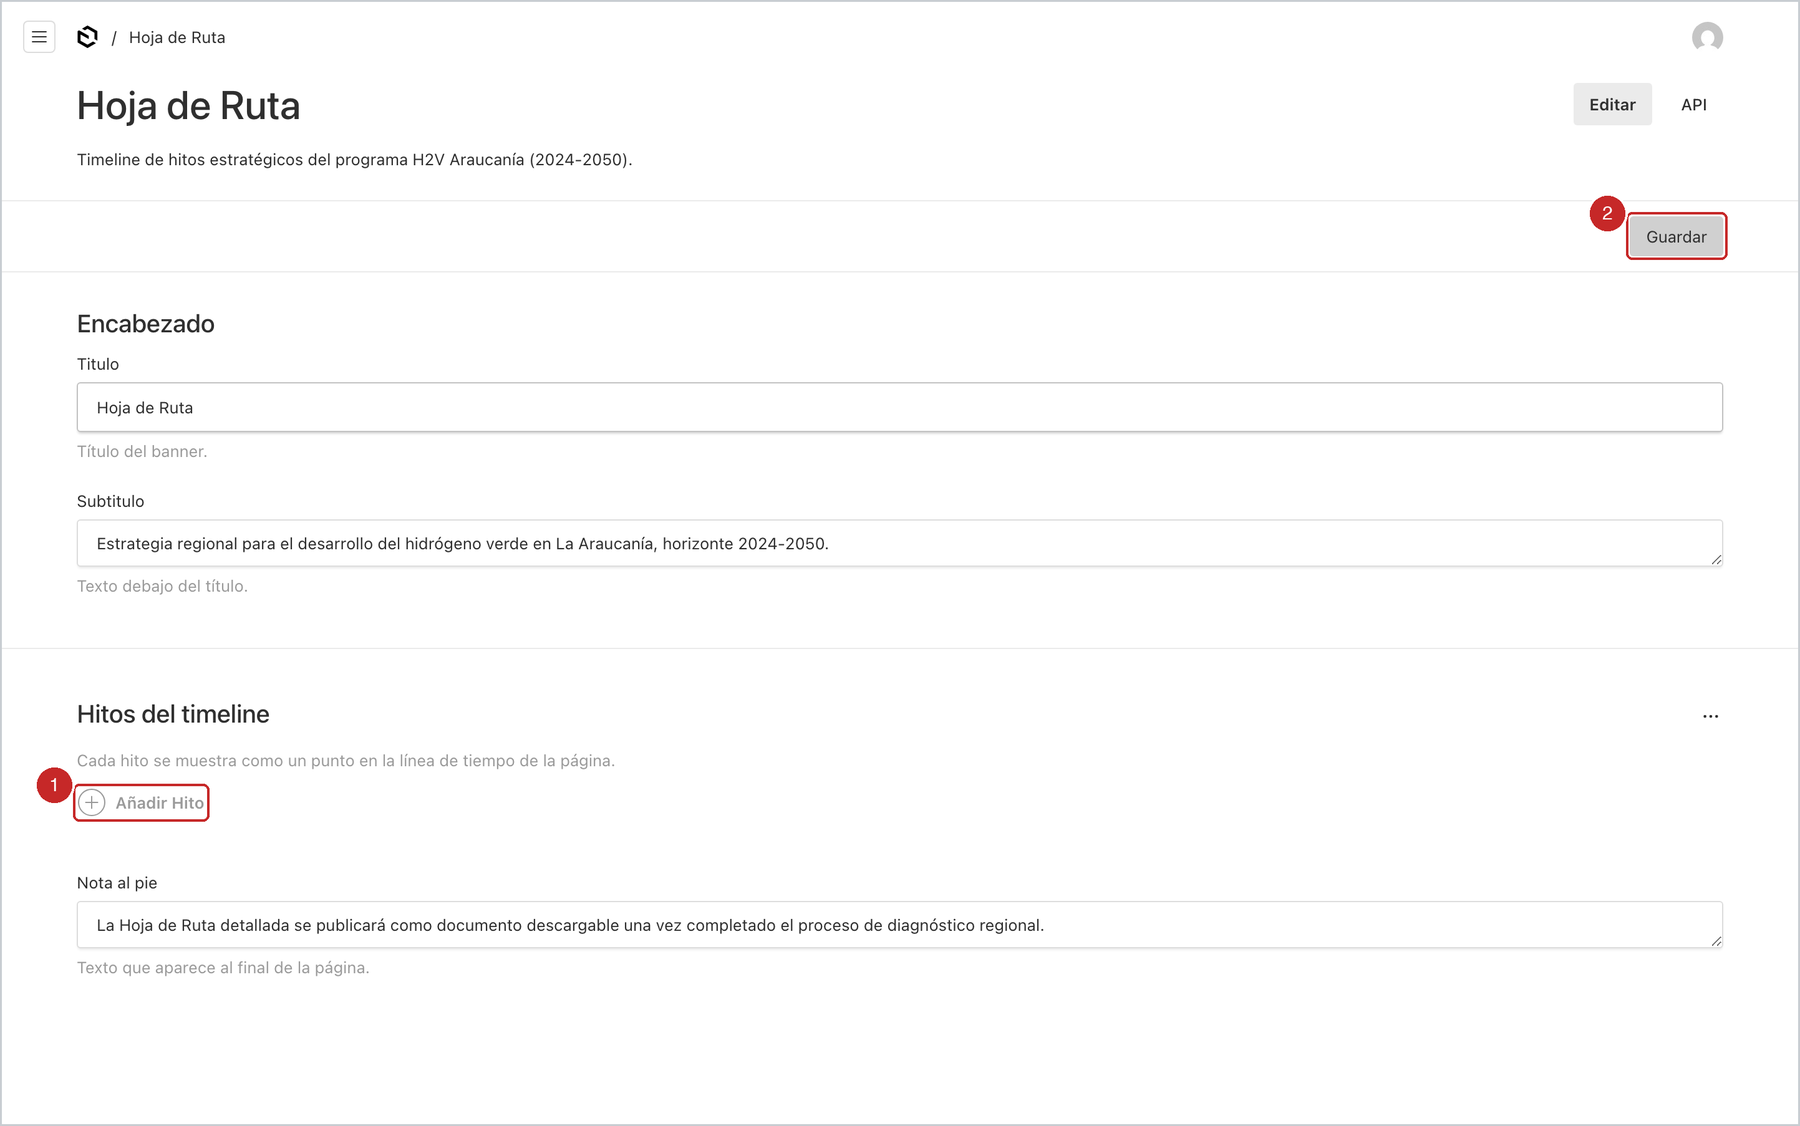
\includegraphics[width=\linewidth,keepaspectratio]{25-hoja-ruta.png}
\caption{Formulario de Hoja de Ruta, con la lista de hitos.}
\end{figure}
\begin{figure}[H]\centering
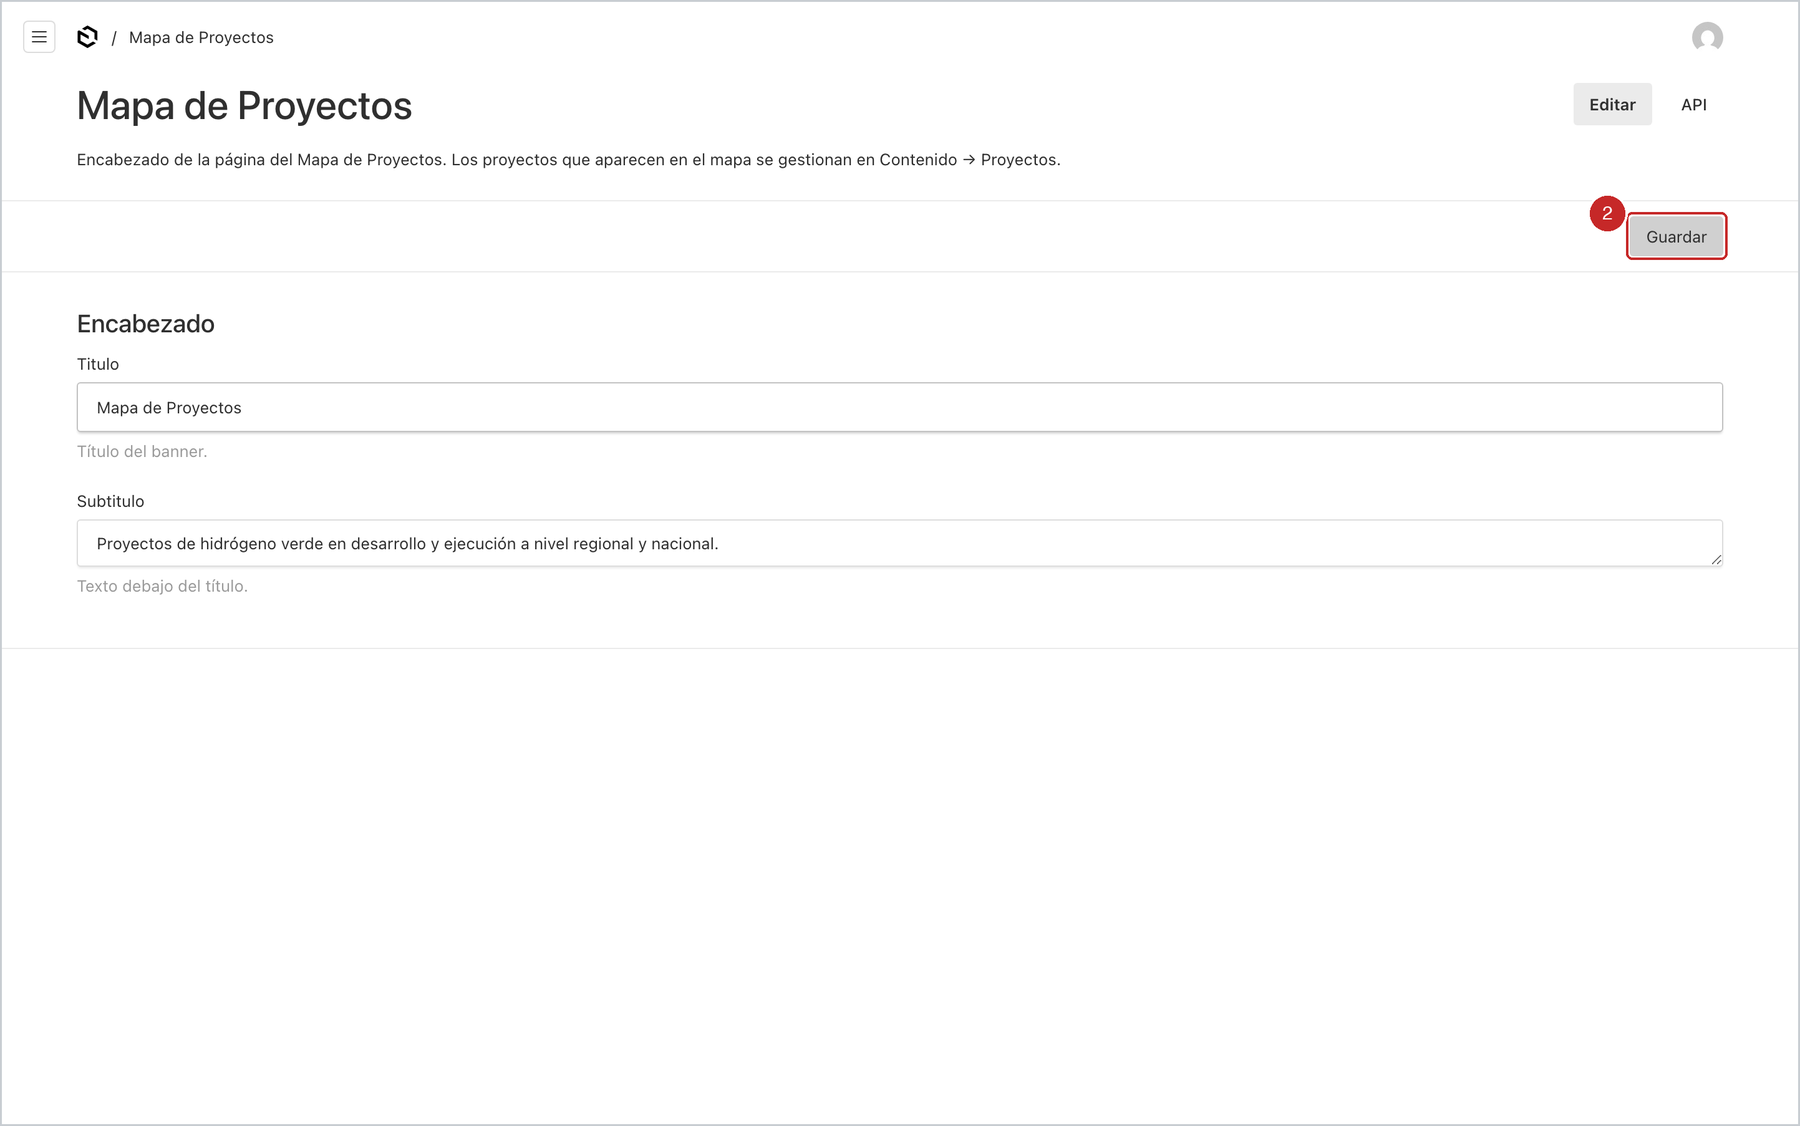
\includegraphics[width=\linewidth,keepaspectratio]{28-mapa-proyectos.png}
\caption{Formulario de Mapa de Proyectos: solo el encabezado de la página del mapa.}
\end{figure}
\section{La Guía de uso dentro del panel}
En \textbf{Ayuda $\rightarrow$ Guía de uso} hay un resumen de este manual, siempre disponible dentro del panel (no se edita; es solo lectura).

\begin{figure}[H]\centering
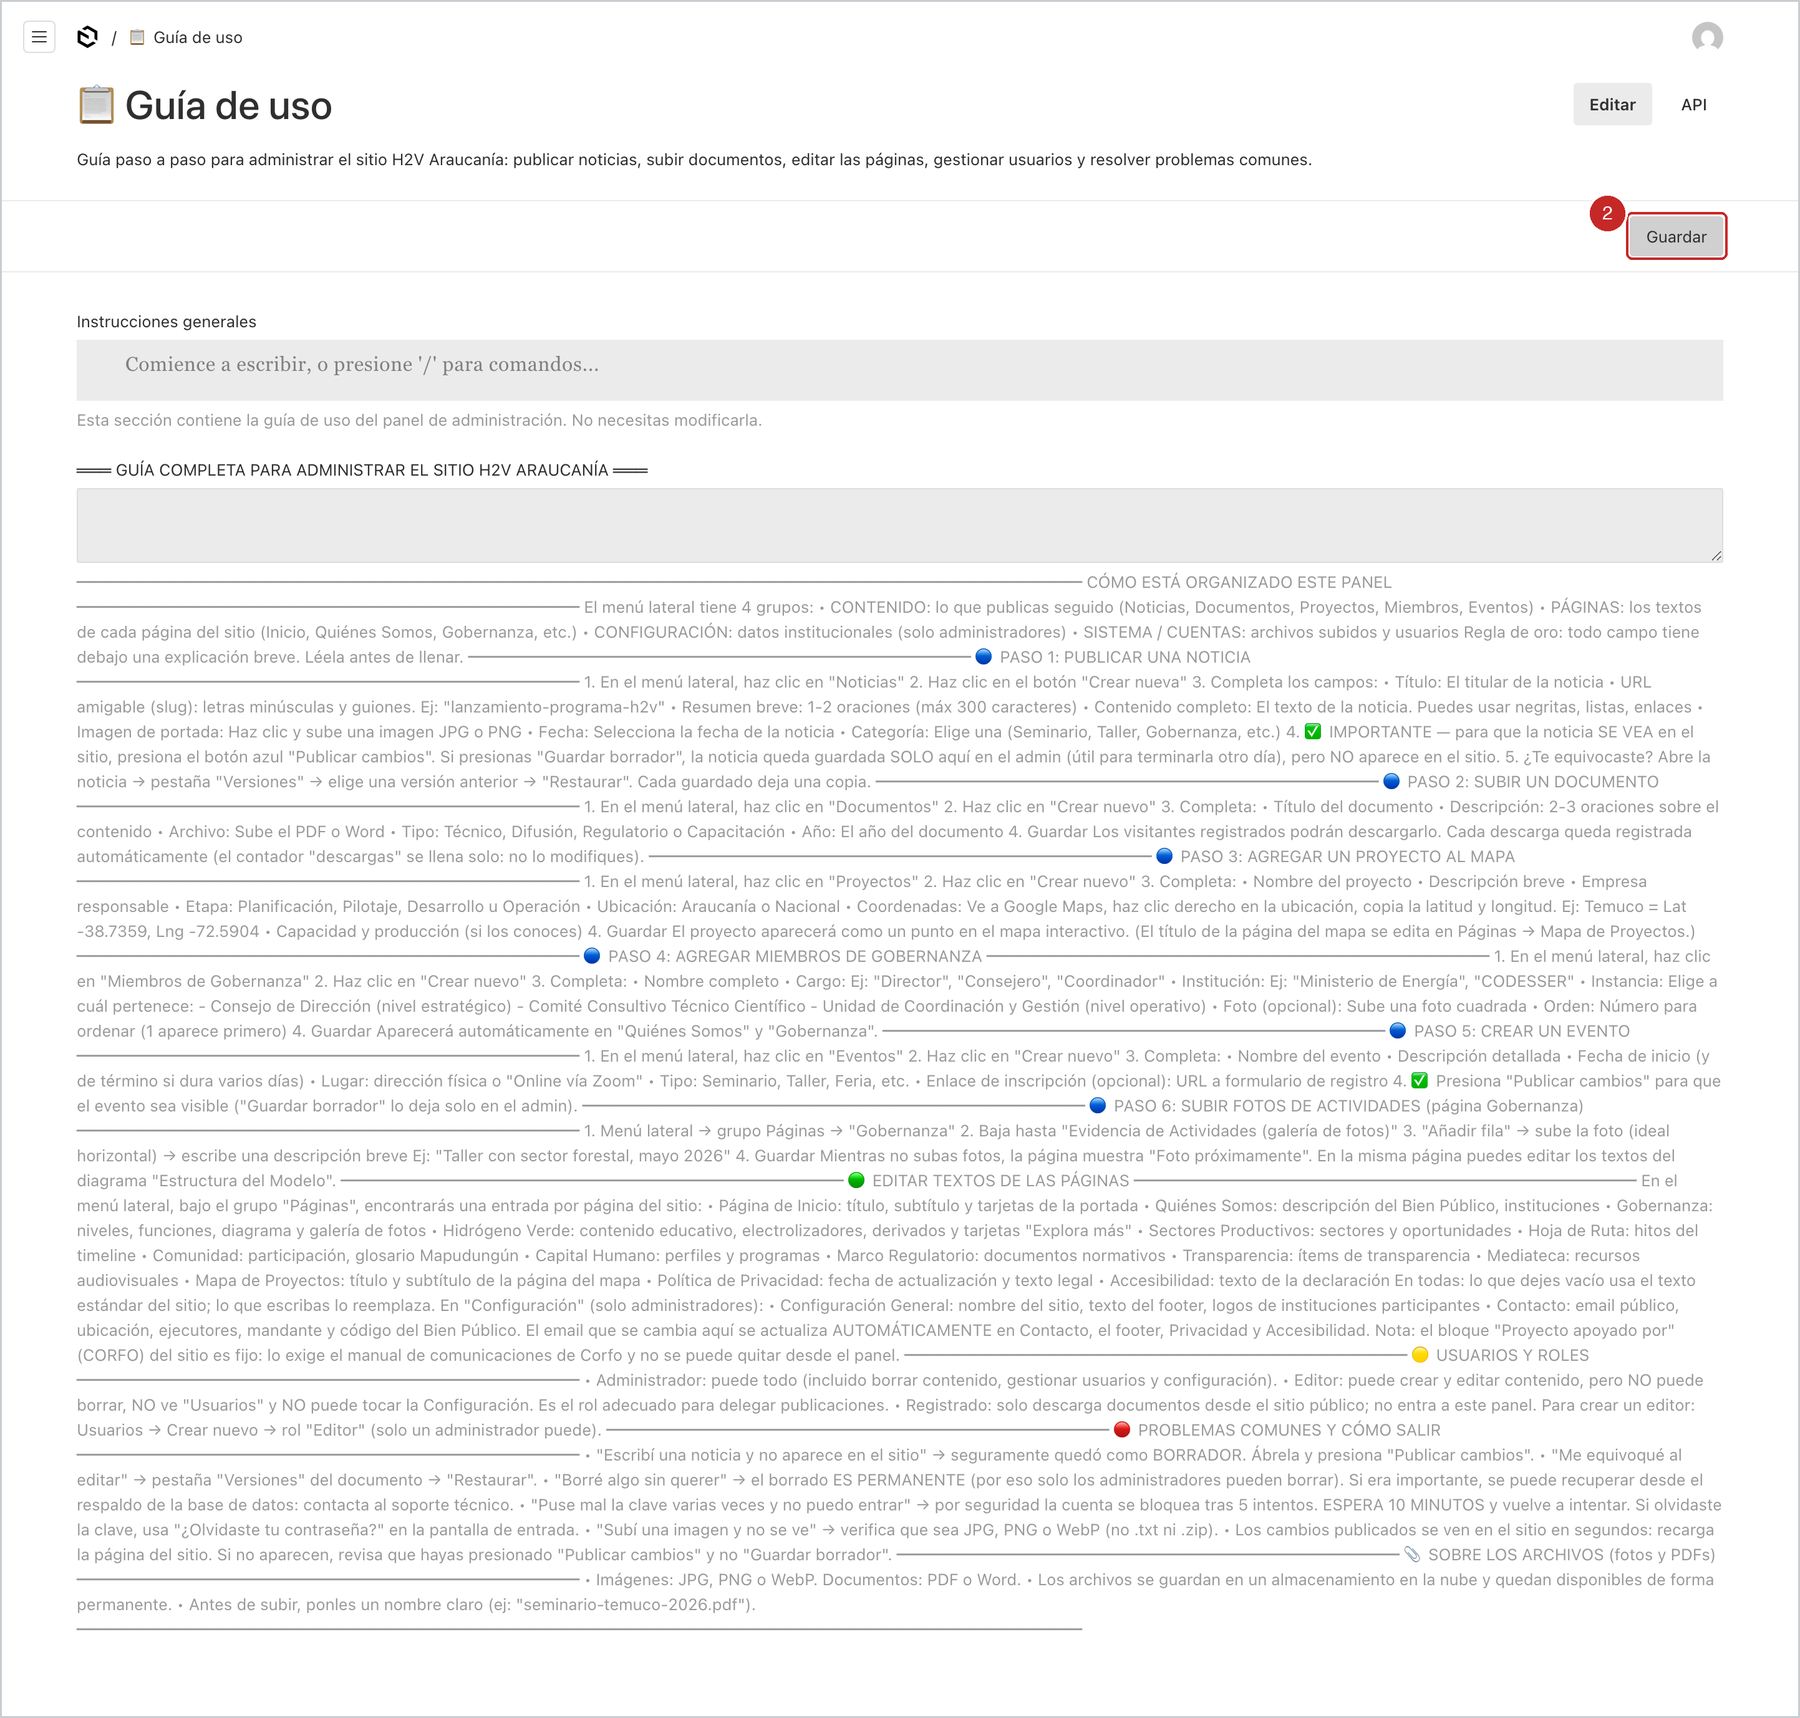
\includegraphics[width=\linewidth,keepaspectratio]{27-guia-admin.png}
\caption{La Guía de uso dentro del panel.}
\end{figure}
\chapter{Usuarios, roles y seguridad}
\section{Los tres roles}
\begin{longtable}{>{\raggedright\arraybackslash}p{0.178\textwidth}>{\raggedright\arraybackslash}p{0.417\textwidth}>{\raggedright\arraybackslash}p{0.335\textwidth}}
\rowcolor{h2vazul}\textbf{\color{white}Rol} & \textbf{\color{white}Qué puede hacer} & \textbf{\color{white}Para quién} \\
\endfirsthead
\rowcolor{h2vazul}\textbf{\color{white}Rol} & \textbf{\color{white}Qué puede hacer} & \textbf{\color{white}Para quién} \\
\endhead
\textbf{Administrador (acceso total)} & Todo: crear y editar contenido, editar las Páginas, la Configuración, crear y eliminar usuarios, eliminar contenido y archivos. & La persona responsable del sitio en la SEREMI (y su respaldo). \\ \midrule
\rowcolor{filaalt}\textbf{Editor (puede publicar contenido)} & Crear y editar noticias, documentos, eventos, proyectos, miembros, capas KMZ y los textos de las Páginas; leer los mensajes de contacto. \textbf{No} puede eliminar, \textbf{no} ve Usuarios y \textbf{no} puede cambiar la Configuración. & Quien publica contenido con frecuencia. \\ \midrule
\textbf{Registrado} & Solo usa el sitio público. \textbf{No entra al panel.} & Hoy no se usa: los documentos se descargan sin cuenta y el sitio no permite que los visitantes se registren solos. \\ \bottomrule
\end{longtable}
\begin{recuadro}{cSeguridad}{bSeguridad}\textbf{\color{bSeguridad}Seguridad:} mantenga \textbf{al menos dos} cuentas de Administrador (titular y respaldo) y no más de las necesarias. Dé rol Editor a quien solo publica contenido.\end{recuadro}
\section{Crear un usuario}
Solo un Administrador puede crear usuarios. Hágalo \textbf{con la persona presente}, frente al mismo computador: ella misma escribirá su contraseña.

\begin{enumerate}
  \item Menú lateral $\rightarrow$ \textbf{Usuarios} (grupo Cuentas y acceso) $\rightarrow$ \textbf{Crear nuevo}.
  \item Complete \textbf{Correo electrónico} (1), \textbf{Nombre completo} (4) y, en la barra lateral, el \textbf{Rol} (5). \textbf{Institución} es opcional.
  \item Pásele el teclado: \textbf{ella misma} escribe su contraseña en \textbf{Nueva Contraseña} (2) y otra vez en \textbf{Confirmar Contraseña} (3). Usted no mira.
  \item Pulse \textbf{Guardar} (6). La persona ya puede entrar con su correo y su contraseña.
\end{enumerate}
\begin{recuadro}{cSeguridad}{bSeguridad}\textbf{\color{bSeguridad}Seguridad:} nunca dicte ni envíe una contraseña por correo o mensajería. Si la persona no puede estar presente, cree la cuenta cuando pueda estarlo. Cuando el sitio tenga dominio propio, también podrá crear su contraseña a distancia con \textbf{¿Olvidaste tu contraseña?} (vea ''Olvidé mi contraseña'').\end{recuadro}
\begin{figure}[H]\centering
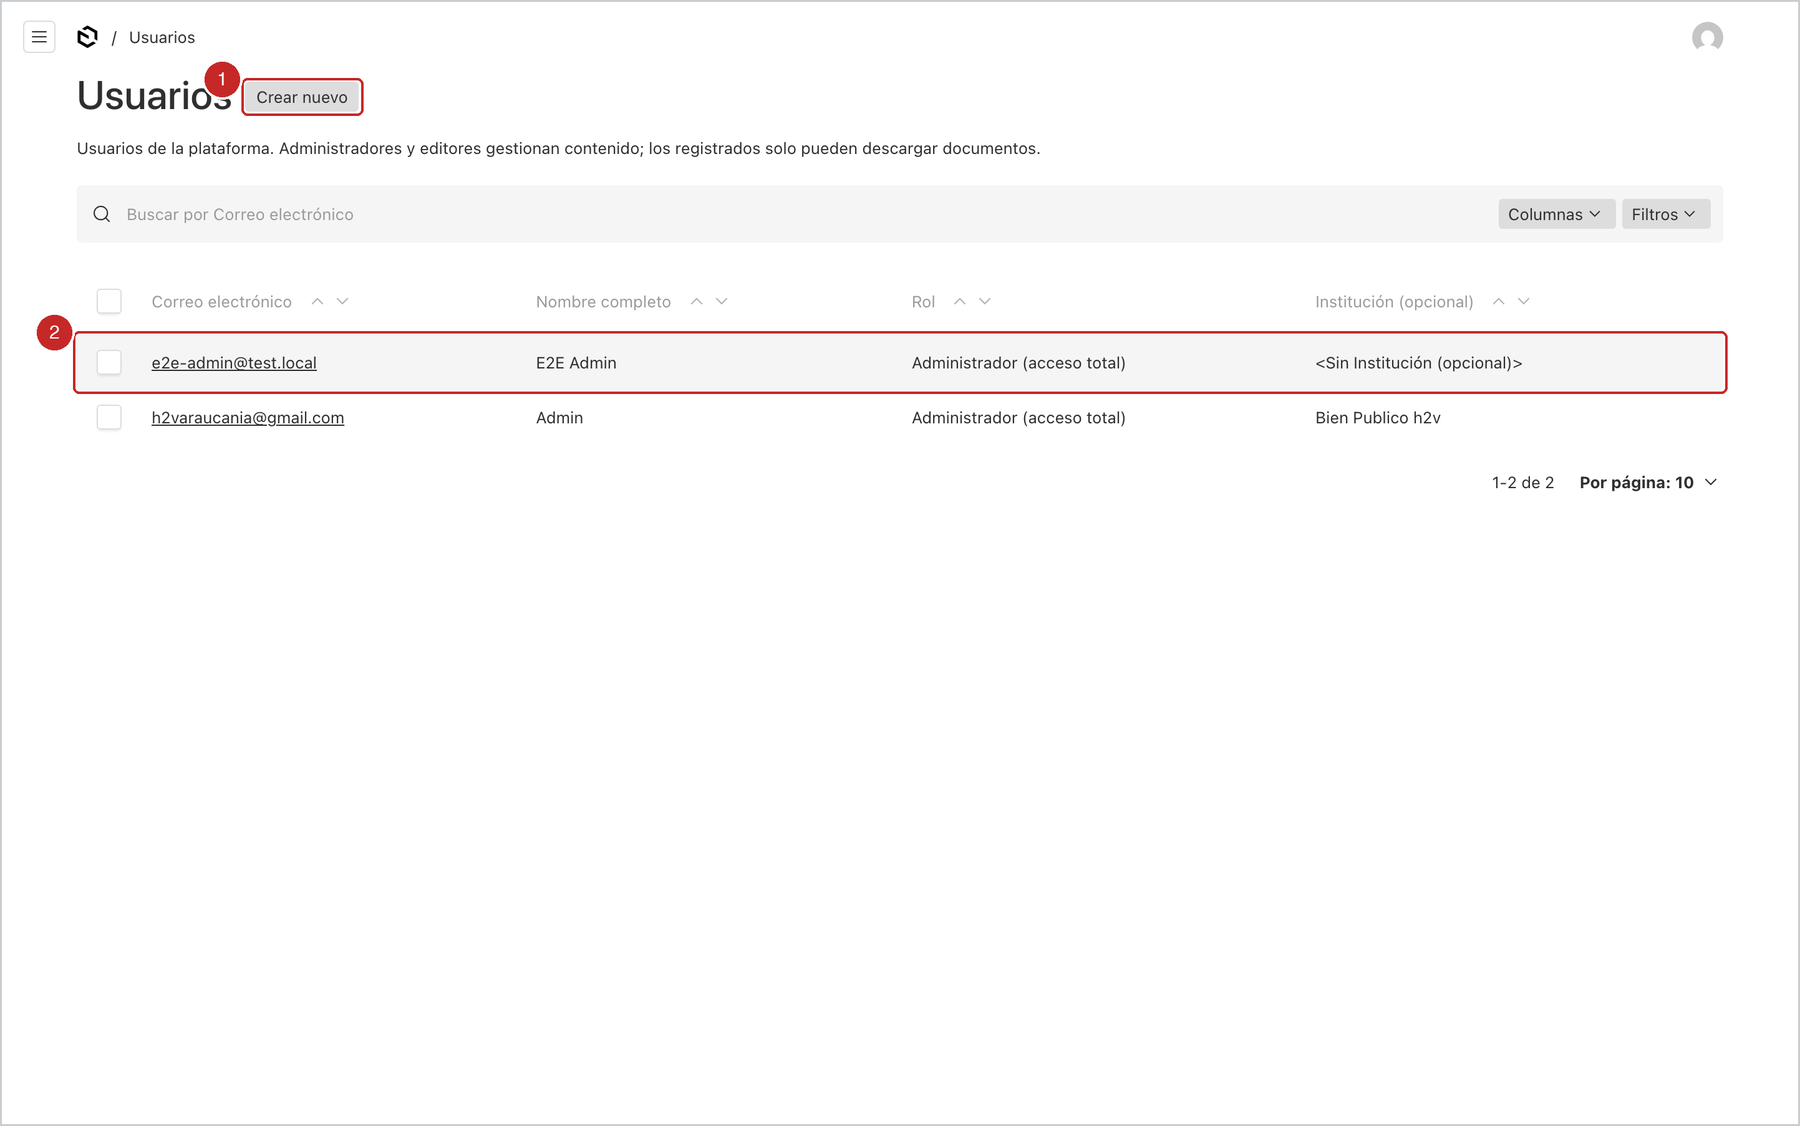
\includegraphics[width=\linewidth,keepaspectratio]{30-usuarios-lista.png}
\caption{Lista de usuarios: Crear nuevo (1) y las cuentas existentes (2).}
\end{figure}
\begin{figure}[H]\centering
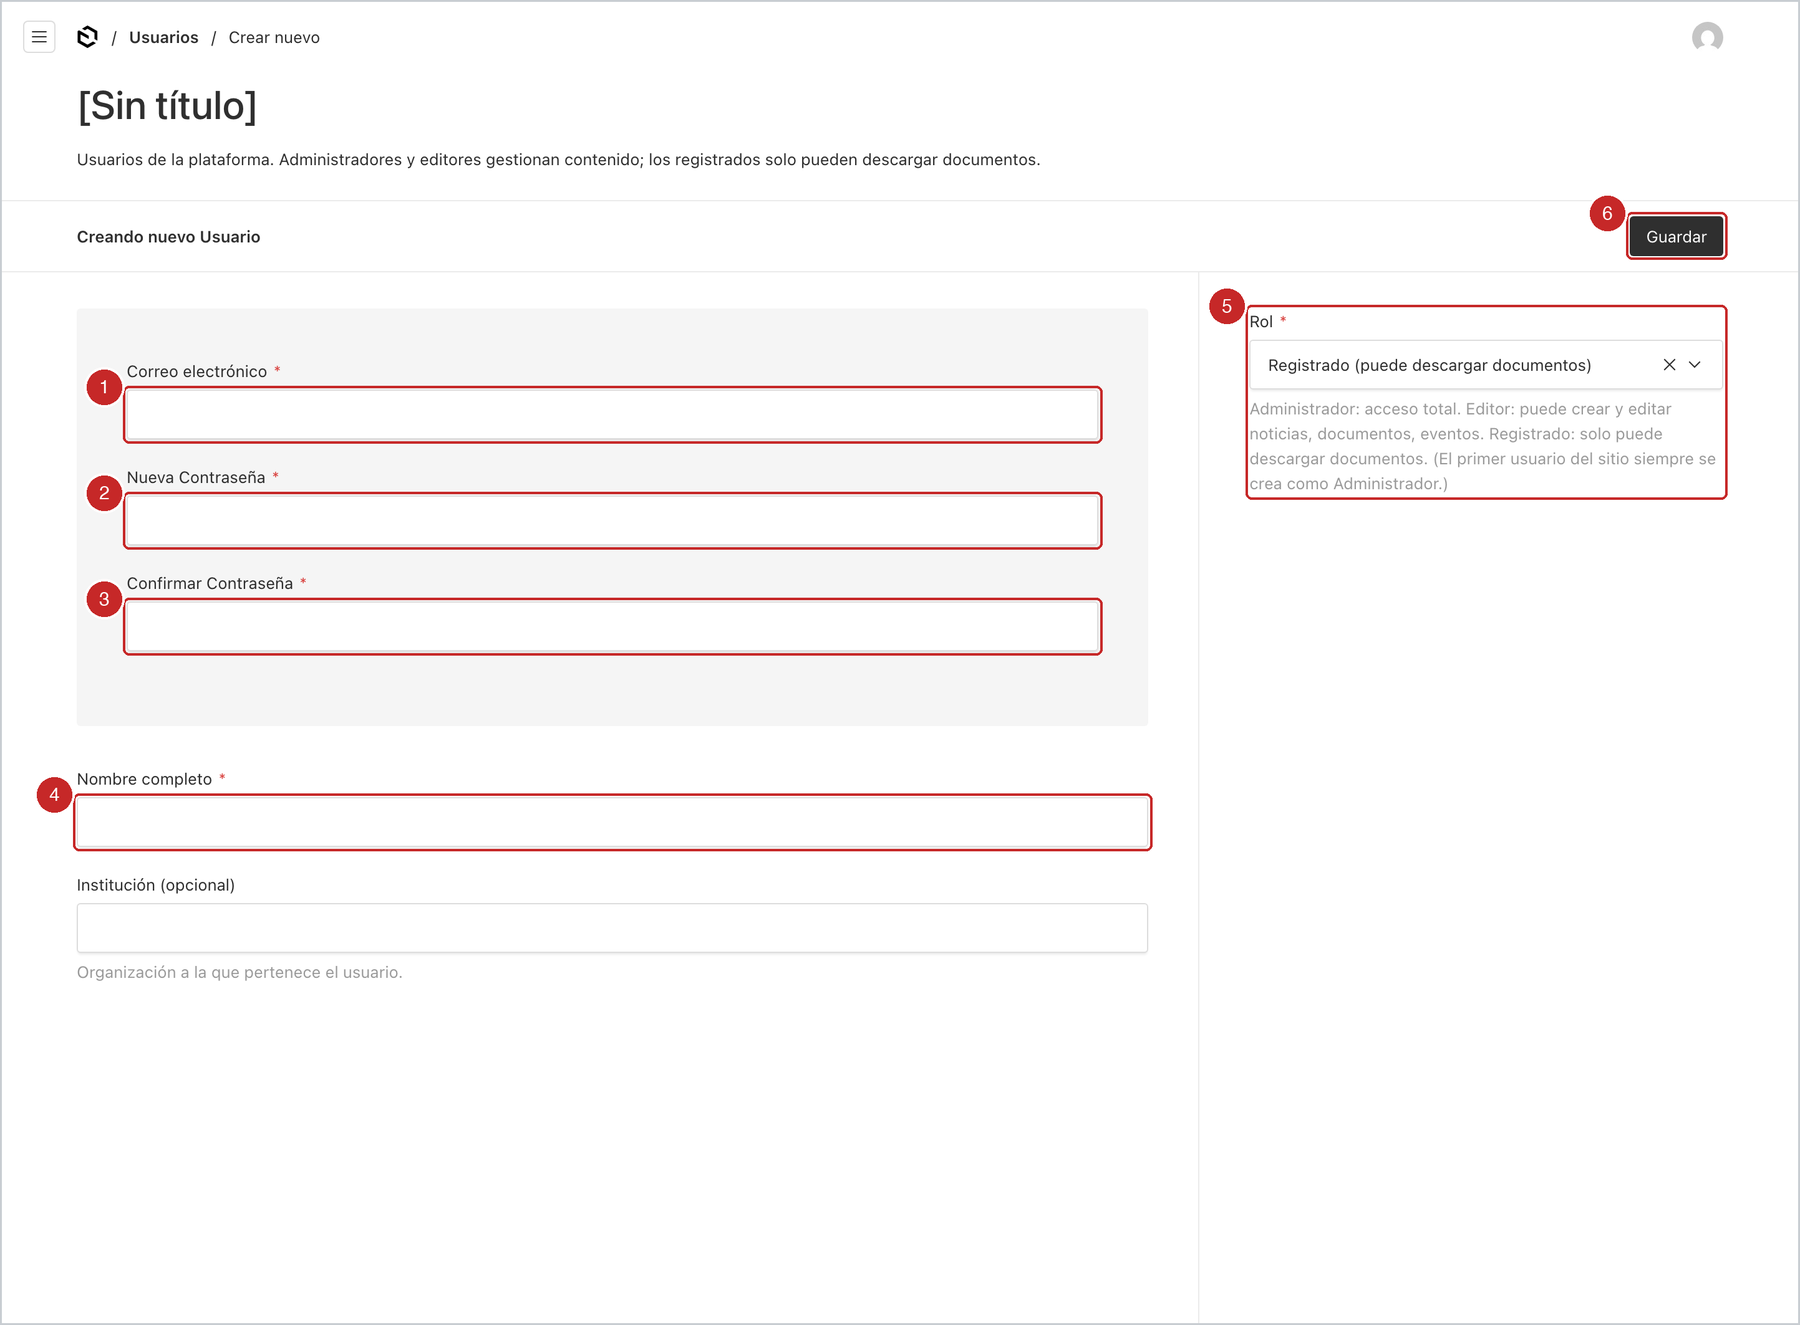
\includegraphics[width=\linewidth,keepaspectratio]{31-usuario-crear.png}
\caption{Formulario de usuario nuevo: correo (1), contraseña (2 y 3), nombre (4), rol (5) y Guardar (6).}
\end{figure}
\textbf{Cambiar el rol, desbloquear o eliminar un usuario}: en la lista de Usuarios haga clic en el correo de la persona; cambie el \textbf{Rol} en la barra lateral y guarde; el botón \textbf{Forzar Desbloqueo} levanta el bloqueo por intentos fallidos; el menú de tres puntos permite \textbf{Eliminar} la cuenta (permanente).

\section{Contraseñas y bloqueo}
\begin{itemize}
  \item Use contraseñas de \textbf{12 caracteres o más}, que mezclen letras, números y símbolos, y que no se usen en otros servicios.
  \item Tras \textbf{5 intentos fallidos} la cuenta se bloquea \textbf{10 minutos} (o hasta que un Administrador la desbloquee).
  \item Si una persona deja la institución, \textbf{elimine o cambie el rol de su cuenta el mismo día}.
\end{itemize}
\chapter{Traspaso del sitio a la SEREMI}
El sitio se entrega a la SEREMI de Energía \textbf{en dos fases}. Así la SEREMI aprende a usar el sitio sin riesgo de dañarlo, y recibe las cuentas de fondo cuando ya tiene práctica y un responsable técnico.

\begin{longtable}{>{\raggedright\arraybackslash}p{0.202\textwidth}>{\raggedright\arraybackslash}p{0.411\textwidth}>{\raggedright\arraybackslash}p{0.221\textwidth}>{\raggedright\arraybackslash}p{0.096\textwidth}}
\rowcolor{h2vazul}\textbf{\color{white}Fase} & \textbf{\color{white}Qué se entrega} & \textbf{\color{white}A quién} & \textbf{\color{white}Cuándo} \\
\endfirsthead
\rowcolor{h2vazul}\textbf{\color{white}Fase} & \textbf{\color{white}Qué se entrega} & \textbf{\color{white}A quién} & \textbf{\color{white}Cuándo} \\
\endhead
\textbf{Fase 1: el contenido} & Usuarios propios del panel para publicar noticias, eventos, documentos y proyectos. & Dos personas designadas por la SEREMI (titular y respaldo). & Ahora. \\ \midrule
\rowcolor{filaalt}\textbf{Fase 2: la infraestructura} & Las cuentas de fondo: el correo central, el alojamiento (Vercel), la base de datos (Neon), el código (GitHub) y el envío de correos (Resend). & Un responsable técnico designado por la SEREMI. & Meta: enero de 2027. \\ \bottomrule
\end{longtable}
\begin{recuadro}{cSeguridad}{bSeguridad}\textbf{\color{bSeguridad}Seguridad:} regla de oro para las dos fases. Ninguna contraseña se dicta, se anota en un papel compartido ni se envía por correo o por mensajería. \textbf{Cada persona crea la suya}, en el momento, desde su propio computador o teléfono.\end{recuadro}
El detalle completo, con casillas para marcar cada paso y las hojas para firmar (la constancia de la Fase 1 y el acta final de la Fase 2), está en el documento \textbf{Protocolo de entrega del sitio web H2V Araucanía}, que se entrega junto con este manual.

\section{Fase 1: entrega del contenido}
\textbf{Antes de la reunión} (lo prepara el responsable del programa):

\begin{enumerate}
  \item Pedir a la SEREMI el nombre, cargo y correo institucional de \textbf{dos personas}: una titular y una de respaldo.
  \item Revisar que el contenido publicado esté listo para ser visto por el público.
  \item Guardar los \textbf{códigos de respaldo} de la cuenta central de Google (\texttt{h2varaucania@gmail.com}): \textbf{Seguridad} $\rightarrow$ \textbf{Verificación en dos pasos} $\rightarrow$ \textbf{Códigos de respaldo}. Imprimirlos y guardarlos en un sobre cerrado. Cada código permite entrar una vez sin teléfono ni huella.
\end{enumerate}
\textbf{En la reunión} (unos 45 minutos):

\begin{enumerate}
  \item El Administrador crea un usuario para cada persona, con rol \textbf{Editor} (vea ''Crear un usuario''). Al llegar a la contraseña le pasa el teclado: \textbf{cada persona escribe la suya}, sin que nadie la vea.
  \item Cada persona entra al panel con su correo y su contraseña, y comprueba que ve el Panel de Control.
  \item Práctica guiada con este manual: cada persona crea una noticia de prueba, la publica y la ve en el sitio. Después un Administrador la elimina (un Editor no puede eliminar contenido, y eso es a propósito). También revisan juntos \textbf{Mensajes de contacto}.
  \item Se entrega este manual (PDF y Word) y el protocolo de entrega.
  \item El Administrador del programa cambia su propia contraseña por una nueva y robusta.
  \item Se firma la \textbf{constancia de la Fase 1} (está en el protocolo).
\end{enumerate}
\begin{recuadro}{cResultado}{bResultado}\textbf{\color{bResultado}Resultado:} la SEREMI publica el contenido del sitio con sus propios usuarios. El programa sigue a cargo del funcionamiento del sitio y de sus respaldos.\end{recuadro}
\section{Fase 2: traspaso de la infraestructura}
\textbf{Condiciones previas:} la SEREMI usa el panel sin ayuda y designó un responsable técnico (propio o un servicio de mantención). El respaldo diario de la base de datos ya funciona.

\textbf{En la reunión} (unos 60 minutos, idealmente presencial, con el responsable técnico):

\begin{enumerate}
  \item \textbf{Cuenta central de Google} (\texttt{h2varaucania@gmail.com}), que es la llave maestra: la persona de la SEREMI pone una contraseña nueva elegida por ella, registra su propio teléfono en la verificación en dos pasos, cambia el teléfono y el correo de recuperación por los suyos y genera sus propios códigos de respaldo. Después el programa elimina su teléfono y sus llaves de acceso, y se cierra la sesión en todos los dispositivos.
  \item \textbf{Alojamiento (Vercel) y base de datos (Neon):} se entra a ellos con la cuenta central, así que pasan junto con ella. Se comprueba que el responsable técnico puede entrar.
  \item \textbf{Código (GitHub):} la cuenta \texttt{h2varaucania} se entrega del mismo modo que la cuenta central. Se retira la cuenta de colaborador de la Universidad, salvo que se acuerde mantener soporte.
  \item \textbf{Envío de correos (Resend):} se confirma con qué cuenta se creó y se entrega del mismo modo.
  \item \textbf{Llave secreta del sitio:} el responsable técnico cambia en Vercel el valor de la variable \texttt{PAYLOAD\_\allowbreak{}SECRET} por un texto largo al azar y vuelve a publicar el sitio. Efecto: todas las personas deben iniciar sesión de nuevo.
  \item \textbf{Alojamiento definitivo:} el plan gratuito de Vercel está destinado a uso personal y no comercial. Para un sitio institucional corresponde un plan pagado o un servidor propio de la SEREMI.
  \item \textbf{Usuarios del panel:} el responsable técnico pasa a ser \textbf{Administrador}; las cuentas del programa se eliminan o pasan a Editor.
  \item Se firma el \textbf{acta final} (está en el protocolo). Desde esa fecha, la operación del sitio queda a cargo de la SEREMI.
\end{enumerate}
\chapter{Problemas frecuentes}
\begin{longtable}{>{\raggedright\arraybackslash}p{0.260\textwidth}>{\raggedright\arraybackslash}p{0.229\textwidth}>{\raggedright\arraybackslash}p{0.441\textwidth}}
\rowcolor{h2vazul}\textbf{\color{white}Problema} & \textbf{\color{white}Causa probable} & \textbf{\color{white}Solución} \\
\endfirsthead
\rowcolor{h2vazul}\textbf{\color{white}Problema} & \textbf{\color{white}Causa probable} & \textbf{\color{white}Solución} \\
\endhead
Publiqué una noticia y no aparece en el sitio & Quedó en \textbf{Borrador} & Ábrala y pulse \textbf{Publicar cambios}. Luego recargue la página del sitio. \\ \midrule
\rowcolor{filaalt}Cambié un texto de una Página y no lo veo & No pulsó Guardar, o el navegador muestra una copia antigua & Compruebe que pulsó \textbf{Guardar}; recargue el sitio con Ctrl + F5 (Cmd + Shift + R en Mac). \\ \midrule
Al guardar sale un mensaje rojo ''El siguiente campo es inválido'' & Falta un campo obligatorio o supera el largo máximo & Busque el campo marcado en rojo (el mensaje lo nombra), corríjalo y vuelva a guardar. \\ \midrule
\rowcolor{filaalt}''Valor duplicado'' en la URL amigable & Ya existe otra noticia con esa URL & Cambie el texto de la URL amigable (por ejemplo, agregue el año). \\ \midrule
Subí una imagen y no se ve & Formato no aceptado o archivo dañado & Use JPG, PNG o WebP; vuelva a exportar la imagen y súbala de nuevo. \\ \midrule
\rowcolor{filaalt}El archivo no se sube o tarda mucho & Es muy pesado & Reduzca el tamaño (imágenes: menos de 5 MB; PDF: comprímalo). \\ \midrule
El punto del proyecto aparece en el mar o en otro país & Latitud y longitud invertidas o sin signo negativo & Revise las coordenadas: en Chile ambas son negativas; la latitud va primero. \\ \midrule
\rowcolor{filaalt}No puedo entrar: ''demasiados intentos'' & Bloqueo por 5 intentos fallidos & Espere 10 minutos o pida a un Administrador que use \textbf{Forzar Desbloqueo}. \\ \midrule
No me llega el correo de ''¿Olvidaste tu contraseña?'' & Mientras el sitio no tenga dominio propio, ese correo no llega a los correos institucionales & Pida a un Administrador que le deje escribir una contraseña nueva (vea ''Olvidé mi contraseña''). \\ \midrule
\rowcolor{filaalt}No veo Usuarios ni Configuración en el menú & Su rol es Editor & Es lo esperado. Pida a un Administrador el cambio. \\ \midrule
Me equivoqué al editar una noticia o evento & — & Pestaña \textbf{Versiones} $\rightarrow$ elija la versión anterior $\rightarrow$ \textbf{Restaurar}. \\ \midrule
\rowcolor{filaalt}Borré algo por error & Eliminar es permanente & No se puede deshacer desde el panel. Contacte al soporte técnico: puede recuperarse desde el respaldo de la base de datos. \\ \midrule
La página del panel se ve en blanco o con un error & Falla temporal o cambio técnico & Recargue la página. Si persiste, anote la dirección y la hora y avise al soporte técnico. \\ \midrule
\rowcolor{filaalt}No me llegan por correo los mensajes del formulario de contacto & El aviso por correo depende de un servicio que aún no tiene dominio propio & Los mensajes no se pierden: léalos en Contenido $\rightarrow$ \textbf{Mensajes de contacto}. Para recibir también el aviso por correo, el soporte técnico debe configurar el dominio (Anexo D). \\ \bottomrule
\end{longtable}
\chapter{Anexos}
\section{Anexo A. Quiero cambiar... ¿a dónde voy?}
\begin{longtable}{>{\raggedright\arraybackslash}p{0.331\textwidth}>{\raggedright\arraybackslash}p{0.599\textwidth}}
\rowcolor{h2vazul}\textbf{\color{white}Quiero...} & \textbf{\color{white}Voy a...} \\
\endfirsthead
\rowcolor{h2vazul}\textbf{\color{white}Quiero...} & \textbf{\color{white}Voy a...} \\
\endhead
Publicar una noticia & Contenido $\rightarrow$ Noticias $\rightarrow$ Crear nuevo $\rightarrow$ Publicar cambios \\ \midrule
\rowcolor{filaalt}Corregir una noticia publicada & Contenido $\rightarrow$ Noticias $\rightarrow$ (la noticia) $\rightarrow$ editar $\rightarrow$ Publicar cambios \\ \midrule
Que una noticia deje de verse & Contenido $\rightarrow$ Noticias $\rightarrow$ (la noticia) $\rightarrow$ menú de tres puntos $\rightarrow$ despublicar \\ \midrule
\rowcolor{filaalt}Crear un evento & Contenido $\rightarrow$ Eventos $\rightarrow$ Crear nuevo $\rightarrow$ Publicar cambios \\ \midrule
Subir un documento para descarga & Contenido $\rightarrow$ Documentos $\rightarrow$ Crear nuevo $\rightarrow$ Guardar \\ \midrule
\rowcolor{filaalt}Agregar un proyecto al mapa & Contenido $\rightarrow$ Proyectos $\rightarrow$ Crear nuevo $\rightarrow$ Guardar \\ \midrule
Dibujar la forma (polígono) de un proyecto en el mapa & Google Earth $\rightarrow$ Archivo $\rightarrow$ Exportar como archivo KML; luego Contenido $\rightarrow$ Capas geográficas (KMZ) $\rightarrow$ Crear nuevo; luego Contenido $\rightarrow$ Proyectos $\rightarrow$ (el proyecto) $\rightarrow$ Capa geográfica \\ \midrule
\rowcolor{filaalt}Quitar la forma de un proyecto del mapa & Contenido $\rightarrow$ Proyectos $\rightarrow$ (el proyecto) $\rightarrow$ Capa geográfica $\rightarrow$ X $\rightarrow$ Guardar \\ \midrule
Encender o apagar las funciones KMZ del mapa & No se hace desde el panel: lo activa el equipo informático (Anexo D) \\ \midrule
\rowcolor{filaalt}Cambiar una persona del Comité Estratégico & Contenido $\rightarrow$ Miembros de Gobernanza $\rightarrow$ (la fila del cargo) $\rightarrow$ cambiar nombre $\rightarrow$ Guardar \\ \midrule
Poner nombre a un cargo ''Por definir'' de la Unidad de Coordinación & Contenido $\rightarrow$ Miembros de Gobernanza $\rightarrow$ (la fila) $\rightarrow$ cambiar nombre e institución $\rightarrow$ Guardar \\ \midrule
\rowcolor{filaalt}Subir fotos de una sesión o taller & Páginas $\rightarrow$ Gobernanza $\rightarrow$ Evidencia de Actividades $\rightarrow$ Añadir fila \\ \midrule
Cambiar el título o subtítulo de la portada & Páginas $\rightarrow$ Página de Inicio $\rightarrow$ Sección Hero \\ \midrule
\rowcolor{filaalt}Cambiar una cifra de la portada (KPI) & Páginas $\rightarrow$ Página de Inicio $\rightarrow$ Banda de indicadores \\ \midrule
Cambiar el texto ''El Bien Público'' & Páginas $\rightarrow$ Quiénes Somos $\rightarrow$ El Bien Público \\ \midrule
\rowcolor{filaalt}Agregar una institución participante (con logo) & Configuración $\rightarrow$ Configuración General $\rightarrow$ Logos institucionales (portada y pie de página) y Páginas $\rightarrow$ Quiénes Somos $\rightarrow$ Instituciones participantes (página Quiénes Somos) \\ \midrule
Cambiar el correo o la ubicación de contacto & Configuración $\rightarrow$ Contacto $\rightarrow$ Datos institucionales \\ \midrule
\rowcolor{filaalt}Cambiar las opciones de asunto del formulario & Configuración $\rightarrow$ Contacto $\rightarrow$ Formulario $\rightarrow$ Opciones de asunto \\ \midrule
Leer lo que escriben los visitantes en el formulario de Contacto & Contenido $\rightarrow$ Mensajes de contacto $\rightarrow$ (el mensaje) $\rightarrow$ responder desde su correo $\rightarrow$ marcar Atendido $\rightarrow$ Guardar \\ \midrule
\rowcolor{filaalt}Cambiar textos del pie de página & Configuración $\rightarrow$ Configuración General \\ \midrule
Cambiar el nombre del sitio (pestaña del navegador) & Configuración $\rightarrow$ Configuración General $\rightarrow$ Nombre del sitio \\ \midrule
\rowcolor{filaalt}Editar la Hoja de Ruta & Páginas $\rightarrow$ Hoja de Ruta $\rightarrow$ Hitos del timeline \\ \midrule
Editar el contenido educativo de H2V & Páginas $\rightarrow$ Hidrógeno Verde \\ \midrule
\rowcolor{filaalt}Crear una cuenta para un colega & Cuentas y acceso $\rightarrow$ Usuarios $\rightarrow$ Crear nuevo (con la persona presente: ella escribe su contraseña) \\ \midrule
Ponerle una contraseña nueva a quien la olvidó & Cuentas y acceso $\rightarrow$ Usuarios $\rightarrow$ (su correo) $\rightarrow$ Cambiar contraseña (con la persona presente: ella la escribe) $\rightarrow$ Guardar \\ \midrule
\rowcolor{filaalt}Cambiar mi contraseña & Mi cuenta (círculo superior derecho) $\rightarrow$ Cambiar contraseña \\ \midrule
Ver cuántas veces se descargó un documento & Contenido $\rightarrow$ Documentos $\rightarrow$ (el documento) $\rightarrow$ campo Descargas; o Sistema $\rightarrow$ Registro de Descargas \\ \midrule
\rowcolor{filaalt}Leer la guía rápida dentro del panel & Ayuda $\rightarrow$ Guía de uso \\ \midrule
Entregar el sitio a la SEREMI & Capítulo ''Traspaso del sitio a la SEREMI'' y el protocolo de entrega \\ \bottomrule
\end{longtable}
\section{Anexo B. Formatos y tamaños recomendados}
\begin{longtable}{>{\raggedright\arraybackslash}p{0.309\textwidth}>{\raggedright\arraybackslash}p{0.206\textwidth}>{\raggedright\arraybackslash}p{0.415\textwidth}}
\rowcolor{h2vazul}\textbf{\color{white}Elemento} & \textbf{\color{white}Formato} & \textbf{\color{white}Tamaño recomendado} \\
\endfirsthead
\rowcolor{h2vazul}\textbf{\color{white}Elemento} & \textbf{\color{white}Formato} & \textbf{\color{white}Tamaño recomendado} \\
\endhead
Imagen de portada de noticia & JPG o PNG & 1200 x 630 píxeles, menos de 1 MB \\ \midrule
\rowcolor{filaalt}Imagen de evento (afiche) & JPG o PNG & Vertical u horizontal, menos de 2 MB \\ \midrule
Foto de persona (gobernanza) & JPG o PNG & Cuadrada, mínimo 200 x 200 \\ \midrule
\rowcolor{filaalt}Foto de galería (Gobernanza) & JPG & Horizontal, 1600 píxeles de ancho aprox. \\ \midrule
Logo de institución & PNG con fondo transparente (o SVG) & Al menos 400 píxeles de ancho \\ \midrule
\rowcolor{filaalt}Portada de documento & JPG o PNG & 800 x 600 aprox. \\ \midrule
Documento para descarga & PDF (también Word, PowerPoint, Excel) & Lo más liviano posible; comprima los PDF grandes \\ \midrule
\rowcolor{filaalt}Capa geográfica de un proyecto & KMZ o KML (guardado desde Google Earth) & Menos de 4 MB; el predio de un proyecto pesa unos pocos KB \\ \midrule
Imagen dentro del texto de una noticia & JPG o PNG & 1200 píxeles de ancho máximo \\ \bottomrule
\end{longtable}
Límites de texto más importantes: título de noticia 120 caracteres; resumen 300; descripción de documento 400; descripción de proyecto 400; URL amigable solo minúsculas, números y guiones.

\section{Anexo C. Glosario}
\begin{longtable}{>{\raggedright\arraybackslash}p{0.198\textwidth}>{\raggedright\arraybackslash}p{0.732\textwidth}}
\rowcolor{h2vazul}\textbf{\color{white}Término} & \textbf{\color{white}Significado} \\
\endfirsthead
\rowcolor{h2vazul}\textbf{\color{white}Término} & \textbf{\color{white}Significado} \\
\endhead
\textbf{Panel} (o admin) & El área privada del sitio, en \url{/admin}, desde donde se edita todo. \\ \midrule
\rowcolor{filaalt}\textbf{Sitio público} & Lo que ve cualquier visitante. \\ \midrule
\textbf{Colección} & Una lista de elementos del mismo tipo (noticias, documentos, usuarios...). \\ \midrule
\rowcolor{filaalt}\textbf{Global} (Página) & Un formulario único con los textos de una página del sitio. \\ \midrule
\textbf{Borrador} & Contenido guardado en el panel que no se ve en el sitio. \\ \midrule
\rowcolor{filaalt}\textbf{Publicar} & Hacer visible en el sitio un borrador. \\ \midrule
\textbf{Versión} & Copia guardada de un contenido cada vez que se publica; permite volver atrás. \\ \midrule
\rowcolor{filaalt}\textbf{URL amigable} (slug) & El identificador en la dirección web de una noticia (\url{/noticias/mi-noticia}). \\ \midrule
\textbf{Campo} & Cada casilla de un formulario. \\ \midrule
\rowcolor{filaalt}\textbf{Barra lateral} & La columna derecha de un formulario, con los datos de clasificación. \\ \midrule
\textbf{Archivo multimedia} (Media) & Cualquier imagen o documento subido al sitio. \\ \midrule
\rowcolor{filaalt}\textbf{Descripción del archivo} (alt) & Texto corto que describe un archivo subido; obligatorio. \\ \midrule
\textbf{Rol} & Nivel de permisos de una cuenta: Administrador, Editor o Registrado. \\ \midrule
\rowcolor{filaalt}\textbf{KPI} & Cifra destacada de la portada (indicador). \\ \midrule
\textbf{Kicker / eyebrow} & Palabra o línea pequeña que va encima de un título. \\ \midrule
\rowcolor{filaalt}\textbf{KMZ / KML} & Archivo en que Google Earth guarda un dibujo sobre el mapa (puntos, líneas o formas). El KMZ es la versión comprimida del KML. \\ \midrule
\textbf{Capa geográfica} & Un archivo KMZ o KML subido al panel. Se une a un proyecto para dibujar su forma en el mapa. \\ \bottomrule
\end{longtable}
\section{Anexo D. Ficha técnica de la plataforma (para el equipo informático)}
Esta ficha resume la información que el equipo informático de la SEREMI necesita conocer. El detalle completo está en el repositorio del proyecto, en el documento \texttt{docs/INTERFAZ\_\allowbreak{}ADMIN\_\allowbreak{}TECNICA.md}, y en el estándar \texttt{docs/EDITABILIDAD\_\allowbreak{}TOTAL.md}.

\begin{longtable}{>{\raggedright\arraybackslash}p{0.202\textwidth}>{\raggedright\arraybackslash}p{0.371\textwidth}>{\raggedright\arraybackslash}p{0.357\textwidth}}
\rowcolor{h2vazul}\textbf{\color{white}Componente} & \textbf{\color{white}Qué es} & \textbf{\color{white}Dónde está} \\
\endfirsthead
\rowcolor{h2vazul}\textbf{\color{white}Componente} & \textbf{\color{white}Qué es} & \textbf{\color{white}Dónde está} \\
\endhead
Sitio web y panel & Aplicación Next.js 16 con el gestor de contenidos Payload CMS 3 (panel en \url{/admin}). Idioma del panel: español. & Código en el repositorio Git del proyecto (carpeta \texttt{h2v-araucania}). \\ \midrule
\rowcolor{filaalt}Alojamiento (hosting) & Vercel. Cada cambio en la rama principal del repositorio se despliega solo. & Proyecto \texttt{h2v-araucania} en Vercel; dirección actual \url{https://h2v-araucania.vercel.app} (a reemplazar por el dominio institucional cuando se contrate). \\ \midrule
Base de datos & PostgreSQL administrado (Neon). Contiene todo el contenido editable. & Conexión configurada en Vercel (variable \texttt{DATABASE\_\allowbreak{}URI}). \\ \midrule
\rowcolor{filaalt}Archivos subidos & Vercel Blob (almacenamiento de imágenes y PDF subidos desde el panel). & Conectado al proyecto en Vercel (\texttt{BLOB\_\allowbreak{}READ\_\allowbreak{}WRITE\_\allowbreak{}TOKEN}). \\ \midrule
Correo saliente & Resend: envía la recuperación de contraseña y el aviso de cada mensaje del formulario de contacto. Mientras no haya un dominio verificado, usa la dirección de prueba de Resend, que \textbf{solo entrega al correo dueño de la cuenta Resend}. & Variable \texttt{RESEND\_\allowbreak{}API\_\allowbreak{}KEY} en Vercel. Con un dominio verificado en Resend, crear la variable \texttt{EMAIL\_\allowbreak{}FROM} (por ejemplo \texttt{no-responder@dominio}) y volver a publicar. \\ \midrule
\rowcolor{filaalt}Destino del formulario de contacto & Variable \texttt{CONTACT\_\allowbreak{}EMAIL} en Vercel (si no existe, se usa un correo por defecto). \textbf{No se edita desde el panel.} Todos los mensajes quedan además guardados en el panel (Contenido $\rightarrow$ Mensajes de contacto), lleguen o no por correo. & Vercel $\rightarrow$ Settings $\rightarrow$ Environment Variables. \\ \midrule
Actualizaciones del esquema & Migraciones disciplinadas que corren en cada despliegue (\texttt{payload migrate} en el comando de build de Vercel). No se hacen cambios manuales en la base de datos. & \texttt{src/migrations/} en el repositorio. \\ \midrule
\rowcolor{filaalt}Pruebas automáticas & Suite e2e (Playwright) que verifica que el panel abre, que los contenidos reales se editan y que los cambios se reflejan en el sitio. & \texttt{tests/e2e/} en el repositorio. \\ \midrule
Respaldo & La base de datos Neon mantiene respaldos y historial; además, un respaldo diario automatizado (\texttt{pg\_\allowbreak{}dump}) se guarda fuera de Neon como artefacto de GitHub Actions, con 90 días de retención (cómo restaurar: \texttt{scripts/restore-db.md} del repositorio). El contenido también queda versionado en el panel (noticias y eventos). & Consola de Neon y pestaña Actions del repositorio en GitHub. \\ \midrule
\rowcolor{filaalt}Funciones KMZ del mapa & El dibujo de capas KMZ y las descargas para Google Earth están \textbf{encendidos} desde el 23 de septiembre de 2026, con la variable \texttt{NEXT\_\allowbreak{}PUBLIC\_\allowbreak{}FEAT\_\allowbreak{}MAPA\_\allowbreak{}PLUS} = \texttt{true} (entorno Production). Para apagarlos: borrar la variable y volver a publicar (Deployments $\rightarrow$ tres puntos de la publicación más reciente $\rightarrow$ \textbf{Redeploy}). Vercel solo aplica los cambios de variables a las publicaciones nuevas. & Vercel $\rightarrow$ Settings $\rightarrow$ Environment Variables. \\ \midrule
Visibilidad en buscadores & Mientras se completa, el sitio está oculto para Google. Se hace visible creando la variable \texttt{SITE\_\allowbreak{}INDEXABLE} = \texttt{true} y volviendo a publicar. & Vercel $\rightarrow$ Settings $\rightarrow$ Environment Variables. \\ \midrule
\rowcolor{filaalt}Accesos a las cuentas de servicio & Vercel, Neon, Resend, GitHub y la cuenta central de Google. & Se traspasan a la SEREMI en la Fase 2, según el capítulo ''Traspaso del sitio a la SEREMI'' y el protocolo de entrega. \\ \bottomrule
\end{longtable}
Qué no es editable desde el panel (requiere a un desarrollador): el diseño y la estructura de las páginas, el menú de navegación, el crédito obligatorio a CORFO, las variables de entorno (correo de destino, claves de servicios) y el dominio.

\section{Anexo E. Control de cambios de este manual}
\begin{longtable}{>{\raggedright\arraybackslash}p{0.143\textwidth}>{\raggedright\arraybackslash}p{0.463\textwidth}>{\raggedright\arraybackslash}p{0.324\textwidth}}
\rowcolor{h2vazul}\textbf{\color{white}Fecha} & \textbf{\color{white}Cambios} & \textbf{\color{white}Autor} \\
\endfirsthead
\rowcolor{h2vazul}\textbf{\color{white}Fecha} & \textbf{\color{white}Cambios} & \textbf{\color{white}Autor} \\
\endhead
21 de agosto de 2026 & Primera versión completa, con capturas del panel en producción (versión del sitio de agosto de 2026). & Equipo del Bien Público H2V Araucanía (Universidad de Talca) \\ \midrule
\rowcolor{filaalt}28 de agosto de 2026 & Nueva sección sobre archivos KMZ del mapa; anexos A, B y D actualizados (capas KMZ, interruptor de las funciones y respaldo diario automatizado). & Equipo del Bien Público H2V Araucanía (Universidad de Talca) \\ \midrule
23 de septiembre de 2026 & Sección de archivos KMZ reescrita paso a paso (Google Earth en el navegador, mensajes de error, cambiar o quitar una forma). Nuevo capítulo ''Traspaso del sitio a la SEREMI''. Usuarios: cada persona crea su propia contraseña. Figuras de noticia y evento actualizadas. & Equipo del Bien Público H2V Araucanía (Universidad de Talca) \\ \midrule
\rowcolor{filaalt}24 de septiembre de 2026 & Nueva sección ''Leer los mensajes del formulario de Contacto'': los mensajes quedan guardados en el panel. Contraseñas: cada persona escribe la suya al crear la cuenta, porque el correo de recuperación aún no llega a correos institucionales. & Equipo del Bien Público H2V Araucanía (Universidad de Talca) \\ \bottomrule
\end{longtable}
\end{document}